% Options for packages loaded elsewhere
\PassOptionsToPackage{unicode}{hyperref}
\PassOptionsToPackage{hyphens}{url}
%
\documentclass[
]{book}
\usepackage{amsmath,amssymb}
\usepackage{lmodern}
\usepackage{iftex}
\ifPDFTeX
  \usepackage[T1]{fontenc}
  \usepackage[utf8]{inputenc}
  \usepackage{textcomp} % provide euro and other symbols
\else % if luatex or xetex
  \usepackage{unicode-math}
  \defaultfontfeatures{Scale=MatchLowercase}
  \defaultfontfeatures[\rmfamily]{Ligatures=TeX,Scale=1}
\fi
% Use upquote if available, for straight quotes in verbatim environments
\IfFileExists{upquote.sty}{\usepackage{upquote}}{}
\IfFileExists{microtype.sty}{% use microtype if available
  \usepackage[]{microtype}
  \UseMicrotypeSet[protrusion]{basicmath} % disable protrusion for tt fonts
}{}
\makeatletter
\@ifundefined{KOMAClassName}{% if non-KOMA class
  \IfFileExists{parskip.sty}{%
    \usepackage{parskip}
  }{% else
    \setlength{\parindent}{0pt}
    \setlength{\parskip}{6pt plus 2pt minus 1pt}}
}{% if KOMA class
  \KOMAoptions{parskip=half}}
\makeatother
\usepackage{xcolor}
\IfFileExists{xurl.sty}{\usepackage{xurl}}{} % add URL line breaks if available
\IfFileExists{bookmark.sty}{\usepackage{bookmark}}{\usepackage{hyperref}}
\hypersetup{
  pdftitle={Python and R},
  pdfauthor={Clay Ford, Jacob Goldstein-Greenwood, Oyinkansola Adenekan, Samantha Lomuscio},
  hidelinks,
  pdfcreator={LaTeX via pandoc}}
\urlstyle{same} % disable monospaced font for URLs
\usepackage{color}
\usepackage{fancyvrb}
\newcommand{\VerbBar}{|}
\newcommand{\VERB}{\Verb[commandchars=\\\{\}]}
\DefineVerbatimEnvironment{Highlighting}{Verbatim}{commandchars=\\\{\}}
% Add ',fontsize=\small' for more characters per line
\usepackage{framed}
\definecolor{shadecolor}{RGB}{248,248,248}
\newenvironment{Shaded}{\begin{snugshade}}{\end{snugshade}}
\newcommand{\AlertTok}[1]{\textcolor[rgb]{0.94,0.16,0.16}{#1}}
\newcommand{\AnnotationTok}[1]{\textcolor[rgb]{0.56,0.35,0.01}{\textbf{\textit{#1}}}}
\newcommand{\AttributeTok}[1]{\textcolor[rgb]{0.77,0.63,0.00}{#1}}
\newcommand{\BaseNTok}[1]{\textcolor[rgb]{0.00,0.00,0.81}{#1}}
\newcommand{\BuiltInTok}[1]{#1}
\newcommand{\CharTok}[1]{\textcolor[rgb]{0.31,0.60,0.02}{#1}}
\newcommand{\CommentTok}[1]{\textcolor[rgb]{0.56,0.35,0.01}{\textit{#1}}}
\newcommand{\CommentVarTok}[1]{\textcolor[rgb]{0.56,0.35,0.01}{\textbf{\textit{#1}}}}
\newcommand{\ConstantTok}[1]{\textcolor[rgb]{0.00,0.00,0.00}{#1}}
\newcommand{\ControlFlowTok}[1]{\textcolor[rgb]{0.13,0.29,0.53}{\textbf{#1}}}
\newcommand{\DataTypeTok}[1]{\textcolor[rgb]{0.13,0.29,0.53}{#1}}
\newcommand{\DecValTok}[1]{\textcolor[rgb]{0.00,0.00,0.81}{#1}}
\newcommand{\DocumentationTok}[1]{\textcolor[rgb]{0.56,0.35,0.01}{\textbf{\textit{#1}}}}
\newcommand{\ErrorTok}[1]{\textcolor[rgb]{0.64,0.00,0.00}{\textbf{#1}}}
\newcommand{\ExtensionTok}[1]{#1}
\newcommand{\FloatTok}[1]{\textcolor[rgb]{0.00,0.00,0.81}{#1}}
\newcommand{\FunctionTok}[1]{\textcolor[rgb]{0.00,0.00,0.00}{#1}}
\newcommand{\ImportTok}[1]{#1}
\newcommand{\InformationTok}[1]{\textcolor[rgb]{0.56,0.35,0.01}{\textbf{\textit{#1}}}}
\newcommand{\KeywordTok}[1]{\textcolor[rgb]{0.13,0.29,0.53}{\textbf{#1}}}
\newcommand{\NormalTok}[1]{#1}
\newcommand{\OperatorTok}[1]{\textcolor[rgb]{0.81,0.36,0.00}{\textbf{#1}}}
\newcommand{\OtherTok}[1]{\textcolor[rgb]{0.56,0.35,0.01}{#1}}
\newcommand{\PreprocessorTok}[1]{\textcolor[rgb]{0.56,0.35,0.01}{\textit{#1}}}
\newcommand{\RegionMarkerTok}[1]{#1}
\newcommand{\SpecialCharTok}[1]{\textcolor[rgb]{0.00,0.00,0.00}{#1}}
\newcommand{\SpecialStringTok}[1]{\textcolor[rgb]{0.31,0.60,0.02}{#1}}
\newcommand{\StringTok}[1]{\textcolor[rgb]{0.31,0.60,0.02}{#1}}
\newcommand{\VariableTok}[1]{\textcolor[rgb]{0.00,0.00,0.00}{#1}}
\newcommand{\VerbatimStringTok}[1]{\textcolor[rgb]{0.31,0.60,0.02}{#1}}
\newcommand{\WarningTok}[1]{\textcolor[rgb]{0.56,0.35,0.01}{\textbf{\textit{#1}}}}
\usepackage{longtable,booktabs,array}
\usepackage{calc} % for calculating minipage widths
% Correct order of tables after \paragraph or \subparagraph
\usepackage{etoolbox}
\makeatletter
\patchcmd\longtable{\par}{\if@noskipsec\mbox{}\fi\par}{}{}
\makeatother
% Allow footnotes in longtable head/foot
\IfFileExists{footnotehyper.sty}{\usepackage{footnotehyper}}{\usepackage{footnote}}
\makesavenoteenv{longtable}
\usepackage{graphicx}
\makeatletter
\def\maxwidth{\ifdim\Gin@nat@width>\linewidth\linewidth\else\Gin@nat@width\fi}
\def\maxheight{\ifdim\Gin@nat@height>\textheight\textheight\else\Gin@nat@height\fi}
\makeatother
% Scale images if necessary, so that they will not overflow the page
% margins by default, and it is still possible to overwrite the defaults
% using explicit options in \includegraphics[width, height, ...]{}
\setkeys{Gin}{width=\maxwidth,height=\maxheight,keepaspectratio}
% Set default figure placement to htbp
\makeatletter
\def\fps@figure{htbp}
\makeatother
\setlength{\emergencystretch}{3em} % prevent overfull lines
\providecommand{\tightlist}{%
  \setlength{\itemsep}{0pt}\setlength{\parskip}{0pt}}
\setcounter{secnumdepth}{5}
\usepackage{booktabs}
\ifLuaTeX
  \usepackage{selnolig}  % disable illegal ligatures
\fi
\usepackage[]{natbib}
\bibliographystyle{plainnat}
\nocite{*}

\title{Python and R}
\author{Clay Ford, Jacob Goldstein-Greenwood, Oyinkansola Adenekan, Samantha Lomuscio}
\date{2022-03-23}

\begin{document}
\maketitle

{
\setcounter{tocdepth}{1}
\tableofcontents
}
\hypertarget{welcome}{%
\chapter*{Welcome}\label{welcome}}
\addcontentsline{toc}{chapter}{Welcome}

This book provides parallel examples in Python and R to help users of one platform more easily learn how the other platform ``works'' when it comes to data analysis.

\begin{center}\rule{0.5\linewidth}{0.5pt}\end{center}

This work is licensed under a Creative Commons Attribution-NonCommercial-ShareAlike 4.0 International License.

\hypertarget{basics}{%
\chapter{Basics}\label{basics}}

This chapter covers the very basics of Python and R.

\hypertarget{math}{%
\section{Math}\label{math}}

Mathematical operators are the same except for exponents, integer division, and remainder division (modulo).

\hypertarget{python} for remainder division.

\begin{Shaded}
\begin{Highlighting}[]
\OperatorTok{\textgreater{}} \DecValTok{3}\OperatorTok{**}\DecValTok{2}
\DecValTok{9}
\OperatorTok{\textgreater{}} \DecValTok{5} \OperatorTok{//} \DecValTok{2}
\DecValTok{2}
\OperatorTok{\textgreater{}} \DecValTok{5} \OperatorTok{\%} \DecValTok{2}
\DecValTok{1}
\end{Highlighting}
\end{Shaded}

In Python, the \texttt{+} operator can also be used to combine strings. See this TBD section.

\hypertarget{r}{%
\subsubsection*{R}\label{r}}
\addcontentsline{toc}{subsubsection}{R}

Python uses \texttt{\^{}} for exponentiation, \texttt{\%/\%} for integer division, and \texttt{\%\%} for remainder division.

\begin{Shaded}
\begin{Highlighting}[]
\SpecialCharTok{\textgreater{}} \DecValTok{3}\SpecialCharTok{\^{}}\DecValTok{2}
\NormalTok{[}\DecValTok{1}\NormalTok{] }\DecValTok{9}
\SpecialCharTok{\textgreater{}} \DecValTok{5} \SpecialCharTok{\%/\%} \DecValTok{2}
\NormalTok{[}\DecValTok{1}\NormalTok{] }\DecValTok{2}
\SpecialCharTok{\textgreater{}} \DecValTok{5} \SpecialCharTok{\%\%} \DecValTok{2}
\NormalTok{[}\DecValTok{1}\NormalTok{] }\DecValTok{1}
\end{Highlighting}
\end{Shaded}

\hypertarget{missing-values}{%
\section{Missing values}\label{missing-values}}

Python and R represent missing values differently, and the distinction is worth keeping in mind, as missing values will crop up throughout this book---some code examples intake or output data that are entirely or partially missing. In Python, a standard indicator for a missing value in a data set is \texttt{NaN}.* In R, missing values are generally indicated by \texttt{NA}. \texttt{NaN} does appear in R as well, but R reserves \texttt{NaN} to indicate values that are not technically absent but that are not defined and/or that can't be represented with numbers; e.g., \texttt{Inf/Inf}.

\hypertarget{assignment}{%
\section{Assignment}\label{assignment}}

Python uses \texttt{=} for assignment, while R can use either \texttt{=} or \texttt{\textless{}-} for assignment. The latter ``assignment arrow'' is preferred in most R style guides to distinguish between assignment and setting the value of a function argument. According to R's documentation, ``The operator \texttt{\textless{}-} can be used anywhere, whereas the operator \texttt{=} is only allowed at the top level (e.g., in the complete expression typed at the command prompt) or as one of the subexpressions in a braced list of expressions.'' See \texttt{?assignOps}.

\hypertarget{python-1}{%
\subsubsection*{Python}\label{python-1}}
\addcontentsline{toc}{subsubsection}{Python}

\begin{Shaded}
\begin{Highlighting}[]
\OperatorTok{\textgreater{}}\NormalTok{ x }\OperatorTok{=} \DecValTok{12}
\end{Highlighting}
\end{Shaded}

\hypertarget{r-1}{%
\subsubsection*{R}\label{r-1}}
\addcontentsline{toc}{subsubsection}{R}

\begin{Shaded}
\begin{Highlighting}[]
\SpecialCharTok{\textgreater{}}\NormalTok{ x }\OtherTok{\textless{}{-}} \DecValTok{12}
\end{Highlighting}
\end{Shaded}

\hypertarget{printing-a-value}{%
\section{Printing a value}\label{printing-a-value}}

To see the value of an object created via assignment, you can simply enter the object at the console and hit enter for both Python and R, though it is common in Python to explicitly use the \texttt{print()} function.

\hypertarget{python-2}{%
\subsubsection*{Python}\label{python-2}}
\addcontentsline{toc}{subsubsection}{Python}

\begin{Shaded}
\begin{Highlighting}[]
\OperatorTok{\textgreater{}}\NormalTok{ x}
\DecValTok{12}
\end{Highlighting}
\end{Shaded}

\hypertarget{r-2}{%
\subsubsection*{R}\label{r-2}}
\addcontentsline{toc}{subsubsection}{R}

\begin{Shaded}
\begin{Highlighting}[]
\SpecialCharTok{\textgreater{}}\NormalTok{ x}
\NormalTok{[}\DecValTok{1}\NormalTok{] }\DecValTok{12}
\end{Highlighting}
\end{Shaded}

\hypertarget{packages}{%
\section{Packages}\label{packages}}

User-created functions can be bundled and distributed as packages. Packages need to be installed only once. Thereafter they're ``imported'' (Python) or ``loaded'' (R) in each new session when needed.

Packages with large user bases are often updated to add functionality and fix bugs. The updates are not automatically installed. Staying apprised of library/package updates can be challenging. Some suggestions are following developers on Twitter, signing up for newsletters, or periodically checking to see what updates are available.

Packages often depend on other packages. These are known as ``dependencies.'' Sometimes packages are updated to accommodate changes to other packages they depend on.

\hypertarget{python-3}{%
\subsubsection*{Python}\label{python-3}}
\addcontentsline{toc}{subsubsection}{Python}

When you download Python, you gain access to The Python Standard Library. This library includes several datatypes and functions for storing data, performing mathematical operations, and beyond. Commonly used datatypes include \emph{list} and \emph{range}. As you can see below, you do not need to import data types from the Standard Python Library.

\begin{Shaded}
\begin{Highlighting}[]
\OperatorTok{\textgreater{}}\NormalTok{ my\_list }\OperatorTok{=}\NormalTok{ []}
\OperatorTok{+} \ControlFlowTok{for}\NormalTok{ idx }\KeywordTok{in} \BuiltInTok{range}\NormalTok{(}\DecValTok{5}\NormalTok{):}
\OperatorTok{+}\NormalTok{   my\_list.append(idx)}
\OperatorTok{+} \BuiltInTok{print}\NormalTok{(my\_list)}
\NormalTok{[}\DecValTok{0}\NormalTok{, }\DecValTok{1}\NormalTok{, }\DecValTok{2}\NormalTok{, }\DecValTok{3}\NormalTok{, }\DecValTok{4}\NormalTok{]}
\end{Highlighting}
\end{Shaded}

Libraries contain modules, groups of functions. To use functions from modules in the Python Standard Library, users must import the appropriate module. Examples include math and itertools, which both include several functions for a range of operations.

\begin{Shaded}
\begin{Highlighting}[]
\OperatorTok{\textgreater{}} \ImportTok{import}\NormalTok{ math}
\OperatorTok{+}\NormalTok{ one }\OperatorTok{=} \DecValTok{1}
\OperatorTok{+}\NormalTok{ two }\OperatorTok{=} \DecValTok{2}
\OperatorTok{+} \BuiltInTok{print}\NormalTok{(math.}\BuiltInTok{pow}\NormalTok{(two, one))}
\FloatTok{2.0}
\end{Highlighting}
\end{Shaded}

Users can also download 100s of libraries outside of the Standard Python Library. Python libraries are also called packages. Popular libraries include numpy, used for operations on arrays/vectors and pandas, used for data analysis. The following code is an example of importing a Python library, NumPy, into a Python script.

\begin{Shaded}
\begin{Highlighting}[]
\OperatorTok{\textgreater{}} \ImportTok{import}\NormalTok{ numpy }\ImportTok{as}\NormalTok{ np}
\OperatorTok{+} 
\OperatorTok{+}\NormalTok{ my\_array }\OperatorTok{=}\NormalTok{ np.array([}\DecValTok{1}\NormalTok{,}\DecValTok{2}\NormalTok{,}\DecValTok{3}\NormalTok{])}
\OperatorTok{+} \BuiltInTok{print}\NormalTok{(my\_array)}
\NormalTok{[}\DecValTok{1} \DecValTok{2} \DecValTok{3}\NormalTok{]}
\end{Highlighting}
\end{Shaded}

To use Python libraries outside the Python Standard Library, they must be installed in the Python environment.

Anaconda is the most popular Python library manager. Anaconda allows you to use and create Python virtual environments and install libraries to these environments. A Python virtual environment is a collection of libraries isolated from other virtual environments. These environments allow users to seamlessly organize programming projects.

You can download Anaconda from the following link: \url{https://www.anaconda.com/products/individual}. When you download Anaconda, you have access to the Anaconda Navigator, a graphical user interface, and the Anaconda Prompt, a command prompt. Anaconda comes with an automatic environment called ``base''.

The following screenshot illustrates how to install a library to an environment using the Anaconda GUI. Using the drop down menu, navigate to ``Not installed''. Then, select the desired library from the list. The search bar can be used to search for libraries. Finally, click the green ``Apply'' button to install the package.

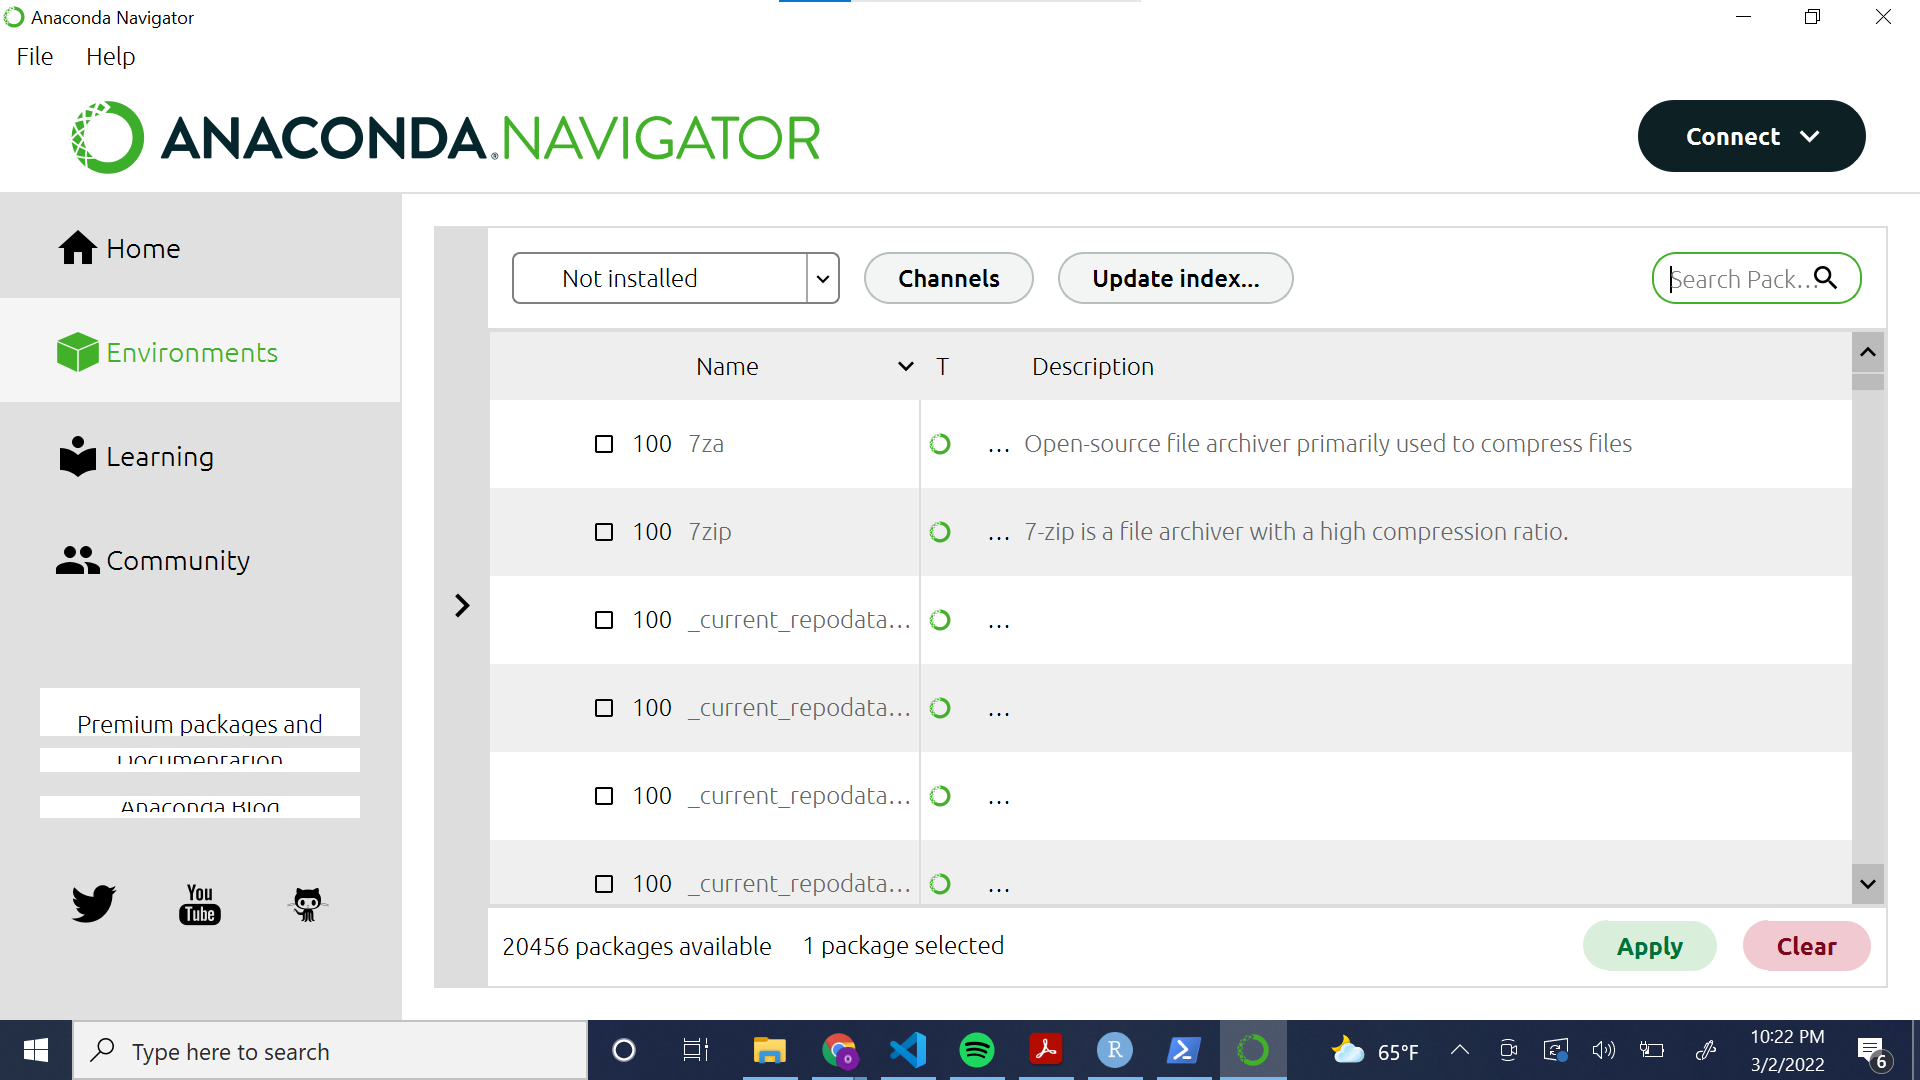
\includegraphics[width=26.67in]{images/anaconda_gui_install}

The following screenshot illustrates how to install a library to the ``base'' environment using the Anaconda Command Prompt.

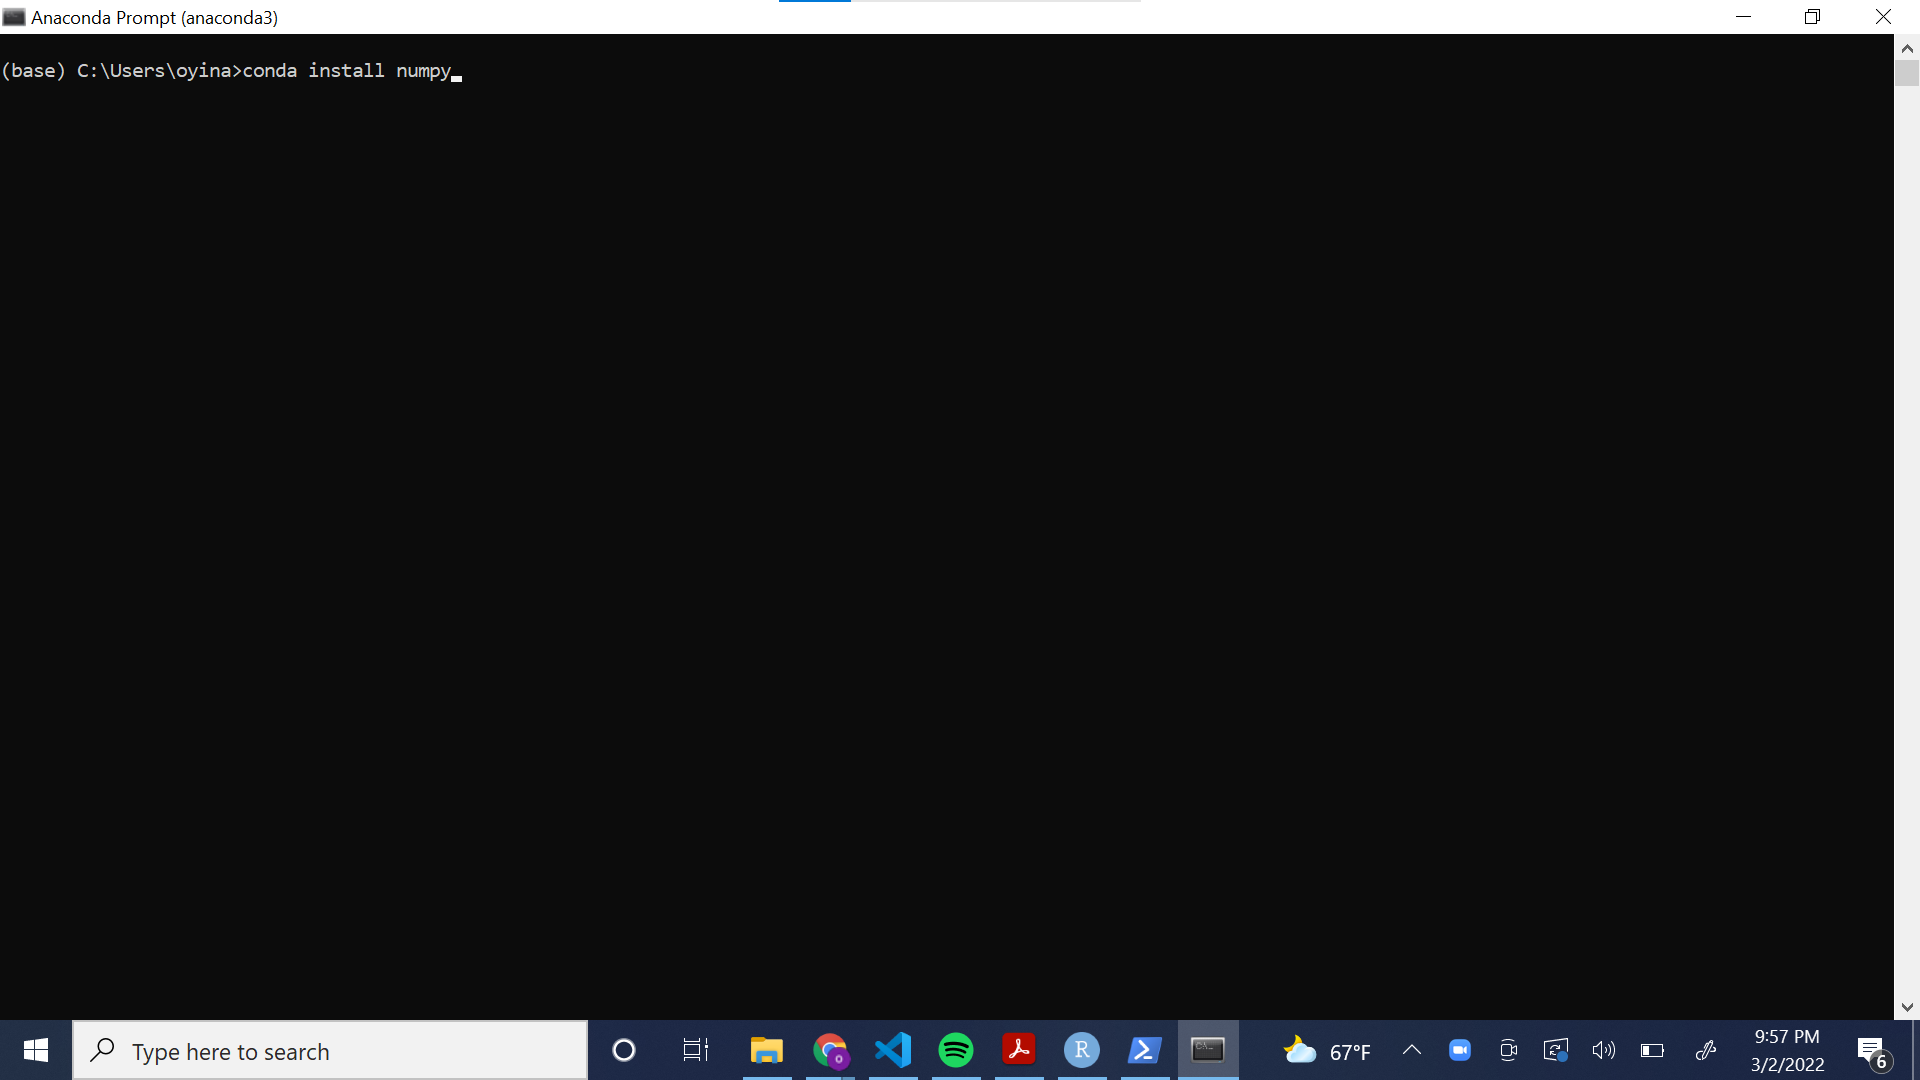
\includegraphics[width=26.67in]{images/anaconda_command_install}

Sometimes the commands to download libraries are not as simple as shown in the above example. The Anaconda website provides commands for how to download popular Python libraries.

\hypertarget{r-3}{%
\subsubsection*{R}\label{r-3}}
\addcontentsline{toc}{subsubsection}{R}

The main repository for R packages is the \href{https://cran.r-project.org/}{Comprehensive R Archive Network} (CRAN). Another repository is \href{https://www.bioconductor.org/}{Bioconductor}, which provides tools for working with genomic data. Many packages are also distributed on \href{https://github.com/}{GitHub}.

To install packages from CRAN use the \texttt{install.packages()} function. In RStudio, you can also go to Tools\ldots Install Packages\ldots{} for a dialog that will auto-complete package names as you type.

\begin{Shaded}
\begin{Highlighting}[]
\SpecialCharTok{\textgreater{}} \CommentTok{\# install the vcd package, a package for Visualizing Categorical Data}
\ErrorTok{\textgreater{}} \FunctionTok{install.packages}\NormalTok{(}\StringTok{"vcd"}\NormalTok{)}
\SpecialCharTok{\textgreater{}} 
\ErrorTok{\textgreater{}} \CommentTok{\# load the package}
\ErrorTok{\textgreater{}} \FunctionTok{library}\NormalTok{(vcd)}
\SpecialCharTok{\textgreater{}} 
\ErrorTok{\textgreater{}} \CommentTok{\# see which packages on your computer have updates available}
\ErrorTok{\textgreater{}} \FunctionTok{old.packages}\NormalTok{()}
\SpecialCharTok{\textgreater{}} 
\ErrorTok{\textgreater{}} \CommentTok{\# download and install available package updates;}
\ErrorTok{\textgreater{}} \CommentTok{\# set ask = TRUE to verify installation of each package}
\ErrorTok{\textgreater{}} \FunctionTok{update.packages}\NormalTok{(}\AttributeTok{ask =} \ConstantTok{FALSE}\NormalTok{)}
\end{Highlighting}
\end{Shaded}

To install R packages from GitHub use the \texttt{install\_github()} function from the \textbf{devtools} package. You need to include the username of the repo owner followed by a forward slash and the name of the package. Typing two colons between a package and a function in the package allows you to use that function without loading the package. That's how we use \texttt{install\_github()} below.

\begin{Shaded}
\begin{Highlighting}[]
\SpecialCharTok{\textgreater{}} \FunctionTok{install.packages}\NormalTok{(}\StringTok{"devtools"}\NormalTok{)}
\SpecialCharTok{\textgreater{}}\NormalTok{ devtools}\SpecialCharTok{::}\FunctionTok{install\_github}\NormalTok{(}\StringTok{"username/packagename"}\NormalTok{)}
\end{Highlighting}
\end{Shaded}

Occasionally when installing package updates you will be asked, ``Do you want to install from sources the package which needs compilation?'' R packages on CRAN are \emph{compiled} for Mac and Windows operating systems. That can take a day or two after a package has been submitted to CRAN. If you try to install a package that has not been compiled then you'll get asked the question above. If you click \emph{Yes}, R will try to compile the package on your computer. This will only work if you have the required build tools on your computer. For Windows this means having \href{https://cran.r-project.org/bin/windows/Rtools/}{Rtools} installed. Mac users should already have the necessary build tools. Unless you absolutely need the latest version of a package, it's probably fine to click \emph{No}.

\hypertarget{logic}{%
\section{Logic}\label{logic}}

Python and R share the same relational operators for making comparisons:

\begin{itemize}
\tightlist
\item
  \texttt{==} (equals)
\item
  \texttt{!=} (not equal to)
\item
  \texttt{\textless{}} (less than)
\item
  \texttt{\textless{}=} (less than or equal to)
\item
  \texttt{\textgreater{}} (greater than)
\item
  \texttt{\textgreater{}=} (greater than or equal to)
\end{itemize}

Likewise they share the same operators for logical AND and OR:

\begin{itemize}
\tightlist
\item
  \texttt{\&} (AND)
\item
  \texttt{\textbar{}} (OR)
\end{itemize}

However R also has \texttt{\&\&} and \texttt{\textbar{}\textbar{}} operators for programming control-flow.

Python and R have different operators for negation. Python uses \texttt{not}. R uses \texttt{!}.

\hypertarget{python-4}{%
\subsubsection*{Python}\label{python-4}}
\addcontentsline{toc}{subsubsection}{Python}

These Python operators can be used to compare arrays to single values or other arrays. This operation returns an array containing true and false values.

\begin{Shaded}
\begin{Highlighting}[]
\OperatorTok{\textgreater{}} \ImportTok{import}\NormalTok{ numpy }\ImportTok{as}\NormalTok{ np }
\OperatorTok{+} 
\OperatorTok{+} \CommentTok{\# Comparison of array to single value}
\OperatorTok{+}\NormalTok{ x1 }\OperatorTok{=}\NormalTok{ np.array([}\DecValTok{1}\NormalTok{,}\DecValTok{5}\NormalTok{,}\DecValTok{9}\NormalTok{,}\DecValTok{12}\NormalTok{,}\DecValTok{11}\NormalTok{,}\DecValTok{6}\NormalTok{])}
\OperatorTok{+}\NormalTok{ x1 }\OperatorTok{\textless{}} \DecValTok{8}
\OperatorTok{+} 
\OperatorTok{+} \CommentTok{\# Comparison of array to another array }
\NormalTok{array([ }\VariableTok{True}\NormalTok{,  }\VariableTok{True}\NormalTok{, }\VariableTok{False}\NormalTok{, }\VariableTok{False}\NormalTok{, }\VariableTok{False}\NormalTok{,  }\VariableTok{True}\NormalTok{])}
\OperatorTok{\textgreater{}}\NormalTok{ x2 }\OperatorTok{=}\NormalTok{ np.array([}\DecValTok{2}\NormalTok{,}\DecValTok{4}\NormalTok{,}\DecValTok{6}\NormalTok{,}\DecValTok{14}\NormalTok{,}\DecValTok{15}\NormalTok{,}\DecValTok{7}\NormalTok{])}
\OperatorTok{+}\NormalTok{ x1 }\OperatorTok{\textgreater{}}\NormalTok{ x2}
\NormalTok{array([}\VariableTok{False}\NormalTok{,  }\VariableTok{True}\NormalTok{,  }\VariableTok{True}\NormalTok{, }\VariableTok{False}\NormalTok{, }\VariableTok{False}\NormalTok{, }\VariableTok{False}\NormalTok{])}
\end{Highlighting}
\end{Shaded}

We can make multiple comparisons with the AND (\texttt{and}) and OR (\texttt{or}) operators. An important thing to note is that the \texttt{and} operator is inclusive, meaning that all statements must be true to return \texttt{True}. The \texttt{or} operator is exclusive, meaning that at least one of the statements joined by \texttt{or} must be true to return \texttt{True}.

\begin{Shaded}
\begin{Highlighting}[]
\OperatorTok{\textgreater{}}\NormalTok{ x}\OperatorTok{=}\DecValTok{5} 
\OperatorTok{+}\NormalTok{ y}\OperatorTok{=} \DecValTok{4}
\OperatorTok{+} 
\OperatorTok{+}\NormalTok{ x }\OperatorTok{\textgreater{}} \DecValTok{6} \KeywordTok{and}\NormalTok{ y }\OperatorTok{\textless{}} \DecValTok{10}
\VariableTok{False}
\OperatorTok{\textgreater{}}\NormalTok{ x }\OperatorTok{\textgreater{}} \DecValTok{6} \KeywordTok{or}\NormalTok{ y }\OperatorTok{\textless{}} \DecValTok{10}
\VariableTok{True}
\end{Highlighting}
\end{Shaded}

True and False operators have numeric values of 1 and 0, respectively. We can sum and average these values.

\begin{Shaded}
\begin{Highlighting}[]
\OperatorTok{\textgreater{}} \CommentTok{\# Sum of values greater than 10 in array x2}
\OperatorTok{+}\NormalTok{ np.}\BuiltInTok{sum}\NormalTok{(x2 }\OperatorTok{\textgreater{}} \DecValTok{10}\NormalTok{)}
\OperatorTok{+} 
\OperatorTok{+} \CommentTok{\# Portion of values greater than 10 in array x2}
\DecValTok{2}
\OperatorTok{\textgreater{}}\NormalTok{ np.mean(x2 }\OperatorTok{\textgreater{}} \DecValTok{10}\NormalTok{)}
\FloatTok{0.3333333333333333}
\end{Highlighting}
\end{Shaded}

\hypertarget{r-4}{%
\subsubsection*{R}\label{r-4}}
\addcontentsline{toc}{subsubsection}{R}

R's relational operators allow comparisons between a vector and a single value, or comparisons between two vectors. The result is a vector of TRUE/FALSE values.

\begin{Shaded}
\begin{Highlighting}[]
\SpecialCharTok{\textgreater{}} \CommentTok{\# vector compared with value}
\ErrorTok{\textgreater{}}\NormalTok{ x1 }\OtherTok{\textless{}{-}} \FunctionTok{c}\NormalTok{(}\DecValTok{1}\NormalTok{, }\DecValTok{5}\NormalTok{, }\DecValTok{9}\NormalTok{, }\DecValTok{12}\NormalTok{, }\DecValTok{11}\NormalTok{, }\DecValTok{6}\NormalTok{)}
\SpecialCharTok{\textgreater{}}\NormalTok{ x1 }\SpecialCharTok{\textless{}} \DecValTok{8}
\NormalTok{[}\DecValTok{1}\NormalTok{]  }\ConstantTok{TRUE}  \ConstantTok{TRUE} \ConstantTok{FALSE} \ConstantTok{FALSE} \ConstantTok{FALSE}  \ConstantTok{TRUE}
\SpecialCharTok{\textgreater{}} 
\ErrorTok{\textgreater{}} \CommentTok{\# vector compared with vector}
\ErrorTok{\textgreater{}}\NormalTok{ x2 }\OtherTok{\textless{}{-}} \FunctionTok{c}\NormalTok{(}\DecValTok{2}\NormalTok{, }\DecValTok{4}\NormalTok{, }\DecValTok{6}\NormalTok{, }\DecValTok{14}\NormalTok{, }\DecValTok{15}\NormalTok{, }\DecValTok{7}\NormalTok{)}
\SpecialCharTok{\textgreater{}}\NormalTok{ x1 }\SpecialCharTok{\textgreater{}}\NormalTok{ x2}
\NormalTok{[}\DecValTok{1}\NormalTok{] }\ConstantTok{FALSE}  \ConstantTok{TRUE}  \ConstantTok{TRUE} \ConstantTok{FALSE} \ConstantTok{FALSE} \ConstantTok{FALSE}
\end{Highlighting}
\end{Shaded}

Comparisons with NA (missing value) results in NA.

\begin{Shaded}
\begin{Highlighting}[]
\SpecialCharTok{\textgreater{}}\NormalTok{ x1 }\OtherTok{\textless{}{-}} \FunctionTok{c}\NormalTok{(}\DecValTok{1}\NormalTok{, }\DecValTok{5}\NormalTok{, }\DecValTok{9}\NormalTok{, }\ConstantTok{NA}\NormalTok{, }\DecValTok{11}\NormalTok{, }\DecValTok{6}\NormalTok{)}
\SpecialCharTok{\textgreater{}}\NormalTok{ x1 }\SpecialCharTok{\textless{}} \DecValTok{8}
\NormalTok{[}\DecValTok{1}\NormalTok{]  }\ConstantTok{TRUE}  \ConstantTok{TRUE} \ConstantTok{FALSE}    \ConstantTok{NA} \ConstantTok{FALSE}  \ConstantTok{TRUE}
\end{Highlighting}
\end{Shaded}

Multiple comparisons can be made with AND (\texttt{\&}) and OR (\texttt{\textbar{}}) operators.

\begin{Shaded}
\begin{Highlighting}[]
\SpecialCharTok{\textgreater{}}\NormalTok{ x2 }\SpecialCharTok{\textgreater{}} \DecValTok{3} \SpecialCharTok{\&}\NormalTok{ x2 }\SpecialCharTok{\textless{}} \DecValTok{10}
\NormalTok{[}\DecValTok{1}\NormalTok{] }\ConstantTok{FALSE}  \ConstantTok{TRUE}  \ConstantTok{TRUE} \ConstantTok{FALSE} \ConstantTok{FALSE}  \ConstantTok{TRUE}
\SpecialCharTok{\textgreater{}}\NormalTok{ x2 }\SpecialCharTok{\textless{}} \DecValTok{3} \SpecialCharTok{|}\NormalTok{ x2 }\SpecialCharTok{\textgreater{}} \DecValTok{10}
\NormalTok{[}\DecValTok{1}\NormalTok{]  }\ConstantTok{TRUE} \ConstantTok{FALSE} \ConstantTok{FALSE}  \ConstantTok{TRUE}  \ConstantTok{TRUE} \ConstantTok{FALSE}
\end{Highlighting}
\end{Shaded}

TRUE/FALSE values in R have numeric values of 1/0. This allows us to sum and average them. (Note: an average of 0 and 1 values is the proportion of 1's.)

\begin{Shaded}
\begin{Highlighting}[]
\SpecialCharTok{\textgreater{}} \CommentTok{\# sum of values greater than 10}
\ErrorTok{\textgreater{}} \FunctionTok{sum}\NormalTok{(x2 }\SpecialCharTok{\textgreater{}} \DecValTok{10}\NormalTok{)}
\NormalTok{[}\DecValTok{1}\NormalTok{] }\DecValTok{2}
\SpecialCharTok{\textgreater{}} 
\ErrorTok{\textgreater{}} \CommentTok{\# proportion of values greater than 10}
\ErrorTok{\textgreater{}} \FunctionTok{mean}\NormalTok{(x2 }\SpecialCharTok{\textgreater{}} \DecValTok{10}\NormalTok{)}
\NormalTok{[}\DecValTok{1}\NormalTok{] }\FloatTok{0.3333333}
\end{Highlighting}
\end{Shaded}

Use the \texttt{!} operator for negation. This allows to check for something that is NOT TRUE.

\begin{Shaded}
\begin{Highlighting}[]
\SpecialCharTok{\textgreater{}} \CommentTok{\# which value are NOT less than 6}
\ErrorTok{\textgreater{}} \SpecialCharTok{!}\NormalTok{x2 }\SpecialCharTok{\textless{}} \DecValTok{6}
\NormalTok{[}\DecValTok{1}\NormalTok{] }\ConstantTok{FALSE} \ConstantTok{FALSE}  \ConstantTok{TRUE}  \ConstantTok{TRUE}  \ConstantTok{TRUE}  \ConstantTok{TRUE}
\end{Highlighting}
\end{Shaded}

See the \texttt{?Comparison} and \texttt{?Logic} help pages for more information.

\hypertarget{generating-a-sequence-of-values}{%
\section{Generating a sequence of values}\label{generating-a-sequence-of-values}}

In Python, one option for generating a sequence of values is \texttt{arange()} from \textbf{NumPy}. In R, a common approach is to use \texttt{seq()}. The sequences can be incremented by indicating a \texttt{step} argument in \texttt{arange()} or a \texttt{by} argument in \texttt{seq()}. Be aware that the end of the start/stop interval in \texttt{arange()} is \emph{open}, but both sides of the from/to interval in \texttt{seq()} are \emph{closed}.

\hypertarget{python-5}{%
\subsubsection*{Python}\label{python-5}}
\addcontentsline{toc}{subsubsection}{Python}

\begin{Shaded}
\begin{Highlighting}[]
\OperatorTok{\textgreater{}} \ImportTok{import}\NormalTok{ numpy }\ImportTok{as}\NormalTok{ np}
\OperatorTok{+}\NormalTok{ x }\OperatorTok{=}\NormalTok{ np.arange(start }\OperatorTok{=} \DecValTok{1}\NormalTok{, stop }\OperatorTok{=} \DecValTok{11}\NormalTok{, step }\OperatorTok{=} \DecValTok{2}\NormalTok{)}
\OperatorTok{+}\NormalTok{ x}
\NormalTok{array([}\DecValTok{1}\NormalTok{, }\DecValTok{3}\NormalTok{, }\DecValTok{5}\NormalTok{, }\DecValTok{7}\NormalTok{, }\DecValTok{9}\NormalTok{])}
\end{Highlighting}
\end{Shaded}

\hypertarget{r-5}{%
\subsubsection*{R}\label{r-5}}
\addcontentsline{toc}{subsubsection}{R}

\begin{Shaded}
\begin{Highlighting}[]
\SpecialCharTok{\textgreater{}}\NormalTok{ x }\OtherTok{\textless{}{-}} \FunctionTok{seq}\NormalTok{(}\AttributeTok{from =} \DecValTok{1}\NormalTok{, }\AttributeTok{to =} \DecValTok{11}\NormalTok{, }\AttributeTok{by =} \DecValTok{2}\NormalTok{)}
\SpecialCharTok{\textgreater{}}\NormalTok{ x}
\NormalTok{[}\DecValTok{1}\NormalTok{]  }\DecValTok{1}  \DecValTok{3}  \DecValTok{5}  \DecValTok{7}  \DecValTok{9} \DecValTok{11}
\end{Highlighting}
\end{Shaded}

\hypertarget{calculating-means-and-medians}{%
\section{Calculating means and medians}\label{calculating-means-and-medians}}

The \textbf{NumPy} Python library has functions for calculating means and medians, and base R has functions for doing the same.

\hypertarget{python-6}{%
\subsubsection*{Python}\label{python-6}}
\addcontentsline{toc}{subsubsection}{Python}

Mean, using function from \textbf{NumPy} library

\begin{Shaded}
\begin{Highlighting}[]
\OperatorTok{\textgreater{}} \ImportTok{import}\NormalTok{ numpy }\ImportTok{as}\NormalTok{ np}
\OperatorTok{+}\NormalTok{ x }\OperatorTok{=}\NormalTok{ [}\DecValTok{90}\NormalTok{, }\DecValTok{105}\NormalTok{, }\DecValTok{110}\NormalTok{]}
\OperatorTok{+}\NormalTok{ x\_avg }\OperatorTok{=}\NormalTok{ np.mean(x)}
\OperatorTok{+} \BuiltInTok{print}\NormalTok{(x\_avg)}
\FloatTok{101.66666666666667}
\end{Highlighting}
\end{Shaded}

Median, using function from \textbf{NumPy} library

\begin{Shaded}
\begin{Highlighting}[]
\OperatorTok{\textgreater{}}\NormalTok{ x }\OperatorTok{=}\NormalTok{ [}\DecValTok{98}\NormalTok{, }\DecValTok{102}\NormalTok{, }\DecValTok{20}\NormalTok{, }\DecValTok{22}\NormalTok{, }\DecValTok{304}\NormalTok{]}
\OperatorTok{+}\NormalTok{ x\_med }\OperatorTok{=}\NormalTok{ np.median(x)}
\OperatorTok{+} \BuiltInTok{print}\NormalTok{(x\_med)}
\FloatTok{98.0}
\end{Highlighting}
\end{Shaded}

\hypertarget{r-6}{%
\subsubsection*{R}\label{r-6}}
\addcontentsline{toc}{subsubsection}{R}

Mean, using function from base R

\begin{Shaded}
\begin{Highlighting}[]
\SpecialCharTok{\textgreater{}}\NormalTok{ x }\OtherTok{\textless{}{-}} \FunctionTok{c}\NormalTok{(}\DecValTok{90}\NormalTok{, }\DecValTok{105}\NormalTok{, }\DecValTok{110}\NormalTok{)}
\SpecialCharTok{\textgreater{}}\NormalTok{ x\_avg }\OtherTok{\textless{}{-}} \FunctionTok{mean}\NormalTok{(x)}
\SpecialCharTok{\textgreater{}}\NormalTok{ x\_avg}
\NormalTok{[}\DecValTok{1}\NormalTok{] }\FloatTok{101.6667}
\end{Highlighting}
\end{Shaded}

Median, using function from base R

\begin{Shaded}
\begin{Highlighting}[]
\SpecialCharTok{\textgreater{}}\NormalTok{ x }\OtherTok{\textless{}{-}} \FunctionTok{c}\NormalTok{(}\DecValTok{98}\NormalTok{, }\DecValTok{102}\NormalTok{, }\DecValTok{20}\NormalTok{, }\DecValTok{22}\NormalTok{, }\DecValTok{304}\NormalTok{)}
\SpecialCharTok{\textgreater{}}\NormalTok{ x\_med }\OtherTok{\textless{}{-}} \FunctionTok{median}\NormalTok{(x)}
\SpecialCharTok{\textgreater{}}\NormalTok{ x\_med}
\NormalTok{[}\DecValTok{1}\NormalTok{] }\DecValTok{98}
\end{Highlighting}
\end{Shaded}

\hypertarget{writing-your-own-functions}{%
\section{Writing your own functions}\label{writing-your-own-functions}}

Python and R allow and encourage users to create their own functions. Functions can be created, named, and stored in memory and used throughout a session. Or they can be created on-the-fly ``anonymously'' and used once.

\hypertarget{python-7}{%
\subsubsection*{Python}\label{python-7}}
\addcontentsline{toc}{subsubsection}{Python}

Functions in Python are defined by using the \texttt{def} keyword followed by the name we choose for our function with its arguments inside parentheses. We must include a \texttt{return()} statement after the body of our function to indicate the end of the function. The return statement takes an optional argument in its parentheses that will be the output of the function. Here we create a function to calculate the standard error of a mean (SEM) and call it \texttt{SEM}.

\begin{Shaded}
\begin{Highlighting}[]
\OperatorTok{\textgreater{}} \KeywordTok{def}\NormalTok{ SEM(x):}
\OperatorTok{+}   \ImportTok{import}\NormalTok{ numpy }\ImportTok{as}\NormalTok{ np }\CommentTok{\# import statement included inside the function to ensure it\textquotesingle{}s always imported}
\OperatorTok{+}\NormalTok{   s }\OperatorTok{=}\NormalTok{ x.std(ddof}\OperatorTok{=}\DecValTok{1}\NormalTok{) }\CommentTok{\# find standard deviation of the data, specify delta degrees of freedom as 1 (makes denominator n{-}1 not n)}
\OperatorTok{+}\NormalTok{   n }\OperatorTok{=}\NormalTok{ x.shape[}\DecValTok{0}\NormalTok{] }\CommentTok{\# extract the length of the input array}
\OperatorTok{+}\NormalTok{   sem }\OperatorTok{=}\NormalTok{ s }\OperatorTok{/}\NormalTok{ np.sqrt(n) }\CommentTok{\# calculate the SEM}
\OperatorTok{+}   \ControlFlowTok{return}\NormalTok{(sem) }\CommentTok{\# return the calculated SEM value}
\end{Highlighting}
\end{Shaded}

Now let's try our function out on some test data.

\begin{Shaded}
\begin{Highlighting}[]
\OperatorTok{\textgreater{}}\NormalTok{ d }\OperatorTok{=}\NormalTok{ np.array([}\DecValTok{3}\NormalTok{,}\DecValTok{4}\NormalTok{,}\DecValTok{4}\NormalTok{,}\DecValTok{7}\NormalTok{,}\DecValTok{9}\NormalTok{,}\DecValTok{6}\NormalTok{,}\DecValTok{2}\NormalTok{,}\DecValTok{5}\NormalTok{,}\DecValTok{7}\NormalTok{])}
\OperatorTok{+}\NormalTok{ SEM(d)}
\FloatTok{0.7412035591181296}
\end{Highlighting}
\end{Shaded}

Oftentimes functions have built-in error-checking that returns messages describing the error. Here we show a simple error-check to ensure that the argument passed to our function is a number.

\begin{Shaded}
\begin{Highlighting}[]
\OperatorTok{\textgreater{}} \KeywordTok{def}\NormalTok{ SEM(x):}
\OperatorTok{+}   \ImportTok{import}\NormalTok{ numpy }\ImportTok{as}\NormalTok{ np}
\OperatorTok{+}   
\OperatorTok{+}   \ControlFlowTok{if}\NormalTok{ np.issubdtype(x.dtype,np.number)}\OperatorTok{==}\VariableTok{False}\NormalTok{:}
\OperatorTok{+}     \ControlFlowTok{raise} \PreprocessorTok{ValueError}\NormalTok{(}\StringTok{"Data must be numeric"}\NormalTok{)}
\OperatorTok{+}   
\OperatorTok{+}\NormalTok{   s }\OperatorTok{=}\NormalTok{ x.std(ddof}\OperatorTok{=}\DecValTok{1}\NormalTok{) }
\OperatorTok{+}\NormalTok{   n }\OperatorTok{=}\NormalTok{ x.shape[}\DecValTok{0}\NormalTok{] }
\OperatorTok{+}\NormalTok{   sem }\OperatorTok{=}\NormalTok{ s }\OperatorTok{/}\NormalTok{ np.sqrt(n) }
\OperatorTok{+}   \ControlFlowTok{return}\NormalTok{(sem) }
\end{Highlighting}
\end{Shaded}

Python functions can return more than one result. It will output the results into a \texttt{tuple}. A tuple is a data structure very similar to a list, but it is immutable - we cannot change the order of the entries. Here we make our function return both the mean and the SEM of our data.

\begin{Shaded}
\begin{Highlighting}[]
\OperatorTok{\textgreater{}} \KeywordTok{def}\NormalTok{ SEM(x):}
\OperatorTok{+}   \ImportTok{import}\NormalTok{ numpy }\ImportTok{as}\NormalTok{ np}
\OperatorTok{+}   
\OperatorTok{+}   \ControlFlowTok{if}\NormalTok{ np.issubdtype(x.dtype,np.number)}\OperatorTok{==}\VariableTok{False}\NormalTok{:}
\OperatorTok{+}     \ControlFlowTok{raise} \PreprocessorTok{ValueError}\NormalTok{(}\StringTok{"Data must be numeric"}\NormalTok{)}
\OperatorTok{+}   
\OperatorTok{+}\NormalTok{   s }\OperatorTok{=}\NormalTok{ x.std(ddof}\OperatorTok{=}\DecValTok{1}\NormalTok{) }
\OperatorTok{+}\NormalTok{   n }\OperatorTok{=}\NormalTok{ x.shape[}\DecValTok{0}\NormalTok{] }
\OperatorTok{+}\NormalTok{   sem }\OperatorTok{=}\NormalTok{ s }\OperatorTok{/}\NormalTok{ np.sqrt(n) }
\OperatorTok{+}   
\OperatorTok{+}\NormalTok{   m }\OperatorTok{=}\NormalTok{ np.mean(x)}
\OperatorTok{+}   \ControlFlowTok{return}\NormalTok{(sem,m) }
\end{Highlighting}
\end{Shaded}

\hypertarget{r-7}{%
\subsubsection*{R}\label{r-7}}
\addcontentsline{toc}{subsubsection}{R}

Functions in R can be created and named using \texttt{function()}. Add arguments inside the parentheses. Longer functions with multiple lines can be wrapped in curly braces \texttt{\{\}}.

Below we create a function to calculate the standard error of a mean (SEM) and name it \texttt{sem}. It takes one argument: \texttt{x}, a vector of numbers. Both the function name and argument name(s) can be whatever we like, as long as they follow \href{https://cran.r-project.org/doc/manuals/r-release/R-intro.html\#R-commands_003b-case-sensitivity-etc}{R's naming conventions}.

\begin{Shaded}
\begin{Highlighting}[]
\SpecialCharTok{\textgreater{}}\NormalTok{ sem }\OtherTok{\textless{}{-}} \ControlFlowTok{function}\NormalTok{(x)\{}
\SpecialCharTok{+}\NormalTok{   s }\OtherTok{\textless{}{-}} \FunctionTok{sd}\NormalTok{(x)}
\SpecialCharTok{+}\NormalTok{   n }\OtherTok{\textless{}{-}} \FunctionTok{length}\NormalTok{(x)}
\SpecialCharTok{+}\NormalTok{   s}\SpecialCharTok{/}\FunctionTok{sqrt}\NormalTok{(n)}
\SpecialCharTok{+}\NormalTok{ \}}
\end{Highlighting}
\end{Shaded}

Now we can try it out on some test data.

\begin{Shaded}
\begin{Highlighting}[]
\SpecialCharTok{\textgreater{}}\NormalTok{ d }\OtherTok{\textless{}{-}} \FunctionTok{c}\NormalTok{(}\DecValTok{3}\NormalTok{,}\DecValTok{4}\NormalTok{,}\DecValTok{4}\NormalTok{,}\DecValTok{7}\NormalTok{,}\DecValTok{9}\NormalTok{,}\DecValTok{6}\NormalTok{,}\DecValTok{2}\NormalTok{,}\DecValTok{5}\NormalTok{,}\DecValTok{7}\NormalTok{)}
\SpecialCharTok{\textgreater{}} \FunctionTok{sem}\NormalTok{(d)}
\NormalTok{[}\DecValTok{1}\NormalTok{] }\FloatTok{0.7412036}
\end{Highlighting}
\end{Shaded}

Functions that will be used on different data and/or by different users often need built-in error-checking to return informative error messages. This simple example checks if the data are not numeric and returns a special error message.

\begin{Shaded}
\begin{Highlighting}[]
\SpecialCharTok{\textgreater{}}\NormalTok{ sem }\OtherTok{\textless{}{-}} \ControlFlowTok{function}\NormalTok{(x)\{}
\SpecialCharTok{+}   \ControlFlowTok{if}\NormalTok{(}\SpecialCharTok{!}\FunctionTok{is.numeric}\NormalTok{(x)) }\FunctionTok{stop}\NormalTok{(}\StringTok{"x must be numeric"}\NormalTok{)}
\SpecialCharTok{+}\NormalTok{   s }\OtherTok{\textless{}{-}} \FunctionTok{sd}\NormalTok{(x)}
\SpecialCharTok{+}\NormalTok{   n }\OtherTok{\textless{}{-}} \FunctionTok{length}\NormalTok{(x)}
\SpecialCharTok{+}\NormalTok{   s}\SpecialCharTok{/}\FunctionTok{sqrt}\NormalTok{(n)}
\SpecialCharTok{+}\NormalTok{ \}}
\SpecialCharTok{\textgreater{}} \FunctionTok{sem}\NormalTok{(}\FunctionTok{c}\NormalTok{(}\DecValTok{1}\NormalTok{, }\DecValTok{4}\NormalTok{, }\DecValTok{6}\NormalTok{, }\StringTok{"a"}\NormalTok{))}
\NormalTok{Error }\ControlFlowTok{in} \FunctionTok{sem}\NormalTok{(}\FunctionTok{c}\NormalTok{(}\DecValTok{1}\NormalTok{, }\DecValTok{4}\NormalTok{, }\DecValTok{6}\NormalTok{, }\StringTok{"a"}\NormalTok{))}\SpecialCharTok{:}\NormalTok{ x must be numeric}
\end{Highlighting}
\end{Shaded}

R functions can also return more than one result. Below we return a list that holds the mean and SEM, but we could also return a vector, a data frame, or other data structure. Notice we also add an additional argument, \texttt{...}, known as the three dots argument. This allows us to pass arguments for \texttt{sd} and \texttt{mean} directly through our own function. Below we pass through \texttt{na.rm\ =\ TRUE} to drop missing values.

\begin{Shaded}
\begin{Highlighting}[]
\SpecialCharTok{\textgreater{}}\NormalTok{ sem }\OtherTok{\textless{}{-}} \ControlFlowTok{function}\NormalTok{(x, ...)\{}
\SpecialCharTok{+}   \ControlFlowTok{if}\NormalTok{(}\SpecialCharTok{!}\FunctionTok{is.numeric}\NormalTok{(x)) }\FunctionTok{stop}\NormalTok{(}\StringTok{"x must be numeric"}\NormalTok{)}
\SpecialCharTok{+}\NormalTok{   s }\OtherTok{\textless{}{-}} \FunctionTok{sd}\NormalTok{(x, ...)}
\SpecialCharTok{+}\NormalTok{   n }\OtherTok{\textless{}{-}} \FunctionTok{length}\NormalTok{(x)}
\SpecialCharTok{+}\NormalTok{   se }\OtherTok{\textless{}{-}}\NormalTok{ s}\SpecialCharTok{/}\FunctionTok{sqrt}\NormalTok{(n)}
\SpecialCharTok{+}\NormalTok{   mean }\OtherTok{\textless{}{-}} \FunctionTok{mean}\NormalTok{(x, ...)}
\SpecialCharTok{+}   \FunctionTok{list}\NormalTok{(}\AttributeTok{mean =}\NormalTok{ mean, }\AttributeTok{SEM =}\NormalTok{ se)}
\SpecialCharTok{+}\NormalTok{ \}}
\SpecialCharTok{\textgreater{}} 
\ErrorTok{\textgreater{}}\NormalTok{ d }\OtherTok{\textless{}{-}} \FunctionTok{c}\NormalTok{(}\DecValTok{1}\NormalTok{, }\DecValTok{4}\NormalTok{, }\DecValTok{6}\NormalTok{, }\DecValTok{8}\NormalTok{, }\ConstantTok{NA}\NormalTok{, }\DecValTok{4}\NormalTok{, }\DecValTok{4}\NormalTok{, }\DecValTok{8}\NormalTok{, }\DecValTok{6}\NormalTok{)}
\SpecialCharTok{\textgreater{}} \FunctionTok{sem}\NormalTok{(d, }\AttributeTok{na.rm =} \ConstantTok{TRUE}\NormalTok{)}
\SpecialCharTok{$}\NormalTok{mean}
\NormalTok{[}\DecValTok{1}\NormalTok{] }\FloatTok{5.125}

\SpecialCharTok{$}\NormalTok{SEM}
\NormalTok{[}\DecValTok{1}\NormalTok{] }\FloatTok{0.7855339}
\end{Highlighting}
\end{Shaded}

Functions can also be created on-the-fly as ``anonymous'' functions. This simply means the functions are not saved as objects in memory. These are often used with R's family of \texttt{apply} functions. As before, the functions can be created with \texttt{function()}. We can also use the backslash \texttt{\textbackslash{}} as a shorthand for \texttt{function()}. We demonstrate both below with a data frame.

\begin{Shaded}
\begin{Highlighting}[]
\SpecialCharTok{\textgreater{}} \CommentTok{\# generate some example data}
\ErrorTok{\textgreater{}}\NormalTok{ d }\OtherTok{\textless{}{-}} \FunctionTok{data.frame}\NormalTok{(}\AttributeTok{x1 =} \FunctionTok{c}\NormalTok{(}\DecValTok{3}\NormalTok{, }\DecValTok{5}\NormalTok{, }\DecValTok{7}\NormalTok{, }\DecValTok{1}\NormalTok{, }\DecValTok{5}\NormalTok{, }\DecValTok{4}\NormalTok{),}
\SpecialCharTok{+}                 \AttributeTok{x2 =} \FunctionTok{c}\NormalTok{(}\DecValTok{6}\NormalTok{, }\DecValTok{9}\NormalTok{, }\DecValTok{8}\NormalTok{, }\DecValTok{9}\NormalTok{, }\DecValTok{2}\NormalTok{, }\DecValTok{5}\NormalTok{),}
\SpecialCharTok{+}                 \AttributeTok{x3 =} \FunctionTok{c}\NormalTok{(}\DecValTok{1}\NormalTok{, }\DecValTok{9}\NormalTok{, }\DecValTok{9}\NormalTok{, }\DecValTok{7}\NormalTok{, }\DecValTok{8}\NormalTok{, }\DecValTok{4}\NormalTok{))}
\SpecialCharTok{\textgreater{}}\NormalTok{ d}
\NormalTok{  x1 x2 x3}
\DecValTok{1}  \DecValTok{3}  \DecValTok{6}  \DecValTok{1}
\DecValTok{2}  \DecValTok{5}  \DecValTok{9}  \DecValTok{9}
\DecValTok{3}  \DecValTok{7}  \DecValTok{8}  \DecValTok{9}
\DecValTok{4}  \DecValTok{1}  \DecValTok{9}  \DecValTok{7}
\DecValTok{5}  \DecValTok{5}  \DecValTok{2}  \DecValTok{8}
\DecValTok{6}  \DecValTok{4}  \DecValTok{5}  \DecValTok{4}
\end{Highlighting}
\end{Shaded}

Now find the standard error of the mean for the three columns using an anonymous function with \texttt{lapply()}. The ``l'' means the result will be a list. We apply the function to each column of the data frame.

\begin{Shaded}
\begin{Highlighting}[]
\SpecialCharTok{\textgreater{}} \FunctionTok{lapply}\NormalTok{(d, }\ControlFlowTok{function}\NormalTok{(x)}\FunctionTok{sd}\NormalTok{(x)}\SpecialCharTok{/}\FunctionTok{sqrt}\NormalTok{(}\FunctionTok{length}\NormalTok{(x)))}
\SpecialCharTok{$}\NormalTok{x1}
\NormalTok{[}\DecValTok{1}\NormalTok{] }\FloatTok{0.8333333}

\SpecialCharTok{$}\NormalTok{x2}
\NormalTok{[}\DecValTok{1}\NormalTok{] }\FloatTok{1.118034}

\SpecialCharTok{$}\NormalTok{x3}
\NormalTok{[}\DecValTok{1}\NormalTok{] }\FloatTok{1.308094}
\end{Highlighting}
\end{Shaded}

We can also use the backslash as a shorthand for \texttt{function()}.

\begin{Shaded}
\begin{Highlighting}[]
\SpecialCharTok{\textgreater{}} \FunctionTok{lapply}\NormalTok{(d, \textbackslash{}(x)}\FunctionTok{sd}\NormalTok{(x)}\SpecialCharTok{/}\FunctionTok{sqrt}\NormalTok{(}\FunctionTok{length}\NormalTok{(x)))}
\SpecialCharTok{$}\NormalTok{x1}
\NormalTok{[}\DecValTok{1}\NormalTok{] }\FloatTok{0.8333333}

\SpecialCharTok{$}\NormalTok{x2}
\NormalTok{[}\DecValTok{1}\NormalTok{] }\FloatTok{1.118034}

\SpecialCharTok{$}\NormalTok{x3}
\NormalTok{[}\DecValTok{1}\NormalTok{] }\FloatTok{1.308094}
\end{Highlighting}
\end{Shaded}

\hypertarget{data-structures}{%
\chapter{Data Structures}\label{data-structures}}

This chapter compares and contrasts data structures in Python and R.

\hypertarget{one-dimensional-data}{%
\section{One-dimensional data}\label{one-dimensional-data}}

A one-dimensional data structure can be visualized as a column in a spreadsheet or as a list of values.

\hypertarget{python-8}{%
\subsubsection*{Python}\label{python-8}}
\addcontentsline{toc}{subsubsection}{Python}

There are many ways to organize one-dimensional data in Python. Three of the most common one-dimensional data structures are lists, numpy arrays, and pandas Series. All three are ordered and mutable, and can contain data of different types.

Lists in Python do not need to be explicitly declared; they are indicated by the use of square brackets.

\begin{Shaded}
\begin{Highlighting}[]
\OperatorTok{\textgreater{}}\NormalTok{ l }\OperatorTok{=}\NormalTok{ [}\DecValTok{1}\NormalTok{,}\DecValTok{2}\NormalTok{,}\DecValTok{3}\NormalTok{,}\StringTok{\textquotesingle{}hello\textquotesingle{}}\NormalTok{]}
\end{Highlighting}
\end{Shaded}

Values in lists can be accessed by using square brackets. Python indexing begins at 0, so to extract the first element, we would use the index 0. Python also allows for negative indexing; using an index of -1 will return the last value in the list. Indexing a range in Python is not inclusive of the last index.

\begin{Shaded}
\begin{Highlighting}[]
\OperatorTok{\textgreater{}} \CommentTok{\# extract first element}
\OperatorTok{+}\NormalTok{ l[}\DecValTok{0}\NormalTok{]}
\OperatorTok{+} 
\OperatorTok{+} \CommentTok{\#extract last element}
\DecValTok{1}
\OperatorTok{\textgreater{}}\NormalTok{ l[}\OperatorTok{{-}}\DecValTok{1}\NormalTok{]}
\OperatorTok{+} 
\OperatorTok{+} \CommentTok{\# extract 2nd and 3rd elements}
\CommentTok{\textquotesingle{}hello\textquotesingle{}}
\OperatorTok{\textgreater{}}\NormalTok{ l[}\DecValTok{1}\NormalTok{:}\DecValTok{3}\NormalTok{]}
\NormalTok{[}\DecValTok{2}\NormalTok{, }\DecValTok{3}\NormalTok{]}
\end{Highlighting}
\end{Shaded}

Numpy arrays, on the other hand, need to be declared using the \texttt{numpy.array()} function, and the \textbf{numpy} package needs to be imported.

\begin{Shaded}
\begin{Highlighting}[]
\OperatorTok{\textgreater{}} \ImportTok{import}\NormalTok{ numpy }\ImportTok{as}\NormalTok{ np}
\OperatorTok{+} 
\OperatorTok{+}\NormalTok{ arr }\OperatorTok{=}\NormalTok{ np.array([}\DecValTok{1}\NormalTok{,}\DecValTok{2}\NormalTok{,}\DecValTok{3}\NormalTok{,}\StringTok{\textquotesingle{}hello\textquotesingle{}}\NormalTok{])}
\OperatorTok{+} \BuiltInTok{print}\NormalTok{(arr)}
\NormalTok{[}\StringTok{\textquotesingle{}1\textquotesingle{}} \StringTok{\textquotesingle{}2\textquotesingle{}} \StringTok{\textquotesingle{}3\textquotesingle{}} \StringTok{\textquotesingle{}hello\textquotesingle{}}\NormalTok{]}
\end{Highlighting}
\end{Shaded}

Accessing data in a numpy array is the same as indexing a list.

\begin{Shaded}
\begin{Highlighting}[]
\OperatorTok{\textgreater{}} \CommentTok{\# extract first element }
\OperatorTok{+}\NormalTok{ arr[}\DecValTok{0}\NormalTok{]}
\OperatorTok{+} 
\OperatorTok{+} \CommentTok{\# extract last element}
\CommentTok{\textquotesingle{}1\textquotesingle{}}
\OperatorTok{\textgreater{}}\NormalTok{ arr[}\OperatorTok{{-}}\DecValTok{1}\NormalTok{]}
\OperatorTok{+} 
\OperatorTok{+} \CommentTok{\# extract 2nd and 3rd elements}
\CommentTok{\textquotesingle{}hello\textquotesingle{}}
\OperatorTok{\textgreater{}}\NormalTok{ arr[}\DecValTok{1}\NormalTok{:}\DecValTok{3}\NormalTok{]}
\NormalTok{array([}\StringTok{\textquotesingle{}2\textquotesingle{}}\NormalTok{, }\StringTok{\textquotesingle{}3\textquotesingle{}}\NormalTok{], dtype}\OperatorTok{=}\StringTok{\textquotesingle{}\textless{}U11\textquotesingle{}}\NormalTok{)}
\end{Highlighting}
\end{Shaded}

Pandas Series also need to be declared using the \texttt{pandas.Series()} function. Like \textbf{numpy}, the \textbf{pandas} package must be imported as well. The pandas package is built on numpy, so we can input data into a pandas Series using a numpy array. We can extract data from the Series by using the index similar to indexing a list and numpy array.

\begin{Shaded}
\begin{Highlighting}[]
\OperatorTok{\textgreater{}} \ImportTok{import}\NormalTok{ pandas }\ImportTok{as}\NormalTok{ pd }
\OperatorTok{+} \ImportTok{import}\NormalTok{ numpy }\ImportTok{as}\NormalTok{ np}
\OperatorTok{+} 
\OperatorTok{+}\NormalTok{ data }\OperatorTok{=}\NormalTok{ np.array([}\DecValTok{1}\NormalTok{,}\DecValTok{2}\NormalTok{,}\DecValTok{3}\NormalTok{,}\StringTok{"hello"}\NormalTok{])}
\OperatorTok{+}\NormalTok{ ser1 }\OperatorTok{=}\NormalTok{ pd.Series(data)}
\OperatorTok{+} \BuiltInTok{print}\NormalTok{(ser1)}
\OperatorTok{+} 
\OperatorTok{+} \CommentTok{\# extract first element }
\DecValTok{0}        \DecValTok{1}
\DecValTok{1}        \DecValTok{2}
\DecValTok{2}        \DecValTok{3}
\DecValTok{3}\NormalTok{    hello}
\NormalTok{dtype: }\BuiltInTok{object}
\OperatorTok{\textgreater{}}\NormalTok{ ser1[}\DecValTok{0}\NormalTok{]}
\OperatorTok{+} 
\OperatorTok{+} \CommentTok{\# extract 2nd and 3rd elements }
\CommentTok{\textquotesingle{}1\textquotesingle{}}
\OperatorTok{\textgreater{}}\NormalTok{ ser1[}\DecValTok{1}\NormalTok{:}\DecValTok{3}\NormalTok{]}
\DecValTok{1}    \DecValTok{2}
\DecValTok{2}    \DecValTok{3}
\NormalTok{dtype: }\BuiltInTok{object}
\end{Highlighting}
\end{Shaded}

To extract the last element of a pandas Series using \texttt{-1}, we need to use the \texttt{iloc} function.

\begin{Shaded}
\begin{Highlighting}[]
\OperatorTok{\textgreater{}}\NormalTok{ ser1.iloc[}\OperatorTok{{-}}\DecValTok{1}\NormalTok{]}
\CommentTok{\textquotesingle{}hello\textquotesingle{}}
\end{Highlighting}
\end{Shaded}

We can relabel the indices of the Series to whatever we like using the \texttt{index} attribute within the \texttt{Series} function.

\begin{Shaded}
\begin{Highlighting}[]
\OperatorTok{\textgreater{}} \ImportTok{import}\NormalTok{ pandas }\ImportTok{as}\NormalTok{ pd }
\OperatorTok{+} \ImportTok{import}\NormalTok{ numpy }\ImportTok{as}\NormalTok{ np}
\OperatorTok{+} 
\OperatorTok{+}\NormalTok{ ser2 }\OperatorTok{=}\NormalTok{ pd.Series(data, index}\OperatorTok{=}\NormalTok{[}\StringTok{\textquotesingle{}a\textquotesingle{}}\NormalTok{,}\StringTok{\textquotesingle{}b\textquotesingle{}}\NormalTok{,}\StringTok{\textquotesingle{}c\textquotesingle{}}\NormalTok{,}\StringTok{\textquotesingle{}d\textquotesingle{}}\NormalTok{])}
\OperatorTok{+} \BuiltInTok{print}\NormalTok{(ser2)}
\NormalTok{a        }\DecValTok{1}
\NormalTok{b        }\DecValTok{2}
\NormalTok{c        }\DecValTok{3}
\NormalTok{d    hello}
\NormalTok{dtype: }\BuiltInTok{object}
\end{Highlighting}
\end{Shaded}

We can then use our own specified indices to select and index our data. Indexing with our labels can be done in two ways. One similar to indexing arrays and lists with square brackets using the \texttt{.loc} function, and the other follows this form: \texttt{Series.label\_name}.

\begin{Shaded}
\begin{Highlighting}[]
\OperatorTok{\textgreater{}} 
\OperatorTok{+} \CommentTok{\# extract element in row b}
\OperatorTok{+}\NormalTok{ ser2.loc[}\StringTok{"b"}\NormalTok{]}
\OperatorTok{+} 
\OperatorTok{+} \CommentTok{\# extract elements from row b to the end}
\CommentTok{\textquotesingle{}2\textquotesingle{}}
\OperatorTok{\textgreater{}}\NormalTok{ ser2.loc[}\StringTok{"b"}\NormalTok{:]}
\OperatorTok{+} 
\OperatorTok{+} \CommentTok{\# extract element in row "d"}
\NormalTok{b        }\DecValTok{2}
\NormalTok{c        }\DecValTok{3}
\NormalTok{d    hello}
\NormalTok{dtype: }\BuiltInTok{object}
\OperatorTok{\textgreater{}}\NormalTok{ ser2.d}
\OperatorTok{+} 
\OperatorTok{+} \CommentTok{\# extract element in row "b"}
\CommentTok{\textquotesingle{}hello\textquotesingle{}}
\OperatorTok{\textgreater{}}\NormalTok{ ser2.b}
\CommentTok{\textquotesingle{}2\textquotesingle{}}
\end{Highlighting}
\end{Shaded}

One thing to note is that mathematical operations cannot be carried out on lists, but they can be carried out on numpy arrays and pandas Series. In general, lists are better for short data sets that you will not be operating on mathematically. Numpy arrays and pandas Series are better for long data sets, and for data sets that will be operated on mathematically.

\hypertarget{r-8}{%
\subsubsection*{R}\label{r-8}}
\addcontentsline{toc}{subsubsection}{R}

In R a one-dimensional data structure is called a \emph{vector}. We can create a vector using the \texttt{c()} function. A vector in R can only contain one type of data (all numbers, all strings, etc). The columns of data frames are vectors. If multiple types of data are put into a vector, the data will be coerced according to the hierarchy \texttt{logical} \textless{} \texttt{integer} \textless{} \texttt{double} \textless{} \texttt{complex} \textless{} \texttt{character}. This means if you mix, say, integers and character data, all the data will be coerced to character.

\begin{Shaded}
\begin{Highlighting}[]
\SpecialCharTok{\textgreater{}}\NormalTok{ x1 }\OtherTok{\textless{}{-}} \FunctionTok{c}\NormalTok{(}\DecValTok{23}\NormalTok{, }\DecValTok{43}\NormalTok{, }\DecValTok{55}\NormalTok{)}
\SpecialCharTok{\textgreater{}}\NormalTok{ x1}
\NormalTok{[}\DecValTok{1}\NormalTok{] }\DecValTok{23} \DecValTok{43} \DecValTok{55}
\SpecialCharTok{\textgreater{}} 
\ErrorTok{\textgreater{}} \CommentTok{\# all values coerced to character}
\ErrorTok{\textgreater{}}\NormalTok{ x2 }\OtherTok{\textless{}{-}} \FunctionTok{c}\NormalTok{(}\DecValTok{23}\NormalTok{, }\DecValTok{43}\NormalTok{, }\StringTok{\textquotesingle{}hi\textquotesingle{}}\NormalTok{)}
\SpecialCharTok{\textgreater{}}\NormalTok{ x2}
\NormalTok{[}\DecValTok{1}\NormalTok{] }\StringTok{"23"} \StringTok{"43"} \StringTok{"hi"}
\end{Highlighting}
\end{Shaded}

Values in a vector can be accessed by position using indexing brackets. R indexes elements of a vector starting at 1. Index values are inclusive. For example, \texttt{2:3} selects the second and third elements.

\begin{Shaded}
\begin{Highlighting}[]
\SpecialCharTok{\textgreater{}} \CommentTok{\# extract the 2nd value}
\ErrorTok{\textgreater{}}\NormalTok{ x1[}\DecValTok{2}\NormalTok{]}
\NormalTok{[}\DecValTok{1}\NormalTok{] }\DecValTok{43}
\SpecialCharTok{\textgreater{}} 
\ErrorTok{\textgreater{}} \CommentTok{\# extract the 2nd and 3rd value}
\ErrorTok{\textgreater{}}\NormalTok{ x1[}\DecValTok{2}\SpecialCharTok{:}\DecValTok{3}\NormalTok{]}
\NormalTok{[}\DecValTok{1}\NormalTok{] }\DecValTok{43} \DecValTok{55}
\end{Highlighting}
\end{Shaded}

\hypertarget{two-dimensional-data}{%
\section{Two-dimensional data}\label{two-dimensional-data}}

Two-dimensional data are rectangular in nature, consisting of rows and columns. These can be the type of data you might find in a spreadsheet with a mix of data types in columns; they can also be matrices as you might encounter in matrix algebra.

\hypertarget{python-9}{%
\subsubsection*{Python}\label{python-9}}
\addcontentsline{toc}{subsubsection}{Python}

In Python, two common two-dimensional data structures include the \emph{numpy array} and the \emph{pandas DataFrame}.

A two-dimensional numpy array is made in a similar way to the one-dimensional array using the \texttt{numpy.array} function.

\begin{Shaded}
\begin{Highlighting}[]
\OperatorTok{\textgreater{}} \ImportTok{import}\NormalTok{ numpy }\ImportTok{as}\NormalTok{ np}
\OperatorTok{+} 
\OperatorTok{+}\NormalTok{ arr2d }\OperatorTok{=}\NormalTok{ np.array([[}\DecValTok{1}\NormalTok{,}\DecValTok{2}\NormalTok{,}\DecValTok{3}\NormalTok{,}\StringTok{"hello"}\NormalTok{],[}\DecValTok{4}\NormalTok{,}\DecValTok{5}\NormalTok{,}\DecValTok{6}\NormalTok{,}\StringTok{"world"}\NormalTok{]])}
\OperatorTok{+} \BuiltInTok{print}\NormalTok{(arr2d)}
\NormalTok{[[}\StringTok{\textquotesingle{}1\textquotesingle{}} \StringTok{\textquotesingle{}2\textquotesingle{}} \StringTok{\textquotesingle{}3\textquotesingle{}} \StringTok{\textquotesingle{}hello\textquotesingle{}}\NormalTok{]}
\NormalTok{ [}\StringTok{\textquotesingle{}4\textquotesingle{}} \StringTok{\textquotesingle{}5\textquotesingle{}} \StringTok{\textquotesingle{}6\textquotesingle{}} \StringTok{\textquotesingle{}world\textquotesingle{}}\NormalTok{]]}
\end{Highlighting}
\end{Shaded}

Selecting data for a two-dimensional numpy array follows the same form as indexing a one-dimensional array.

\begin{Shaded}
\begin{Highlighting}[]
\OperatorTok{\textgreater{}} \ImportTok{import}\NormalTok{ numpy }\ImportTok{as}\NormalTok{ np}
\OperatorTok{+} 
\OperatorTok{+} \CommentTok{\# extract first element }
\OperatorTok{+}\NormalTok{ arr2d[}\DecValTok{0}\NormalTok{,}\DecValTok{0}\NormalTok{]}
\OperatorTok{+} 
\OperatorTok{+} \CommentTok{\# extract last element }
\CommentTok{\textquotesingle{}1\textquotesingle{}}
\OperatorTok{\textgreater{}}\NormalTok{ arr2d[}\OperatorTok{{-}}\DecValTok{1}\NormalTok{, }\OperatorTok{{-}}\DecValTok{1}\NormalTok{]}
\OperatorTok{+} 
\OperatorTok{+} \CommentTok{\# extract 2nd and 3rd columns}
\CommentTok{\textquotesingle{}world\textquotesingle{}}
\OperatorTok{\textgreater{}}\NormalTok{ arr2d[:,}\DecValTok{1}\NormalTok{:}\DecValTok{3}\NormalTok{]}
\NormalTok{array([[}\StringTok{\textquotesingle{}2\textquotesingle{}}\NormalTok{, }\StringTok{\textquotesingle{}3\textquotesingle{}}\NormalTok{],}
\NormalTok{       [}\StringTok{\textquotesingle{}5\textquotesingle{}}\NormalTok{, }\StringTok{\textquotesingle{}6\textquotesingle{}}\NormalTok{]], dtype}\OperatorTok{=}\StringTok{\textquotesingle{}\textless{}U11\textquotesingle{}}\NormalTok{)}
\end{Highlighting}
\end{Shaded}

A pandas DataFrame is made using the \texttt{pandas.DataFrame} function in a similar way to the pandas Series.

\begin{Shaded}
\begin{Highlighting}[]
\OperatorTok{\textgreater{}} \ImportTok{import}\NormalTok{ pandas }\ImportTok{as}\NormalTok{ pd}
\OperatorTok{+} \ImportTok{import}\NormalTok{ numpy }\ImportTok{as}\NormalTok{ np}
\OperatorTok{+} 
\OperatorTok{+}\NormalTok{ data }\OperatorTok{=}\NormalTok{ np.array([[}\DecValTok{1}\NormalTok{,}\DecValTok{2}\NormalTok{,}\DecValTok{3}\NormalTok{,}\StringTok{"hello"}\NormalTok{],[}\DecValTok{4}\NormalTok{,}\DecValTok{5}\NormalTok{,}\DecValTok{6}\NormalTok{,}\StringTok{"world"}\NormalTok{]])}
\OperatorTok{+}\NormalTok{ df }\OperatorTok{=}\NormalTok{ pd.DataFrame(data)}
\OperatorTok{+} \BuiltInTok{print}\NormalTok{(df)}
   \DecValTok{0}  \DecValTok{1}  \DecValTok{2}      \DecValTok{3}
\DecValTok{0}  \DecValTok{1}  \DecValTok{2}  \DecValTok{3}\NormalTok{  hello}
\DecValTok{1}  \DecValTok{4}  \DecValTok{5}  \DecValTok{6}\NormalTok{  world}
\end{Highlighting}
\end{Shaded}

Selecting data from a DataFrame is similar to that of the Series.

\begin{Shaded}
\begin{Highlighting}[]
\OperatorTok{\textgreater{}} \CommentTok{\# extract first element }
\OperatorTok{+}\NormalTok{ df.loc[}\DecValTok{0}\NormalTok{,}\DecValTok{0}\NormalTok{]}
\OperatorTok{+} 
\OperatorTok{+} \CommentTok{\# extract column 1}
\CommentTok{\textquotesingle{}1\textquotesingle{}}
\OperatorTok{\textgreater{}}\NormalTok{ df.loc[}\DecValTok{0}\NormalTok{]}
\OperatorTok{+} 
\OperatorTok{+} \CommentTok{\# extract row 1}
\DecValTok{0}        \DecValTok{1}
\DecValTok{1}        \DecValTok{2}
\DecValTok{2}        \DecValTok{3}
\DecValTok{3}\NormalTok{    hello}
\NormalTok{Name: }\DecValTok{0}\NormalTok{, dtype: }\BuiltInTok{object}
\OperatorTok{\textgreater{}}\NormalTok{ df.loc[}\DecValTok{0}\NormalTok{,}\DecValTok{0}\NormalTok{]}
\CommentTok{\textquotesingle{}1\textquotesingle{}}
\end{Highlighting}
\end{Shaded}

Like the pandas Series, we can change the indices and the column names of the DataFrame and can use those to select and index our data.

We change the indices again using the \texttt{index} attribute in the \texttt{pandas.DataFrame} function:

\begin{Shaded}
\begin{Highlighting}[]
\OperatorTok{\textgreater{}} \ImportTok{import}\NormalTok{ pandas }\ImportTok{as}\NormalTok{ pd}
\OperatorTok{+} \ImportTok{import}\NormalTok{ numpy }\ImportTok{as}\NormalTok{ np}
\OperatorTok{+} 
\OperatorTok{+}\NormalTok{ data }\OperatorTok{=}\NormalTok{ np.array([[}\DecValTok{1}\NormalTok{,}\DecValTok{2}\NormalTok{,}\DecValTok{3}\NormalTok{,}\StringTok{"hello"}\NormalTok{],[}\DecValTok{4}\NormalTok{,}\DecValTok{5}\NormalTok{,}\DecValTok{6}\NormalTok{,}\StringTok{"world"}\NormalTok{]])}
\OperatorTok{+}\NormalTok{ df }\OperatorTok{=}\NormalTok{ pd.DataFrame(data, index}\OperatorTok{=}\NormalTok{[}\StringTok{"a"}\NormalTok{,}\StringTok{"b"}\NormalTok{])}
\OperatorTok{+} \BuiltInTok{print}\NormalTok{(df)}
   \DecValTok{0}  \DecValTok{1}  \DecValTok{2}      \DecValTok{3}
\NormalTok{a  }\DecValTok{1}  \DecValTok{2}  \DecValTok{3}\NormalTok{  hello}
\NormalTok{b  }\DecValTok{4}  \DecValTok{5}  \DecValTok{6}\NormalTok{  world}
\end{Highlighting}
\end{Shaded}

We can change the column names using the \texttt{columns} attribute in the \texttt{pandas.DataFrame} function:

\begin{Shaded}
\begin{Highlighting}[]
\OperatorTok{\textgreater{}} \ImportTok{import}\NormalTok{ pandas }\ImportTok{as}\NormalTok{ pd}
\OperatorTok{+} \ImportTok{import}\NormalTok{ numpy }\ImportTok{as}\NormalTok{ np}
\OperatorTok{+} 
\OperatorTok{+}\NormalTok{ data }\OperatorTok{=}\NormalTok{ np.array([[}\DecValTok{1}\NormalTok{,}\DecValTok{2}\NormalTok{,}\DecValTok{3}\NormalTok{,}\StringTok{"hello"}\NormalTok{],[}\DecValTok{4}\NormalTok{,}\DecValTok{5}\NormalTok{,}\DecValTok{6}\NormalTok{,}\StringTok{"world"}\NormalTok{]])}
\OperatorTok{+}\NormalTok{ df }\OperatorTok{=}\NormalTok{ pd.DataFrame(data, index}\OperatorTok{=}\NormalTok{[}\StringTok{"a"}\NormalTok{,}\StringTok{"b"}\NormalTok{], columns}\OperatorTok{=}\NormalTok{[}\StringTok{"column 1"}\NormalTok{,}\StringTok{"column 2"}\NormalTok{, }\StringTok{"column 3"}\NormalTok{, }\StringTok{"column 4"}\NormalTok{])}
\OperatorTok{+} \BuiltInTok{print}\NormalTok{(df)}
\NormalTok{  column }\DecValTok{1}\NormalTok{ column }\DecValTok{2}\NormalTok{ column }\DecValTok{3}\NormalTok{ column }\DecValTok{4}
\NormalTok{a        }\DecValTok{1}        \DecValTok{2}        \DecValTok{3}\NormalTok{    hello}
\NormalTok{b        }\DecValTok{4}        \DecValTok{5}        \DecValTok{6}\NormalTok{    world}
\end{Highlighting}
\end{Shaded}

One thing to note is that numpy arrays can actually have N dimensions, whereas pandas DataFrames can only have two. Numpy arrays will be the better choice for data with more than two dimensions.

\hypertarget{r-9}{%
\subsubsection*{R}\label{r-9}}
\addcontentsline{toc}{subsubsection}{R}

Two-dimensional data structures in R include the \emph{matrix} and \emph{data frame}. A matrix can contain only one data type. A data frame can contain multiple vectors, each of which can consist of different data types.

Create a matrix with the \texttt{matrix()} function. Create a data frame with the \texttt{data.frame()} function. Most imported data comes into R as a data frame.

\begin{Shaded}
\begin{Highlighting}[]
\SpecialCharTok{\textgreater{}} \CommentTok{\# matrix; populated down by column by default}
\ErrorTok{\textgreater{}}\NormalTok{ m }\OtherTok{\textless{}{-}} \FunctionTok{matrix}\NormalTok{(}\AttributeTok{data =} \FunctionTok{c}\NormalTok{(}\DecValTok{1}\NormalTok{,}\DecValTok{3}\NormalTok{,}\DecValTok{5}\NormalTok{,}\DecValTok{7}\NormalTok{), }\AttributeTok{nrow =} \DecValTok{2}\NormalTok{, }\AttributeTok{ncol =} \DecValTok{2}\NormalTok{)}
\SpecialCharTok{\textgreater{}}\NormalTok{ m}
\NormalTok{     [,}\DecValTok{1}\NormalTok{] [,}\DecValTok{2}\NormalTok{]}
\NormalTok{[}\DecValTok{1}\NormalTok{,]    }\DecValTok{1}    \DecValTok{5}
\NormalTok{[}\DecValTok{2}\NormalTok{,]    }\DecValTok{3}    \DecValTok{7}
\SpecialCharTok{\textgreater{}} 
\ErrorTok{\textgreater{}} \CommentTok{\# data frame}
\ErrorTok{\textgreater{}}\NormalTok{ d }\OtherTok{\textless{}{-}} \FunctionTok{data.frame}\NormalTok{(}\AttributeTok{name =} \FunctionTok{c}\NormalTok{(}\StringTok{"Rob"}\NormalTok{, }\StringTok{"Cindy"}\NormalTok{),}
\SpecialCharTok{+}                 \AttributeTok{age =} \FunctionTok{c}\NormalTok{(}\DecValTok{35}\NormalTok{, }\DecValTok{37}\NormalTok{))}
\SpecialCharTok{\textgreater{}}\NormalTok{ d}
\NormalTok{   name age}
\DecValTok{1}\NormalTok{   Rob  }\DecValTok{35}
\DecValTok{2}\NormalTok{ Cindy  }\DecValTok{37}
\end{Highlighting}
\end{Shaded}

Values in a matrix and data frame can be accessed by position using indexing brackets. The first number(s) refers to rows; the second number(s) refers to columns. Leaving row or column numbers empty selects all rows or columns.

\begin{Shaded}
\begin{Highlighting}[]
\SpecialCharTok{\textgreater{}} \CommentTok{\# extract value in row 1, column 2}
\ErrorTok{\textgreater{}}\NormalTok{ m[}\DecValTok{1}\NormalTok{,}\DecValTok{2}\NormalTok{]}
\NormalTok{[}\DecValTok{1}\NormalTok{] }\DecValTok{5}
\SpecialCharTok{\textgreater{}} 
\ErrorTok{\textgreater{}} \CommentTok{\# extract values in row 2}
\ErrorTok{\textgreater{}}\NormalTok{ d[}\DecValTok{2}\NormalTok{,]}
\NormalTok{   name age}
\DecValTok{2}\NormalTok{ Cindy  }\DecValTok{37}
\end{Highlighting}
\end{Shaded}

\hypertarget{three-dimensional-and-higher-data}{%
\section{Three-dimensional and higher data}\label{three-dimensional-and-higher-data}}

Three-dimensional and higher data can be visualized as multiple rectangular structures stratified by extra variables. These are sometimes referred to as \emph{arrays}. Analysts usually prefer two-dimensional data frames to arrays. Data frames can accommodate multidimensional data by including the additional dimensions as variables.

\hypertarget{python-10}{%
\subsubsection*{Python}\label{python-10}}
\addcontentsline{toc}{subsubsection}{Python}

To create a three-dimensional and higher data structure in Python, we again use a numpy array. We can think of the three-dimensional array as a stack of two-dimensional arrays. We construct this in the same way as the one- and two-dimensional arrays.

\begin{Shaded}
\begin{Highlighting}[]
\OperatorTok{\textgreater{}} \ImportTok{import}\NormalTok{ numpy }\ImportTok{as}\NormalTok{ np }
\OperatorTok{+} 
\OperatorTok{+}\NormalTok{ arr3d }\OperatorTok{=}\NormalTok{ np.array([[[}\DecValTok{1}\NormalTok{, }\DecValTok{2}\NormalTok{, }\DecValTok{3}\NormalTok{], [}\DecValTok{4}\NormalTok{, }\DecValTok{5}\NormalTok{, }\DecValTok{6}\NormalTok{]], [[}\DecValTok{7}\NormalTok{, }\DecValTok{8}\NormalTok{, }\DecValTok{9}\NormalTok{], [}\DecValTok{10}\NormalTok{, }\DecValTok{11}\NormalTok{, }\DecValTok{12}\NormalTok{]]])}
\OperatorTok{+}\NormalTok{ arr3d}
\NormalTok{array([[[ }\DecValTok{1}\NormalTok{,  }\DecValTok{2}\NormalTok{,  }\DecValTok{3}\NormalTok{],}
\NormalTok{        [ }\DecValTok{4}\NormalTok{,  }\DecValTok{5}\NormalTok{,  }\DecValTok{6}\NormalTok{]],}

\NormalTok{       [[ }\DecValTok{7}\NormalTok{,  }\DecValTok{8}\NormalTok{,  }\DecValTok{9}\NormalTok{],}
\NormalTok{        [}\DecValTok{10}\NormalTok{, }\DecValTok{11}\NormalTok{, }\DecValTok{12}\NormalTok{]]])}
\end{Highlighting}
\end{Shaded}

We can also construct a three-dimensional numpy array using the \texttt{reshape} function on an existing array. The argument of \texttt{reshape} is where you input your desired dimensions - strata, rows, columns. Here, the \texttt{arange} function is used to create a numpy array containing the numbers 1 through 12 (to recreate the same array shown above).

\begin{Shaded}
\begin{Highlighting}[]
\OperatorTok{\textgreater{}}\NormalTok{ arr3d\_2 }\OperatorTok{=}\NormalTok{ np.arange(}\DecValTok{1}\NormalTok{,}\DecValTok{13}\NormalTok{).reshape(}\DecValTok{2}\NormalTok{,}\DecValTok{2}\NormalTok{,}\DecValTok{3}\NormalTok{)}
\OperatorTok{+}\NormalTok{ arr3d\_2}
\NormalTok{array([[[ }\DecValTok{1}\NormalTok{,  }\DecValTok{2}\NormalTok{,  }\DecValTok{3}\NormalTok{],}
\NormalTok{        [ }\DecValTok{4}\NormalTok{,  }\DecValTok{5}\NormalTok{,  }\DecValTok{6}\NormalTok{]],}

\NormalTok{       [[ }\DecValTok{7}\NormalTok{,  }\DecValTok{8}\NormalTok{,  }\DecValTok{9}\NormalTok{],}
\NormalTok{        [}\DecValTok{10}\NormalTok{, }\DecValTok{11}\NormalTok{, }\DecValTok{12}\NormalTok{]]])}
\end{Highlighting}
\end{Shaded}

Indexing the three-dimensional array follows the same format as the two-dimensional arrays. Since we can think of the three-dimensional array as a stack of two-dimensional arrays, we can extract each ``stacked'' two-dimensional array. Here we extract the first of the ``stacked'' two-dimensional arrays:

\begin{Shaded}
\begin{Highlighting}[]
\OperatorTok{\textgreater{}} \CommentTok{\# extract first strata (first "stacked" 2{-}D array)}
\OperatorTok{+}\NormalTok{ arr3d[}\DecValTok{0}\NormalTok{]}
\NormalTok{array([[}\DecValTok{1}\NormalTok{, }\DecValTok{2}\NormalTok{, }\DecValTok{3}\NormalTok{],}
\NormalTok{       [}\DecValTok{4}\NormalTok{, }\DecValTok{5}\NormalTok{, }\DecValTok{6}\NormalTok{]])}
\end{Highlighting}
\end{Shaded}

We can also extract entire rows and columns, and individual array elements:

\begin{Shaded}
\begin{Highlighting}[]
\OperatorTok{\textgreater{}} \CommentTok{\# extract 1st row of 2nd strata (second "stacked" 2{-}D array)}
\OperatorTok{+}\NormalTok{ arr3d[}\DecValTok{1}\NormalTok{, }\DecValTok{0}\NormalTok{]}
\OperatorTok{+} 
\OperatorTok{+} \CommentTok{\# extract 1st column of 2nd strata }
\NormalTok{array([}\DecValTok{7}\NormalTok{, }\DecValTok{8}\NormalTok{, }\DecValTok{9}\NormalTok{])}
\OperatorTok{\textgreater{}}\NormalTok{ arr3d[}\DecValTok{1}\NormalTok{, :, }\DecValTok{0}\NormalTok{]}
\OperatorTok{+} 
\OperatorTok{+} \CommentTok{\# extract the number 6 (1st strata, 2nd row, 3rd column)}
\NormalTok{array([ }\DecValTok{7}\NormalTok{, }\DecValTok{10}\NormalTok{])}
\OperatorTok{\textgreater{}}\NormalTok{ arr3d[}\DecValTok{0}\NormalTok{, }\DecValTok{1}\NormalTok{, }\DecValTok{2}\NormalTok{]}
\DecValTok{6}
\end{Highlighting}
\end{Shaded}

The three-dimensional arrays can be converted to two-dimensional arrays again using the \texttt{reshape} function:

\begin{Shaded}
\begin{Highlighting}[]
\OperatorTok{\textgreater{}}\NormalTok{ arr3d\_2d }\OperatorTok{=}\NormalTok{ arr3d.reshape(}\DecValTok{4}\NormalTok{,}\DecValTok{3}\NormalTok{)}
\OperatorTok{+}\NormalTok{ arr3d\_2d}
\NormalTok{array([[ }\DecValTok{1}\NormalTok{,  }\DecValTok{2}\NormalTok{,  }\DecValTok{3}\NormalTok{],}
\NormalTok{       [ }\DecValTok{4}\NormalTok{,  }\DecValTok{5}\NormalTok{,  }\DecValTok{6}\NormalTok{],}
\NormalTok{       [ }\DecValTok{7}\NormalTok{,  }\DecValTok{8}\NormalTok{,  }\DecValTok{9}\NormalTok{],}
\NormalTok{       [}\DecValTok{10}\NormalTok{, }\DecValTok{11}\NormalTok{, }\DecValTok{12}\NormalTok{]])}
\end{Highlighting}
\end{Shaded}

\hypertarget{r-10}{%
\subsubsection*{R}\label{r-10}}
\addcontentsline{toc}{subsubsection}{R}

The \texttt{array()} function in R can create three-dimensional and higher data structures. Arrays are like vectors and matrices in that they can only contain one data type. In fact matrices and arrays are sometimes described as vectors with instructions on how to layout the data.

We can specify the dimension number and size using the \texttt{dim} argument. Below we specify 2 rows, 3 columns, and 2 strata using a vector: \texttt{c(2,3,2)}. This creates a three-dimensional data structure. The data in the example are simply the numbers 1 through 12.

\begin{Shaded}
\begin{Highlighting}[]
\SpecialCharTok{\textgreater{}}\NormalTok{ a1 }\OtherTok{\textless{}{-}} \FunctionTok{array}\NormalTok{(}\AttributeTok{data =} \DecValTok{1}\SpecialCharTok{:}\DecValTok{12}\NormalTok{, }\AttributeTok{dim =} \FunctionTok{c}\NormalTok{(}\DecValTok{2}\NormalTok{,}\DecValTok{3}\NormalTok{,}\DecValTok{2}\NormalTok{))}
\SpecialCharTok{\textgreater{}}\NormalTok{ a1}
\NormalTok{, , }\DecValTok{1}

\NormalTok{     [,}\DecValTok{1}\NormalTok{] [,}\DecValTok{2}\NormalTok{] [,}\DecValTok{3}\NormalTok{]}
\NormalTok{[}\DecValTok{1}\NormalTok{,]    }\DecValTok{1}    \DecValTok{3}    \DecValTok{5}
\NormalTok{[}\DecValTok{2}\NormalTok{,]    }\DecValTok{2}    \DecValTok{4}    \DecValTok{6}

\NormalTok{, , }\DecValTok{2}

\NormalTok{     [,}\DecValTok{1}\NormalTok{] [,}\DecValTok{2}\NormalTok{] [,}\DecValTok{3}\NormalTok{]}
\NormalTok{[}\DecValTok{1}\NormalTok{,]    }\DecValTok{7}    \DecValTok{9}   \DecValTok{11}
\NormalTok{[}\DecValTok{2}\NormalTok{,]    }\DecValTok{8}   \DecValTok{10}   \DecValTok{12}
\end{Highlighting}
\end{Shaded}

Values in arrays can be accessed by position using indexing brackets.

\begin{Shaded}
\begin{Highlighting}[]
\SpecialCharTok{\textgreater{}} \CommentTok{\# extract value in row 1, column 2, strata 1}
\ErrorTok{\textgreater{}}\NormalTok{ a1[}\DecValTok{1}\NormalTok{,}\DecValTok{2}\NormalTok{,}\DecValTok{1}\NormalTok{]}
\NormalTok{[}\DecValTok{1}\NormalTok{] }\DecValTok{3}
\SpecialCharTok{\textgreater{}} 
\ErrorTok{\textgreater{}} \CommentTok{\# extract column 2 in both strata}
\ErrorTok{\textgreater{}} \CommentTok{\# result is returned as matrix}
\ErrorTok{\textgreater{}}\NormalTok{ a1[,}\DecValTok{2}\NormalTok{,]}
\NormalTok{     [,}\DecValTok{1}\NormalTok{] [,}\DecValTok{2}\NormalTok{]}
\NormalTok{[}\DecValTok{1}\NormalTok{,]    }\DecValTok{3}    \DecValTok{9}
\NormalTok{[}\DecValTok{2}\NormalTok{,]    }\DecValTok{4}   \DecValTok{10}
\end{Highlighting}
\end{Shaded}

The dimensions can be named using the \texttt{dimnames()} function. Notice the names must be a \emph{list}.

\begin{Shaded}
\begin{Highlighting}[]
\SpecialCharTok{\textgreater{}} \FunctionTok{dimnames}\NormalTok{(a1) }\OtherTok{\textless{}{-}} \FunctionTok{list}\NormalTok{(}\StringTok{"X"} \OtherTok{=} \FunctionTok{c}\NormalTok{(}\StringTok{"x1"}\NormalTok{, }\StringTok{"x2"}\NormalTok{), }
\SpecialCharTok{+}                      \StringTok{"Y"} \OtherTok{=} \FunctionTok{c}\NormalTok{(}\StringTok{"y1"}\NormalTok{, }\StringTok{"y2"}\NormalTok{, }\StringTok{"y3"}\NormalTok{), }
\SpecialCharTok{+}                      \StringTok{"Z"} \OtherTok{=} \FunctionTok{c}\NormalTok{(}\StringTok{"z1"}\NormalTok{, }\StringTok{"z2"}\NormalTok{))}
\SpecialCharTok{\textgreater{}}\NormalTok{ a1}
\NormalTok{, , Z }\OtherTok{=}\NormalTok{ z1}

\NormalTok{    Y}
\NormalTok{X    y1 y2 y3}
\NormalTok{  x1  }\DecValTok{1}  \DecValTok{3}  \DecValTok{5}
\NormalTok{  x2  }\DecValTok{2}  \DecValTok{4}  \DecValTok{6}

\NormalTok{, , Z }\OtherTok{=}\NormalTok{ z2}

\NormalTok{    Y}
\NormalTok{X    y1 y2 y3}
\NormalTok{  x1  }\DecValTok{7}  \DecValTok{9} \DecValTok{11}
\NormalTok{  x2  }\DecValTok{8} \DecValTok{10} \DecValTok{12}
\end{Highlighting}
\end{Shaded}

The \texttt{as.data.frame.table()} function can collapse an array into a two-dimensional structure that may be easier to use with standard statistical and graphical routines. The \texttt{responseName} argument allows you to provide a suitable column name for the values in the array.

\begin{Shaded}
\begin{Highlighting}[]
\SpecialCharTok{\textgreater{}} \FunctionTok{as.data.frame.table}\NormalTok{(a1, }\AttributeTok{responseName =} \StringTok{"value"}\NormalTok{)}
\NormalTok{    X  Y  Z value}
\DecValTok{1}\NormalTok{  x1 y1 z1     }\DecValTok{1}
\DecValTok{2}\NormalTok{  x2 y1 z1     }\DecValTok{2}
\DecValTok{3}\NormalTok{  x1 y2 z1     }\DecValTok{3}
\DecValTok{4}\NormalTok{  x2 y2 z1     }\DecValTok{4}
\DecValTok{5}\NormalTok{  x1 y3 z1     }\DecValTok{5}
\DecValTok{6}\NormalTok{  x2 y3 z1     }\DecValTok{6}
\DecValTok{7}\NormalTok{  x1 y1 z2     }\DecValTok{7}
\DecValTok{8}\NormalTok{  x2 y1 z2     }\DecValTok{8}
\DecValTok{9}\NormalTok{  x1 y2 z2     }\DecValTok{9}
\DecValTok{10}\NormalTok{ x2 y2 z2    }\DecValTok{10}
\DecValTok{11}\NormalTok{ x1 y3 z2    }\DecValTok{11}
\DecValTok{12}\NormalTok{ x2 y3 z2    }\DecValTok{12}
\end{Highlighting}
\end{Shaded}

\hypertarget{general-data-structures}{%
\section{General data structures}\label{general-data-structures}}

Both R and Python provide general ``catch-all'' data structures that can contain any number, shape, and type of data.

\hypertarget{python-11}{%
\subsubsection*{Python}\label{python-11}}
\addcontentsline{toc}{subsubsection}{Python}

The most general data structures in Python include the \emph{list} and the \emph{tuple}. Both lists and tuples are ordered collections of objects called \emph{elements}. The elements can be other lists/tuples, arrays, integers, objects, etc.

Lists are mutable objects; elements can be reordered or deleted and new elements can be added after the list has been created. Tuples, on the other hand, are immutable; once a tuple is created it cannot be changed.

Lists are created using square brackets. Here we create a list and add an element to the list after it is created using the \texttt{append} function.

\begin{Shaded}
\begin{Highlighting}[]
\OperatorTok{\textgreater{}}\NormalTok{ lst }\OperatorTok{=}\NormalTok{ [}\DecValTok{1}\NormalTok{, }\DecValTok{2}\NormalTok{, }\StringTok{\textquotesingle{}a\textquotesingle{}}\NormalTok{, }\StringTok{\textquotesingle{}b\textquotesingle{}}\NormalTok{, [}\DecValTok{3}\NormalTok{, }\DecValTok{4}\NormalTok{, }\DecValTok{5}\NormalTok{]]}
\OperatorTok{+}\NormalTok{ lst }
\NormalTok{[}\DecValTok{1}\NormalTok{, }\DecValTok{2}\NormalTok{, }\StringTok{\textquotesingle{}a\textquotesingle{}}\NormalTok{, }\StringTok{\textquotesingle{}b\textquotesingle{}}\NormalTok{, [}\DecValTok{3}\NormalTok{, }\DecValTok{4}\NormalTok{, }\DecValTok{5}\NormalTok{]]}
\OperatorTok{\textgreater{}}\NormalTok{ lst.append(}\StringTok{\textquotesingle{}c\textquotesingle{}}\NormalTok{)}
\OperatorTok{+}\NormalTok{ lst}
\NormalTok{[}\DecValTok{1}\NormalTok{, }\DecValTok{2}\NormalTok{, }\StringTok{\textquotesingle{}a\textquotesingle{}}\NormalTok{, }\StringTok{\textquotesingle{}b\textquotesingle{}}\NormalTok{, [}\DecValTok{3}\NormalTok{, }\DecValTok{4}\NormalTok{, }\DecValTok{5}\NormalTok{], }\StringTok{\textquotesingle{}c\textquotesingle{}}\NormalTok{]}
\end{Highlighting}
\end{Shaded}

Tuples are created using parenthesis. Here we create a tuple.

\begin{Shaded}
\begin{Highlighting}[]
\OperatorTok{\textgreater{}} \BuiltInTok{tuple} \OperatorTok{=}\NormalTok{ (}\DecValTok{1}\NormalTok{, }\DecValTok{2}\NormalTok{, }\StringTok{\textquotesingle{}a\textquotesingle{}}\NormalTok{,}\StringTok{\textquotesingle{}b\textquotesingle{}}\NormalTok{, [}\DecValTok{3}\NormalTok{, }\DecValTok{4}\NormalTok{, }\DecValTok{5}\NormalTok{])}
\OperatorTok{+} \BuiltInTok{tuple} 
\NormalTok{(}\DecValTok{1}\NormalTok{, }\DecValTok{2}\NormalTok{, }\StringTok{\textquotesingle{}a\textquotesingle{}}\NormalTok{, }\StringTok{\textquotesingle{}b\textquotesingle{}}\NormalTok{, [}\DecValTok{3}\NormalTok{, }\DecValTok{4}\NormalTok{, }\DecValTok{5}\NormalTok{])}
\end{Highlighting}
\end{Shaded}

Let's try to use the append function to explore the immutability of the tuple. We expect to get an error.

\begin{Shaded}
\begin{Highlighting}[]
\OperatorTok{\textgreater{}} \BuiltInTok{tuple}\NormalTok{.append(}\StringTok{\textquotesingle{}c\textquotesingle{}}\NormalTok{)}
\NormalTok{Error }\KeywordTok{in}\NormalTok{ py\_call\_impl(}\BuiltInTok{callable}\NormalTok{, dots$args, dots$keywords): }\PreprocessorTok{AttributeError}\NormalTok{: }\StringTok{\textquotesingle{}tuple\textquotesingle{}} \BuiltInTok{object}\NormalTok{ has no attribute }\StringTok{\textquotesingle{}append\textquotesingle{}}

\NormalTok{Detailed traceback:}
\NormalTok{  File }\StringTok{"\textless{}string\textgreater{}"}\NormalTok{, line }\DecValTok{1}\NormalTok{, }\KeywordTok{in} \OperatorTok{\textless{}}\NormalTok{module}\OperatorTok{\textgreater{}}
\end{Highlighting}
\end{Shaded}

We can refer to specific list/tuple elements by using square brackets. In the square brackets we put the index number of the element. The element in the first position is at index 0.

\begin{Shaded}
\begin{Highlighting}[]
\OperatorTok{\textgreater{}} \CommentTok{\# Extract the first element of the list and the tuple}
\OperatorTok{+}\NormalTok{ lst[}\DecValTok{0}\NormalTok{]}
\DecValTok{1}
\OperatorTok{\textgreater{}} \BuiltInTok{tuple}\NormalTok{[}\DecValTok{0}\NormalTok{]}
\OperatorTok{+} 
\OperatorTok{+} \CommentTok{\# Extract the last element of each }
\DecValTok{1}
\OperatorTok{\textgreater{}}\NormalTok{ lst[}\OperatorTok{{-}}\DecValTok{1}\NormalTok{]}
\CommentTok{\textquotesingle{}c\textquotesingle{}}
\OperatorTok{\textgreater{}} \BuiltInTok{tuple}\NormalTok{[}\OperatorTok{{-}}\DecValTok{1}\NormalTok{]}
\NormalTok{[}\DecValTok{3}\NormalTok{, }\DecValTok{4}\NormalTok{, }\DecValTok{5}\NormalTok{]}
\end{Highlighting}
\end{Shaded}

\hypertarget{r-11}{%
\subsubsection*{R}\label{r-11}}
\addcontentsline{toc}{subsubsection}{R}

The most general data structure in R is the \emph{list}. A list is an ordered collection of objects, which are referred to as the \emph{components}. The components can be vectors, matrices, arrays, data frames, and other lists. The components are always numbered but can also have names. The results of statistical functions are often returned as lists.

We can create lists with the \texttt{list()} function. The list below contains three components: a vector named ``x'', a matrix named ``y'', and a data frame named ``z''. Notice the \texttt{m} and \texttt{d} objects were created in the two-dimensional data section earlier in this chapter.

\begin{Shaded}
\begin{Highlighting}[]
\SpecialCharTok{\textgreater{}}\NormalTok{ l }\OtherTok{\textless{}{-}} \FunctionTok{list}\NormalTok{(}\AttributeTok{x =} \FunctionTok{c}\NormalTok{(}\DecValTok{1}\NormalTok{,}\DecValTok{2}\NormalTok{,}\DecValTok{3}\NormalTok{),}
\SpecialCharTok{+}           \AttributeTok{y =}\NormalTok{ m,}
\SpecialCharTok{+}           \AttributeTok{z =}\NormalTok{ d)}
\SpecialCharTok{\textgreater{}}\NormalTok{ l}
\SpecialCharTok{$}\NormalTok{x}
\NormalTok{[}\DecValTok{1}\NormalTok{] }\DecValTok{1} \DecValTok{2} \DecValTok{3}

\SpecialCharTok{$}\NormalTok{y}
\NormalTok{     [,}\DecValTok{1}\NormalTok{] [,}\DecValTok{2}\NormalTok{]}
\NormalTok{[}\DecValTok{1}\NormalTok{,]    }\DecValTok{1}    \DecValTok{5}
\NormalTok{[}\DecValTok{2}\NormalTok{,]    }\DecValTok{3}    \DecValTok{7}

\SpecialCharTok{$}\NormalTok{z}
\NormalTok{   name age}
\DecValTok{1}\NormalTok{   Rob  }\DecValTok{35}
\DecValTok{2}\NormalTok{ Cindy  }\DecValTok{37}
\end{Highlighting}
\end{Shaded}

We can refer to list components by their order number or name (if present). To use order number, use indexing brackets. Single brackets returns a list. Double brackets return the component itself.

\begin{Shaded}
\begin{Highlighting}[]
\SpecialCharTok{\textgreater{}} \CommentTok{\# second element returned as list}
\ErrorTok{\textgreater{}}\NormalTok{ l[}\DecValTok{2}\NormalTok{]}
\SpecialCharTok{$}\NormalTok{y}
\NormalTok{     [,}\DecValTok{1}\NormalTok{] [,}\DecValTok{2}\NormalTok{]}
\NormalTok{[}\DecValTok{1}\NormalTok{,]    }\DecValTok{1}    \DecValTok{5}
\NormalTok{[}\DecValTok{2}\NormalTok{,]    }\DecValTok{3}    \DecValTok{7}
\SpecialCharTok{\textgreater{}} 
\ErrorTok{\textgreater{}} \CommentTok{\# second element returned as itself (matrix)}
\ErrorTok{\textgreater{}}\NormalTok{ l[[}\DecValTok{2}\NormalTok{]]}
\NormalTok{     [,}\DecValTok{1}\NormalTok{] [,}\DecValTok{2}\NormalTok{]}
\NormalTok{[}\DecValTok{1}\NormalTok{,]    }\DecValTok{1}    \DecValTok{5}
\NormalTok{[}\DecValTok{2}\NormalTok{,]    }\DecValTok{3}    \DecValTok{7}
\end{Highlighting}
\end{Shaded}

Use the \texttt{\$} operator to refer to components by name. This returns the component itself.

\begin{Shaded}
\begin{Highlighting}[]
\SpecialCharTok{\textgreater{}}\NormalTok{ l}\SpecialCharTok{$}\NormalTok{y}
\NormalTok{     [,}\DecValTok{1}\NormalTok{] [,}\DecValTok{2}\NormalTok{]}
\NormalTok{[}\DecValTok{1}\NormalTok{,]    }\DecValTok{1}    \DecValTok{5}
\NormalTok{[}\DecValTok{2}\NormalTok{,]    }\DecValTok{3}    \DecValTok{7}
\end{Highlighting}
\end{Shaded}

Finally it is worth noting that a data frame is a special case of a list consisting of components with the same length. The \texttt{is.list()} function returns TRUE if an object is a list and FALSE otherwise.

\begin{Shaded}
\begin{Highlighting}[]
\SpecialCharTok{\textgreater{}} \CommentTok{\# object d is data frame}
\ErrorTok{\textgreater{}}\NormalTok{ d}
\NormalTok{   name age}
\DecValTok{1}\NormalTok{   Rob  }\DecValTok{35}
\DecValTok{2}\NormalTok{ Cindy  }\DecValTok{37}
\SpecialCharTok{\textgreater{}} \FunctionTok{str}\NormalTok{(d)}
\StringTok{\textquotesingle{}data.frame\textquotesingle{}}\SpecialCharTok{:}   \DecValTok{2}\NormalTok{ obs. of  }\DecValTok{2}\NormalTok{ variables}\SpecialCharTok{:}
 \ErrorTok{$}\NormalTok{ name}\SpecialCharTok{:}\NormalTok{ chr  }\StringTok{"Rob"} \StringTok{"Cindy"}
 \SpecialCharTok{$}\NormalTok{ age }\SpecialCharTok{:}\NormalTok{ num  }\DecValTok{35} \DecValTok{37}
\SpecialCharTok{\textgreater{}} 
\ErrorTok{\textgreater{}} \CommentTok{\# but a data frame is a list}
\ErrorTok{\textgreater{}} \FunctionTok{is.list}\NormalTok{(d)}
\NormalTok{[}\DecValTok{1}\NormalTok{] }\ConstantTok{TRUE}
\end{Highlighting}
\end{Shaded}

\hypertarget{import-export-and-save-data}{%
\chapter{Import, Export, and Save Data}\label{import-export-and-save-data}}

This chapter reviews importing external data into Python and R, including CSV, Excel, and other structured data files. There is often more than one way to import data into Python and R. Each example below highlights one way per file type.

The data set we use for demonstration is the New York State Math Test Results by Grade from 2006 - 2011, downloaded from \href{https://catalog.data.gov/dataset/2006-2011-nys-math-test-results-by-grade-citywide-by-race-ethnicity}{data.gov} on September 30, 2021.

The final section presents approaches to exporting and saving data.

\hypertarget{csv}{%
\section{CSV}\label{csv}}

Comma separated value (CSV) files are text files with fields separated by commas. They are useful for ``rectangular'' data, where rows represent observations and columns represent variables or features.

\hypertarget{python-12}{%
\subsubsection*{Python}\label{python-12}}
\addcontentsline{toc}{subsubsection}{Python}

The \textbf{pandas} function \texttt{read\_csv()} is a common approach to importing CSV files into Python.

\begin{Shaded}
\begin{Highlighting}[]
\OperatorTok{\textgreater{}} \ImportTok{import}\NormalTok{ pandas }\ImportTok{as}\NormalTok{ pd}
\OperatorTok{+}\NormalTok{ d }\OperatorTok{=}\NormalTok{ pd.read\_csv(}\StringTok{\textquotesingle{}data/ny\_math\_test.csv\textquotesingle{}}\NormalTok{)}
\OperatorTok{+}\NormalTok{ d.loc[}\DecValTok{0}\NormalTok{:}\DecValTok{2}\NormalTok{, [}\StringTok{"Grade"}\NormalTok{, }\StringTok{"Year"}\NormalTok{, }\StringTok{"Mean Scale Score"}\NormalTok{]]}
\NormalTok{  Grade  Year  Mean Scale Score}
\DecValTok{0}     \DecValTok{3}  \DecValTok{2006}               \DecValTok{700}
\DecValTok{1}     \DecValTok{4}  \DecValTok{2006}               \DecValTok{699}
\DecValTok{2}     \DecValTok{5}  \DecValTok{2006}               \DecValTok{691}
\end{Highlighting}
\end{Shaded}

\hypertarget{r-12}{%
\subsubsection*{R}\label{r-12}}
\addcontentsline{toc}{subsubsection}{R}

There are many ways to import a csv file. A common way is to use the base R function \texttt{read.csv()}.

\begin{Shaded}
\begin{Highlighting}[]
\SpecialCharTok{\textgreater{}}\NormalTok{ d }\OtherTok{\textless{}{-}} \FunctionTok{read.csv}\NormalTok{(}\StringTok{"data/ny\_math\_test.csv"}\NormalTok{)}
\SpecialCharTok{\textgreater{}}\NormalTok{ d[}\DecValTok{1}\SpecialCharTok{:}\DecValTok{3}\NormalTok{, }\FunctionTok{c}\NormalTok{(}\StringTok{"Grade"}\NormalTok{, }\StringTok{"Year"}\NormalTok{, }\StringTok{"Mean.Scale.Score"}\NormalTok{)]}
\NormalTok{  Grade Year Mean.Scale.Score}
\DecValTok{1}     \DecValTok{3} \DecValTok{2006}              \DecValTok{700}
\DecValTok{2}     \DecValTok{4} \DecValTok{2006}              \DecValTok{699}
\DecValTok{3}     \DecValTok{5} \DecValTok{2006}              \DecValTok{691}
\end{Highlighting}
\end{Shaded}

Notice the spaces in the column names have been replaced with periods.

Two packages that provide alternatives to \texttt{read.csv()} are \textbf{readr} and \textbf{data.table}. The \textbf{readr} function \texttt{read\_csv()} returns a \href{https://r4ds.had.co.nz/tibbles.html}{tibble}. The \textbf{data.table} function \texttt{fread()} returns a \href{https://rdatatable.gitlab.io/data.table/articles/datatable-intro.html}{data.table}.

\hypertarget{xlsxlsx-excel}{%
\section{XLS/XLSX (Excel)}\label{xlsxlsx-excel}}

Excel files are native to Microsoft Excel. Prior to 2007, Excel files had an extension of XLS. With the launch of Excel 2007, the extension was changed to XLSX. Excel files can have multiple sheets of data. This needs to be accounted for when importing into Python and R.

\hypertarget{python-13}{%
\subsubsection*{Python}\label{python-13}}
\addcontentsline{toc}{subsubsection}{Python}

The \textbf{pandas} function \texttt{read\_excel()} is a common approach to importing Excel files into Python. The \texttt{sheet\_name} argument allows you to specify which sheet you want to import. You can specify sheet by its (zero-indexed) ordering or by its name. Since this Excel file only has one sheet we do not need to use the argument. In addition, specifying \texttt{sheet\_name=None} will read in all sheets and return a dict data structure where the \emph{key} is the sheet name and the \emph{value} is a DataFrame.

\begin{Shaded}
\begin{Highlighting}[]
\OperatorTok{\textgreater{}} \ImportTok{import}\NormalTok{ pandas }\ImportTok{as}\NormalTok{ pd  }
\OperatorTok{\textgreater{}}\NormalTok{ d }\OperatorTok{=}\NormalTok{ pd.read\_excel(}\StringTok{\textquotesingle{}data/ny\_math\_test.xlsx\textquotesingle{}}\NormalTok{)  }
\OperatorTok{\textgreater{}}\NormalTok{ d.loc[}\DecValTok{0}\NormalTok{:}\DecValTok{2}\NormalTok{, [}\StringTok{"Grade"}\NormalTok{, }\StringTok{"Year"}\NormalTok{, }\StringTok{"Mean Scale Score"}\NormalTok{]]  }
\OperatorTok{\textgreater{}} 
\end{Highlighting}
\end{Shaded}

\hypertarget{r-13}{%
\subsubsection*{R}\label{r-13}}
\addcontentsline{toc}{subsubsection}{R}

\textbf{readxl} is a well-documented and actively maintained package for importing Excel files into R. The workhorse function is \texttt{read\_excel()}. The \texttt{sheet} argument allows you to specify which sheet you want to import. You can specify sheet by its ordering or by its name. Since this Excel file only has one sheet we do not need to use the argument.

\begin{Shaded}
\begin{Highlighting}[]
\SpecialCharTok{\textgreater{}} \FunctionTok{library}\NormalTok{(readxl)}
\SpecialCharTok{\textgreater{}}\NormalTok{ d\_xls }\OtherTok{\textless{}{-}} \FunctionTok{read\_excel}\NormalTok{(}\StringTok{"data/ny\_math\_test.xlsx"}\NormalTok{)}
\SpecialCharTok{\textgreater{}}\NormalTok{ d\_xls[}\DecValTok{1}\SpecialCharTok{:}\DecValTok{3}\NormalTok{, }\FunctionTok{c}\NormalTok{(}\StringTok{"Grade"}\NormalTok{, }\StringTok{"Year"}\NormalTok{, }\StringTok{"Mean Scale Score"}\NormalTok{)]}
\CommentTok{\# A tibble: 3 x 3}
\NormalTok{  Grade  Year }\StringTok{\textasciigrave{}}\AttributeTok{Mean Scale Score}\StringTok{\textasciigrave{}}
  \SpecialCharTok{\textless{}}\NormalTok{chr}\SpecialCharTok{\textgreater{}} \ErrorTok{\textless{}}\NormalTok{dbl}\SpecialCharTok{\textgreater{}}              \ErrorTok{\textless{}}\NormalTok{dbl}\SpecialCharTok{\textgreater{}}
\DecValTok{1} \DecValTok{3}      \DecValTok{2006}                \DecValTok{700}
\DecValTok{2} \DecValTok{4}      \DecValTok{2006}                \DecValTok{699}
\DecValTok{3} \DecValTok{5}      \DecValTok{2006}                \DecValTok{691}
\end{Highlighting}
\end{Shaded}

The result is a \emph{tibble}, a \href{https://tibble.tidyverse.org/}{tidyverse data frame}.

It's worth noting we can use the \texttt{range} argument to specify a range of cells to import. For example, if the top left corner of the data was B5 and the bottom right corner of the data was J54, we could enter \texttt{range="B5:J54"} to just import that section of data.

\hypertarget{json}{%
\section{JSON}\label{json}}

JSON (\textbf{J}ava\textbf{S}cript \textbf{O}bject \textbf{N}otation) is a flexible format for storing data. JSON files are text and can be viewed in any text editor. Because of their flexibility JSON files can be quite complex in the way they store data. Therefore there is no one-size-fits-all method for importing JSON files into Python or R.

\hypertarget{python-14}{%
\subsubsection*{Python}\label{python-14}}
\addcontentsline{toc}{subsubsection}{Python}

Below is one approach to importing our ``ny\_math\_test.json'' example file. We first import Python's built-in \textbf{json} package and use its \texttt{loads()} function to read in the lines of the json file. The file is accessed using the \texttt{open} function and its associated \texttt{read} method.

Next we use the \textbf{pandas} function \texttt{json\_normalize()} to convert the `data' structure of the json data into a DataFrame.

Finally we add column names to the DataFrame.

\begin{Shaded}
\begin{Highlighting}[]
\OperatorTok{\textgreater{}} \ImportTok{import}\NormalTok{ json}
\OperatorTok{+} \CommentTok{\# load data using Python JSON module}
\OperatorTok{+} \ControlFlowTok{with} \BuiltInTok{open}\NormalTok{(}\StringTok{\textquotesingle{}data/ny\_math\_test.json\textquotesingle{}}\NormalTok{,}\StringTok{\textquotesingle{}r\textquotesingle{}}\NormalTok{) }\ImportTok{as}\NormalTok{ f:}
\OperatorTok{+}\NormalTok{     data }\OperatorTok{=}\NormalTok{ json.loads(f.read())}
\OperatorTok{+} 
\OperatorTok{+} \ImportTok{import}\NormalTok{ pandas }\ImportTok{as}\NormalTok{ pd  }
\OperatorTok{+}\NormalTok{ d\_json }\OperatorTok{=}\NormalTok{ pd.json\_normalize(data, record\_path }\OperatorTok{=}\NormalTok{[}\StringTok{\textquotesingle{}data\textquotesingle{}}\NormalTok{])}
\OperatorTok{+} 
\OperatorTok{+} \CommentTok{\# add column names}
\OperatorTok{+}\NormalTok{ names }\OperatorTok{=} \BuiltInTok{list}\NormalTok{()}
\OperatorTok{+} \ControlFlowTok{for}\NormalTok{ i }\KeywordTok{in} \BuiltInTok{range}\NormalTok{(}\DecValTok{23}\NormalTok{): }
\OperatorTok{+}\NormalTok{   names.append(data[}\StringTok{\textquotesingle{}meta\textquotesingle{}}\NormalTok{][}\StringTok{\textquotesingle{}view\textquotesingle{}}\NormalTok{][}\StringTok{\textquotesingle{}columns\textquotesingle{}}\NormalTok{][i][}\StringTok{\textquotesingle{}name\textquotesingle{}}\NormalTok{])}
\OperatorTok{+}\NormalTok{ d\_json.columns }\OperatorTok{=}\NormalTok{ names}
\OperatorTok{+} 
\OperatorTok{+}\NormalTok{ d\_json.loc[}\DecValTok{0}\NormalTok{:}\DecValTok{2}\NormalTok{, [}\StringTok{"Grade"}\NormalTok{, }\StringTok{"Year"}\NormalTok{, }\StringTok{"Mean Scale Score"}\NormalTok{]]  }
\NormalTok{  Grade  Year Mean Scale Score}
\DecValTok{0}     \DecValTok{3}  \DecValTok{2006}              \DecValTok{700}
\DecValTok{1}     \DecValTok{4}  \DecValTok{2006}              \DecValTok{699}
\DecValTok{2}     \DecValTok{5}  \DecValTok{2006}              \DecValTok{691}
\end{Highlighting}
\end{Shaded}

Again, this is just one approach that assumes we want a DataFrame.

\hypertarget{r-14}{%
\subsubsection*{R}\label{r-14}}
\addcontentsline{toc}{subsubsection}{R}

\textbf{jsonlite} is one of several R packages available for importing JSON files into R. The \texttt{read\_json()} function takes a JSON file and returns a list or data frame depending on the structure of the data file and its arguments. We set \texttt{simplifyVector\ =\ TRUE} so the data is simplified into a matrix.

\begin{Shaded}
\begin{Highlighting}[]
\SpecialCharTok{\textgreater{}} \FunctionTok{library}\NormalTok{(jsonlite)}
\SpecialCharTok{\textgreater{}}\NormalTok{ d\_json }\OtherTok{\textless{}{-}} \FunctionTok{read\_json}\NormalTok{(}\StringTok{\textquotesingle{}data/ny\_math\_test.json\textquotesingle{}}\NormalTok{, }\AttributeTok{simplifyVector =} \ConstantTok{TRUE}\NormalTok{)}
\end{Highlighting}
\end{Shaded}

The \texttt{d\_json} object is a list with two elements: ``meta'' and ``data''. The ``data'' element is a matrix that contains the data of interest. The ``meta'' element contains the column names for the data (among much else). Notice we had to ``drill down'' in the list to find the column names. We assign column names to the matrix using the \texttt{colnames()} function and then convert the matrix to a data frame using the \texttt{as.data.frame()} function.

\begin{Shaded}
\begin{Highlighting}[]
\SpecialCharTok{\textgreater{}} \FunctionTok{colnames}\NormalTok{(d\_json}\SpecialCharTok{$}\NormalTok{data) }\OtherTok{\textless{}{-}}\NormalTok{ d\_json}\SpecialCharTok{$}\NormalTok{meta}\SpecialCharTok{$}\NormalTok{view}\SpecialCharTok{$}\NormalTok{columns}\SpecialCharTok{$}\NormalTok{fieldName}
\SpecialCharTok{\textgreater{}}\NormalTok{ d\_json }\OtherTok{\textless{}{-}} \FunctionTok{as.data.frame}\NormalTok{(d\_json}\SpecialCharTok{$}\NormalTok{data)}
\SpecialCharTok{\textgreater{}}\NormalTok{ d\_json[}\DecValTok{1}\SpecialCharTok{:}\DecValTok{3}\NormalTok{,}\FunctionTok{c}\NormalTok{(}\StringTok{"grade"}\NormalTok{, }\StringTok{"year"}\NormalTok{, }\StringTok{"mean\_scale\_score"}\NormalTok{)]}
\NormalTok{  grade year mean\_scale\_score}
\DecValTok{1}     \DecValTok{3} \DecValTok{2006}              \DecValTok{700}
\DecValTok{2}     \DecValTok{4} \DecValTok{2006}              \DecValTok{699}
\DecValTok{3}     \DecValTok{5} \DecValTok{2006}              \DecValTok{691}
\end{Highlighting}
\end{Shaded}

\hypertarget{xml}{%
\section{XML}\label{xml}}

XML (e\textbf{X}tensible \textbf{M}arkup \textbf{L}anguage) is a markup language that was designed to store data. XML files are text and can be viewed in any text editor or a web browser. Because of their flexibility, XML files can be quite complex in the way they store data. Therefore there is no one-size-fits-all approach for importing XML files into Python or R.

\hypertarget{python-15}{%
\subsubsection*{Python}\label{python-15}}
\addcontentsline{toc}{subsubsection}{Python}

The \textbf{pandas} library provides the \texttt{read\_xml} function for importing XML files. The \texttt{ny\_math\_test.xml} file identifies records with nodes named ``row''. The 168 rows are nested in one node also called ``row''. Therefore we use the \texttt{xpath} argument to specify that we want to elect all row elements that are descendant of the single row element.

\begin{Shaded}
\begin{Highlighting}[]
\OperatorTok{\textgreater{}} \ImportTok{import}\NormalTok{ pandas }\ImportTok{as}\NormalTok{ pd}
\OperatorTok{+}\NormalTok{ d\_xml }\OperatorTok{=}\NormalTok{ pd.read\_xml(}\StringTok{\textquotesingle{}data/ny\_math\_test.xml\textquotesingle{}}\NormalTok{, xpath}\OperatorTok{=}\StringTok{"row//row"}\NormalTok{)}
\OperatorTok{+} 
\OperatorTok{+}\NormalTok{ d\_xml.loc[}\DecValTok{0}\NormalTok{:}\DecValTok{2}\NormalTok{, [}\StringTok{"grade"}\NormalTok{, }\StringTok{"year"}\NormalTok{, }\StringTok{"mean\_scale\_score"}\NormalTok{]]  }
\NormalTok{  grade  year  mean\_scale\_score}
\DecValTok{0}     \DecValTok{3}  \DecValTok{2006}               \DecValTok{700}
\DecValTok{1}     \DecValTok{4}  \DecValTok{2006}               \DecValTok{699}
\DecValTok{2}     \DecValTok{5}  \DecValTok{2006}               \DecValTok{691}
\end{Highlighting}
\end{Shaded}

\hypertarget{r-15}{%
\subsubsection*{R}\label{r-15}}
\addcontentsline{toc}{subsubsection}{R}

\textbf{xml2} is a relatively small but powerful package for importing and working with XML files. The \texttt{read\_xml()} function imports an XML file and returns a list of \emph{pointers} to XML \emph{nodes}. There are a number of ways to proceed once you import an XML file, such as using the \texttt{xml\_find\_all()} function to find nodes that match an \href{https://www.w3schools.com/xml/xpath_intro.asp}{xpath} expression. Below we take a simple approach and convert the XML nodes into a list using the \texttt{as\_list()} function that is part of the \textbf{xml2} package. Once we have the XML nodes in a list, we can use the \texttt{bind\_rows()} function in the \textbf{dplyr} package to create a data frame. Notice we have to drill down into the list to select the element that contains the data. After this we need to do one more thing: \emph{unlist} each the columns into vectors. We do this by applying the \texttt{unlist} function to each column of \texttt{d}. We save the result by assigning to \texttt{d{[}{]}}, which overwrites each element (or column) of \texttt{d} with the unlisted result.

\begin{Shaded}
\begin{Highlighting}[]
\SpecialCharTok{\textgreater{}} \FunctionTok{library}\NormalTok{(xml2)}
\SpecialCharTok{\textgreater{}}\NormalTok{ d\_xml }\OtherTok{\textless{}{-}} \FunctionTok{read\_xml}\NormalTok{(}\StringTok{\textquotesingle{}data/ny\_math\_test.xml\textquotesingle{}}\NormalTok{)}
\SpecialCharTok{\textgreater{}}\NormalTok{ d\_list }\OtherTok{\textless{}{-}} \FunctionTok{as\_list}\NormalTok{(d\_xml)}
\SpecialCharTok{\textgreater{}}\NormalTok{ d }\OtherTok{\textless{}{-}}\NormalTok{ dplyr}\SpecialCharTok{::}\FunctionTok{bind\_rows}\NormalTok{(d\_list}\SpecialCharTok{$}\NormalTok{response}\SpecialCharTok{$}\NormalTok{row)}
\SpecialCharTok{\textgreater{}}\NormalTok{ d[] }\OtherTok{\textless{}{-}} \FunctionTok{lapply}\NormalTok{(d, unlist)}
\SpecialCharTok{\textgreater{}}\NormalTok{ d[}\DecValTok{1}\SpecialCharTok{:}\DecValTok{3}\NormalTok{,}\FunctionTok{c}\NormalTok{(}\StringTok{"grade"}\NormalTok{, }\StringTok{"year"}\NormalTok{, }\StringTok{"mean\_scale\_score"}\NormalTok{)]}
\CommentTok{\# A tibble: 3 x 3}
\NormalTok{  grade year  mean\_scale\_score}
  \SpecialCharTok{\textless{}}\NormalTok{chr}\SpecialCharTok{\textgreater{}} \ErrorTok{\textless{}}\NormalTok{chr}\SpecialCharTok{\textgreater{}} \ErrorTok{\textless{}}\NormalTok{chr}\SpecialCharTok{\textgreater{}}           
\DecValTok{1} \DecValTok{3}     \DecValTok{2006}  \DecValTok{700}             
\DecValTok{2} \DecValTok{4}     \DecValTok{2006}  \DecValTok{699}             
\DecValTok{3} \DecValTok{5}     \DecValTok{2006}  \DecValTok{691}             
\end{Highlighting}
\end{Shaded}

The result is a \emph{tibble}, a \href{https://tibble.tidyverse.org/}{tidyverse data frame}. We would most likely want to proceed to converting certain columns to numeric.

\hypertarget{exportingwritingsaving-data-and-variables}{%
\section{Exporting/Writing/Saving data and variables}\label{exportingwritingsaving-data-and-variables}}

There are several ways to export/write/save files from Python and R. The following examples highlight some of these ways.

\hypertarget{python-16}{%
\subsubsection*{Python}\label{python-16}}
\addcontentsline{toc}{subsubsection}{Python}

The pandas function \texttt{to\_csv()} saves a pandas DataFrame as a csv file.

\begin{Shaded}
\begin{Highlighting}[]
\OperatorTok{\textgreater{}} \CommentTok{\# pass a file name to the function}
\OperatorTok{+}\NormalTok{ d.to\_csv(}\StringTok{"data.csv"}\NormalTok{)}
\end{Highlighting}
\end{Shaded}

The Python package \textbf{pickle} allows you to write (save) any object from the Python environment and read (load) any object you have written into the Python environment.

The following code writes to a pickle file. The first line opens the file object being written to. In the \texttt{open} function, `file\_name' specifies the file path of the file object. Then, `wb' stands for `write binary', which means the file is being written in binary form (1s and 0s). After the \emph{as} keyword, `file\_', is the user selected name of the file object.

The second line uses the \texttt{pickle.dump()} function. This function requires two arguments: the object being written and the name of the file object.

\begin{Shaded}
\begin{Highlighting}[]
\OperatorTok{\textgreater{}} \ImportTok{import}\NormalTok{ pickle}
\OperatorTok{+} 
\OperatorTok{+} \CommentTok{\# define the file name}
\OperatorTok{+}\NormalTok{ file\_name }\OperatorTok{=} \StringTok{\textquotesingle{}data.pickle\textquotesingle{}}
\OperatorTok{+} 
\OperatorTok{+} \CommentTok{\# write the variable to the file system}
\OperatorTok{+} \ControlFlowTok{with} \BuiltInTok{open}\NormalTok{(file\_name, }\StringTok{\textquotesingle{}wb\textquotesingle{}}\NormalTok{) }\ImportTok{as}\NormalTok{ file\_:}
\OperatorTok{+}\NormalTok{     pickle.dump(d, file\_)}
\end{Highlighting}
\end{Shaded}

The following code reads to a pickle file. The first line opens the file object being read from. In the \texttt{open} function, `data.pickle' specifies the file path of the file object. Then, `rb' stands for `read binary', which means the file is being read in binary form (1s and 0s). After the \emph{as} keyword, `my\_file', is the user selected name of the file object.

The second line uses the \texttt{pickle.load()} function. This function requires one argument: the name of the file object.

\begin{Shaded}
\begin{Highlighting}[]
\OperatorTok{\textgreater{}} 
\OperatorTok{+} \CommentTok{\# read the specified file from the file system and load into variable}
\OperatorTok{+} \ControlFlowTok{with} \BuiltInTok{open}\NormalTok{(}\StringTok{\textquotesingle{}data.pickle\textquotesingle{}}\NormalTok{, }\StringTok{\textquotesingle{}rb\textquotesingle{}}\NormalTok{) }\ImportTok{as}\NormalTok{ my\_file:}
\OperatorTok{+}\NormalTok{     d }\OperatorTok{=}\NormalTok{ pickle.load(my\_file)}
\end{Highlighting}
\end{Shaded}

\hypertarget{r-16}{%
\subsubsection*{R}\label{r-16}}
\addcontentsline{toc}{subsubsection}{R}

To export a matrix or data frame to a CSV file, use the \texttt{write.csv()} function. To export to a file with a different field separator, such as a tab, use \texttt{write.table()}. The minimal arguments for \texttt{write.csv()} are the object and the file name. To export a data frame named \texttt{dat} to a file named \texttt{dat.csv} to your current working directory:

\begin{Shaded}
\begin{Highlighting}[]
\SpecialCharTok{\textgreater{}} \FunctionTok{write.csv}\NormalTok{(dat, }\AttributeTok{file =} \StringTok{"dat.csv"}\NormalTok{)}
\end{Highlighting}
\end{Shaded}

By default a column for row names or numbers is included in the exported csv file. To turn that off, set \texttt{row.names\ =\ FALSE}, like so:

\begin{Shaded}
\begin{Highlighting}[]
\SpecialCharTok{\textgreater{}} \FunctionTok{write.csv}\NormalTok{(dat, }\AttributeTok{file =} \StringTok{"dat.csv"}\NormalTok{, }\AttributeTok{row.names =} \ConstantTok{FALSE}\NormalTok{)}
\end{Highlighting}
\end{Shaded}

To append a matrix or data frame to an existing csv file, set \texttt{append\ =\ TRUE}.

See also \texttt{sink()}, \texttt{cat()}, and \texttt{writeLines()} for sending text and output to a file.

To save and load R objects for future use in R, there are two options:

\begin{enumerate}
\def\labelenumi{\arabic{enumi}.}
\tightlist
\item
  Save and load a single object using \texttt{saveRDS()} and \texttt{readRDS()}.
\item
  Save multiple objects using \texttt{save()} and \texttt{load()}.
\end{enumerate}

\hypertarget{save-and-load-a-single-object}{%
\paragraph*{Save and load a single object}\label{save-and-load-a-single-object}}
\addcontentsline{toc}{paragraph}{Save and load a single object}

The minimal arguments for \texttt{saveRDS()} are the object and a file name with an \texttt{.rds} extension. For example, to save a single data frame named \texttt{dat} to your current working directory as \texttt{dat.rds}:

\begin{Shaded}
\begin{Highlighting}[]
\SpecialCharTok{\textgreater{}} \FunctionTok{saveRDS}\NormalTok{(dat, }\AttributeTok{file =} \StringTok{"dat.rds"}\NormalTok{)}
\end{Highlighting}
\end{Shaded}

To load the rds file into R from your current working directory, use the \texttt{readRDS()} function. Notice we must assign the result of \texttt{readRDS()} to an object. The object name need not match the file name.

\begin{Shaded}
\begin{Highlighting}[]
\SpecialCharTok{\textgreater{}}\NormalTok{ d }\OtherTok{\textless{}{-}} \FunctionTok{readRDS}\NormalTok{(}\StringTok{"dat.rds"}\NormalTok{)}
\end{Highlighting}
\end{Shaded}

The advantage of saving and loading native R objects is the preservation of characteristics such as factors, attributes, classes, etc. Any object can be saved, including model objects, functions, vectors, lists, etc.

\hypertarget{save-multiple-objects}{%
\paragraph*{Save multiple objects}\label{save-multiple-objects}}
\addcontentsline{toc}{paragraph}{Save multiple objects}

The minimal arguments for \texttt{save()} are the objects to save and a file name with a \texttt{.rda} extension. Objects can also be specified as a character vector to the \texttt{list} argument. For example, to save a data frame named \texttt{dat}, a model object named \texttt{m}, and a plot object called \texttt{p}, to your current working directory as \texttt{work.rda}:

\begin{Shaded}
\begin{Highlighting}[]
\SpecialCharTok{\textgreater{}} \FunctionTok{save}\NormalTok{(dat, m, p, }\AttributeTok{file =} \StringTok{"work.rda"}\NormalTok{)}
\end{Highlighting}
\end{Shaded}

Or with objects specified as a character vector:

\begin{Shaded}
\begin{Highlighting}[]
\SpecialCharTok{\textgreater{}} \FunctionTok{save}\NormalTok{(}\AttributeTok{list =} \FunctionTok{c}\NormalTok{(}\StringTok{"dat"}\NormalTok{, }\StringTok{"m"}\NormalTok{, }\StringTok{"p"}\NormalTok{), }\AttributeTok{file =} \StringTok{"work.rda"}\NormalTok{)}
\end{Highlighting}
\end{Shaded}

To load the rda file from your current working directory, use the \texttt{load()} function. Notice we do not assign the result to an object name. The result of the \texttt{load()} function is to load the objects into your global environment.

\begin{Shaded}
\begin{Highlighting}[]
\SpecialCharTok{\textgreater{}} \FunctionTok{load}\NormalTok{(}\StringTok{"work.rda"}\NormalTok{)}
\end{Highlighting}
\end{Shaded}

Upon successful execution of the \texttt{load()} function, the \texttt{dat}, \texttt{m}, and \texttt{p} objects will be loaded into your global environment. Any objects already in your global environment with the same name will be overwritten without warning.

You can also save \emph{everything} in your global environment into a \texttt{rda} file using the \texttt{save.image()} function. It works just like the \texttt{save()} function except you do not specify which objects to save. You simply provide a file name. If you do not specify a file name, a default name of \texttt{.Rdata} is used. To load the file use the \texttt{load()} function. Again, all objects will be loaded into the gloabal environment, overwriting any existing objects with the same name.

\hypertarget{data-manipulation}{%
\chapter{Data Manipulation}\label{data-manipulation}}

This chapter looks at various strategies for filtering, selecting, modifying and deriving variables in data. Unless otherwise stated, examples are for DataFrames (Python) and data frames (R) and use the mtcars data frame that is included with R.

\begin{Shaded}
\begin{Highlighting}[]
\OperatorTok{\textgreater{}} \CommentTok{\# Python}
\OperatorTok{+} \ImportTok{import}\NormalTok{ pandas}
\OperatorTok{+}\NormalTok{ mtcars }\OperatorTok{=}\NormalTok{ pandas.read\_csv(}\StringTok{\textquotesingle{}data/mtcars.csv\textquotesingle{}}\NormalTok{)}
\end{Highlighting}
\end{Shaded}

\begin{Shaded}
\begin{Highlighting}[]
\SpecialCharTok{\textgreater{}} \CommentTok{\# R}
\ErrorTok{\textgreater{}} \FunctionTok{data}\NormalTok{(mtcars)}
\SpecialCharTok{\textgreater{}} \CommentTok{\# drop row names to match Python version of data}
\ErrorTok{\textgreater{}} \FunctionTok{rownames}\NormalTok{(mtcars) }\OtherTok{\textless{}{-}} \ConstantTok{NULL}
\end{Highlighting}
\end{Shaded}

\hypertarget{names-of-variables-and-their-types}{%
\section{Names of variables and their types}\label{names-of-variables-and-their-types}}

View and inspect the names of variables and their type (numeric, string, logical, etc.) This is useful to ensure that variables have the expected type.

\hypertarget{python-17}{%
\subsubsection*{Python}\label{python-17}}
\addcontentsline{toc}{subsubsection}{Python}

The \texttt{.info()} function in pandas lists information on the DataFrame.

Setting the argument \texttt{verbose} to \texttt{True} prints the name of the columns, their length excluding \texttt{NULL} values, and their data type (\texttt{dtype}) in a table. The function lists the unique data types in the DataFrame, and it prints how much memory the DataFrame takes up.

\begin{Shaded}
\begin{Highlighting}[]
\OperatorTok{\textgreater{}}\NormalTok{ mtcars.info(verbose}\OperatorTok{=}\VariableTok{True}\NormalTok{)}
\OperatorTok{\textless{}}\KeywordTok{class} \StringTok{\textquotesingle{}pandas.core.frame.DataFrame\textquotesingle{}}\OperatorTok{\textgreater{}}
\NormalTok{RangeIndex: }\DecValTok{32}\NormalTok{ entries, }\DecValTok{0}\NormalTok{ to }\DecValTok{31}
\NormalTok{Data columns (total }\DecValTok{11}\NormalTok{ columns):}
 \CommentTok{\#   Column  Non{-}Null Count  Dtype  }
\OperatorTok{{-}{-}{-}}  \OperatorTok{{-}{-}{-}{-}{-}{-}}  \OperatorTok{{-}{-}{-}{-}{-}{-}{-}{-}{-}{-}{-}{-}{-}{-}}  \OperatorTok{{-}{-}{-}{-}{-}}  
 \DecValTok{0}\NormalTok{   mpg     }\DecValTok{32}\NormalTok{ non}\OperatorTok{{-}}\NormalTok{null     float64}
 \DecValTok{1}\NormalTok{   cyl     }\DecValTok{32}\NormalTok{ non}\OperatorTok{{-}}\NormalTok{null     int64  }
 \DecValTok{2}\NormalTok{   disp    }\DecValTok{32}\NormalTok{ non}\OperatorTok{{-}}\NormalTok{null     float64}
 \DecValTok{3}\NormalTok{   hp      }\DecValTok{32}\NormalTok{ non}\OperatorTok{{-}}\NormalTok{null     int64  }
 \DecValTok{4}\NormalTok{   drat    }\DecValTok{32}\NormalTok{ non}\OperatorTok{{-}}\NormalTok{null     float64}
 \DecValTok{5}\NormalTok{   wt      }\DecValTok{32}\NormalTok{ non}\OperatorTok{{-}}\NormalTok{null     float64}
 \DecValTok{6}\NormalTok{   qsec    }\DecValTok{32}\NormalTok{ non}\OperatorTok{{-}}\NormalTok{null     float64}
 \DecValTok{7}\NormalTok{   vs      }\DecValTok{32}\NormalTok{ non}\OperatorTok{{-}}\NormalTok{null     int64  }
 \DecValTok{8}\NormalTok{   am      }\DecValTok{32}\NormalTok{ non}\OperatorTok{{-}}\NormalTok{null     int64  }
 \DecValTok{9}\NormalTok{   gear    }\DecValTok{32}\NormalTok{ non}\OperatorTok{{-}}\NormalTok{null     int64  }
 \DecValTok{10}\NormalTok{  carb    }\DecValTok{32}\NormalTok{ non}\OperatorTok{{-}}\NormalTok{null     int64  }
\NormalTok{dtypes: float64(}\DecValTok{5}\NormalTok{), int64(}\DecValTok{6}\NormalTok{)}
\NormalTok{memory usage: }\FloatTok{2.9}\NormalTok{ KB}
\end{Highlighting}
\end{Shaded}

Setting \texttt{verbose} to \texttt{False} excludes the table describing each column.

\begin{Shaded}
\begin{Highlighting}[]
\OperatorTok{\textgreater{}}\NormalTok{ mtcars.info(verbose}\OperatorTok{=}\VariableTok{False}\NormalTok{)}
\OperatorTok{\textless{}}\KeywordTok{class} \StringTok{\textquotesingle{}pandas.core.frame.DataFrame\textquotesingle{}}\OperatorTok{\textgreater{}}
\NormalTok{RangeIndex: }\DecValTok{32}\NormalTok{ entries, }\DecValTok{0}\NormalTok{ to }\DecValTok{31}
\NormalTok{Columns: }\DecValTok{11}\NormalTok{ entries, mpg to carb}
\NormalTok{dtypes: float64(}\DecValTok{5}\NormalTok{), int64(}\DecValTok{6}\NormalTok{)}
\NormalTok{memory usage: }\FloatTok{2.9}\NormalTok{ KB}
\end{Highlighting}
\end{Shaded}

If a DataFrame has 100 or fewer columns, the \texttt{verbose} argument defaults to \texttt{True}.

\hypertarget{r-17}{%
\subsubsection*{R}\label{r-17}}
\addcontentsline{toc}{subsubsection}{R}

The \texttt{str()} function in R lists the names of the variables, their type, the first few values, and the dimensions of the data frame.

\begin{Shaded}
\begin{Highlighting}[]
\SpecialCharTok{\textgreater{}} \FunctionTok{str}\NormalTok{(mtcars)}
\StringTok{\textquotesingle{}data.frame\textquotesingle{}}\SpecialCharTok{:}   \DecValTok{32}\NormalTok{ obs. of  }\DecValTok{11}\NormalTok{ variables}\SpecialCharTok{:}
 \ErrorTok{$}\NormalTok{ mpg }\SpecialCharTok{:}\NormalTok{ num  }\DecValTok{21} \DecValTok{21} \FloatTok{22.8} \FloatTok{21.4} \FloatTok{18.7} \FloatTok{18.1} \FloatTok{14.3} \FloatTok{24.4} \FloatTok{22.8} \FloatTok{19.2}\NormalTok{ ...}
 \SpecialCharTok{$}\NormalTok{ cyl }\SpecialCharTok{:}\NormalTok{ num  }\DecValTok{6} \DecValTok{6} \DecValTok{4} \DecValTok{6} \DecValTok{8} \DecValTok{6} \DecValTok{8} \DecValTok{4} \DecValTok{4} \DecValTok{6}\NormalTok{ ...}
 \SpecialCharTok{$}\NormalTok{ disp}\SpecialCharTok{:}\NormalTok{ num  }\DecValTok{160} \DecValTok{160} \DecValTok{108} \DecValTok{258} \DecValTok{360}\NormalTok{ ...}
 \SpecialCharTok{$}\NormalTok{ hp  }\SpecialCharTok{:}\NormalTok{ num  }\DecValTok{110} \DecValTok{110} \DecValTok{93} \DecValTok{110} \DecValTok{175} \DecValTok{105} \DecValTok{245} \DecValTok{62} \DecValTok{95} \DecValTok{123}\NormalTok{ ...}
 \SpecialCharTok{$}\NormalTok{ drat}\SpecialCharTok{:}\NormalTok{ num  }\FloatTok{3.9} \FloatTok{3.9} \FloatTok{3.85} \FloatTok{3.08} \FloatTok{3.15} \FloatTok{2.76} \FloatTok{3.21} \FloatTok{3.69} \FloatTok{3.92} \FloatTok{3.92}\NormalTok{ ...}
 \SpecialCharTok{$}\NormalTok{ wt  }\SpecialCharTok{:}\NormalTok{ num  }\FloatTok{2.62} \FloatTok{2.88} \FloatTok{2.32} \FloatTok{3.21} \FloatTok{3.44}\NormalTok{ ...}
 \SpecialCharTok{$}\NormalTok{ qsec}\SpecialCharTok{:}\NormalTok{ num  }\FloatTok{16.5} \DecValTok{17} \FloatTok{18.6} \FloatTok{19.4} \DecValTok{17}\NormalTok{ ...}
 \SpecialCharTok{$}\NormalTok{ vs  }\SpecialCharTok{:}\NormalTok{ num  }\DecValTok{0} \DecValTok{0} \DecValTok{1} \DecValTok{1} \DecValTok{0} \DecValTok{1} \DecValTok{0} \DecValTok{1} \DecValTok{1} \DecValTok{1}\NormalTok{ ...}
 \SpecialCharTok{$}\NormalTok{ am  }\SpecialCharTok{:}\NormalTok{ num  }\DecValTok{1} \DecValTok{1} \DecValTok{1} \DecValTok{0} \DecValTok{0} \DecValTok{0} \DecValTok{0} \DecValTok{0} \DecValTok{0} \DecValTok{0}\NormalTok{ ...}
 \SpecialCharTok{$}\NormalTok{ gear}\SpecialCharTok{:}\NormalTok{ num  }\DecValTok{4} \DecValTok{4} \DecValTok{4} \DecValTok{3} \DecValTok{3} \DecValTok{3} \DecValTok{3} \DecValTok{4} \DecValTok{4} \DecValTok{4}\NormalTok{ ...}
 \SpecialCharTok{$}\NormalTok{ carb}\SpecialCharTok{:}\NormalTok{ num  }\DecValTok{4} \DecValTok{4} \DecValTok{1} \DecValTok{1} \DecValTok{2} \DecValTok{1} \DecValTok{4} \DecValTok{2} \DecValTok{2} \DecValTok{4}\NormalTok{ ...}
\end{Highlighting}
\end{Shaded}

To see just the names of the data frame, use the \texttt{names()} function.

\begin{Shaded}
\begin{Highlighting}[]
\SpecialCharTok{\textgreater{}} \FunctionTok{names}\NormalTok{(mtcars)}
\NormalTok{ [}\DecValTok{1}\NormalTok{] }\StringTok{"mpg"}  \StringTok{"cyl"}  \StringTok{"disp"} \StringTok{"hp"}   \StringTok{"drat"} \StringTok{"wt"}   \StringTok{"qsec"} \StringTok{"vs"}   \StringTok{"am"}   \StringTok{"gear"}
\NormalTok{[}\DecValTok{11}\NormalTok{] }\StringTok{"carb"}
\end{Highlighting}
\end{Shaded}

To see just the dimensions of the data frame, use the \texttt{dim()} function. It returns the number of rows and columns, respectively.

\begin{Shaded}
\begin{Highlighting}[]
\SpecialCharTok{\textgreater{}} \FunctionTok{dim}\NormalTok{(mtcars)}
\NormalTok{[}\DecValTok{1}\NormalTok{] }\DecValTok{32} \DecValTok{11}
\end{Highlighting}
\end{Shaded}

\hypertarget{select-variables}{%
\section{Select variables}\label{select-variables}}

How to select specific columns of data frames.

\hypertarget{python-18}{%
\subsubsection*{Python}\label{python-18}}
\addcontentsline{toc}{subsubsection}{Python}

The period operator \texttt{.} provides access to a column in a DataFrame as a vector. This returns pandas Series. A pandas series can do everything a numpy array can do.

\begin{Shaded}
\begin{Highlighting}[]
\OperatorTok{\textgreater{}}\NormalTok{ mtcars.mpg}
\DecValTok{0}     \FloatTok{21.0}
\DecValTok{1}     \FloatTok{21.0}
\DecValTok{2}     \FloatTok{22.8}
\DecValTok{3}     \FloatTok{21.4}
\DecValTok{4}     \FloatTok{18.7}
\DecValTok{5}     \FloatTok{18.1}
\DecValTok{6}     \FloatTok{14.3}
\DecValTok{7}     \FloatTok{24.4}
\DecValTok{8}     \FloatTok{22.8}
\DecValTok{9}     \FloatTok{19.2}
\DecValTok{10}    \FloatTok{17.8}
\DecValTok{11}    \FloatTok{16.4}
\DecValTok{12}    \FloatTok{17.3}
\DecValTok{13}    \FloatTok{15.2}
\DecValTok{14}    \FloatTok{10.4}
\DecValTok{15}    \FloatTok{10.4}
\DecValTok{16}    \FloatTok{14.7}
\DecValTok{17}    \FloatTok{32.4}
\DecValTok{18}    \FloatTok{30.4}
\DecValTok{19}    \FloatTok{33.9}
\DecValTok{20}    \FloatTok{21.5}
\DecValTok{21}    \FloatTok{15.5}
\DecValTok{22}    \FloatTok{15.2}
\DecValTok{23}    \FloatTok{13.3}
\DecValTok{24}    \FloatTok{19.2}
\DecValTok{25}    \FloatTok{27.3}
\DecValTok{26}    \FloatTok{26.0}
\DecValTok{27}    \FloatTok{30.4}
\DecValTok{28}    \FloatTok{15.8}
\DecValTok{29}    \FloatTok{19.7}
\DecValTok{30}    \FloatTok{15.0}
\DecValTok{31}    \FloatTok{21.4}
\NormalTok{Name: mpg, dtype: float64}
\end{Highlighting}
\end{Shaded}

Indexing also provides access to columns as a pandas Series. Single and double quotations both work.

\begin{Shaded}
\begin{Highlighting}[]
\OperatorTok{\textgreater{}}\NormalTok{ mtcars[}\StringTok{\textquotesingle{}mpg\textquotesingle{}}\NormalTok{]}
\DecValTok{0}     \FloatTok{21.0}
\DecValTok{1}     \FloatTok{21.0}
\DecValTok{2}     \FloatTok{22.8}
\DecValTok{3}     \FloatTok{21.4}
\DecValTok{4}     \FloatTok{18.7}
\DecValTok{5}     \FloatTok{18.1}
\DecValTok{6}     \FloatTok{14.3}
\DecValTok{7}     \FloatTok{24.4}
\DecValTok{8}     \FloatTok{22.8}
\DecValTok{9}     \FloatTok{19.2}
\DecValTok{10}    \FloatTok{17.8}
\DecValTok{11}    \FloatTok{16.4}
\DecValTok{12}    \FloatTok{17.3}
\DecValTok{13}    \FloatTok{15.2}
\DecValTok{14}    \FloatTok{10.4}
\DecValTok{15}    \FloatTok{10.4}
\DecValTok{16}    \FloatTok{14.7}
\DecValTok{17}    \FloatTok{32.4}
\DecValTok{18}    \FloatTok{30.4}
\DecValTok{19}    \FloatTok{33.9}
\DecValTok{20}    \FloatTok{21.5}
\DecValTok{21}    \FloatTok{15.5}
\DecValTok{22}    \FloatTok{15.2}
\DecValTok{23}    \FloatTok{13.3}
\DecValTok{24}    \FloatTok{19.2}
\DecValTok{25}    \FloatTok{27.3}
\DecValTok{26}    \FloatTok{26.0}
\DecValTok{27}    \FloatTok{30.4}
\DecValTok{28}    \FloatTok{15.8}
\DecValTok{29}    \FloatTok{19.7}
\DecValTok{30}    \FloatTok{15.0}
\DecValTok{31}    \FloatTok{21.4}
\NormalTok{Name: mpg, dtype: float64}
\end{Highlighting}
\end{Shaded}

Operations on numpy arrays are faster than operations on pandas Series. But using pandas series should be fine, in terms of performance, in many cases. This is important for large data sets on which many operations are performed. The \texttt{.values} function returns a numpy array.

\begin{Shaded}
\begin{Highlighting}[]
\OperatorTok{\textgreater{}}\NormalTok{ mtcars[}\StringTok{\textquotesingle{}mpg\textquotesingle{}}\NormalTok{].values}
\NormalTok{array([}\FloatTok{21.}\NormalTok{ , }\FloatTok{21.}\NormalTok{ , }\FloatTok{22.8}\NormalTok{, }\FloatTok{21.4}\NormalTok{, }\FloatTok{18.7}\NormalTok{, }\FloatTok{18.1}\NormalTok{, }\FloatTok{14.3}\NormalTok{, }\FloatTok{24.4}\NormalTok{, }\FloatTok{22.8}\NormalTok{, }\FloatTok{19.2}\NormalTok{, }\FloatTok{17.8}\NormalTok{,}
       \FloatTok{16.4}\NormalTok{, }\FloatTok{17.3}\NormalTok{, }\FloatTok{15.2}\NormalTok{, }\FloatTok{10.4}\NormalTok{, }\FloatTok{10.4}\NormalTok{, }\FloatTok{14.7}\NormalTok{, }\FloatTok{32.4}\NormalTok{, }\FloatTok{30.4}\NormalTok{, }\FloatTok{33.9}\NormalTok{, }\FloatTok{21.5}\NormalTok{, }\FloatTok{15.5}\NormalTok{,}
       \FloatTok{15.2}\NormalTok{, }\FloatTok{13.3}\NormalTok{, }\FloatTok{19.2}\NormalTok{, }\FloatTok{27.3}\NormalTok{, }\FloatTok{26.}\NormalTok{ , }\FloatTok{30.4}\NormalTok{, }\FloatTok{15.8}\NormalTok{, }\FloatTok{19.7}\NormalTok{, }\FloatTok{15.}\NormalTok{ , }\FloatTok{21.4}\NormalTok{])}
\end{Highlighting}
\end{Shaded}

Double indexing returns a pandas DataFrame, instead of a numpy array or pandas series.

\begin{Shaded}
\begin{Highlighting}[]
\OperatorTok{\textgreater{}}\NormalTok{ mtcars[[}\StringTok{\textquotesingle{}mpg\textquotesingle{}}\NormalTok{]]}
\NormalTok{     mpg}
\DecValTok{0}   \FloatTok{21.0}
\DecValTok{1}   \FloatTok{21.0}
\DecValTok{2}   \FloatTok{22.8}
\DecValTok{3}   \FloatTok{21.4}
\DecValTok{4}   \FloatTok{18.7}
\DecValTok{5}   \FloatTok{18.1}
\DecValTok{6}   \FloatTok{14.3}
\DecValTok{7}   \FloatTok{24.4}
\DecValTok{8}   \FloatTok{22.8}
\DecValTok{9}   \FloatTok{19.2}
\DecValTok{10}  \FloatTok{17.8}
\DecValTok{11}  \FloatTok{16.4}
\DecValTok{12}  \FloatTok{17.3}
\DecValTok{13}  \FloatTok{15.2}
\DecValTok{14}  \FloatTok{10.4}
\DecValTok{15}  \FloatTok{10.4}
\DecValTok{16}  \FloatTok{14.7}
\DecValTok{17}  \FloatTok{32.4}
\DecValTok{18}  \FloatTok{30.4}
\DecValTok{19}  \FloatTok{33.9}
\DecValTok{20}  \FloatTok{21.5}
\DecValTok{21}  \FloatTok{15.5}
\DecValTok{22}  \FloatTok{15.2}
\DecValTok{23}  \FloatTok{13.3}
\DecValTok{24}  \FloatTok{19.2}
\DecValTok{25}  \FloatTok{27.3}
\DecValTok{26}  \FloatTok{26.0}
\DecValTok{27}  \FloatTok{30.4}
\DecValTok{28}  \FloatTok{15.8}
\DecValTok{29}  \FloatTok{19.7}
\DecValTok{30}  \FloatTok{15.0}
\DecValTok{31}  \FloatTok{21.4}
\end{Highlighting}
\end{Shaded}

The \texttt{head()} and \texttt{tail()} functions return the first 5 or last 5 values. Use the \texttt{n} argument to change the number of values. This function works on numpy arrays, pandas series and pandas DataFrames.

\begin{Shaded}
\begin{Highlighting}[]
\OperatorTok{\textgreater{}} \CommentTok{\# first 6 values}
\OperatorTok{+}\NormalTok{ mtcars.mpg.head()}
\DecValTok{0}    \FloatTok{21.0}
\DecValTok{1}    \FloatTok{21.0}
\DecValTok{2}    \FloatTok{22.8}
\DecValTok{3}    \FloatTok{21.4}
\DecValTok{4}    \FloatTok{18.7}
\NormalTok{Name: mpg, dtype: float64}
\end{Highlighting}
\end{Shaded}

\begin{Shaded}
\begin{Highlighting}[]
\OperatorTok{\textgreater{}} \CommentTok{\# last row of DataFrame}
\OperatorTok{+}\NormalTok{ mtcars.tail(n}\OperatorTok{=}\DecValTok{1}\NormalTok{)}
\NormalTok{     mpg  cyl   disp   hp  drat    wt  qsec  vs  am  gear  carb}
\DecValTok{31}  \FloatTok{21.4}    \DecValTok{4}  \FloatTok{121.0}  \DecValTok{109}  \FloatTok{4.11}  \FloatTok{2.78}  \FloatTok{18.6}   \DecValTok{1}   \DecValTok{1}     \DecValTok{4}     \DecValTok{2}
\end{Highlighting}
\end{Shaded}

\hypertarget{r-18}{%
\subsubsection*{R}\label{r-18}}
\addcontentsline{toc}{subsubsection}{R}

The dollar sign operator, \texttt{\$}, provides access to a column in a data frame as a vector.

\begin{Shaded}
\begin{Highlighting}[]
\SpecialCharTok{\textgreater{}}\NormalTok{ mtcars}\SpecialCharTok{$}\NormalTok{mpg}
\NormalTok{ [}\DecValTok{1}\NormalTok{] }\FloatTok{21.0} \FloatTok{21.0} \FloatTok{22.8} \FloatTok{21.4} \FloatTok{18.7} \FloatTok{18.1} \FloatTok{14.3} \FloatTok{24.4} \FloatTok{22.8} \FloatTok{19.2} \FloatTok{17.8} \FloatTok{16.4} \FloatTok{17.3} \FloatTok{15.2} \FloatTok{10.4}
\NormalTok{[}\DecValTok{16}\NormalTok{] }\FloatTok{10.4} \FloatTok{14.7} \FloatTok{32.4} \FloatTok{30.4} \FloatTok{33.9} \FloatTok{21.5} \FloatTok{15.5} \FloatTok{15.2} \FloatTok{13.3} \FloatTok{19.2} \FloatTok{27.3} \FloatTok{26.0} \FloatTok{30.4} \FloatTok{15.8} \FloatTok{19.7}
\NormalTok{[}\DecValTok{31}\NormalTok{] }\FloatTok{15.0} \FloatTok{21.4}
\end{Highlighting}
\end{Shaded}

Double-indexing brackets also provide access to columns as a vector.

\begin{Shaded}
\begin{Highlighting}[]
\SpecialCharTok{\textgreater{}}\NormalTok{ mtcars[[}\StringTok{"mpg"}\NormalTok{]]}
\NormalTok{ [}\DecValTok{1}\NormalTok{] }\FloatTok{21.0} \FloatTok{21.0} \FloatTok{22.8} \FloatTok{21.4} \FloatTok{18.7} \FloatTok{18.1} \FloatTok{14.3} \FloatTok{24.4} \FloatTok{22.8} \FloatTok{19.2} \FloatTok{17.8} \FloatTok{16.4} \FloatTok{17.3} \FloatTok{15.2} \FloatTok{10.4}
\NormalTok{[}\DecValTok{16}\NormalTok{] }\FloatTok{10.4} \FloatTok{14.7} \FloatTok{32.4} \FloatTok{30.4} \FloatTok{33.9} \FloatTok{21.5} \FloatTok{15.5} \FloatTok{15.2} \FloatTok{13.3} \FloatTok{19.2} \FloatTok{27.3} \FloatTok{26.0} \FloatTok{30.4} \FloatTok{15.8} \FloatTok{19.7}
\NormalTok{[}\DecValTok{31}\NormalTok{] }\FloatTok{15.0} \FloatTok{21.4}
\end{Highlighting}
\end{Shaded}

Single-indexing brackets work as well, but they return a data frame instead of a vector (if used with a data frame).

\begin{Shaded}
\begin{Highlighting}[]
\SpecialCharTok{\textgreater{}}\NormalTok{ mtcars[}\StringTok{"mpg"}\NormalTok{]}
\NormalTok{    mpg}
\DecValTok{1}  \FloatTok{21.0}
\DecValTok{2}  \FloatTok{21.0}
\DecValTok{3}  \FloatTok{22.8}
\DecValTok{4}  \FloatTok{21.4}
\DecValTok{5}  \FloatTok{18.7}
\DecValTok{6}  \FloatTok{18.1}
\DecValTok{7}  \FloatTok{14.3}
\DecValTok{8}  \FloatTok{24.4}
\DecValTok{9}  \FloatTok{22.8}
\DecValTok{10} \FloatTok{19.2}
\DecValTok{11} \FloatTok{17.8}
\DecValTok{12} \FloatTok{16.4}
\DecValTok{13} \FloatTok{17.3}
\DecValTok{14} \FloatTok{15.2}
\DecValTok{15} \FloatTok{10.4}
\DecValTok{16} \FloatTok{10.4}
\DecValTok{17} \FloatTok{14.7}
\DecValTok{18} \FloatTok{32.4}
\DecValTok{19} \FloatTok{30.4}
\DecValTok{20} \FloatTok{33.9}
\DecValTok{21} \FloatTok{21.5}
\DecValTok{22} \FloatTok{15.5}
\DecValTok{23} \FloatTok{15.2}
\DecValTok{24} \FloatTok{13.3}
\DecValTok{25} \FloatTok{19.2}
\DecValTok{26} \FloatTok{27.3}
\DecValTok{27} \FloatTok{26.0}
\DecValTok{28} \FloatTok{30.4}
\DecValTok{29} \FloatTok{15.8}
\DecValTok{30} \FloatTok{19.7}
\DecValTok{31} \FloatTok{15.0}
\DecValTok{32} \FloatTok{21.4}
\end{Highlighting}
\end{Shaded}

Single-indexing brackets also allow selection of rows when used with a comma. The syntax is \texttt{rows,\ columns}

\begin{Shaded}
\begin{Highlighting}[]
\SpecialCharTok{\textgreater{}} \CommentTok{\# first three rows}
\ErrorTok{\textgreater{}}\NormalTok{ mtcars[}\DecValTok{1}\SpecialCharTok{:}\DecValTok{3}\NormalTok{, }\StringTok{"mpg"}\NormalTok{]}
\NormalTok{[}\DecValTok{1}\NormalTok{] }\FloatTok{21.0} \FloatTok{21.0} \FloatTok{22.8}
\end{Highlighting}
\end{Shaded}

Finally single-indexing brackets allow us to select multiple columns. Request columns either by name or position using a vector.

\begin{Shaded}
\begin{Highlighting}[]
\SpecialCharTok{\textgreater{}}\NormalTok{ mtcars[}\FunctionTok{c}\NormalTok{(}\StringTok{"mpg"}\NormalTok{, }\StringTok{"cyl"}\NormalTok{)] }
\NormalTok{    mpg cyl}
\DecValTok{1}  \FloatTok{21.0}   \DecValTok{6}
\DecValTok{2}  \FloatTok{21.0}   \DecValTok{6}
\DecValTok{3}  \FloatTok{22.8}   \DecValTok{4}
\DecValTok{4}  \FloatTok{21.4}   \DecValTok{6}
\DecValTok{5}  \FloatTok{18.7}   \DecValTok{8}
\DecValTok{6}  \FloatTok{18.1}   \DecValTok{6}
\DecValTok{7}  \FloatTok{14.3}   \DecValTok{8}
\DecValTok{8}  \FloatTok{24.4}   \DecValTok{4}
\DecValTok{9}  \FloatTok{22.8}   \DecValTok{4}
\DecValTok{10} \FloatTok{19.2}   \DecValTok{6}
\DecValTok{11} \FloatTok{17.8}   \DecValTok{6}
\DecValTok{12} \FloatTok{16.4}   \DecValTok{8}
\DecValTok{13} \FloatTok{17.3}   \DecValTok{8}
\DecValTok{14} \FloatTok{15.2}   \DecValTok{8}
\DecValTok{15} \FloatTok{10.4}   \DecValTok{8}
\DecValTok{16} \FloatTok{10.4}   \DecValTok{8}
\DecValTok{17} \FloatTok{14.7}   \DecValTok{8}
\DecValTok{18} \FloatTok{32.4}   \DecValTok{4}
\DecValTok{19} \FloatTok{30.4}   \DecValTok{4}
\DecValTok{20} \FloatTok{33.9}   \DecValTok{4}
\DecValTok{21} \FloatTok{21.5}   \DecValTok{4}
\DecValTok{22} \FloatTok{15.5}   \DecValTok{8}
\DecValTok{23} \FloatTok{15.2}   \DecValTok{8}
\DecValTok{24} \FloatTok{13.3}   \DecValTok{8}
\DecValTok{25} \FloatTok{19.2}   \DecValTok{8}
\DecValTok{26} \FloatTok{27.3}   \DecValTok{4}
\DecValTok{27} \FloatTok{26.0}   \DecValTok{4}
\DecValTok{28} \FloatTok{30.4}   \DecValTok{4}
\DecValTok{29} \FloatTok{15.8}   \DecValTok{8}
\DecValTok{30} \FloatTok{19.7}   \DecValTok{6}
\DecValTok{31} \FloatTok{15.0}   \DecValTok{8}
\DecValTok{32} \FloatTok{21.4}   \DecValTok{4}
\SpecialCharTok{\textgreater{}} \CommentTok{\# same as mtcars[1:2] }
\end{Highlighting}
\end{Shaded}

The \texttt{head()} and \texttt{tail()} functions return the first 6 or last 6 values. Use the \texttt{n} argument to change the number of values. They work with vectors or data frames.

\begin{Shaded}
\begin{Highlighting}[]
\SpecialCharTok{\textgreater{}} \CommentTok{\# first 6 values}
\ErrorTok{\textgreater{}} \FunctionTok{head}\NormalTok{(mtcars}\SpecialCharTok{$}\NormalTok{mpg)}
\NormalTok{[}\DecValTok{1}\NormalTok{] }\FloatTok{21.0} \FloatTok{21.0} \FloatTok{22.8} \FloatTok{21.4} \FloatTok{18.7} \FloatTok{18.1}
\end{Highlighting}
\end{Shaded}

\begin{Shaded}
\begin{Highlighting}[]
\SpecialCharTok{\textgreater{}} \CommentTok{\# last row of data frame}
\ErrorTok{\textgreater{}} \FunctionTok{tail}\NormalTok{(mtcars, }\AttributeTok{n =} \DecValTok{1}\NormalTok{)}
\NormalTok{    mpg cyl disp  hp drat   wt qsec vs am gear carb}
\DecValTok{32} \FloatTok{21.4}   \DecValTok{4}  \DecValTok{121} \DecValTok{109} \FloatTok{4.11} \FloatTok{2.78} \FloatTok{18.6}  \DecValTok{1}  \DecValTok{1}    \DecValTok{4}    \DecValTok{2}
\end{Highlighting}
\end{Shaded}

\hypertarget{filtersubset-variables}{%
\section{Filter/Subset variables}\label{filtersubset-variables}}

How to view rows of a data frame that meet certain conditions.

\hypertarget{python-19}{%
\subsubsection*{Python}\label{python-19}}
\addcontentsline{toc}{subsubsection}{Python}

We can filter rows of a DataFrame based on a condition to subset on. This returns a DataFrame.

\begin{Shaded}
\begin{Highlighting}[]
\OperatorTok{\textgreater{}}\NormalTok{ mtcars[mtcars[}\StringTok{"mpg"}\NormalTok{] }\OperatorTok{\textgreater{}} \DecValTok{30}\NormalTok{]}
\NormalTok{     mpg  cyl  disp   hp  drat     wt   qsec  vs  am  gear  carb}
\DecValTok{17}  \FloatTok{32.4}    \DecValTok{4}  \FloatTok{78.7}   \DecValTok{66}  \FloatTok{4.08}  \FloatTok{2.200}  \FloatTok{19.47}   \DecValTok{1}   \DecValTok{1}     \DecValTok{4}     \DecValTok{1}
\DecValTok{18}  \FloatTok{30.4}    \DecValTok{4}  \FloatTok{75.7}   \DecValTok{52}  \FloatTok{4.93}  \FloatTok{1.615}  \FloatTok{18.52}   \DecValTok{1}   \DecValTok{1}     \DecValTok{4}     \DecValTok{2}
\DecValTok{19}  \FloatTok{33.9}    \DecValTok{4}  \FloatTok{71.1}   \DecValTok{65}  \FloatTok{4.22}  \FloatTok{1.835}  \FloatTok{19.90}   \DecValTok{1}   \DecValTok{1}     \DecValTok{4}     \DecValTok{1}
\DecValTok{27}  \FloatTok{30.4}    \DecValTok{4}  \FloatTok{95.1}  \DecValTok{113}  \FloatTok{3.77}  \FloatTok{1.513}  \FloatTok{16.90}   \DecValTok{1}   \DecValTok{1}     \DecValTok{5}     \DecValTok{2}
\end{Highlighting}
\end{Shaded}

To select particular columns with the condition, subset the data frame using a list of desired columns as indices.

\begin{Shaded}
\begin{Highlighting}[]
\OperatorTok{\textgreater{}}\NormalTok{ mtcars[mtcars[}\StringTok{"mpg"}\NormalTok{] }\OperatorTok{\textgreater{}} \DecValTok{30}\NormalTok{][[}\StringTok{"mpg"}\NormalTok{, }\StringTok{"cyl"}\NormalTok{]]}
\NormalTok{     mpg  cyl}
\DecValTok{17}  \FloatTok{32.4}    \DecValTok{4}
\DecValTok{18}  \FloatTok{30.4}    \DecValTok{4}
\DecValTok{19}  \FloatTok{33.9}    \DecValTok{4}
\DecValTok{27}  \FloatTok{30.4}    \DecValTok{4}
\end{Highlighting}
\end{Shaded}

You can also filter with multiple row conditions.

\begin{Shaded}
\begin{Highlighting}[]
\OperatorTok{\textgreater{}}\NormalTok{ mtcars[mtcars[}\StringTok{"mpg"}\NormalTok{] }\OperatorTok{\textgreater{}} \DecValTok{30}\NormalTok{][mtcars[}\StringTok{"hp"}\NormalTok{] }\OperatorTok{\textless{}} \DecValTok{66}\NormalTok{][[}\StringTok{"mpg"}\NormalTok{, }\StringTok{"cyl"}\NormalTok{]]}
\NormalTok{     mpg  cyl}
\DecValTok{18}  \FloatTok{30.4}    \DecValTok{4}
\DecValTok{19}  \FloatTok{33.9}    \DecValTok{4}

\OperatorTok{\textless{}}\NormalTok{string}\OperatorTok{\textgreater{}}\NormalTok{:}\DecValTok{1}\NormalTok{: }\PreprocessorTok{UserWarning}\NormalTok{: Boolean Series key will be reindexed to match DataFrame index.}
\end{Highlighting}
\end{Shaded}

Using the \texttt{.values} function returns a NumPy array, which can be used for vector operations (many functions require some sort of vector, like a numpy array of list, rather than a DataFrame) or faster performance.

\begin{Shaded}
\begin{Highlighting}[]
\OperatorTok{\textgreater{}}\NormalTok{ mtcars[mtcars[}\StringTok{"mpg"}\NormalTok{] }\OperatorTok{\textgreater{}} \DecValTok{30}\NormalTok{].values}
\NormalTok{array([[ }\FloatTok{32.4}\NormalTok{  ,   }\FloatTok{4.}\NormalTok{   ,  }\FloatTok{78.7}\NormalTok{  ,  }\FloatTok{66.}\NormalTok{   ,   }\FloatTok{4.08}\NormalTok{ ,   }\FloatTok{2.2}\NormalTok{  ,  }\FloatTok{19.47}\NormalTok{ ,}
          \FloatTok{1.}\NormalTok{   ,   }\FloatTok{1.}\NormalTok{   ,   }\FloatTok{4.}\NormalTok{   ,   }\FloatTok{1.}\NormalTok{   ],}
\NormalTok{       [ }\FloatTok{30.4}\NormalTok{  ,   }\FloatTok{4.}\NormalTok{   ,  }\FloatTok{75.7}\NormalTok{  ,  }\FloatTok{52.}\NormalTok{   ,   }\FloatTok{4.93}\NormalTok{ ,   }\FloatTok{1.615}\NormalTok{,  }\FloatTok{18.52}\NormalTok{ ,}
          \FloatTok{1.}\NormalTok{   ,   }\FloatTok{1.}\NormalTok{   ,   }\FloatTok{4.}\NormalTok{   ,   }\FloatTok{2.}\NormalTok{   ],}
\NormalTok{       [ }\FloatTok{33.9}\NormalTok{  ,   }\FloatTok{4.}\NormalTok{   ,  }\FloatTok{71.1}\NormalTok{  ,  }\FloatTok{65.}\NormalTok{   ,   }\FloatTok{4.22}\NormalTok{ ,   }\FloatTok{1.835}\NormalTok{,  }\FloatTok{19.9}\NormalTok{  ,}
          \FloatTok{1.}\NormalTok{   ,   }\FloatTok{1.}\NormalTok{   ,   }\FloatTok{4.}\NormalTok{   ,   }\FloatTok{1.}\NormalTok{   ],}
\NormalTok{       [ }\FloatTok{30.4}\NormalTok{  ,   }\FloatTok{4.}\NormalTok{   ,  }\FloatTok{95.1}\NormalTok{  , }\FloatTok{113.}\NormalTok{   ,   }\FloatTok{3.77}\NormalTok{ ,   }\FloatTok{1.513}\NormalTok{,  }\FloatTok{16.9}\NormalTok{  ,}
          \FloatTok{1.}\NormalTok{   ,   }\FloatTok{1.}\NormalTok{   ,   }\FloatTok{5.}\NormalTok{   ,   }\FloatTok{2.}\NormalTok{   ]])}
\end{Highlighting}
\end{Shaded}

\hypertarget{r-19}{%
\subsubsection*{R}\label{r-19}}
\addcontentsline{toc}{subsubsection}{R}

In base R, we can use subsetting brackets or the \texttt{subset()} function to select rows based on some condition. Below we demonstrate both approaches to view only those rows with ``mpg'' greater than 30. First we begin with subsetting brackets.

The subsetting brackets take three arguments:

\begin{enumerate}
\def\labelenumi{\arabic{enumi}.}
\tightlist
\item
  \texttt{i}: the condition to subset on.
\item
  \texttt{j}: the columns to show. If none specified, all columns are returned
\item
  \texttt{drop}: an optional logical argument (TRUE/FALSE) to determine whether or not to coerce the output to the lowest possible dimension. The default is TRUE.
\end{enumerate}

We rarely type the first two argument names, \texttt{i} and \texttt{j}, when using subsetting brackets.

This example returns only the rows with mpg \textgreater{} 30 and all columns. Notice we need to preface mpg with \texttt{mtcars\$} to tell R where to find the ``mpg'' column and that we need to provide a comma after the condition.

\begin{Shaded}
\begin{Highlighting}[]
\SpecialCharTok{\textgreater{}}\NormalTok{ mtcars[mtcars}\SpecialCharTok{$}\NormalTok{mpg }\SpecialCharTok{\textgreater{}} \DecValTok{30}\NormalTok{, ]}
\NormalTok{    mpg cyl disp  hp drat    wt  qsec vs am gear carb}
\DecValTok{18} \FloatTok{32.4}   \DecValTok{4} \FloatTok{78.7}  \DecValTok{66} \FloatTok{4.08} \FloatTok{2.200} \FloatTok{19.47}  \DecValTok{1}  \DecValTok{1}    \DecValTok{4}    \DecValTok{1}
\DecValTok{19} \FloatTok{30.4}   \DecValTok{4} \FloatTok{75.7}  \DecValTok{52} \FloatTok{4.93} \FloatTok{1.615} \FloatTok{18.52}  \DecValTok{1}  \DecValTok{1}    \DecValTok{4}    \DecValTok{2}
\DecValTok{20} \FloatTok{33.9}   \DecValTok{4} \FloatTok{71.1}  \DecValTok{65} \FloatTok{4.22} \FloatTok{1.835} \FloatTok{19.90}  \DecValTok{1}  \DecValTok{1}    \DecValTok{4}    \DecValTok{1}
\DecValTok{28} \FloatTok{30.4}   \DecValTok{4} \FloatTok{95.1} \DecValTok{113} \FloatTok{3.77} \FloatTok{1.513} \FloatTok{16.90}  \DecValTok{1}  \DecValTok{1}    \DecValTok{5}    \DecValTok{2}
\end{Highlighting}
\end{Shaded}

We can select what columns to see in the second argument as a vector. Notice we only need to specify the column names as a character vector. We can also use numbers corresponding to the column number as well as conditional statements.

\begin{Shaded}
\begin{Highlighting}[]
\SpecialCharTok{\textgreater{}}\NormalTok{ mtcars[mtcars}\SpecialCharTok{$}\NormalTok{mpg }\SpecialCharTok{\textgreater{}} \DecValTok{30}\NormalTok{, }\FunctionTok{c}\NormalTok{(}\StringTok{"mpg"}\NormalTok{, }\StringTok{"wt"}\NormalTok{, }\StringTok{"gear"}\NormalTok{)]}
\NormalTok{    mpg    wt gear}
\DecValTok{18} \FloatTok{32.4} \FloatTok{2.200}    \DecValTok{4}
\DecValTok{19} \FloatTok{30.4} \FloatTok{1.615}    \DecValTok{4}
\DecValTok{20} \FloatTok{33.9} \FloatTok{1.835}    \DecValTok{4}
\DecValTok{28} \FloatTok{30.4} \FloatTok{1.513}    \DecValTok{5}
\end{Highlighting}
\end{Shaded}

Show first three columns.

\begin{Shaded}
\begin{Highlighting}[]
\SpecialCharTok{\textgreater{}}\NormalTok{ mtcars[mtcars}\SpecialCharTok{$}\NormalTok{mpg }\SpecialCharTok{\textgreater{}} \DecValTok{30}\NormalTok{, }\DecValTok{1}\SpecialCharTok{:}\DecValTok{3}\NormalTok{]}
\NormalTok{    mpg cyl disp}
\DecValTok{18} \FloatTok{32.4}   \DecValTok{4} \FloatTok{78.7}
\DecValTok{19} \FloatTok{30.4}   \DecValTok{4} \FloatTok{75.7}
\DecValTok{20} \FloatTok{33.9}   \DecValTok{4} \FloatTok{71.1}
\DecValTok{28} \FloatTok{30.4}   \DecValTok{4} \FloatTok{95.1}
\end{Highlighting}
\end{Shaded}

Show columns with names consisting of only two characters. The \texttt{nchar()} function counts the number of characters in a string. The expression \texttt{nchar(names(mtcars))\ ==\ 2} returns a vector of TRUE/FALSE values where TRUE indicates the column name is only two characters in length.

\begin{Shaded}
\begin{Highlighting}[]
\SpecialCharTok{\textgreater{}}\NormalTok{ mtcars[mtcars}\SpecialCharTok{$}\NormalTok{mpg }\SpecialCharTok{\textgreater{}} \DecValTok{30}\NormalTok{, }\FunctionTok{nchar}\NormalTok{(}\FunctionTok{names}\NormalTok{(mtcars)) }\SpecialCharTok{==} \DecValTok{2}\NormalTok{]}
\NormalTok{    hp    wt vs am}
\DecValTok{18}  \DecValTok{66} \FloatTok{2.200}  \DecValTok{1}  \DecValTok{1}
\DecValTok{19}  \DecValTok{52} \FloatTok{1.615}  \DecValTok{1}  \DecValTok{1}
\DecValTok{20}  \DecValTok{65} \FloatTok{1.835}  \DecValTok{1}  \DecValTok{1}
\DecValTok{28} \DecValTok{113} \FloatTok{1.513}  \DecValTok{1}  \DecValTok{1}
\end{Highlighting}
\end{Shaded}

Notice when we specify only one column, the brackets return a vector.

\begin{Shaded}
\begin{Highlighting}[]
\SpecialCharTok{\textgreater{}}\NormalTok{ mtcars[mtcars}\SpecialCharTok{$}\NormalTok{mpg }\SpecialCharTok{\textgreater{}} \DecValTok{30}\NormalTok{, }\StringTok{"mpg"}\NormalTok{]}
\NormalTok{[}\DecValTok{1}\NormalTok{] }\FloatTok{32.4} \FloatTok{30.4} \FloatTok{33.9} \FloatTok{30.4}
\end{Highlighting}
\end{Shaded}

To get a data frame, set the \texttt{drop} argument to FALSE.

\begin{Shaded}
\begin{Highlighting}[]
\SpecialCharTok{\textgreater{}}\NormalTok{ mtcars[mtcars}\SpecialCharTok{$}\NormalTok{mpg }\SpecialCharTok{\textgreater{}} \DecValTok{30}\NormalTok{, }\StringTok{"mpg"}\NormalTok{, drop }\OtherTok{=} \ConstantTok{FALSE}\NormalTok{]}
\NormalTok{    mpg}
\DecValTok{18} \FloatTok{32.4}
\DecValTok{19} \FloatTok{30.4}
\DecValTok{20} \FloatTok{33.9}
\DecValTok{28} \FloatTok{30.4}
\end{Highlighting}
\end{Shaded}

The \texttt{subset()} function allows us to refer to column names without using the \texttt{\$} extractor function or quoting column names. It also has a drop argument but its default is FALSE. It has four arguments:

\begin{enumerate}
\def\labelenumi{\arabic{enumi}.}
\tightlist
\item
  \texttt{x}: the data frame to subset.
\item
  \texttt{subset}: the condition to subset on.
\item
  \texttt{select}: the columns to select.
\item
  \texttt{drop}: an optional logical argument (TRUE/FALSE) to determine whether or not to coerce the output to the lowest possible dimension. The default is FALSE.
\end{enumerate}

We rarely type the first three argument names, \texttt{x}, \texttt{subset} and \texttt{select}, when using \texttt{subset()}.

Below we replicate the previous examples using \texttt{subset()}.

\begin{Shaded}
\begin{Highlighting}[]
\SpecialCharTok{\textgreater{}} \CommentTok{\# rows where mpg \textgreater{} 30 and all columns}
\ErrorTok{\textgreater{}} \FunctionTok{subset}\NormalTok{(mtcars, mpg }\SpecialCharTok{\textgreater{}} \DecValTok{30}\NormalTok{)}
\NormalTok{    mpg cyl disp  hp drat    wt  qsec vs am gear carb}
\DecValTok{18} \FloatTok{32.4}   \DecValTok{4} \FloatTok{78.7}  \DecValTok{66} \FloatTok{4.08} \FloatTok{2.200} \FloatTok{19.47}  \DecValTok{1}  \DecValTok{1}    \DecValTok{4}    \DecValTok{1}
\DecValTok{19} \FloatTok{30.4}   \DecValTok{4} \FloatTok{75.7}  \DecValTok{52} \FloatTok{4.93} \FloatTok{1.615} \FloatTok{18.52}  \DecValTok{1}  \DecValTok{1}    \DecValTok{4}    \DecValTok{2}
\DecValTok{20} \FloatTok{33.9}   \DecValTok{4} \FloatTok{71.1}  \DecValTok{65} \FloatTok{4.22} \FloatTok{1.835} \FloatTok{19.90}  \DecValTok{1}  \DecValTok{1}    \DecValTok{4}    \DecValTok{1}
\DecValTok{28} \FloatTok{30.4}   \DecValTok{4} \FloatTok{95.1} \DecValTok{113} \FloatTok{3.77} \FloatTok{1.513} \FloatTok{16.90}  \DecValTok{1}  \DecValTok{1}    \DecValTok{5}    \DecValTok{2}
\end{Highlighting}
\end{Shaded}

\begin{Shaded}
\begin{Highlighting}[]
\SpecialCharTok{\textgreater{}} \CommentTok{\# rows where mpg \textgreater{} 30 and the mpg, wt, and gear columns}
\ErrorTok{\textgreater{}} \FunctionTok{subset}\NormalTok{(mtcars, mpg }\SpecialCharTok{\textgreater{}} \DecValTok{30}\NormalTok{, }\FunctionTok{c}\NormalTok{(mpg, wt, gear))}
\NormalTok{    mpg    wt gear}
\DecValTok{18} \FloatTok{32.4} \FloatTok{2.200}    \DecValTok{4}
\DecValTok{19} \FloatTok{30.4} \FloatTok{1.615}    \DecValTok{4}
\DecValTok{20} \FloatTok{33.9} \FloatTok{1.835}    \DecValTok{4}
\DecValTok{28} \FloatTok{30.4} \FloatTok{1.513}    \DecValTok{5}
\end{Highlighting}
\end{Shaded}

\begin{Shaded}
\begin{Highlighting}[]
\SpecialCharTok{\textgreater{}} \CommentTok{\# rows where mpg \textgreater{} 30 and the first three columns}
\ErrorTok{\textgreater{}} \FunctionTok{subset}\NormalTok{(mtcars, mpg }\SpecialCharTok{\textgreater{}} \DecValTok{30}\NormalTok{, }\DecValTok{1}\SpecialCharTok{:}\DecValTok{3}\NormalTok{)}
\NormalTok{    mpg cyl disp}
\DecValTok{18} \FloatTok{32.4}   \DecValTok{4} \FloatTok{78.7}
\DecValTok{19} \FloatTok{30.4}   \DecValTok{4} \FloatTok{75.7}
\DecValTok{20} \FloatTok{33.9}   \DecValTok{4} \FloatTok{71.1}
\DecValTok{28} \FloatTok{30.4}   \DecValTok{4} \FloatTok{95.1}
\end{Highlighting}
\end{Shaded}

\begin{Shaded}
\begin{Highlighting}[]
\SpecialCharTok{\textgreater{}} \CommentTok{\# rows where mpg \textgreater{} 30 and columns consisting of two characters}
\ErrorTok{\textgreater{}} \FunctionTok{subset}\NormalTok{(mtcars, mpg }\SpecialCharTok{\textgreater{}} \DecValTok{30}\NormalTok{, }\FunctionTok{nchar}\NormalTok{(}\FunctionTok{names}\NormalTok{(mtcars)) }\SpecialCharTok{==} \DecValTok{2}\NormalTok{)}
\NormalTok{    hp    wt vs am}
\DecValTok{18}  \DecValTok{66} \FloatTok{2.200}  \DecValTok{1}  \DecValTok{1}
\DecValTok{19}  \DecValTok{52} \FloatTok{1.615}  \DecValTok{1}  \DecValTok{1}
\DecValTok{20}  \DecValTok{65} \FloatTok{1.835}  \DecValTok{1}  \DecValTok{1}
\DecValTok{28} \DecValTok{113} \FloatTok{1.513}  \DecValTok{1}  \DecValTok{1}
\end{Highlighting}
\end{Shaded}

\begin{Shaded}
\begin{Highlighting}[]
\SpecialCharTok{\textgreater{}} \CommentTok{\# rows where mpg \textgreater{} 30 and mpg column, as a vector}
\ErrorTok{\textgreater{}} \FunctionTok{subset}\NormalTok{(mtcars, mpg }\SpecialCharTok{\textgreater{}} \DecValTok{30}\NormalTok{, mpg, }\AttributeTok{drop =} \ConstantTok{TRUE}\NormalTok{)}
\NormalTok{[}\DecValTok{1}\NormalTok{] }\FloatTok{32.4} \FloatTok{30.4} \FloatTok{33.9} \FloatTok{30.4}
\end{Highlighting}
\end{Shaded}

\begin{Shaded}
\begin{Highlighting}[]
\SpecialCharTok{\textgreater{}} \CommentTok{\# rows where mpg \textgreater{} 30 and mpg column, as a data frame}
\ErrorTok{\textgreater{}} \FunctionTok{subset}\NormalTok{(mtcars, mpg }\SpecialCharTok{\textgreater{}} \DecValTok{30}\NormalTok{, mpg)}
\NormalTok{    mpg}
\DecValTok{18} \FloatTok{32.4}
\DecValTok{19} \FloatTok{30.4}
\DecValTok{20} \FloatTok{33.9}
\DecValTok{28} \FloatTok{30.4}
\end{Highlighting}
\end{Shaded}

Another difference between subsetting brackets and the \texttt{subset()} function is how they handle missing values. Subsetting brackets return missing values while \texttt{subset()} does not. We demonstrate with a toy data frame. Notice the ``x'' column has a missing value.

\begin{Shaded}
\begin{Highlighting}[]
\SpecialCharTok{\textgreater{}}\NormalTok{ dframe }\OtherTok{\textless{}{-}} \FunctionTok{data.frame}\NormalTok{(}\AttributeTok{x =} \FunctionTok{c}\NormalTok{(}\DecValTok{1}\NormalTok{, }\ConstantTok{NA}\NormalTok{, }\DecValTok{5}\NormalTok{), }
\SpecialCharTok{+}                      \AttributeTok{y =} \FunctionTok{c}\NormalTok{(}\DecValTok{12}\NormalTok{, }\DecValTok{21}\NormalTok{, }\DecValTok{34}\NormalTok{))}
\SpecialCharTok{\textgreater{}}\NormalTok{ dframe}
\NormalTok{   x  y}
\DecValTok{1}  \DecValTok{1} \DecValTok{12}
\DecValTok{2} \ConstantTok{NA} \DecValTok{21}
\DecValTok{3}  \DecValTok{5} \DecValTok{34}
\end{Highlighting}
\end{Shaded}

When we condition on x \textless{} 3, the subsetting bracket approach returns a row with NA values.

\begin{Shaded}
\begin{Highlighting}[]
\SpecialCharTok{\textgreater{}}\NormalTok{ dframe[dframe}\SpecialCharTok{$}\NormalTok{x }\SpecialCharTok{\textless{}} \DecValTok{3}\NormalTok{,]}
\NormalTok{    x  y}
\DecValTok{1}   \DecValTok{1} \DecValTok{12}
\ConstantTok{NA} \ConstantTok{NA} \ConstantTok{NA}
\end{Highlighting}
\end{Shaded}

The \texttt{subset()} approach ignores the missing value.

\begin{Shaded}
\begin{Highlighting}[]
\SpecialCharTok{\textgreater{}} \FunctionTok{subset}\NormalTok{(dframe, x }\SpecialCharTok{\textless{}} \DecValTok{3}\NormalTok{)}
\NormalTok{  x  y}
\DecValTok{1} \DecValTok{1} \DecValTok{12}
\end{Highlighting}
\end{Shaded}

To replicate the \texttt{subset()} result with the subsetting brackets, we need to include an additional condition to only show rows where x is NOT missing. We can do that with the \texttt{is.na()} function. The \texttt{is.na()} function returns TRUE if a value is missing and FALSE otherwise. If we preface with \texttt{!}, we get TRUE if a value is NOT missing and FALSE otherwise.

\begin{Shaded}
\begin{Highlighting}[]
\SpecialCharTok{\textgreater{}}\NormalTok{ dframe[dframe}\SpecialCharTok{$}\NormalTok{x }\SpecialCharTok{\textless{}} \DecValTok{3} \SpecialCharTok{\&} \SpecialCharTok{!}\FunctionTok{is.na}\NormalTok{(dframe}\SpecialCharTok{$}\NormalTok{x),]}
\NormalTok{  x  y}
\DecValTok{1} \DecValTok{1} \DecValTok{12}
\end{Highlighting}
\end{Shaded}

See also the \texttt{filter()} function in the \href{https://dplyr.tidyverse.org/}{\textbf{dplyr}} package and the enhanced subsetting brackets in the \href{https://rdatatable.gitlab.io/data.table/}{\textbf{data.table}} package.

\hypertarget{rename-variables}{%
\section{Rename variables}\label{rename-variables}}

How to rename variables or ``column headers''.

\hypertarget{python-20}{%
\subsubsection*{Python}\label{python-20}}
\addcontentsline{toc}{subsubsection}{Python}

Column names can be changed using the function \texttt{.rename()}. Below, we change the column names ``cyl'' and ``wt'' to ``cylinder'' and ``WT'', respectively.

\begin{Shaded}
\begin{Highlighting}[]
\OperatorTok{\textgreater{}}\NormalTok{ mtcars.rename(columns}\OperatorTok{=}\NormalTok{\{}\StringTok{"cyl"}\NormalTok{:}\StringTok{"cylinder"}\NormalTok{, }\StringTok{"wt"}\NormalTok{:}\StringTok{"WT"}\NormalTok{\})}
\NormalTok{     mpg  cylinder   disp   hp  drat     WT   qsec  vs  am  gear  carb}
\DecValTok{0}   \FloatTok{21.0}         \DecValTok{6}  \FloatTok{160.0}  \DecValTok{110}  \FloatTok{3.90}  \FloatTok{2.620}  \FloatTok{16.46}   \DecValTok{0}   \DecValTok{1}     \DecValTok{4}     \DecValTok{4}
\DecValTok{1}   \FloatTok{21.0}         \DecValTok{6}  \FloatTok{160.0}  \DecValTok{110}  \FloatTok{3.90}  \FloatTok{2.875}  \FloatTok{17.02}   \DecValTok{0}   \DecValTok{1}     \DecValTok{4}     \DecValTok{4}
\DecValTok{2}   \FloatTok{22.8}         \DecValTok{4}  \FloatTok{108.0}   \DecValTok{93}  \FloatTok{3.85}  \FloatTok{2.320}  \FloatTok{18.61}   \DecValTok{1}   \DecValTok{1}     \DecValTok{4}     \DecValTok{1}
\DecValTok{3}   \FloatTok{21.4}         \DecValTok{6}  \FloatTok{258.0}  \DecValTok{110}  \FloatTok{3.08}  \FloatTok{3.215}  \FloatTok{19.44}   \DecValTok{1}   \DecValTok{0}     \DecValTok{3}     \DecValTok{1}
\DecValTok{4}   \FloatTok{18.7}         \DecValTok{8}  \FloatTok{360.0}  \DecValTok{175}  \FloatTok{3.15}  \FloatTok{3.440}  \FloatTok{17.02}   \DecValTok{0}   \DecValTok{0}     \DecValTok{3}     \DecValTok{2}
\DecValTok{5}   \FloatTok{18.1}         \DecValTok{6}  \FloatTok{225.0}  \DecValTok{105}  \FloatTok{2.76}  \FloatTok{3.460}  \FloatTok{20.22}   \DecValTok{1}   \DecValTok{0}     \DecValTok{3}     \DecValTok{1}
\DecValTok{6}   \FloatTok{14.3}         \DecValTok{8}  \FloatTok{360.0}  \DecValTok{245}  \FloatTok{3.21}  \FloatTok{3.570}  \FloatTok{15.84}   \DecValTok{0}   \DecValTok{0}     \DecValTok{3}     \DecValTok{4}
\DecValTok{7}   \FloatTok{24.4}         \DecValTok{4}  \FloatTok{146.7}   \DecValTok{62}  \FloatTok{3.69}  \FloatTok{3.190}  \FloatTok{20.00}   \DecValTok{1}   \DecValTok{0}     \DecValTok{4}     \DecValTok{2}
\DecValTok{8}   \FloatTok{22.8}         \DecValTok{4}  \FloatTok{140.8}   \DecValTok{95}  \FloatTok{3.92}  \FloatTok{3.150}  \FloatTok{22.90}   \DecValTok{1}   \DecValTok{0}     \DecValTok{4}     \DecValTok{2}
\DecValTok{9}   \FloatTok{19.2}         \DecValTok{6}  \FloatTok{167.6}  \DecValTok{123}  \FloatTok{3.92}  \FloatTok{3.440}  \FloatTok{18.30}   \DecValTok{1}   \DecValTok{0}     \DecValTok{4}     \DecValTok{4}
\DecValTok{10}  \FloatTok{17.8}         \DecValTok{6}  \FloatTok{167.6}  \DecValTok{123}  \FloatTok{3.92}  \FloatTok{3.440}  \FloatTok{18.90}   \DecValTok{1}   \DecValTok{0}     \DecValTok{4}     \DecValTok{4}
\DecValTok{11}  \FloatTok{16.4}         \DecValTok{8}  \FloatTok{275.8}  \DecValTok{180}  \FloatTok{3.07}  \FloatTok{4.070}  \FloatTok{17.40}   \DecValTok{0}   \DecValTok{0}     \DecValTok{3}     \DecValTok{3}
\DecValTok{12}  \FloatTok{17.3}         \DecValTok{8}  \FloatTok{275.8}  \DecValTok{180}  \FloatTok{3.07}  \FloatTok{3.730}  \FloatTok{17.60}   \DecValTok{0}   \DecValTok{0}     \DecValTok{3}     \DecValTok{3}
\DecValTok{13}  \FloatTok{15.2}         \DecValTok{8}  \FloatTok{275.8}  \DecValTok{180}  \FloatTok{3.07}  \FloatTok{3.780}  \FloatTok{18.00}   \DecValTok{0}   \DecValTok{0}     \DecValTok{3}     \DecValTok{3}
\DecValTok{14}  \FloatTok{10.4}         \DecValTok{8}  \FloatTok{472.0}  \DecValTok{205}  \FloatTok{2.93}  \FloatTok{5.250}  \FloatTok{17.98}   \DecValTok{0}   \DecValTok{0}     \DecValTok{3}     \DecValTok{4}
\DecValTok{15}  \FloatTok{10.4}         \DecValTok{8}  \FloatTok{460.0}  \DecValTok{215}  \FloatTok{3.00}  \FloatTok{5.424}  \FloatTok{17.82}   \DecValTok{0}   \DecValTok{0}     \DecValTok{3}     \DecValTok{4}
\DecValTok{16}  \FloatTok{14.7}         \DecValTok{8}  \FloatTok{440.0}  \DecValTok{230}  \FloatTok{3.23}  \FloatTok{5.345}  \FloatTok{17.42}   \DecValTok{0}   \DecValTok{0}     \DecValTok{3}     \DecValTok{4}
\DecValTok{17}  \FloatTok{32.4}         \DecValTok{4}   \FloatTok{78.7}   \DecValTok{66}  \FloatTok{4.08}  \FloatTok{2.200}  \FloatTok{19.47}   \DecValTok{1}   \DecValTok{1}     \DecValTok{4}     \DecValTok{1}
\DecValTok{18}  \FloatTok{30.4}         \DecValTok{4}   \FloatTok{75.7}   \DecValTok{52}  \FloatTok{4.93}  \FloatTok{1.615}  \FloatTok{18.52}   \DecValTok{1}   \DecValTok{1}     \DecValTok{4}     \DecValTok{2}
\DecValTok{19}  \FloatTok{33.9}         \DecValTok{4}   \FloatTok{71.1}   \DecValTok{65}  \FloatTok{4.22}  \FloatTok{1.835}  \FloatTok{19.90}   \DecValTok{1}   \DecValTok{1}     \DecValTok{4}     \DecValTok{1}
\DecValTok{20}  \FloatTok{21.5}         \DecValTok{4}  \FloatTok{120.1}   \DecValTok{97}  \FloatTok{3.70}  \FloatTok{2.465}  \FloatTok{20.01}   \DecValTok{1}   \DecValTok{0}     \DecValTok{3}     \DecValTok{1}
\DecValTok{21}  \FloatTok{15.5}         \DecValTok{8}  \FloatTok{318.0}  \DecValTok{150}  \FloatTok{2.76}  \FloatTok{3.520}  \FloatTok{16.87}   \DecValTok{0}   \DecValTok{0}     \DecValTok{3}     \DecValTok{2}
\DecValTok{22}  \FloatTok{15.2}         \DecValTok{8}  \FloatTok{304.0}  \DecValTok{150}  \FloatTok{3.15}  \FloatTok{3.435}  \FloatTok{17.30}   \DecValTok{0}   \DecValTok{0}     \DecValTok{3}     \DecValTok{2}
\DecValTok{23}  \FloatTok{13.3}         \DecValTok{8}  \FloatTok{350.0}  \DecValTok{245}  \FloatTok{3.73}  \FloatTok{3.840}  \FloatTok{15.41}   \DecValTok{0}   \DecValTok{0}     \DecValTok{3}     \DecValTok{4}
\DecValTok{24}  \FloatTok{19.2}         \DecValTok{8}  \FloatTok{400.0}  \DecValTok{175}  \FloatTok{3.08}  \FloatTok{3.845}  \FloatTok{17.05}   \DecValTok{0}   \DecValTok{0}     \DecValTok{3}     \DecValTok{2}
\DecValTok{25}  \FloatTok{27.3}         \DecValTok{4}   \FloatTok{79.0}   \DecValTok{66}  \FloatTok{4.08}  \FloatTok{1.935}  \FloatTok{18.90}   \DecValTok{1}   \DecValTok{1}     \DecValTok{4}     \DecValTok{1}
\DecValTok{26}  \FloatTok{26.0}         \DecValTok{4}  \FloatTok{120.3}   \DecValTok{91}  \FloatTok{4.43}  \FloatTok{2.140}  \FloatTok{16.70}   \DecValTok{0}   \DecValTok{1}     \DecValTok{5}     \DecValTok{2}
\DecValTok{27}  \FloatTok{30.4}         \DecValTok{4}   \FloatTok{95.1}  \DecValTok{113}  \FloatTok{3.77}  \FloatTok{1.513}  \FloatTok{16.90}   \DecValTok{1}   \DecValTok{1}     \DecValTok{5}     \DecValTok{2}
\DecValTok{28}  \FloatTok{15.8}         \DecValTok{8}  \FloatTok{351.0}  \DecValTok{264}  \FloatTok{4.22}  \FloatTok{3.170}  \FloatTok{14.50}   \DecValTok{0}   \DecValTok{1}     \DecValTok{5}     \DecValTok{4}
\DecValTok{29}  \FloatTok{19.7}         \DecValTok{6}  \FloatTok{145.0}  \DecValTok{175}  \FloatTok{3.62}  \FloatTok{2.770}  \FloatTok{15.50}   \DecValTok{0}   \DecValTok{1}     \DecValTok{5}     \DecValTok{6}
\DecValTok{30}  \FloatTok{15.0}         \DecValTok{8}  \FloatTok{301.0}  \DecValTok{335}  \FloatTok{3.54}  \FloatTok{3.570}  \FloatTok{14.60}   \DecValTok{0}   \DecValTok{1}     \DecValTok{5}     \DecValTok{8}
\DecValTok{31}  \FloatTok{21.4}         \DecValTok{4}  \FloatTok{121.0}  \DecValTok{109}  \FloatTok{4.11}  \FloatTok{2.780}  \FloatTok{18.60}   \DecValTok{1}   \DecValTok{1}     \DecValTok{4}     \DecValTok{2}
\end{Highlighting}
\end{Shaded}

Alternatively, column names can be changed by replacing the vector of column names with a new vector. Below, we create a vector of columns that replaces ``drat'' with ``axle\_ratio'' using conditional match and indexing and ``disp'' with ``DISP'' using indexing.

\begin{Shaded}
\begin{Highlighting}[]
\OperatorTok{\textgreater{}}\NormalTok{ column\_names }\OperatorTok{=}\NormalTok{ mtcars.columns.values}
\OperatorTok{+} 
\OperatorTok{+} \CommentTok{\# using conditional match}
\OperatorTok{+}\NormalTok{ column\_names[column\_names }\OperatorTok{==} \StringTok{"drat"}\NormalTok{] }\OperatorTok{=} \StringTok{"axle\_ratio"}
\OperatorTok{+} 
\OperatorTok{+} \CommentTok{\# using indexing}
\OperatorTok{+}\NormalTok{ column\_names[}\DecValTok{2}\NormalTok{] }\OperatorTok{=} \StringTok{"DISP"}
\OperatorTok{+} 
\OperatorTok{+}\NormalTok{ mtcars.columns }\OperatorTok{=}\NormalTok{ column\_names}
\OperatorTok{+}\NormalTok{ mtcars.columns}
\NormalTok{Index([}\StringTok{\textquotesingle{}mpg\textquotesingle{}}\NormalTok{, }\StringTok{\textquotesingle{}cyl\textquotesingle{}}\NormalTok{, }\StringTok{\textquotesingle{}DISP\textquotesingle{}}\NormalTok{, }\StringTok{\textquotesingle{}hp\textquotesingle{}}\NormalTok{, }\StringTok{\textquotesingle{}axle\_ratio\textquotesingle{}}\NormalTok{, }\StringTok{\textquotesingle{}wt\textquotesingle{}}\NormalTok{, }\StringTok{\textquotesingle{}qsec\textquotesingle{}}\NormalTok{, }\StringTok{\textquotesingle{}vs\textquotesingle{}}\NormalTok{, }\StringTok{\textquotesingle{}am\textquotesingle{}}\NormalTok{,}
       \StringTok{\textquotesingle{}gear\textquotesingle{}}\NormalTok{, }\StringTok{\textquotesingle{}carb\textquotesingle{}}\NormalTok{],}
\NormalTok{      dtype}\OperatorTok{=}\StringTok{\textquotesingle{}object\textquotesingle{}}\NormalTok{)}
\end{Highlighting}
\end{Shaded}

\hypertarget{r-20}{%
\subsubsection*{R}\label{r-20}}
\addcontentsline{toc}{subsubsection}{R}

Variable names can be changed by their index (ie, order of columns in the data frame). Below the second column is ``cyl''. We change the name to ``cylinders''.

\begin{Shaded}
\begin{Highlighting}[]
\SpecialCharTok{\textgreater{}} \FunctionTok{names}\NormalTok{(mtcars)[}\DecValTok{2}\NormalTok{]}
\NormalTok{[}\DecValTok{1}\NormalTok{] }\StringTok{"cyl"}
\SpecialCharTok{\textgreater{}} \FunctionTok{names}\NormalTok{(mtcars)[}\DecValTok{2}\NormalTok{] }\OtherTok{\textless{}{-}} \StringTok{"cylinders"}
\SpecialCharTok{\textgreater{}} \FunctionTok{names}\NormalTok{(mtcars)}
\NormalTok{ [}\DecValTok{1}\NormalTok{] }\StringTok{"mpg"}       \StringTok{"cylinders"} \StringTok{"disp"}      \StringTok{"hp"}        \StringTok{"drat"}      \StringTok{"wt"}       
\NormalTok{ [}\DecValTok{7}\NormalTok{] }\StringTok{"qsec"}      \StringTok{"vs"}        \StringTok{"am"}        \StringTok{"gear"}      \StringTok{"carb"}     
\end{Highlighting}
\end{Shaded}

Variable names can also be changed by conditional match. Below we find the variable name that matches ``drat'' and change to ``axle\_ratio''.

\begin{Shaded}
\begin{Highlighting}[]
\SpecialCharTok{\textgreater{}} \FunctionTok{names}\NormalTok{(mtcars)[}\FunctionTok{names}\NormalTok{(mtcars) }\SpecialCharTok{==} \StringTok{"drat"}\NormalTok{]}
\NormalTok{[}\DecValTok{1}\NormalTok{] }\StringTok{"drat"}
\SpecialCharTok{\textgreater{}} \FunctionTok{names}\NormalTok{(mtcars)[}\FunctionTok{names}\NormalTok{(mtcars) }\SpecialCharTok{==} \StringTok{"drat"}\NormalTok{] }\OtherTok{\textless{}{-}} \StringTok{"axle\_ratio"}
\SpecialCharTok{\textgreater{}} \FunctionTok{names}\NormalTok{(mtcars)}
\NormalTok{ [}\DecValTok{1}\NormalTok{] }\StringTok{"mpg"}        \StringTok{"cylinders"}  \StringTok{"disp"}       \StringTok{"hp"}         \StringTok{"axle\_ratio"}
\NormalTok{ [}\DecValTok{6}\NormalTok{] }\StringTok{"wt"}         \StringTok{"qsec"}       \StringTok{"vs"}         \StringTok{"am"}         \StringTok{"gear"}      
\NormalTok{[}\DecValTok{11}\NormalTok{] }\StringTok{"carb"}      
\end{Highlighting}
\end{Shaded}

More than one variable name can be changed using a vector of positions or matches.

\begin{Shaded}
\begin{Highlighting}[]
\SpecialCharTok{\textgreater{}} \FunctionTok{names}\NormalTok{(mtcars)[}\FunctionTok{c}\NormalTok{(}\DecValTok{6}\NormalTok{,}\DecValTok{8}\NormalTok{)] }\OtherTok{\textless{}{-}} \FunctionTok{c}\NormalTok{(}\StringTok{"weight"}\NormalTok{, }\StringTok{"engine"}\NormalTok{)}
\SpecialCharTok{\textgreater{}} 
\ErrorTok{\textgreater{}} \CommentTok{\# or}
\ErrorTok{\textgreater{}} \CommentTok{\# names(mtcars)[names(mtcars) \%in\% c("wt", "vs")] \textless{}{-} c("weight", "engine")}
\ErrorTok{\textgreater{}} 
\ErrorTok{\textgreater{}} \FunctionTok{names}\NormalTok{(mtcars)}
\NormalTok{ [}\DecValTok{1}\NormalTok{] }\StringTok{"mpg"}        \StringTok{"cylinders"}  \StringTok{"disp"}       \StringTok{"hp"}         \StringTok{"axle\_ratio"}
\NormalTok{ [}\DecValTok{6}\NormalTok{] }\StringTok{"weight"}     \StringTok{"qsec"}       \StringTok{"engine"}     \StringTok{"am"}         \StringTok{"gear"}      
\NormalTok{[}\DecValTok{11}\NormalTok{] }\StringTok{"carb"}      
\end{Highlighting}
\end{Shaded}

See also the \texttt{rename()} function in the \href{https://dplyr.tidyverse.org/}{\textbf{dplyr}}.

\hypertarget{create-replace-and-remove-variables}{%
\section{Create, replace and remove variables}\label{create-replace-and-remove-variables}}

We often need to create variables that are functions of other variables, or replace existing variables with an updated version.

\hypertarget{python-21}{%
\subsubsection*{Python}\label{python-21}}
\addcontentsline{toc}{subsubsection}{Python}

Adding a new variable using the indexing notation and assigning a result adds a new column.

\begin{Shaded}
\begin{Highlighting}[]
\OperatorTok{\textgreater{}} \CommentTok{\# add column for Kilometer per liter}
\OperatorTok{+}\NormalTok{ mtcars[}\StringTok{\textquotesingle{}kpl\textquotesingle{}}\NormalTok{] }\OperatorTok{=}\NormalTok{ mtcars.mpg}\OperatorTok{/}\FloatTok{2.352}
\end{Highlighting}
\end{Shaded}

Doing the same with an \emph{existing} column name updates the values in a column.

\begin{Shaded}
\begin{Highlighting}[]
\OperatorTok{\textgreater{}} \CommentTok{\# update to liters per 100 Kilometers}
\OperatorTok{+}\NormalTok{ mtcars[}\StringTok{\textquotesingle{}kpl\textquotesingle{}}\NormalTok{] }\OperatorTok{=} \DecValTok{100}\OperatorTok{/}\NormalTok{mtcars.kpl }
\end{Highlighting}
\end{Shaded}

Alternatively, the \texttt{.} notation can be used to update the values in a column.

\begin{Shaded}
\begin{Highlighting}[]
\OperatorTok{\textgreater{}} \CommentTok{\# update to liters per 50 Kilometers}
\OperatorTok{+}\NormalTok{ mtcars.kpl }\OperatorTok{=} \DecValTok{50}\OperatorTok{/}\NormalTok{mtcars.kpl }
\end{Highlighting}
\end{Shaded}

To remove a column, use the \texttt{.drop()} function.

\begin{Shaded}
\begin{Highlighting}[]
\OperatorTok{\textgreater{}} \CommentTok{\# drop the kpl variable}
\OperatorTok{+}\NormalTok{ mtcars.drop(columns}\OperatorTok{=}\NormalTok{[}\StringTok{\textquotesingle{}kpl\textquotesingle{}}\NormalTok{])}
\NormalTok{     mpg  cyl   DISP   hp  axle\_ratio     wt   qsec  vs  am  gear  carb}
\DecValTok{0}   \FloatTok{21.0}    \DecValTok{6}  \FloatTok{160.0}  \DecValTok{110}        \FloatTok{3.90}  \FloatTok{2.620}  \FloatTok{16.46}   \DecValTok{0}   \DecValTok{1}     \DecValTok{4}     \DecValTok{4}
\DecValTok{1}   \FloatTok{21.0}    \DecValTok{6}  \FloatTok{160.0}  \DecValTok{110}        \FloatTok{3.90}  \FloatTok{2.875}  \FloatTok{17.02}   \DecValTok{0}   \DecValTok{1}     \DecValTok{4}     \DecValTok{4}
\DecValTok{2}   \FloatTok{22.8}    \DecValTok{4}  \FloatTok{108.0}   \DecValTok{93}        \FloatTok{3.85}  \FloatTok{2.320}  \FloatTok{18.61}   \DecValTok{1}   \DecValTok{1}     \DecValTok{4}     \DecValTok{1}
\DecValTok{3}   \FloatTok{21.4}    \DecValTok{6}  \FloatTok{258.0}  \DecValTok{110}        \FloatTok{3.08}  \FloatTok{3.215}  \FloatTok{19.44}   \DecValTok{1}   \DecValTok{0}     \DecValTok{3}     \DecValTok{1}
\DecValTok{4}   \FloatTok{18.7}    \DecValTok{8}  \FloatTok{360.0}  \DecValTok{175}        \FloatTok{3.15}  \FloatTok{3.440}  \FloatTok{17.02}   \DecValTok{0}   \DecValTok{0}     \DecValTok{3}     \DecValTok{2}
\DecValTok{5}   \FloatTok{18.1}    \DecValTok{6}  \FloatTok{225.0}  \DecValTok{105}        \FloatTok{2.76}  \FloatTok{3.460}  \FloatTok{20.22}   \DecValTok{1}   \DecValTok{0}     \DecValTok{3}     \DecValTok{1}
\DecValTok{6}   \FloatTok{14.3}    \DecValTok{8}  \FloatTok{360.0}  \DecValTok{245}        \FloatTok{3.21}  \FloatTok{3.570}  \FloatTok{15.84}   \DecValTok{0}   \DecValTok{0}     \DecValTok{3}     \DecValTok{4}
\DecValTok{7}   \FloatTok{24.4}    \DecValTok{4}  \FloatTok{146.7}   \DecValTok{62}        \FloatTok{3.69}  \FloatTok{3.190}  \FloatTok{20.00}   \DecValTok{1}   \DecValTok{0}     \DecValTok{4}     \DecValTok{2}
\DecValTok{8}   \FloatTok{22.8}    \DecValTok{4}  \FloatTok{140.8}   \DecValTok{95}        \FloatTok{3.92}  \FloatTok{3.150}  \FloatTok{22.90}   \DecValTok{1}   \DecValTok{0}     \DecValTok{4}     \DecValTok{2}
\DecValTok{9}   \FloatTok{19.2}    \DecValTok{6}  \FloatTok{167.6}  \DecValTok{123}        \FloatTok{3.92}  \FloatTok{3.440}  \FloatTok{18.30}   \DecValTok{1}   \DecValTok{0}     \DecValTok{4}     \DecValTok{4}
\DecValTok{10}  \FloatTok{17.8}    \DecValTok{6}  \FloatTok{167.6}  \DecValTok{123}        \FloatTok{3.92}  \FloatTok{3.440}  \FloatTok{18.90}   \DecValTok{1}   \DecValTok{0}     \DecValTok{4}     \DecValTok{4}
\DecValTok{11}  \FloatTok{16.4}    \DecValTok{8}  \FloatTok{275.8}  \DecValTok{180}        \FloatTok{3.07}  \FloatTok{4.070}  \FloatTok{17.40}   \DecValTok{0}   \DecValTok{0}     \DecValTok{3}     \DecValTok{3}
\DecValTok{12}  \FloatTok{17.3}    \DecValTok{8}  \FloatTok{275.8}  \DecValTok{180}        \FloatTok{3.07}  \FloatTok{3.730}  \FloatTok{17.60}   \DecValTok{0}   \DecValTok{0}     \DecValTok{3}     \DecValTok{3}
\DecValTok{13}  \FloatTok{15.2}    \DecValTok{8}  \FloatTok{275.8}  \DecValTok{180}        \FloatTok{3.07}  \FloatTok{3.780}  \FloatTok{18.00}   \DecValTok{0}   \DecValTok{0}     \DecValTok{3}     \DecValTok{3}
\DecValTok{14}  \FloatTok{10.4}    \DecValTok{8}  \FloatTok{472.0}  \DecValTok{205}        \FloatTok{2.93}  \FloatTok{5.250}  \FloatTok{17.98}   \DecValTok{0}   \DecValTok{0}     \DecValTok{3}     \DecValTok{4}
\DecValTok{15}  \FloatTok{10.4}    \DecValTok{8}  \FloatTok{460.0}  \DecValTok{215}        \FloatTok{3.00}  \FloatTok{5.424}  \FloatTok{17.82}   \DecValTok{0}   \DecValTok{0}     \DecValTok{3}     \DecValTok{4}
\DecValTok{16}  \FloatTok{14.7}    \DecValTok{8}  \FloatTok{440.0}  \DecValTok{230}        \FloatTok{3.23}  \FloatTok{5.345}  \FloatTok{17.42}   \DecValTok{0}   \DecValTok{0}     \DecValTok{3}     \DecValTok{4}
\DecValTok{17}  \FloatTok{32.4}    \DecValTok{4}   \FloatTok{78.7}   \DecValTok{66}        \FloatTok{4.08}  \FloatTok{2.200}  \FloatTok{19.47}   \DecValTok{1}   \DecValTok{1}     \DecValTok{4}     \DecValTok{1}
\DecValTok{18}  \FloatTok{30.4}    \DecValTok{4}   \FloatTok{75.7}   \DecValTok{52}        \FloatTok{4.93}  \FloatTok{1.615}  \FloatTok{18.52}   \DecValTok{1}   \DecValTok{1}     \DecValTok{4}     \DecValTok{2}
\DecValTok{19}  \FloatTok{33.9}    \DecValTok{4}   \FloatTok{71.1}   \DecValTok{65}        \FloatTok{4.22}  \FloatTok{1.835}  \FloatTok{19.90}   \DecValTok{1}   \DecValTok{1}     \DecValTok{4}     \DecValTok{1}
\DecValTok{20}  \FloatTok{21.5}    \DecValTok{4}  \FloatTok{120.1}   \DecValTok{97}        \FloatTok{3.70}  \FloatTok{2.465}  \FloatTok{20.01}   \DecValTok{1}   \DecValTok{0}     \DecValTok{3}     \DecValTok{1}
\DecValTok{21}  \FloatTok{15.5}    \DecValTok{8}  \FloatTok{318.0}  \DecValTok{150}        \FloatTok{2.76}  \FloatTok{3.520}  \FloatTok{16.87}   \DecValTok{0}   \DecValTok{0}     \DecValTok{3}     \DecValTok{2}
\DecValTok{22}  \FloatTok{15.2}    \DecValTok{8}  \FloatTok{304.0}  \DecValTok{150}        \FloatTok{3.15}  \FloatTok{3.435}  \FloatTok{17.30}   \DecValTok{0}   \DecValTok{0}     \DecValTok{3}     \DecValTok{2}
\DecValTok{23}  \FloatTok{13.3}    \DecValTok{8}  \FloatTok{350.0}  \DecValTok{245}        \FloatTok{3.73}  \FloatTok{3.840}  \FloatTok{15.41}   \DecValTok{0}   \DecValTok{0}     \DecValTok{3}     \DecValTok{4}
\DecValTok{24}  \FloatTok{19.2}    \DecValTok{8}  \FloatTok{400.0}  \DecValTok{175}        \FloatTok{3.08}  \FloatTok{3.845}  \FloatTok{17.05}   \DecValTok{0}   \DecValTok{0}     \DecValTok{3}     \DecValTok{2}
\DecValTok{25}  \FloatTok{27.3}    \DecValTok{4}   \FloatTok{79.0}   \DecValTok{66}        \FloatTok{4.08}  \FloatTok{1.935}  \FloatTok{18.90}   \DecValTok{1}   \DecValTok{1}     \DecValTok{4}     \DecValTok{1}
\DecValTok{26}  \FloatTok{26.0}    \DecValTok{4}  \FloatTok{120.3}   \DecValTok{91}        \FloatTok{4.43}  \FloatTok{2.140}  \FloatTok{16.70}   \DecValTok{0}   \DecValTok{1}     \DecValTok{5}     \DecValTok{2}
\DecValTok{27}  \FloatTok{30.4}    \DecValTok{4}   \FloatTok{95.1}  \DecValTok{113}        \FloatTok{3.77}  \FloatTok{1.513}  \FloatTok{16.90}   \DecValTok{1}   \DecValTok{1}     \DecValTok{5}     \DecValTok{2}
\DecValTok{28}  \FloatTok{15.8}    \DecValTok{8}  \FloatTok{351.0}  \DecValTok{264}        \FloatTok{4.22}  \FloatTok{3.170}  \FloatTok{14.50}   \DecValTok{0}   \DecValTok{1}     \DecValTok{5}     \DecValTok{4}
\DecValTok{29}  \FloatTok{19.7}    \DecValTok{6}  \FloatTok{145.0}  \DecValTok{175}        \FloatTok{3.62}  \FloatTok{2.770}  \FloatTok{15.50}   \DecValTok{0}   \DecValTok{1}     \DecValTok{5}     \DecValTok{6}
\DecValTok{30}  \FloatTok{15.0}    \DecValTok{8}  \FloatTok{301.0}  \DecValTok{335}        \FloatTok{3.54}  \FloatTok{3.570}  \FloatTok{14.60}   \DecValTok{0}   \DecValTok{1}     \DecValTok{5}     \DecValTok{8}
\DecValTok{31}  \FloatTok{21.4}    \DecValTok{4}  \FloatTok{121.0}  \DecValTok{109}        \FloatTok{4.11}  \FloatTok{2.780}  \FloatTok{18.60}   \DecValTok{1}   \DecValTok{1}     \DecValTok{4}     \DecValTok{2}
\end{Highlighting}
\end{Shaded}

\hypertarget{r-21}{%
\subsubsection*{R}\label{r-21}}
\addcontentsline{toc}{subsubsection}{R}

Adding a new variable name after the dollar sign notation and assigning a result adds a new column.

\begin{Shaded}
\begin{Highlighting}[]
\SpecialCharTok{\textgreater{}} \CommentTok{\# add column for Kilometer per liter}
\ErrorTok{\textgreater{}}\NormalTok{ mtcars}\SpecialCharTok{$}\NormalTok{kpl }\OtherTok{\textless{}{-}}\NormalTok{ mtcars}\SpecialCharTok{$}\NormalTok{mpg}\SpecialCharTok{/}\FloatTok{2.352}
\end{Highlighting}
\end{Shaded}

Doing the same with an \emph{existing} variable updates the values in a column.

\begin{Shaded}
\begin{Highlighting}[]
\SpecialCharTok{\textgreater{}} \CommentTok{\# update to liters per 100 Kilometers}
\ErrorTok{\textgreater{}}\NormalTok{ mtcars}\SpecialCharTok{$}\NormalTok{kpl }\OtherTok{\textless{}{-}} \DecValTok{100}\SpecialCharTok{/}\NormalTok{mtcars}\SpecialCharTok{$}\NormalTok{kpl }
\end{Highlighting}
\end{Shaded}

To remove a variable, assign it \texttt{NULL}.

\begin{Shaded}
\begin{Highlighting}[]
\SpecialCharTok{\textgreater{}} \CommentTok{\# drop the kpl variable}
\ErrorTok{\textgreater{}}\NormalTok{ mtcars}\SpecialCharTok{$}\NormalTok{kpl }\OtherTok{\textless{}{-}} \ConstantTok{NULL}
\end{Highlighting}
\end{Shaded}

See also the \texttt{mutate()} function in the \href{https://dplyr.tidyverse.org/}{\textbf{dplyr}} package.

\hypertarget{create-strings-from-numbers}{%
\section{Create strings from numbers}\label{create-strings-from-numbers}}

You may have data that is numeric but that needs to be treated as a string.

\hypertarget{python-22}{%
\subsubsection*{Python}\label{python-22}}
\addcontentsline{toc}{subsubsection}{Python}

You can change the data type of a column in a DataFrame using the \texttt{astype} function.

\begin{Shaded}
\begin{Highlighting}[]
\OperatorTok{\textgreater{}}\NormalTok{ mtcars[}\StringTok{\textquotesingle{}am\textquotesingle{}}\NormalTok{] }\OperatorTok{=}\NormalTok{ mtcars[}\StringTok{\textquotesingle{}am\textquotesingle{}}\NormalTok{].astype(}\BuiltInTok{str}\NormalTok{)}
\OperatorTok{+} \BuiltInTok{type}\NormalTok{(mtcars.am[}\DecValTok{0}\NormalTok{]) }\CommentTok{\# check the type of the first item in \textquotesingle{}am\textquotesingle{} column}
\OperatorTok{\textless{}}\KeywordTok{class} \StringTok{\textquotesingle{}str\textquotesingle{}}\OperatorTok{\textgreater{}}
\end{Highlighting}
\end{Shaded}

A potential number-to-string conversion task in Python might be formatting 5-digit American zip codes. Some zip codes begin with 0, but if stored as a numeric value, the 0 is dropped. For example, consider the following pandas DataFrame. Notice the leading 0 is dropped from two of the zip codes.

\begin{Shaded}
\begin{Highlighting}[]
\OperatorTok{\textgreater{}}\NormalTok{ zc }\OperatorTok{=}\NormalTok{ pandas.read\_csv(}\StringTok{\textquotesingle{}data/zc.csv\textquotesingle{}}\NormalTok{)}
\OperatorTok{+} \BuiltInTok{print}\NormalTok{(zc)}
\NormalTok{  state    }\BuiltInTok{zip}
\DecValTok{0}\NormalTok{    VT   }\DecValTok{5001}
\DecValTok{1}\NormalTok{    VA  }\DecValTok{22901}
\DecValTok{2}\NormalTok{    NH   }\DecValTok{3282}
\end{Highlighting}
\end{Shaded}

One way to fix this is using the string \texttt{zfill()} method. First we convert the numeric column to string type using the method we just demonstrated. Then we access the ``zip'' column using \texttt{zc.zip} and the \texttt{zfill()} method using \texttt{str.zfill} with the width parameter set to 5. This pads the string with ``0'' on the left to make each value 5 characters wide.

\begin{Shaded}
\begin{Highlighting}[]
\OperatorTok{\textgreater{}}\NormalTok{ zc[}\StringTok{\textquotesingle{}zip\textquotesingle{}}\NormalTok{] }\OperatorTok{=}\NormalTok{ zc[}\StringTok{\textquotesingle{}zip\textquotesingle{}}\NormalTok{].astype(}\BuiltInTok{str}\NormalTok{)}
\OperatorTok{+}\NormalTok{ zc[}\StringTok{\textquotesingle{}zip\textquotesingle{}}\NormalTok{] }\OperatorTok{=}\NormalTok{ zc.}\BuiltInTok{zip}\NormalTok{.}\BuiltInTok{str}\NormalTok{.zfill(}\DecValTok{5}\NormalTok{)}
\OperatorTok{+} \BuiltInTok{print}\NormalTok{(zc)}
\NormalTok{  state    }\BuiltInTok{zip}
\DecValTok{0}\NormalTok{    VT  }\DecValTok{0}\ErrorTok{5001}
\DecValTok{1}\NormalTok{    VA  }\DecValTok{22901}
\DecValTok{2}\NormalTok{    NH  }\DecValTok{0}\ErrorTok{3282}
\end{Highlighting}
\end{Shaded}

If we knew we were importing zip codes using \texttt{read\_csv}, we could also use the \texttt{dtype} argument to specify which storage type to use for the ``zip'' column. Below we pass a dictionary that maps the ``str'' type to the ``zip'' column. The result is a properly formatted zip code column.

\begin{Shaded}
\begin{Highlighting}[]
\OperatorTok{\textgreater{}}\NormalTok{ zc }\OperatorTok{=}\NormalTok{ pandas.read\_csv(}\StringTok{\textquotesingle{}data/zc.csv\textquotesingle{}}\NormalTok{, dtype }\OperatorTok{=}\NormalTok{ \{}\StringTok{\textquotesingle{}zip\textquotesingle{}}\NormalTok{: }\StringTok{\textquotesingle{}str\textquotesingle{}}\NormalTok{\})}
\OperatorTok{+} \BuiltInTok{print}\NormalTok{(zc)}
\NormalTok{  state    }\BuiltInTok{zip}
\DecValTok{0}\NormalTok{    VT  }\DecValTok{0}\ErrorTok{5001}
\DecValTok{1}\NormalTok{    VA  }\DecValTok{22901}
\DecValTok{2}\NormalTok{    NH  }\DecValTok{0}\ErrorTok{3282}
\end{Highlighting}
\end{Shaded}

\hypertarget{r-22}{%
\subsubsection*{R}\label{r-22}}
\addcontentsline{toc}{subsubsection}{R}

The \texttt{as.character()} function takes a vector and converts it to string format.

\begin{Shaded}
\begin{Highlighting}[]
\SpecialCharTok{\textgreater{}} \FunctionTok{head}\NormalTok{(mtcars}\SpecialCharTok{$}\NormalTok{am)}
\NormalTok{[}\DecValTok{1}\NormalTok{] }\DecValTok{1} \DecValTok{1} \DecValTok{1} \DecValTok{0} \DecValTok{0} \DecValTok{0}
\SpecialCharTok{\textgreater{}} \FunctionTok{head}\NormalTok{(}\FunctionTok{as.character}\NormalTok{(mtcars}\SpecialCharTok{$}\NormalTok{am))}
\NormalTok{[}\DecValTok{1}\NormalTok{] }\StringTok{"1"} \StringTok{"1"} \StringTok{"1"} \StringTok{"0"} \StringTok{"0"} \StringTok{"0"}
\end{Highlighting}
\end{Shaded}

Note we just demonstrated conversion. To save the conversion we need to \emph{assign} the result to the data frame.

\begin{Shaded}
\begin{Highlighting}[]
\SpecialCharTok{\textgreater{}} \CommentTok{\# add new string variable am\_ch}
\ErrorTok{\textgreater{}}\NormalTok{ mtcars}\SpecialCharTok{$}\NormalTok{am\_ch }\OtherTok{\textless{}{-}} \FunctionTok{as.character}\NormalTok{(mtcars}\SpecialCharTok{$}\NormalTok{am)}
\SpecialCharTok{\textgreater{}} \FunctionTok{head}\NormalTok{(mtcars}\SpecialCharTok{$}\NormalTok{am\_ch)}
\NormalTok{[}\DecValTok{1}\NormalTok{] }\StringTok{"1"} \StringTok{"1"} \StringTok{"1"} \StringTok{"0"} \StringTok{"0"} \StringTok{"0"}
\end{Highlighting}
\end{Shaded}

The \texttt{factor()} function can also be used to convert a numeric vector into a categorical variable. The result is not exactly a string, however. A factor is made of integers with character labels. Factors are useful for character data that have a fixed set of levels (eg, ``grade 1'', grade 2'', etc)

\begin{Shaded}
\begin{Highlighting}[]
\SpecialCharTok{\textgreater{}} \CommentTok{\# convert to factor}
\ErrorTok{\textgreater{}} \FunctionTok{head}\NormalTok{(mtcars}\SpecialCharTok{$}\NormalTok{am)}
\NormalTok{[}\DecValTok{1}\NormalTok{] }\DecValTok{1} \DecValTok{1} \DecValTok{1} \DecValTok{0} \DecValTok{0} \DecValTok{0}
\SpecialCharTok{\textgreater{}} \FunctionTok{head}\NormalTok{(}\FunctionTok{factor}\NormalTok{(mtcars}\SpecialCharTok{$}\NormalTok{am))}
\NormalTok{[}\DecValTok{1}\NormalTok{] }\DecValTok{1} \DecValTok{1} \DecValTok{1} \DecValTok{0} \DecValTok{0} \DecValTok{0}
\NormalTok{Levels}\SpecialCharTok{:} \DecValTok{0} \DecValTok{1}
\SpecialCharTok{\textgreater{}} 
\ErrorTok{\textgreater{}} \CommentTok{\# convert to factor with labels}
\ErrorTok{\textgreater{}} \FunctionTok{head}\NormalTok{(}\FunctionTok{factor}\NormalTok{(mtcars}\SpecialCharTok{$}\NormalTok{am, }\AttributeTok{labels =} \FunctionTok{c}\NormalTok{(}\StringTok{"automatic"}\NormalTok{, }\StringTok{"manual"}\NormalTok{)))}
\NormalTok{[}\DecValTok{1}\NormalTok{] manual    manual    manual    automatic automatic automatic}
\NormalTok{Levels}\SpecialCharTok{:}\NormalTok{ automatic manual}
\end{Highlighting}
\end{Shaded}

Again we just demonstrated factor conversion. To save the conversion we need to assign to the data frame.

\begin{Shaded}
\begin{Highlighting}[]
\SpecialCharTok{\textgreater{}} \CommentTok{\# create factor variable am\_fac}
\ErrorTok{\textgreater{}}\NormalTok{ mtcars}\SpecialCharTok{$}\NormalTok{am\_fac }\OtherTok{\textless{}{-}} \FunctionTok{factor}\NormalTok{(mtcars}\SpecialCharTok{$}\NormalTok{am, }\AttributeTok{labels =} \FunctionTok{c}\NormalTok{(}\StringTok{"automatic"}\NormalTok{, }\StringTok{"manual"}\NormalTok{))}
\SpecialCharTok{\textgreater{}} \FunctionTok{head}\NormalTok{(mtcars}\SpecialCharTok{$}\NormalTok{am\_fac)}
\NormalTok{[}\DecValTok{1}\NormalTok{] manual    manual    manual    automatic automatic automatic}
\NormalTok{Levels}\SpecialCharTok{:}\NormalTok{ automatic manual}
\end{Highlighting}
\end{Shaded}

A common number-to-string conversion task in R is formatting 5-digit American zip codes. Some zip codes begin with 0, but if stored as a numeric value, the 0 is dropped.

\begin{Shaded}
\begin{Highlighting}[]
\SpecialCharTok{\textgreater{}}\NormalTok{ zip\_codes }\OtherTok{\textless{}{-}} \FunctionTok{c}\NormalTok{(}\DecValTok{03766}\NormalTok{, }\DecValTok{03748}\NormalTok{, }\DecValTok{22901}\NormalTok{, }\DecValTok{03264}\NormalTok{)}
\SpecialCharTok{\textgreater{}}\NormalTok{ zip\_codes}
\NormalTok{[}\DecValTok{1}\NormalTok{]  }\DecValTok{3766}  \DecValTok{3748} \DecValTok{22901}  \DecValTok{3264}
\end{Highlighting}
\end{Shaded}

We need to store the zip code as a character value so the 0 is preserved. One way to do this is via the \texttt{sprintf()} function in base R. The first argument is the \emph{format string} or \emph{conversion specification}. A conversion specification begins with ``\%''. The following ``0'' and ``5'' says to format the zip\_codes vector as a 5-digit string padded by zeroes on the left. The final ``i'' says we're working with integer values.

\begin{Shaded}
\begin{Highlighting}[]
\SpecialCharTok{\textgreater{}} \FunctionTok{sprintf}\NormalTok{(}\StringTok{"\%05i"}\NormalTok{, zip\_codes)}
\NormalTok{[}\DecValTok{1}\NormalTok{] }\StringTok{"03766"} \StringTok{"03748"} \StringTok{"22901"} \StringTok{"03264"}
\end{Highlighting}
\end{Shaded}

See also the \texttt{str\_pad()} function in the \textbf{stringr} package.

\hypertarget{create-numbers-from-strings}{%
\section{Create numbers from strings}\label{create-numbers-from-strings}}

String variables that ought to be numbers usually have some character data in the values such as units (eg, ``4 cm''). To create numbers from strings it's important to remove any character data that cannot be converted to a number.

\hypertarget{python-23}{%
\subsubsection*{Python}\label{python-23}}
\addcontentsline{toc}{subsubsection}{Python}

The \texttt{astype(float)} or \texttt{astype(int)} function will coerce strings to numerical representation.

For demonstration, let's say we have the following numpy array.

\begin{Shaded}
\begin{Highlighting}[]
\OperatorTok{\textgreater{}} \ImportTok{import}\NormalTok{ numpy }\ImportTok{as}\NormalTok{ np}
\OperatorTok{+}\NormalTok{ weight }\OperatorTok{=}\NormalTok{ np.array([}\StringTok{"125 lbs."}\NormalTok{, }\StringTok{"132 lbs."}\NormalTok{, }\StringTok{"156 lbs."}\NormalTok{])}
\end{Highlighting}
\end{Shaded}

The \texttt{astype(float)} function throws an error due to the presence of strings. The \texttt{astype()} function is for numpy arrays.

\begin{Shaded}
\begin{Highlighting}[]
\OperatorTok{\textgreater{}} \ControlFlowTok{try}\NormalTok{:}
\OperatorTok{+}\NormalTok{   weight.astype(}\BuiltInTok{float}\NormalTok{)}
\OperatorTok{+} \ControlFlowTok{except} \PreprocessorTok{ValueError}\NormalTok{:}
\OperatorTok{+}   \BuiltInTok{print}\NormalTok{(}\StringTok{"ValueError: could not convert string to float: \textquotesingle{}125 lbs.\textquotesingle{}"}\NormalTok{)}
\PreprocessorTok{ValueError}\NormalTok{: could }\KeywordTok{not}\NormalTok{ convert string to }\BuiltInTok{float}\NormalTok{: }\StringTok{\textquotesingle{}125 lbs.\textquotesingle{}}
\end{Highlighting}
\end{Shaded}

One way to approach this is to first remove the strings from the objects and then use \texttt{astype(float)}. Below we use the \texttt{strip()} function to find '' lbs.'' using a list comprehension.

\begin{Shaded}
\begin{Highlighting}[]
\OperatorTok{\textgreater{}} \CommentTok{\# [] indicates a list in python}
\OperatorTok{+} \CommentTok{\# np.array() changes the list back into an array}
\OperatorTok{+}\NormalTok{ weight }\OperatorTok{=}\NormalTok{ np.array([w.strip(}\StringTok{" lbs."}\NormalTok{) }\ControlFlowTok{for}\NormalTok{ w }\KeywordTok{in}\NormalTok{ weight])}
\end{Highlighting}
\end{Shaded}

Now we can use the \texttt{astype()} function to change the elements in weight from \texttt{str} to \texttt{float}.

\begin{Shaded}
\begin{Highlighting}[]
\OperatorTok{\textgreater{}}\NormalTok{ weight.astype(}\BuiltInTok{float}\NormalTok{)}
\NormalTok{array([}\FloatTok{125.}\NormalTok{, }\FloatTok{132.}\NormalTok{, }\FloatTok{156.}\NormalTok{])}
\end{Highlighting}
\end{Shaded}

\hypertarget{r-23}{%
\subsubsection*{R}\label{r-23}}
\addcontentsline{toc}{subsubsection}{R}

The \texttt{as.numeric()} function will attempt to coerce strings to numeric type \emph{if possible}. Any non-numeric values are coerced to NA.

For demonstration, let's say we have the following vector.

\begin{Shaded}
\begin{Highlighting}[]
\SpecialCharTok{\textgreater{}}\NormalTok{ weight }\OtherTok{\textless{}{-}} \FunctionTok{c}\NormalTok{(}\StringTok{"125 lbs."}\NormalTok{, }\StringTok{"132 lbs."}\NormalTok{, }\StringTok{"156 lbs."}\NormalTok{)}
\end{Highlighting}
\end{Shaded}

The \texttt{as.numeric()} function returns all NA due to presence of character data.

\begin{Shaded}
\begin{Highlighting}[]
\SpecialCharTok{\textgreater{}} \FunctionTok{as.numeric}\NormalTok{(weight)}
\NormalTok{Warning}\SpecialCharTok{:}\NormalTok{ NAs introduced by coercion}
\NormalTok{[}\DecValTok{1}\NormalTok{] }\ConstantTok{NA} \ConstantTok{NA} \ConstantTok{NA}
\end{Highlighting}
\end{Shaded}

There are many ways to approach this. A common approach is to first remove the characters and then use \texttt{as.numeric()}. Below we use the \texttt{gsub()} function to find ``lbs.'' and replace with nothing (find-and-replace procedures are discussed more below).

\begin{Shaded}
\begin{Highlighting}[]
\SpecialCharTok{\textgreater{}}\NormalTok{ weightN }\OtherTok{\textless{}{-}} \FunctionTok{gsub}\NormalTok{(}\StringTok{"lbs."}\NormalTok{, }\StringTok{""}\NormalTok{, weight)}
\SpecialCharTok{\textgreater{}} \FunctionTok{as.numeric}\NormalTok{(weightN)}
\NormalTok{[}\DecValTok{1}\NormalTok{] }\DecValTok{125} \DecValTok{132} \DecValTok{156}
\end{Highlighting}
\end{Shaded}

The \texttt{parse\_number()} function in the \textbf{readr} package can often take care of these situations automatically.

\begin{Shaded}
\begin{Highlighting}[]
\SpecialCharTok{\textgreater{}}\NormalTok{ readr}\SpecialCharTok{::}\FunctionTok{parse\_number}\NormalTok{(weight)}
\NormalTok{[}\DecValTok{1}\NormalTok{] }\DecValTok{125} \DecValTok{132} \DecValTok{156}
\end{Highlighting}
\end{Shaded}

\hypertarget{combine-strings}{%
\section{Combine strings}\label{combine-strings}}

String concatenation---turning `Jane' and `Smith' into `Jane Smith'---is easily done in both languages.

\hypertarget{python-24}{%
\subsubsection*{Python}\label{python-24}}
\addcontentsline{toc}{subsubsection}{Python}

The \texttt{+} operator can combine strings in Python.

\begin{Shaded}
\begin{Highlighting}[]
\OperatorTok{\textgreater{}}\NormalTok{ species }\OperatorTok{=} \StringTok{\textquotesingle{}yellow{-}bellied sea snake\textquotesingle{}}
\OperatorTok{+}\NormalTok{ tail\_shape }\OperatorTok{=} \StringTok{\textquotesingle{}paddle{-}shaped\textquotesingle{}}
\OperatorTok{+} 
\OperatorTok{+}\NormalTok{ statement }\OperatorTok{=} \StringTok{\textquotesingle{}The \textquotesingle{}} \OperatorTok{+}\NormalTok{ species }\OperatorTok{+} \StringTok{\textquotesingle{} has a \textquotesingle{}} \OperatorTok{+}\NormalTok{ tail\_shape }\OperatorTok{+} \StringTok{\textquotesingle{} tail that helps it swim.\textquotesingle{}}
\OperatorTok{+} \BuiltInTok{print}\NormalTok{(statement)}
\NormalTok{The yellow}\OperatorTok{{-}}\NormalTok{bellied sea snake has a paddle}\OperatorTok{{-}}\NormalTok{shaped tail that helps it swim.}
\end{Highlighting}
\end{Shaded}

\hypertarget{r-24}{%
\subsubsection*{R}\label{r-24}}
\addcontentsline{toc}{subsubsection}{R}

The \texttt{paste()} and \texttt{paste0()} functions combine strings in R. The former concatenates strings and places spaces between them; the latter concatenates sans spaces.

\begin{Shaded}
\begin{Highlighting}[]
\SpecialCharTok{\textgreater{}}\NormalTok{ species }\OtherTok{\textless{}{-}} \StringTok{\textquotesingle{}rainbow boa\textquotesingle{}}
\SpecialCharTok{\textgreater{}}\NormalTok{ appearance }\OtherTok{\textless{}{-}} \StringTok{\textquotesingle{}iridescent\textquotesingle{}}
\SpecialCharTok{\textgreater{}}\NormalTok{ location }\OtherTok{\textless{}{-}} \StringTok{\textquotesingle{}Central and South America\textquotesingle{}}
\SpecialCharTok{\textgreater{}} 
\ErrorTok{\textgreater{}}\NormalTok{ statement1 }\OtherTok{\textless{}{-}} \FunctionTok{paste}\NormalTok{(}\StringTok{\textquotesingle{}The\textquotesingle{}}\NormalTok{, species, }\StringTok{\textquotesingle{}has an\textquotesingle{}}\NormalTok{, appearance, }\StringTok{\textquotesingle{}sheen.\textquotesingle{}}\NormalTok{)}
\SpecialCharTok{\textgreater{}}\NormalTok{ statement1}
\NormalTok{[}\DecValTok{1}\NormalTok{] }\StringTok{"The rainbow boa has an iridescent sheen."}
\SpecialCharTok{\textgreater{}} 
\ErrorTok{\textgreater{}} \CommentTok{\# Note that spaces must be provided explicitly when using paste0()}
\ErrorTok{\textgreater{}}\NormalTok{ statement2 }\OtherTok{\textless{}{-}} \FunctionTok{paste0}\NormalTok{(}\StringTok{\textquotesingle{}The \textquotesingle{}}\NormalTok{, species, }\StringTok{\textquotesingle{} is found in \textquotesingle{}}\NormalTok{, location)}
\SpecialCharTok{\textgreater{}}\NormalTok{ statement2}
\NormalTok{[}\DecValTok{1}\NormalTok{] }\StringTok{"The rainbow boa is found in Central and South America"}
\end{Highlighting}
\end{Shaded}

\hypertarget{finding-and-replacing-patterns-within-strings}{%
\section{Finding and replacing patterns within strings}\label{finding-and-replacing-patterns-within-strings}}

This section reviews key functions in Python and R for finding and replacing character patterns. The functions we discuss can search for fixed character patterns (e.g., ``Meredith Rollins'' to case-sensitively match that name and that name alone) or regular expression (regex) patterns (e.g., \texttt{\textbackslash{}w+} to capture all instances of \textgreater=1 word character). Note that in R, meta characters, like \texttt{w} (to match word characters) and \texttt{d} (to match digits), are escaped with \emph{two} backslashes (e.g., \texttt{\textbackslash{}\textbackslash{}w} and \texttt{\textbackslash{}\textbackslash{}d}). In Python, regex patterns are generally headed by \texttt{r}, which allows meta characters in the regex itself to be escaped with just one \texttt{\textbackslash{}} (e.g., \texttt{r"\textbackslash{}w+"}). Regex is an enormous topic, and we don't discuss it at any length here, but you can learn more about regular expressions---and how they're implemented in different programming languages---at these resources: \url{https://www.regular-expressions.info/}; \url{https://regexone.com/}

\hypertarget{python-25}{%
\subsubsection*{Python}\label{python-25}}
\addcontentsline{toc}{subsubsection}{Python}

The \textbf{re} module provides a set of functions for searching and manipulating strings. The \texttt{search()} function does exactly as its name suggests: It identifies matches for a fixed or regex character pattern in a string. \texttt{sub()} searches for and replaces character patterns (fixed or regex). The \texttt{count} argument in \texttt{sub()} allows a user to specify how many instances of the matched pattern they want to to replace; e.g., use \texttt{count\ =\ 1} to replace just the first instance of a match.

\begin{Shaded}
\begin{Highlighting}[]
\OperatorTok{\textgreater{}} \ImportTok{import}\NormalTok{ re}
\OperatorTok{+}\NormalTok{ statement }\OperatorTok{=} \StringTok{\textquotesingle{}Pencils with an HB graphite grade are commonly used for writing. An HB pencil is approximately equal to a \#2 pencil.\textquotesingle{}}
\OperatorTok{+} 
\OperatorTok{+} \CommentTok{\# Search for "HB" using fixed and regex patterns}
\OperatorTok{+}\NormalTok{ search\_result1 }\OperatorTok{=}\NormalTok{ re.search(pattern }\OperatorTok{=} \StringTok{"HB"}\NormalTok{, string }\OperatorTok{=}\NormalTok{ statement)}
\OperatorTok{+} \BuiltInTok{print}\NormalTok{(search\_result1)}
\OperatorTok{\textless{}}\NormalTok{re.Match }\BuiltInTok{object}\OperatorTok{;}\NormalTok{ span}\OperatorTok{=}\NormalTok{(}\DecValTok{16}\NormalTok{, }\DecValTok{18}\NormalTok{), match}\OperatorTok{=}\StringTok{\textquotesingle{}HB\textquotesingle{}}\OperatorTok{\textgreater{}}
\OperatorTok{\textgreater{}}\NormalTok{ search\_result2 }\OperatorTok{=}\NormalTok{ re.search(pattern }\OperatorTok{=} \VerbatimStringTok{r"[H,B]}\SpecialCharTok{\{2\}}\VerbatimStringTok{"}\NormalTok{, string }\OperatorTok{=}\NormalTok{ statement)}
\OperatorTok{+} \BuiltInTok{print}\NormalTok{(search\_result2)}
\OperatorTok{+} 
\OperatorTok{+} \CommentTok{\# Replace all instances of "HB"}
\OperatorTok{\textless{}}\NormalTok{re.Match }\BuiltInTok{object}\OperatorTok{;}\NormalTok{ span}\OperatorTok{=}\NormalTok{(}\DecValTok{16}\NormalTok{, }\DecValTok{18}\NormalTok{), match}\OperatorTok{=}\StringTok{\textquotesingle{}HB\textquotesingle{}}\OperatorTok{\textgreater{}}
\OperatorTok{\textgreater{}}\NormalTok{ all\_replaced }\OperatorTok{=}\NormalTok{ re.sub(pattern }\OperatorTok{=} \StringTok{\textquotesingle{}HB\textquotesingle{}}\NormalTok{, repl }\OperatorTok{=} \StringTok{\textquotesingle{}HB (hard black)\textquotesingle{}}\NormalTok{, string }\OperatorTok{=}\NormalTok{ statement)}
\OperatorTok{+} \BuiltInTok{print}\NormalTok{(all\_replaced)}
\OperatorTok{+} 
\OperatorTok{+} \CommentTok{\# Replace just the first instance of HB}
\NormalTok{Pencils }\ControlFlowTok{with}\NormalTok{ an HB (hard black) graphite grade are commonly used }\ControlFlowTok{for}\NormalTok{ writing. An HB (hard black) pencil }\KeywordTok{is}\NormalTok{ approximately equal to a }\CommentTok{\#2 pencil.}
\OperatorTok{\textgreater{}}\NormalTok{ one\_replaced }\OperatorTok{=}\NormalTok{ re.sub(pattern }\OperatorTok{=} \StringTok{\textquotesingle{}HB\textquotesingle{}}\NormalTok{, repl }\OperatorTok{=} \StringTok{\textquotesingle{}HB (hard black)\textquotesingle{}}\NormalTok{, string }\OperatorTok{=}\NormalTok{ statement, count }\OperatorTok{=} \DecValTok{1}\NormalTok{)}
\OperatorTok{+} \BuiltInTok{print}\NormalTok{(one\_replaced)}
\OperatorTok{+} 
\OperatorTok{+} \CommentTok{\# Search and replace using a regex pattern instead of a fixed string}
\NormalTok{Pencils }\ControlFlowTok{with}\NormalTok{ an HB (hard black) graphite grade are commonly used }\ControlFlowTok{for}\NormalTok{ writing. An HB pencil }\KeywordTok{is}\NormalTok{ approximately equal to a }\CommentTok{\#2 pencil.}
\OperatorTok{\textgreater{}}\NormalTok{ regex\_replaced }\OperatorTok{=}\NormalTok{ re.sub(pattern }\OperatorTok{=} \VerbatimStringTok{r\textquotesingle{}(?\textless{}=\textbackslash{}.)\textbackslash{}s}\SpecialCharTok{\{1\}}\VerbatimStringTok{\textquotesingle{}}\NormalTok{, repl }\OperatorTok{=} \StringTok{\textquotesingle{}}\CharTok{\textbackslash{}n}\StringTok{\textquotesingle{}}\NormalTok{, string }\OperatorTok{=}\NormalTok{ statement)}
\OperatorTok{+} \BuiltInTok{print}\NormalTok{(regex\_replaced)}
\NormalTok{Pencils }\ControlFlowTok{with}\NormalTok{ an HB graphite grade are commonly used }\ControlFlowTok{for}\NormalTok{ writing.}
\NormalTok{An HB pencil }\KeywordTok{is}\NormalTok{ approximately equal to a }\CommentTok{\#2 pencil.}
\end{Highlighting}
\end{Shaded}

\hypertarget{r-25}{%
\subsubsection*{R}\label{r-25}}
\addcontentsline{toc}{subsubsection}{R}

The standard-issue string-search function is \texttt{grep()}; it returns the index of the elements in a set of one or more strings for which a pattern match was found. (\texttt{grepl()} acts similarly but returns a vector of \texttt{TRUE}/\texttt{FALSE} indicating whether a match was found in each string passed to the function.) The functions \texttt{sub()} and \texttt{gsub()} can be used to find and replace instances of a pattern: The former replaces just the first instance; the latter replaces all instances. The search pattern can be provided as a raw character string or as a regular expression.

\begin{Shaded}
\begin{Highlighting}[]
\SpecialCharTok{\textgreater{}}\NormalTok{ statements }\OtherTok{\textless{}{-}} \FunctionTok{c}\NormalTok{(}\StringTok{\textquotesingle{}Great Pencil Co. primarily sells pencils of the following grades: HB; B; and 3B.\textquotesingle{}}\NormalTok{,}
\SpecialCharTok{+}                 \StringTok{\textquotesingle{}Great Pencil Co. has its headquarters in Maine, and Great Pencil Co. has supplied the Northeast for decades.\textquotesingle{}}\NormalTok{)}
\SpecialCharTok{\textgreater{}} 
\ErrorTok{\textgreater{}} \CommentTok{\# Search for pattern and return indexex of elements for which match is found}
\ErrorTok{\textgreater{}} \FunctionTok{grep}\NormalTok{(}\AttributeTok{pattern =} \StringTok{\textquotesingle{}pencil\textquotesingle{}}\NormalTok{, }\AttributeTok{x =}\NormalTok{ statements) }\CommentTok{\# When searched for case sensitively, "pencil" is only found in the first string}
\NormalTok{[}\DecValTok{1}\NormalTok{] }\DecValTok{1}
\SpecialCharTok{\textgreater{}} \FunctionTok{grep}\NormalTok{(}\AttributeTok{pattern =} \StringTok{\textquotesingle{}(?i)pencil\textquotesingle{}}\NormalTok{, }\AttributeTok{x =}\NormalTok{ statements) }\CommentTok{\# When searched for case insensitively, "P/pencil" is found in both strings}
\NormalTok{[}\DecValTok{1}\NormalTok{] }\DecValTok{1} \DecValTok{2}
\SpecialCharTok{\textgreater{}} 
\ErrorTok{\textgreater{}} \CommentTok{\# Replace the first instance of a pattern (Co. {-}{-}\textgreater{} Company)}
\ErrorTok{\textgreater{}}\NormalTok{ revised }\OtherTok{\textless{}{-}} \FunctionTok{sub}\NormalTok{(}\AttributeTok{pattern =} \StringTok{\textquotesingle{}Co.\textquotesingle{}}\NormalTok{, }\AttributeTok{replacement =} \StringTok{\textquotesingle{}Company\textquotesingle{}}\NormalTok{, }\AttributeTok{x =}\NormalTok{ statements)}
\SpecialCharTok{\textgreater{}}\NormalTok{ revised}
\NormalTok{[}\DecValTok{1}\NormalTok{] }\StringTok{"Great Pencil Company primarily sells pencils of the following grades: HB; B; and 3B."}                            
\NormalTok{[}\DecValTok{2}\NormalTok{] }\StringTok{"Great Pencil Company has its headquarters in Maine, and Great Pencil Co. has supplied the Northeast for decades."}
\SpecialCharTok{\textgreater{}} 
\ErrorTok{\textgreater{}} \CommentTok{\# Replace all instances of a pattern (; {-}{-}\textgreater{} ,)}
\ErrorTok{\textgreater{}}\NormalTok{ revised2 }\OtherTok{\textless{}{-}} \FunctionTok{gsub}\NormalTok{(}\AttributeTok{pattern =} \StringTok{\textquotesingle{};\textquotesingle{}}\NormalTok{, }\AttributeTok{replacement =} \StringTok{\textquotesingle{},\textquotesingle{}}\NormalTok{, }\AttributeTok{x =}\NormalTok{ revised)}
\SpecialCharTok{\textgreater{}}\NormalTok{ revised2}
\NormalTok{[}\DecValTok{1}\NormalTok{] }\StringTok{"Great Pencil Company primarily sells pencils of the following grades: HB, B, and 3B."}                            
\NormalTok{[}\DecValTok{2}\NormalTok{] }\StringTok{"Great Pencil Company has its headquarters in Maine, and Great Pencil Co. has supplied the Northeast for decades."}
\SpecialCharTok{\textgreater{}} 
\ErrorTok{\textgreater{}} \CommentTok{\# Find and replace a pattern using regex (3B {-}{-}\textgreater{} 2B)}
\ErrorTok{\textgreater{}}\NormalTok{ final }\OtherTok{\textless{}{-}} \FunctionTok{sub}\NormalTok{(}\AttributeTok{pattern =} \StringTok{\textquotesingle{}}\SpecialCharTok{\textbackslash{}\textbackslash{}}\StringTok{d\{1\}\textquotesingle{}}\NormalTok{, }\AttributeTok{replacement =} \StringTok{\textquotesingle{}2\textquotesingle{}}\NormalTok{, }\AttributeTok{x =}\NormalTok{ revised2)}
\SpecialCharTok{\textgreater{}}\NormalTok{ final}
\NormalTok{[}\DecValTok{1}\NormalTok{] }\StringTok{"Great Pencil Company primarily sells pencils of the following grades: HB, B, and 2B."}                            
\NormalTok{[}\DecValTok{2}\NormalTok{] }\StringTok{"Great Pencil Company has its headquarters in Maine, and Great Pencil Co. has supplied the Northeast for decades."}
\end{Highlighting}
\end{Shaded}

Those functions can be used to trim excess (or all) white space in character strings.

\begin{Shaded}
\begin{Highlighting}[]
\SpecialCharTok{\textgreater{}}\NormalTok{ spaced\_string }\OtherTok{\textless{}{-}} \FunctionTok{c}\NormalTok{(}\StringTok{\textquotesingle{}This      string    started  out with too    many    spaces.\textquotesingle{}}\NormalTok{)}
\SpecialCharTok{\textgreater{}} \CommentTok{\# Replace all instances of \textgreater{}=2 spaces with single spaces}
\ErrorTok{\textgreater{}} \FunctionTok{gsub}\NormalTok{(}\AttributeTok{pattern =} \StringTok{\textquotesingle{}}\SpecialCharTok{\textbackslash{}\textbackslash{}}\StringTok{s\{2,\}\textquotesingle{}}\NormalTok{, }\AttributeTok{replacement =} \StringTok{\textquotesingle{} \textquotesingle{}}\NormalTok{, }\AttributeTok{x =}\NormalTok{ spaced\_string)}
\NormalTok{[}\DecValTok{1}\NormalTok{] }\StringTok{"This string started out with too many spaces."}
\SpecialCharTok{\textgreater{}} \CommentTok{\# Remove all white space}
\ErrorTok{\textgreater{}}\NormalTok{ collapse\_these }\OtherTok{\textless{}{-}} \FunctionTok{c}\NormalTok{(}\StringTok{\textquotesingle{}9:00 {-} 10:15\textquotesingle{}}\NormalTok{, }\StringTok{\textquotesingle{}10:15 {-} 11:30\textquotesingle{}}\NormalTok{, }\StringTok{\textquotesingle{}11:30 {-} 12:00\textquotesingle{}}\NormalTok{)}
\SpecialCharTok{\textgreater{}} \FunctionTok{gsub}\NormalTok{(}\AttributeTok{pattern =} \StringTok{\textquotesingle{}}\SpecialCharTok{\textbackslash{}\textbackslash{}}\StringTok{s\textquotesingle{}}\NormalTok{, }\AttributeTok{replacement =} \StringTok{\textquotesingle{}\textquotesingle{}}\NormalTok{, }\AttributeTok{x =}\NormalTok{ collapse\_these)}
\NormalTok{[}\DecValTok{1}\NormalTok{] }\StringTok{"9:00{-}10:15"}  \StringTok{"10:15{-}11:30"} \StringTok{"11:30{-}12:00"}
\end{Highlighting}
\end{Shaded}

The package \textbf{stringi} also provides an array of string-search and string-manipulation functions, including \texttt{stri\_detect()}, \texttt{stri\_replace()}, and \texttt{stri\_extract()}, all of which easily handle fixed and regex search patterns. For example:

\begin{Shaded}
\begin{Highlighting}[]
\SpecialCharTok{\textgreater{}} \FunctionTok{library}\NormalTok{(stringi)}
\SpecialCharTok{\textgreater{}}\NormalTok{ user\_dat }\OtherTok{\textless{}{-}} \FunctionTok{data.frame}\NormalTok{(}\AttributeTok{name =} \FunctionTok{c}\NormalTok{(}\StringTok{\textquotesingle{}Shire, Jane E\textquotesingle{}}\NormalTok{, }\StringTok{\textquotesingle{}Winchester, Marcus L\textquotesingle{}}\NormalTok{, }\StringTok{\textquotesingle{}Fox, Sal\textquotesingle{}}\NormalTok{), }\AttributeTok{id\_number =} \FunctionTok{c}\NormalTok{(}\StringTok{\textquotesingle{}aaa101\textquotesingle{}}\NormalTok{, }\StringTok{\textquotesingle{}aaa102\textquotesingle{}}\NormalTok{, }\StringTok{\textquotesingle{}aaa103\textquotesingle{}}\NormalTok{))}
\SpecialCharTok{\textgreater{}}\NormalTok{ user\_dat}
\NormalTok{                  name id\_number}
\DecValTok{1}\NormalTok{        Shire, Jane E    aaa101}
\DecValTok{2}\NormalTok{ Winchester, Marcus L    aaa102}
\DecValTok{3}\NormalTok{             Fox, Sal    aaa103}
\SpecialCharTok{\textgreater{}} \CommentTok{\# Say we want to use regex patterns and the stringi package to eliminate the \textquotesingle{}aaa\textquotesingle{} patterns from}
\ErrorTok{\textgreater{}} \CommentTok{\# the user IDs and then add middle initials{-}{-}{-}for those users who have them{-}{-}{-}to the data frame}
\ErrorTok{\textgreater{}}\NormalTok{ user\_dat}\SpecialCharTok{$}\NormalTok{id\_number }\OtherTok{\textless{}{-}} \FunctionTok{stri\_replace}\NormalTok{(user\_dat}\SpecialCharTok{$}\NormalTok{id\_number, }\AttributeTok{regex =} \StringTok{\textquotesingle{}}\SpecialCharTok{\textbackslash{}\textbackslash{}}\StringTok{w\{3\}(?=}\SpecialCharTok{\textbackslash{}\textbackslash{}}\StringTok{d+)\textquotesingle{}}\NormalTok{, }\AttributeTok{replacement =} \StringTok{\textquotesingle{}\textquotesingle{}}\NormalTok{)}
\SpecialCharTok{\textgreater{}}\NormalTok{ user\_dat}\SpecialCharTok{$}\NormalTok{middle\_initial }\OtherTok{\textless{}{-}} \FunctionTok{stri\_extract}\NormalTok{(user\_dat}\SpecialCharTok{$}\NormalTok{name, }\AttributeTok{regex =} \StringTok{\textquotesingle{}}\SpecialCharTok{\textbackslash{}\textbackslash{}}\StringTok{b}\SpecialCharTok{\textbackslash{}\textbackslash{}}\StringTok{w\{1\}}\SpecialCharTok{\textbackslash{}\textbackslash{}}\StringTok{b\textquotesingle{}}\NormalTok{)}
\SpecialCharTok{\textgreater{}}\NormalTok{ user\_dat}
\NormalTok{                  name id\_number middle\_initial}
\DecValTok{1}\NormalTok{        Shire, Jane E       }\DecValTok{101}\NormalTok{              E}
\DecValTok{2}\NormalTok{ Winchester, Marcus L       }\DecValTok{102}\NormalTok{              L}
\DecValTok{3}\NormalTok{             Fox, Sal       }\DecValTok{103}           \SpecialCharTok{\textless{}}\ConstantTok{NA}\SpecialCharTok{\textgreater{}}
\end{Highlighting}
\end{Shaded}

\hypertarget{change-case}{%
\section{Change case}\label{change-case}}

How to change the case of strings. The most common case transformations are lower case, upper case, and title case.

\hypertarget{python-26}{%
\subsubsection*{Python}\label{python-26}}
\addcontentsline{toc}{subsubsection}{Python}

The \texttt{lower()}, \texttt{upper()}, and \texttt{title()} functions convert case to lower, upper, and title, respectively. We can use a list comprehension to apply these functions to each string in a list.

\begin{Shaded}
\begin{Highlighting}[]
\OperatorTok{\textgreater{}}\NormalTok{ col\_names }\OperatorTok{=}\NormalTok{ [col.upper() }\ControlFlowTok{for}\NormalTok{ col }\KeywordTok{in}\NormalTok{ mtcars.columns]}
\OperatorTok{+}\NormalTok{ mtcars.columns }\OperatorTok{=}\NormalTok{ col\_names}
\end{Highlighting}
\end{Shaded}

\hypertarget{r-26}{%
\subsubsection*{R}\label{r-26}}
\addcontentsline{toc}{subsubsection}{R}

The \texttt{tolower()} and \texttt{toupper()} functions convert case to lower and upper, respectively.

\begin{Shaded}
\begin{Highlighting}[]
\SpecialCharTok{\textgreater{}} \FunctionTok{names}\NormalTok{(mtcars) }\OtherTok{\textless{}{-}} \FunctionTok{toupper}\NormalTok{(}\FunctionTok{names}\NormalTok{(mtcars))}
\SpecialCharTok{\textgreater{}} \FunctionTok{names}\NormalTok{(mtcars)}
\NormalTok{ [}\DecValTok{1}\NormalTok{] }\StringTok{"MPG"}        \StringTok{"CYLINDERS"}  \StringTok{"DISP"}       \StringTok{"HP"}         \StringTok{"AXLE\_RATIO"}
\NormalTok{ [}\DecValTok{6}\NormalTok{] }\StringTok{"WEIGHT"}     \StringTok{"QSEC"}       \StringTok{"ENGINE"}     \StringTok{"AM"}         \StringTok{"GEAR"}      
\NormalTok{[}\DecValTok{11}\NormalTok{] }\StringTok{"CARB"}       \StringTok{"AM\_CH"}      \StringTok{"AM\_FAC"}    
\end{Highlighting}
\end{Shaded}

\begin{Shaded}
\begin{Highlighting}[]
\SpecialCharTok{\textgreater{}} \FunctionTok{names}\NormalTok{(mtcars) }\OtherTok{\textless{}{-}} \FunctionTok{tolower}\NormalTok{(}\FunctionTok{names}\NormalTok{(mtcars))}
\SpecialCharTok{\textgreater{}} \FunctionTok{names}\NormalTok{(mtcars)}
\NormalTok{ [}\DecValTok{1}\NormalTok{] }\StringTok{"mpg"}        \StringTok{"cylinders"}  \StringTok{"disp"}       \StringTok{"hp"}         \StringTok{"axle\_ratio"}
\NormalTok{ [}\DecValTok{6}\NormalTok{] }\StringTok{"weight"}     \StringTok{"qsec"}       \StringTok{"engine"}     \StringTok{"am"}         \StringTok{"gear"}      
\NormalTok{[}\DecValTok{11}\NormalTok{] }\StringTok{"carb"}       \StringTok{"am\_ch"}      \StringTok{"am\_fac"}    
\end{Highlighting}
\end{Shaded}

The \textbf{stringr} package provides a convenient title case conversion function, \texttt{str\_to\_title()}, which capitalizes the first letter of each string.

\begin{Shaded}
\begin{Highlighting}[]
\SpecialCharTok{\textgreater{}}\NormalTok{ stringr}\SpecialCharTok{::}\FunctionTok{str\_to\_title}\NormalTok{(}\FunctionTok{names}\NormalTok{(mtcars))}
\NormalTok{ [}\DecValTok{1}\NormalTok{] }\StringTok{"Mpg"}        \StringTok{"Cylinders"}  \StringTok{"Disp"}       \StringTok{"Hp"}         \StringTok{"Axle\_ratio"}
\NormalTok{ [}\DecValTok{6}\NormalTok{] }\StringTok{"Weight"}     \StringTok{"Qsec"}       \StringTok{"Engine"}     \StringTok{"Am"}         \StringTok{"Gear"}      
\NormalTok{[}\DecValTok{11}\NormalTok{] }\StringTok{"Carb"}       \StringTok{"Am\_ch"}      \StringTok{"Am\_fac"}    
\end{Highlighting}
\end{Shaded}

\hypertarget{drop-duplicate-rows}{%
\section{Drop duplicate rows}\label{drop-duplicate-rows}}

How to find and drop duplicate elements.

\hypertarget{python-27}{%
\subsubsection*{Python}\label{python-27}}
\addcontentsline{toc}{subsubsection}{Python}

The \texttt{duplicated()} function determines which rows of a DataFrame are duplicates of previous rows.

First, we create a DataFrame with a duplicate row by using the pandas \texttt{concat()} function. \texttt{concat()} combines DataFrames by rows or columns, row by default.

\begin{Shaded}
\begin{Highlighting}[]
\OperatorTok{\textgreater{}} \CommentTok{\# create DataFrame with duplicate rows}
\OperatorTok{+} \ImportTok{import}\NormalTok{ pandas }\ImportTok{as}\NormalTok{ pd}
\OperatorTok{+}\NormalTok{ mtcars2 }\OperatorTok{=}\NormalTok{ pd.concat([mtcars.iloc[}\DecValTok{0}\NormalTok{:}\DecValTok{3}\NormalTok{,}\DecValTok{0}\NormalTok{:}\DecValTok{6}\NormalTok{], mtcars.iloc[}\DecValTok{0}\NormalTok{:}\DecValTok{1}\NormalTok{,}\DecValTok{0}\NormalTok{:}\DecValTok{6}\NormalTok{]])}
\end{Highlighting}
\end{Shaded}

The \texttt{duplicated()} function returns a logical vector. TRUE indicates a row is a duplicate of a previous row.

\begin{Shaded}
\begin{Highlighting}[]
\OperatorTok{\textgreater{}} \CommentTok{\# create DataFrame with duplicate rows}
\OperatorTok{+}\NormalTok{ mtcars2.duplicated()}
\DecValTok{0}    \VariableTok{False}
\DecValTok{1}    \VariableTok{False}
\DecValTok{2}    \VariableTok{False}
\DecValTok{0}     \VariableTok{True}
\NormalTok{dtype: }\BuiltInTok{bool}
\end{Highlighting}
\end{Shaded}

\hypertarget{r-27}{%
\subsubsection*{R}\label{r-27}}
\addcontentsline{toc}{subsubsection}{R}

The \texttt{duplicated()} function ``determines which elements of a vector or data frame are duplicates of elements with smaller subscripts''. (from \texttt{?duplicated})

\begin{Shaded}
\begin{Highlighting}[]
\SpecialCharTok{\textgreater{}} \CommentTok{\# create data frame with duplicate rows}
\ErrorTok{\textgreater{}}\NormalTok{ mtcars2 }\OtherTok{\textless{}{-}} \FunctionTok{rbind}\NormalTok{(mtcars[}\DecValTok{1}\SpecialCharTok{:}\DecValTok{3}\NormalTok{,}\DecValTok{1}\SpecialCharTok{:}\DecValTok{6}\NormalTok{], mtcars[}\DecValTok{1}\NormalTok{,}\DecValTok{1}\SpecialCharTok{:}\DecValTok{6}\NormalTok{])}
\SpecialCharTok{\textgreater{}} \CommentTok{\# last row is duplicate of first}
\ErrorTok{\textgreater{}}\NormalTok{ mtcars2}
\NormalTok{   mpg cylinders disp  hp axle\_ratio weight}
\DecValTok{1} \FloatTok{21.0}         \DecValTok{6}  \DecValTok{160} \DecValTok{110}       \FloatTok{3.90}  \FloatTok{2.620}
\DecValTok{2} \FloatTok{21.0}         \DecValTok{6}  \DecValTok{160} \DecValTok{110}       \FloatTok{3.90}  \FloatTok{2.875}
\DecValTok{3} \FloatTok{22.8}         \DecValTok{4}  \DecValTok{108}  \DecValTok{93}       \FloatTok{3.85}  \FloatTok{2.320}
\DecValTok{4} \FloatTok{21.0}         \DecValTok{6}  \DecValTok{160} \DecValTok{110}       \FloatTok{3.90}  \FloatTok{2.620}
\end{Highlighting}
\end{Shaded}

The \texttt{duplicated()} function returns a logical vector. TRUE indicates a row is a duplicate of a previous row.

\begin{Shaded}
\begin{Highlighting}[]
\SpecialCharTok{\textgreater{}} \CommentTok{\# last row is duplicate}
\ErrorTok{\textgreater{}} \FunctionTok{duplicated}\NormalTok{(mtcars2)}
\NormalTok{[}\DecValTok{1}\NormalTok{] }\ConstantTok{FALSE} \ConstantTok{FALSE} \ConstantTok{FALSE}  \ConstantTok{TRUE}
\end{Highlighting}
\end{Shaded}

The TRUE/FALSE vector can be used to extract or drop duplicate rows. Since TRUE in indexing brackets will keep a row, we can use \texttt{!} to negate the logicals and keep those that are ``NOT TRUE''

\begin{Shaded}
\begin{Highlighting}[]
\SpecialCharTok{\textgreater{}} \CommentTok{\# drop the duplicate and update the data frame}
\ErrorTok{\textgreater{}}\NormalTok{ mtcars3 }\OtherTok{\textless{}{-}}\NormalTok{ mtcars2[}\SpecialCharTok{!}\FunctionTok{duplicated}\NormalTok{(mtcars2),]}
\SpecialCharTok{\textgreater{}}\NormalTok{ mtcars3}
\NormalTok{   mpg cylinders disp  hp axle\_ratio weight}
\DecValTok{1} \FloatTok{21.0}         \DecValTok{6}  \DecValTok{160} \DecValTok{110}       \FloatTok{3.90}  \FloatTok{2.620}
\DecValTok{2} \FloatTok{21.0}         \DecValTok{6}  \DecValTok{160} \DecValTok{110}       \FloatTok{3.90}  \FloatTok{2.875}
\DecValTok{3} \FloatTok{22.8}         \DecValTok{4}  \DecValTok{108}  \DecValTok{93}       \FloatTok{3.85}  \FloatTok{2.320}
\end{Highlighting}
\end{Shaded}

\begin{Shaded}
\begin{Highlighting}[]
\SpecialCharTok{\textgreater{}} \CommentTok{\# extract and investigate the duplicate row}
\ErrorTok{\textgreater{}}\NormalTok{ mtcars2[}\FunctionTok{duplicated}\NormalTok{(mtcars2),]}
\NormalTok{  mpg cylinders disp  hp axle\_ratio weight}
\DecValTok{4}  \DecValTok{21}         \DecValTok{6}  \DecValTok{160} \DecValTok{110}        \FloatTok{3.9}   \FloatTok{2.62}
\end{Highlighting}
\end{Shaded}

The \texttt{anyDuplicated()} function returns the row number of duplicate rows.

\begin{Shaded}
\begin{Highlighting}[]
\SpecialCharTok{\textgreater{}} \FunctionTok{anyDuplicated}\NormalTok{(mtcars2)}
\NormalTok{[}\DecValTok{1}\NormalTok{] }\DecValTok{4}
\end{Highlighting}
\end{Shaded}

\hypertarget{format-dates}{%
\section{Format dates}\label{format-dates}}

With formatted dates we can calculate elapsed time, extract components of a date, properly order names of months, and more.

\hypertarget{python-28}{%
\subsubsection*{Python}\label{python-28}}
\addcontentsline{toc}{subsubsection}{Python}

The Python module \texttt{datetime} can be used to create various date and time objects. Here we will discuss 4 of the main classes within \texttt{datetime} that are most useful.

The first class we will go over is the \texttt{date()} class. This creates a ``date'' object whose only attributes are year, month, day.

Here we create a date object using the date class. The attributes are specified as integers in the argument of \texttt{date()} in this order \texttt{date(year,\ month,\ day)}.

\begin{Shaded}
\begin{Highlighting}[]
\OperatorTok{\textgreater{}} \ImportTok{import}\NormalTok{ datetime }\ImportTok{as}\NormalTok{ dt }
\OperatorTok{+} 
\OperatorTok{+}\NormalTok{ x }\OperatorTok{=}\NormalTok{ dt.date(}\DecValTok{2001}\NormalTok{, }\DecValTok{4}\NormalTok{, }\DecValTok{12}\NormalTok{)}
\OperatorTok{+} \BuiltInTok{print}\NormalTok{(x)}
\DecValTok{2001}\OperatorTok{{-}}\DecValTok{0}\ErrorTok{4}\OperatorTok{{-}}\DecValTok{12}
\end{Highlighting}
\end{Shaded}

To get today's date, we can use the \texttt{date.today()} function:

\begin{Shaded}
\begin{Highlighting}[]
\OperatorTok{\textgreater{}}\NormalTok{ today }\OperatorTok{=}\NormalTok{ dt.date.today()}
\OperatorTok{+} \BuiltInTok{print}\NormalTok{(today)}
\DecValTok{2022}\OperatorTok{{-}}\DecValTok{0}\ErrorTok{3}\OperatorTok{{-}}\DecValTok{23}
\end{Highlighting}
\end{Shaded}

Note that the output of both x and today are only year-month-day because they are date objects.

We can extract each of these attributes (year, month, day) from the date object as follows:

\begin{Shaded}
\begin{Highlighting}[]
\OperatorTok{\textgreater{}}\NormalTok{ today.year }
\DecValTok{2022}
\OperatorTok{\textgreater{}}\NormalTok{ today.month}
\DecValTok{3}
\OperatorTok{\textgreater{}}\NormalTok{ today.day}
\DecValTok{23}
\end{Highlighting}
\end{Shaded}

Next we will discuss the \texttt{time()} class. This class creates time objects containing information about only a time. The attributes that go into the \texttt{time()} class are hours, minutes, seconds in that order. Like the date class, these attributes must be inputted as integers.

\begin{Shaded}
\begin{Highlighting}[]
\OperatorTok{\textgreater{}}\NormalTok{ y }\OperatorTok{=}\NormalTok{ dt.time(}\DecValTok{11}\NormalTok{, }\DecValTok{34}\NormalTok{, }\DecValTok{56}\NormalTok{)}
\OperatorTok{+} \BuiltInTok{print}\NormalTok{(y)}
\DecValTok{11}\NormalTok{:}\DecValTok{34}\NormalTok{:}\DecValTok{56}
\end{Highlighting}
\end{Shaded}

If you want a time object containing only hours and minutes, only seconds, etc. you can specify the attributes by name when creating the time object.

\begin{Shaded}
\begin{Highlighting}[]
\OperatorTok{\textgreater{}}\NormalTok{ only\_hrs }\OperatorTok{=}\NormalTok{ dt.time(hour }\OperatorTok{=} \DecValTok{10}\NormalTok{)}
\OperatorTok{+}\NormalTok{ only\_mins }\OperatorTok{=}\NormalTok{ dt.time(minute }\OperatorTok{=} \DecValTok{55}\NormalTok{)}
\OperatorTok{+} 
\OperatorTok{+} \BuiltInTok{print}\NormalTok{(only\_hrs)}
\DecValTok{10}\NormalTok{:}\DecValTok{00}\NormalTok{:}\DecValTok{00}
\OperatorTok{\textgreater{}} \BuiltInTok{print}\NormalTok{(only\_mins)}
\DecValTok{00}\NormalTok{:}\DecValTok{55}\NormalTok{:}\DecValTok{00}
\end{Highlighting}
\end{Shaded}

Again similar to the date class, we can extract hour, minute, and second attributes from the time objects:

\begin{Shaded}
\begin{Highlighting}[]
\OperatorTok{\textgreater{}}\NormalTok{ y.hour}
\DecValTok{11}
\OperatorTok{\textgreater{}}\NormalTok{ y.minute}
\DecValTok{34}
\OperatorTok{\textgreater{}}\NormalTok{ y.second}
\DecValTok{56}
\OperatorTok{\textgreater{}}\NormalTok{ y.microsecond}
\DecValTok{0}
\end{Highlighting}
\end{Shaded}

Now we will talk about the \texttt{datetime()} class that creates a datetime object containing information about both date and time. The attributes must be inputted as integers and are year, month, day, hour, minute, second, in that order. Like the date and time classes, we can speficy specific attributes in the argument using the attrubute names as well. If we don't specify any time components, the datetime object defaults to time 00:00:00.

\begin{Shaded}
\begin{Highlighting}[]
\OperatorTok{\textgreater{}} \CommentTok{\# Input attributes in order}
\OperatorTok{+}\NormalTok{ z }\OperatorTok{=}\NormalTok{ dt.datetime(}\DecValTok{1981}\NormalTok{, }\DecValTok{4}\NormalTok{, }\DecValTok{12}\NormalTok{, }\DecValTok{11}\NormalTok{, }\DecValTok{34}\NormalTok{, }\DecValTok{56}\NormalTok{)}
\OperatorTok{+} \BuiltInTok{print}\NormalTok{(z)}
\OperatorTok{+} 
\OperatorTok{+} \CommentTok{\# Input attributes using attribute names (any order)}
\DecValTok{1981}\OperatorTok{{-}}\DecValTok{0}\ErrorTok{4}\OperatorTok{{-}}\DecValTok{12} \DecValTok{11}\NormalTok{:}\DecValTok{34}\NormalTok{:}\DecValTok{56}
\OperatorTok{\textgreater{}}\NormalTok{ z2}\OperatorTok{=}\NormalTok{ dt.datetime(year }\OperatorTok{=} \DecValTok{2021}\NormalTok{, day }\OperatorTok{=} \DecValTok{6}\NormalTok{, month }\OperatorTok{=} \DecValTok{12}\NormalTok{, hour }\OperatorTok{=} \DecValTok{6}\NormalTok{)}
\OperatorTok{+} \BuiltInTok{print}\NormalTok{(z2)}
\OperatorTok{+} 
\OperatorTok{+} \CommentTok{\# No time attributes}
\DecValTok{2021}\OperatorTok{{-}}\DecValTok{12}\OperatorTok{{-}}\DecValTok{0}\ErrorTok{6} \DecValTok{0}\ErrorTok{6}\NormalTok{:}\DecValTok{00}\NormalTok{:}\DecValTok{00}
\OperatorTok{\textgreater{}}\NormalTok{ z3 }\OperatorTok{=}\NormalTok{ dt.datetime(}\DecValTok{1981}\NormalTok{, }\DecValTok{4}\NormalTok{, }\DecValTok{12}\NormalTok{)}
\OperatorTok{+} \BuiltInTok{print}\NormalTok{(z3)}
\DecValTok{1981}\OperatorTok{{-}}\DecValTok{0}\ErrorTok{4}\OperatorTok{{-}}\DecValTok{12} \DecValTok{00}\NormalTok{:}\DecValTok{00}\NormalTok{:}\DecValTok{00}
\end{Highlighting}
\end{Shaded}

Again, we can extract attributes in exactly the same way as the date and time classes.

\begin{Shaded}
\begin{Highlighting}[]
\OperatorTok{\textgreater{}}\NormalTok{ z.year}
\DecValTok{1981}
\OperatorTok{\textgreater{}}\NormalTok{ z.day}
\DecValTok{12}
\OperatorTok{\textgreater{}}\NormalTok{ z.hour}
\DecValTok{11}
\end{Highlighting}
\end{Shaded}

The final class we will discuss is the \texttt{timedelta} class. This class is used to store date/time differences between date objects.

The default settings for a timedelta object are as follows: \texttt{timedelta(weeks=0,\ days=0,\ hours=0,minutes=0,\ seconds=0,\ milliseconds=0,\ microseconds=0)}

Here is an example of howto add and subtract datesa and times using these objects.

\begin{Shaded}
\begin{Highlighting}[]
\OperatorTok{\textgreater{}} \CommentTok{\# Create a datetime object for the current time that we will increment}
\OperatorTok{+}\NormalTok{ d1 }\OperatorTok{=}\NormalTok{ dt.datetime.now()}
\OperatorTok{+} \BuiltInTok{print}\NormalTok{(d1)}
\OperatorTok{+} 
\OperatorTok{+} \CommentTok{\# Add 550 days to our datetime object }
\DecValTok{2022}\OperatorTok{{-}}\DecValTok{0}\ErrorTok{3}\OperatorTok{{-}}\DecValTok{23} \DecValTok{15}\NormalTok{:}\DecValTok{10}\NormalTok{:}\FloatTok{38.594340}
\OperatorTok{\textgreater{}}\NormalTok{ d2 }\OperatorTok{=}\NormalTok{ d1 }\OperatorTok{+}\NormalTok{ dt.timedelta(days }\OperatorTok{=} \DecValTok{550}\NormalTok{)}
\OperatorTok{+} \BuiltInTok{print}\NormalTok{(d2)}
\OperatorTok{+} 
\OperatorTok{+} \CommentTok{\# Subtract 5 hours from our datetime object }
\DecValTok{2023}\OperatorTok{{-}}\DecValTok{0}\ErrorTok{9}\OperatorTok{{-}}\DecValTok{24} \DecValTok{15}\NormalTok{:}\DecValTok{10}\NormalTok{:}\FloatTok{38.594340}
\OperatorTok{\textgreater{}}\NormalTok{ d3 }\OperatorTok{=}\NormalTok{ d1 }\OperatorTok{{-}}\NormalTok{ dt.timedelta(hours }\OperatorTok{=} \DecValTok{5}\NormalTok{)}
\OperatorTok{+} \BuiltInTok{print}\NormalTok{(d3)}
\DecValTok{2022}\OperatorTok{{-}}\DecValTok{0}\ErrorTok{3}\OperatorTok{{-}}\DecValTok{23} \DecValTok{10}\NormalTok{:}\DecValTok{10}\NormalTok{:}\FloatTok{38.594340}
\end{Highlighting}
\end{Shaded}

Finally, we will discuss how to convert strings to datetime objects and vice versa.

The attribute \texttt{strftime()} converts datetime objects to strings. In the argument of \texttt{strftime()} can specify the format you would like.

\begin{Shaded}
\begin{Highlighting}[]
\OperatorTok{\textgreater{}}\NormalTok{ d1}
\NormalTok{datetime.datetime(}\DecValTok{2022}\NormalTok{, }\DecValTok{3}\NormalTok{, }\DecValTok{23}\NormalTok{, }\DecValTok{15}\NormalTok{, }\DecValTok{10}\NormalTok{, }\DecValTok{38}\NormalTok{, }\DecValTok{594340}\NormalTok{)}
\OperatorTok{\textgreater{}}\NormalTok{ d1.strftime(}\StringTok{"\%A \%m \%Y"}\NormalTok{)}
\CommentTok{\textquotesingle{}Wednesday 03 2022\textquotesingle{}}
\OperatorTok{\textgreater{}}\NormalTok{ d1.strftime(}\StringTok{"\%a \%m \%y"}\NormalTok{)}
\CommentTok{\textquotesingle{}Wed 03 22\textquotesingle{}}
\end{Highlighting}
\end{Shaded}

The attribute \texttt{strptime()} converts strings into datetime objects. In the argument of \texttt{strptime()} you must specify the string and then the format of the string.

\begin{Shaded}
\begin{Highlighting}[]
\OperatorTok{\textgreater{}}\NormalTok{ d4 }\OperatorTok{=} \StringTok{"27/10/98 11:03:9.033"}
\OperatorTok{+} 
\OperatorTok{+}\NormalTok{ d1.strptime(d4, }\StringTok{"}\SpecialCharTok{\%d}\StringTok{/\%m/\%y \%H:\%M:\%S.}\SpecialCharTok{\%f}\StringTok{"}\NormalTok{)}
\NormalTok{datetime.datetime(}\DecValTok{1998}\NormalTok{, }\DecValTok{10}\NormalTok{, }\DecValTok{27}\NormalTok{, }\DecValTok{11}\NormalTok{, }\DecValTok{3}\NormalTok{, }\DecValTok{9}\NormalTok{, }\DecValTok{33000}\NormalTok{)}
\end{Highlighting}
\end{Shaded}

\hypertarget{r-28}{%
\subsubsection*{R}\label{r-28}}
\addcontentsline{toc}{subsubsection}{R}

Dates in R can be stored as a Date class or a Date-Time class. Dates are stored as the number of days since January 1, 1970. Date-Times are stored as the number of seconds since January 1, 1970. With dates stored in this manner we can calculate elapsed time in units such as days, weeks, hours, minutes, and so forth.

Below are the dates of the first five NASA \href{https://en.wikipedia.org/wiki/List_of_Space_Shuttle_missions\#Shuttle_flights}{Columbia Space Shuttle flights} entered as a character vector.

\begin{Shaded}
\begin{Highlighting}[]
\SpecialCharTok{\textgreater{}}\NormalTok{ date }\OtherTok{\textless{}{-}} \FunctionTok{c}\NormalTok{(}\StringTok{"12 April 1981"}\NormalTok{, }
\SpecialCharTok{+}           \StringTok{"12 November 1981"}\NormalTok{, }
\SpecialCharTok{+}           \StringTok{"22 March 1982"}\NormalTok{, }
\SpecialCharTok{+}           \StringTok{"27 June 1982"}\NormalTok{, }
\SpecialCharTok{+}           \StringTok{"11 November 1982"}\NormalTok{)}
\end{Highlighting}
\end{Shaded}

R does not immediately recognize these as a Date class. To format as a Date class, we can either use the base R \texttt{as.Date()} function or one of the convenience functions in the \textbf{lubridate} package. The \texttt{as.Date()} function requires a specified POSIX conversion specification as documented in \texttt{?strptime}. Below the conversion code ``\%d \%B \%Y'' says Date is entered as two digit day of month (\%d), full month name (\%B), and year with century (\%Y).

\begin{Shaded}
\begin{Highlighting}[]
\SpecialCharTok{\textgreater{}}\NormalTok{ date1 }\OtherTok{\textless{}{-}} \FunctionTok{as.Date}\NormalTok{(date, }\AttributeTok{format =} \StringTok{"\%d \%B \%Y"}\NormalTok{)}
\SpecialCharTok{\textgreater{}}\NormalTok{ date1}
\NormalTok{[}\DecValTok{1}\NormalTok{] }\StringTok{"1981{-}04{-}12"} \StringTok{"1981{-}11{-}12"} \StringTok{"1982{-}03{-}22"} \StringTok{"1982{-}06{-}27"} \StringTok{"1982{-}11{-}11"}
\end{Highlighting}
\end{Shaded}

The dates now print in year-month-date format, however they are stored internally as number of days since January 1, 1970. This can be seen by using \texttt{as.numeric()} on the ``date1'' vector.

\begin{Shaded}
\begin{Highlighting}[]
\SpecialCharTok{\textgreater{}} \FunctionTok{as.numeric}\NormalTok{(date1)}
\NormalTok{[}\DecValTok{1}\NormalTok{] }\DecValTok{4119} \DecValTok{4333} \DecValTok{4463} \DecValTok{4560} \DecValTok{4697}
\end{Highlighting}
\end{Shaded}

The \textbf{lubridate} package provides a series of functions that are permutations of the letters ``m'', ``d'', and ``y'' to represent the order of date components. To format the original ``date'' vector, we use the \texttt{dmy()} function since the date components are ordered as day, month and year. Notice we must load the \textbf{lubridate} package to use this function.

\begin{Shaded}
\begin{Highlighting}[]
\SpecialCharTok{\textgreater{}} \FunctionTok{library}\NormalTok{(lubridate)}
\SpecialCharTok{\textgreater{}}\NormalTok{ date2 }\OtherTok{\textless{}{-}} \FunctionTok{dmy}\NormalTok{(date)}
\SpecialCharTok{\textgreater{}}\NormalTok{ date2}
\NormalTok{[}\DecValTok{1}\NormalTok{] }\StringTok{"1981{-}04{-}12"} \StringTok{"1981{-}11{-}12"} \StringTok{"1982{-}03{-}22"} \StringTok{"1982{-}06{-}27"} \StringTok{"1982{-}11{-}11"}
\end{Highlighting}
\end{Shaded}

When dates are formatted we can easily extract information such as day of week or month. For example to extract the day of week of the launches as an ordered factor, we can use the \textbf{lubridate} function \texttt{wday()} with \texttt{label=TRUE} and \texttt{abbr\ =\ FALSE}.

\begin{Shaded}
\begin{Highlighting}[]
\SpecialCharTok{\textgreater{}} \FunctionTok{wday}\NormalTok{(date2, }\AttributeTok{label =} \ConstantTok{TRUE}\NormalTok{, }\AttributeTok{abbr =} \ConstantTok{FALSE}\NormalTok{)}
\NormalTok{[}\DecValTok{1}\NormalTok{] Sunday   Thursday Monday   Sunday   Thursday}
\DecValTok{7}\NormalTok{ Levels}\SpecialCharTok{:}\NormalTok{ Sunday }\SpecialCharTok{\textless{}}\NormalTok{ Monday }\SpecialCharTok{\textless{}}\NormalTok{ Tuesday }\SpecialCharTok{\textless{}}\NormalTok{ Wednesday }\SpecialCharTok{\textless{}}\NormalTok{ Thursday }\SpecialCharTok{\textless{}}\NormalTok{ ... }\SpecialCharTok{\textless{}}\NormalTok{ Saturday}
\end{Highlighting}
\end{Shaded}

To calculate elapsed time between launches in days we can use the base R \texttt{diff()} function.

\begin{Shaded}
\begin{Highlighting}[]
\SpecialCharTok{\textgreater{}} \FunctionTok{diff}\NormalTok{(date2)}
\NormalTok{Time differences }\ControlFlowTok{in}\NormalTok{ days}
\NormalTok{[}\DecValTok{1}\NormalTok{] }\DecValTok{214} \DecValTok{130}  \DecValTok{97} \DecValTok{137}
\end{Highlighting}
\end{Shaded}

To store a date as a Date-Time class we need to include a time component. Below are the first five Columbia launch dates with times. UTC refers to \href{https://en.wikipedia.org/wiki/Coordinated_Universal_Time}{Universal Coordinated Time}.

\begin{Shaded}
\begin{Highlighting}[]
\SpecialCharTok{\textgreater{}}\NormalTok{ datetime }\OtherTok{\textless{}{-}} \FunctionTok{c}\NormalTok{(}\StringTok{"12 April 1981 12:00:04 UTC"}\NormalTok{,}
\SpecialCharTok{+}               \StringTok{"12 November 1981 15:10:00 UTC"}\NormalTok{,}
\SpecialCharTok{+}               \StringTok{"22 March 1982 16:00:00 UTC"}\NormalTok{,}
\SpecialCharTok{+}               \StringTok{"27 June 1982 15:00:00 UTC"}\NormalTok{,}
\SpecialCharTok{+}               \StringTok{"11 November 1982 12:19:00 UTC"}\NormalTok{)}
\end{Highlighting}
\end{Shaded}

To format as a Date-Time class we can use either the base R \texttt{as.POSIXct()} function or one of the convenience functions in the \textbf{lubridate} package. To use \texttt{as.POSIXct()} we need to include additional POSIX conversion specifications for the hour, minute and second of launch. The ``\%H:\%M:\%S'' specification refers to hours, minutes and seconds. The \texttt{tz} argument specifies the time zone of the times.

\begin{Shaded}
\begin{Highlighting}[]
\SpecialCharTok{\textgreater{}}\NormalTok{ datetime1 }\OtherTok{\textless{}{-}} \FunctionTok{as.POSIXct}\NormalTok{(datetime, }
\SpecialCharTok{+}                         \AttributeTok{format =} \StringTok{"\%d \%B \%Y \%H:\%M:\%S"}\NormalTok{, }
\SpecialCharTok{+}                         \AttributeTok{tz =} \StringTok{"UTC"}\NormalTok{)}
\SpecialCharTok{\textgreater{}}\NormalTok{ datetime1}
\NormalTok{[}\DecValTok{1}\NormalTok{] }\StringTok{"1981{-}04{-}12 12:00:04 UTC"} \StringTok{"1981{-}11{-}12 15:10:00 UTC"}
\NormalTok{[}\DecValTok{3}\NormalTok{] }\StringTok{"1982{-}03{-}22 16:00:00 UTC"} \StringTok{"1982{-}06{-}27 15:00:00 UTC"}
\NormalTok{[}\DecValTok{5}\NormalTok{] }\StringTok{"1982{-}11{-}11 12:19:00 UTC"}
\end{Highlighting}
\end{Shaded}

When we use \texttt{as.numeric()} on the ``datetime1'' vector we see it is stored as number of seconds since January 1, 1970.

\begin{Shaded}
\begin{Highlighting}[]
\SpecialCharTok{\textgreater{}} \FunctionTok{as.numeric}\NormalTok{(datetime1)}
\NormalTok{[}\DecValTok{1}\NormalTok{] }\DecValTok{355924804} \DecValTok{374425800} \DecValTok{385660800} \DecValTok{394038000} \DecValTok{405865140}
\end{Highlighting}
\end{Shaded}

Using \textbf{lubridate} we can append \texttt{\_hms()} to any of the ``mdy'' functions to format dates with time components as a Date-Time class. Notice the default time zone in \textbf{lubridate} is UTC.

\begin{Shaded}
\begin{Highlighting}[]
\SpecialCharTok{\textgreater{}}\NormalTok{ datetime2 }\OtherTok{\textless{}{-}} \FunctionTok{dmy\_hms}\NormalTok{(datetime)}
\SpecialCharTok{\textgreater{}}\NormalTok{ datetime2}
\NormalTok{[}\DecValTok{1}\NormalTok{] }\StringTok{"1981{-}04{-}12 12:00:04 UTC"} \StringTok{"1981{-}11{-}12 15:10:00 UTC"}
\NormalTok{[}\DecValTok{3}\NormalTok{] }\StringTok{"1982{-}03{-}22 16:00:00 UTC"} \StringTok{"1982{-}06{-}27 15:00:00 UTC"}
\NormalTok{[}\DecValTok{5}\NormalTok{] }\StringTok{"1982{-}11{-}11 12:19:00 UTC"}
\end{Highlighting}
\end{Shaded}

To calculate elapsed time between launches in hours, we can use the \textbf{lubridate} function \texttt{time\_length()} with the \texttt{unit} set to ``hours''. Below we use \texttt{diff()} and then pipe to \texttt{time\_length()}.

\begin{Shaded}
\begin{Highlighting}[]
\SpecialCharTok{\textgreater{}} \FunctionTok{diff}\NormalTok{(datetime2) }\SpecialCharTok{|}\ErrorTok{\textgreater{}} \FunctionTok{time\_length}\NormalTok{(}\AttributeTok{unit =} \StringTok{"hours"}\NormalTok{)}
\NormalTok{[}\DecValTok{1}\NormalTok{] }\FloatTok{5139.166} \FloatTok{3120.833} \FloatTok{2327.000} \FloatTok{3285.317}
\end{Highlighting}
\end{Shaded}

For more information on working with dates and times in R, see the vignette accompanying the \textbf{lubridate} package.

\hypertarget{randomly-sample-rows}{%
\section{Randomly sample rows}\label{randomly-sample-rows}}

How to take a random sample of rows from a data frame. The sample is usually either a fixed size or a proportion.

\hypertarget{python-29}{%
\subsubsection*{Python}\label{python-29}}
\addcontentsline{toc}{subsubsection}{Python}

The pandas package provide a function for taking a sample of fixed size or a proportion. To sample with replacement, set \texttt{replace\ =\ TRUE}.

Additionally, the random sample will change every time the code is run. To always generate the same ``random'' sample, set \texttt{random\_state} to any positive integer.

To create a sample with a fixed number of rows, use the \texttt{n} argument.

\begin{Shaded}
\begin{Highlighting}[]
\OperatorTok{\textgreater{}} \CommentTok{\# sample 5 rows from mtcars}
\OperatorTok{+}\NormalTok{ mtcars.sample(n}\OperatorTok{=}\DecValTok{5}\NormalTok{, replace}\OperatorTok{=}\VariableTok{True}\NormalTok{)}
\NormalTok{     MPG  CYL   DISP   HP  AXLE\_RATIO  ...  VS  AM  GEAR CARB       KPL}
\DecValTok{26}  \FloatTok{26.0}    \DecValTok{4}  \FloatTok{120.3}   \DecValTok{91}        \FloatTok{4.43}\NormalTok{  ...   }\DecValTok{0}   \DecValTok{1}     \DecValTok{5}    \DecValTok{2}  \FloatTok{5.527211}
\DecValTok{9}   \FloatTok{19.2}    \DecValTok{6}  \FloatTok{167.6}  \DecValTok{123}        \FloatTok{3.92}\NormalTok{  ...   }\DecValTok{1}   \DecValTok{0}     \DecValTok{4}    \DecValTok{4}  \FloatTok{4.081633}
\DecValTok{24}  \FloatTok{19.2}    \DecValTok{8}  \FloatTok{400.0}  \DecValTok{175}        \FloatTok{3.08}\NormalTok{  ...   }\DecValTok{0}   \DecValTok{0}     \DecValTok{3}    \DecValTok{2}  \FloatTok{4.081633}
\DecValTok{23}  \FloatTok{13.3}    \DecValTok{8}  \FloatTok{350.0}  \DecValTok{245}        \FloatTok{3.73}\NormalTok{  ...   }\DecValTok{0}   \DecValTok{0}     \DecValTok{3}    \DecValTok{4}  \FloatTok{2.827381}
\DecValTok{26}  \FloatTok{26.0}    \DecValTok{4}  \FloatTok{120.3}   \DecValTok{91}        \FloatTok{4.43}\NormalTok{  ...   }\DecValTok{0}   \DecValTok{1}     \DecValTok{5}    \DecValTok{2}  \FloatTok{5.527211}

\NormalTok{[}\DecValTok{5}\NormalTok{ rows x }\DecValTok{12}\NormalTok{ columns]}
\end{Highlighting}
\end{Shaded}

To create a sample of a proportion, use the \texttt{frac} argument.

\begin{Shaded}
\begin{Highlighting}[]
\OperatorTok{\textgreater{}} \CommentTok{\# sample 20\% of rows from mtcars}
\OperatorTok{+}\NormalTok{ mtcars.sample(frac }\OperatorTok{=} \FloatTok{0.20}\NormalTok{, random\_state}\OperatorTok{=}\DecValTok{1}\NormalTok{)}
\NormalTok{     MPG  CYL   DISP   HP  AXLE\_RATIO  ...  VS  AM  GEAR CARB       KPL}
\DecValTok{27}  \FloatTok{30.4}    \DecValTok{4}   \FloatTok{95.1}  \DecValTok{113}        \FloatTok{3.77}\NormalTok{  ...   }\DecValTok{1}   \DecValTok{1}     \DecValTok{5}    \DecValTok{2}  \FloatTok{6.462585}
\DecValTok{3}   \FloatTok{21.4}    \DecValTok{6}  \FloatTok{258.0}  \DecValTok{110}        \FloatTok{3.08}\NormalTok{  ...   }\DecValTok{1}   \DecValTok{0}     \DecValTok{3}    \DecValTok{1}  \FloatTok{4.549320}
\DecValTok{22}  \FloatTok{15.2}    \DecValTok{8}  \FloatTok{304.0}  \DecValTok{150}        \FloatTok{3.15}\NormalTok{  ...   }\DecValTok{0}   \DecValTok{0}     \DecValTok{3}    \DecValTok{2}  \FloatTok{3.231293}
\DecValTok{18}  \FloatTok{30.4}    \DecValTok{4}   \FloatTok{75.7}   \DecValTok{52}        \FloatTok{4.93}\NormalTok{  ...   }\DecValTok{1}   \DecValTok{1}     \DecValTok{4}    \DecValTok{2}  \FloatTok{6.462585}
\DecValTok{23}  \FloatTok{13.3}    \DecValTok{8}  \FloatTok{350.0}  \DecValTok{245}        \FloatTok{3.73}\NormalTok{  ...   }\DecValTok{0}   \DecValTok{0}     \DecValTok{3}    \DecValTok{4}  \FloatTok{2.827381}
\DecValTok{17}  \FloatTok{32.4}    \DecValTok{4}   \FloatTok{78.7}   \DecValTok{66}        \FloatTok{4.08}\NormalTok{  ...   }\DecValTok{1}   \DecValTok{1}     \DecValTok{4}    \DecValTok{1}  \FloatTok{6.887755}

\NormalTok{[}\DecValTok{6}\NormalTok{ rows x }\DecValTok{12}\NormalTok{ columns]}
\end{Highlighting}
\end{Shaded}

The numpy function \texttt{random.choice()} in combination with the \texttt{loc()} function can be used to sample from a DataFrame.

The \texttt{random.choice()} function creates a random sample according to the given parameters. The \texttt{loc()} function is used to access rows and columns by index.

\begin{Shaded}
\begin{Highlighting}[]
\OperatorTok{\textgreater{}} \CommentTok{\# import the numpy package}
\OperatorTok{+} \ImportTok{import}\NormalTok{ numpy }\ImportTok{as}\NormalTok{ np}
\OperatorTok{+} 
\OperatorTok{+} \CommentTok{\# create a random sample of size 5 with replacement}
\OperatorTok{+}\NormalTok{ random\_sample }\OperatorTok{=}\NormalTok{ np.random.choice(}\BuiltInTok{len}\NormalTok{(mtcars), (}\DecValTok{5}\NormalTok{,), replace}\OperatorTok{=}\VariableTok{True}\NormalTok{)}
\OperatorTok{+} 
\OperatorTok{+} \CommentTok{\# use random\_sample to sample from mtcars}
\OperatorTok{+}\NormalTok{ mtcars.loc[random\_sample,]}
\NormalTok{     MPG  CYL   DISP   HP  AXLE\_RATIO    WT   QSEC  VS AM  GEAR  CARB       KPL}
\DecValTok{17}  \FloatTok{32.4}    \DecValTok{4}   \FloatTok{78.7}   \DecValTok{66}        \FloatTok{4.08}  \FloatTok{2.20}  \FloatTok{19.47}   \DecValTok{1}  \DecValTok{1}     \DecValTok{4}     \DecValTok{1}  \FloatTok{6.887755}
\DecValTok{11}  \FloatTok{16.4}    \DecValTok{8}  \FloatTok{275.8}  \DecValTok{180}        \FloatTok{3.07}  \FloatTok{4.07}  \FloatTok{17.40}   \DecValTok{0}  \DecValTok{0}     \DecValTok{3}     \DecValTok{3}  \FloatTok{3.486395}
\DecValTok{6}   \FloatTok{14.3}    \DecValTok{8}  \FloatTok{360.0}  \DecValTok{245}        \FloatTok{3.21}  \FloatTok{3.57}  \FloatTok{15.84}   \DecValTok{0}  \DecValTok{0}     \DecValTok{3}     \DecValTok{4}  \FloatTok{3.039966}
\DecValTok{26}  \FloatTok{26.0}    \DecValTok{4}  \FloatTok{120.3}   \DecValTok{91}        \FloatTok{4.43}  \FloatTok{2.14}  \FloatTok{16.70}   \DecValTok{0}  \DecValTok{1}     \DecValTok{5}     \DecValTok{2}  \FloatTok{5.527211}
\DecValTok{21}  \FloatTok{15.5}    \DecValTok{8}  \FloatTok{318.0}  \DecValTok{150}        \FloatTok{2.76}  \FloatTok{3.52}  \FloatTok{16.87}   \DecValTok{0}  \DecValTok{0}     \DecValTok{3}     \DecValTok{2}  \FloatTok{3.295068}
\end{Highlighting}
\end{Shaded}

The random sample will change every time the code is run. To always generate the same ``random'' sample, use the \texttt{random.seed()} function with any positive integer.

\begin{Shaded}
\begin{Highlighting}[]
\OperatorTok{\textgreater{}} \CommentTok{\# setting seed to always get same random sample}
\OperatorTok{+}\NormalTok{ np.random.seed(}\DecValTok{123}\NormalTok{)}
\OperatorTok{+} 
\OperatorTok{+} \CommentTok{\# create a random sample of size 5 with replacement}
\OperatorTok{+}\NormalTok{ sample }\OperatorTok{=}\NormalTok{ np.random.choice(}\BuiltInTok{len}\NormalTok{(mtcars), (}\DecValTok{5}\NormalTok{,), replace}\OperatorTok{=}\VariableTok{True}\NormalTok{)}
\OperatorTok{+}\NormalTok{ mtcars.loc[sample,]}
\NormalTok{     MPG  CYL   DISP   HP  AXLE\_RATIO    WT   QSEC  VS AM  GEAR  CARB       KPL}
\DecValTok{30}  \FloatTok{15.0}    \DecValTok{8}  \FloatTok{301.0}  \DecValTok{335}        \FloatTok{3.54}  \FloatTok{3.57}  \FloatTok{14.60}   \DecValTok{0}  \DecValTok{1}     \DecValTok{5}     \DecValTok{8}  \FloatTok{3.188776}
\DecValTok{13}  \FloatTok{15.2}    \DecValTok{8}  \FloatTok{275.8}  \DecValTok{180}        \FloatTok{3.07}  \FloatTok{3.78}  \FloatTok{18.00}   \DecValTok{0}  \DecValTok{0}     \DecValTok{3}     \DecValTok{3}  \FloatTok{3.231293}
\DecValTok{30}  \FloatTok{15.0}    \DecValTok{8}  \FloatTok{301.0}  \DecValTok{335}        \FloatTok{3.54}  \FloatTok{3.57}  \FloatTok{14.60}   \DecValTok{0}  \DecValTok{1}     \DecValTok{5}     \DecValTok{8}  \FloatTok{3.188776}
\DecValTok{2}   \FloatTok{22.8}    \DecValTok{4}  \FloatTok{108.0}   \DecValTok{93}        \FloatTok{3.85}  \FloatTok{2.32}  \FloatTok{18.61}   \DecValTok{1}  \DecValTok{1}     \DecValTok{4}     \DecValTok{1}  \FloatTok{4.846939}
\DecValTok{28}  \FloatTok{15.8}    \DecValTok{8}  \FloatTok{351.0}  \DecValTok{264}        \FloatTok{4.22}  \FloatTok{3.17}  \FloatTok{14.50}   \DecValTok{0}  \DecValTok{1}     \DecValTok{5}     \DecValTok{4}  \FloatTok{3.358844}
\end{Highlighting}
\end{Shaded}

\hypertarget{r-29}{%
\subsubsection*{R}\label{r-29}}
\addcontentsline{toc}{subsubsection}{R}

There are many ways to sample rows from a data frame in R. The \href{https://dplyr.tidyverse.org/}{\textbf{dplyr}} package provides a convenience function, \texttt{slice\_sample()}, for taking either a fixed sample size or a proportion.

\begin{Shaded}
\begin{Highlighting}[]
\SpecialCharTok{\textgreater{}} \CommentTok{\# sample 5 rows from mtcars}
\ErrorTok{\textgreater{}}\NormalTok{ dplyr}\SpecialCharTok{::}\FunctionTok{slice\_sample}\NormalTok{(mtcars, }\AttributeTok{n =} \DecValTok{5}\NormalTok{)}
\NormalTok{   mpg cylinders  disp  hp axle\_ratio weight  qsec engine am gear carb am\_ch}
\DecValTok{1} \FloatTok{22.8}         \DecValTok{4} \FloatTok{108.0}  \DecValTok{93}       \FloatTok{3.85}  \FloatTok{2.320} \FloatTok{18.61}      \DecValTok{1}  \DecValTok{1}    \DecValTok{4}    \DecValTok{1}     \DecValTok{1}
\DecValTok{2} \FloatTok{30.4}         \DecValTok{4}  \FloatTok{95.1} \DecValTok{113}       \FloatTok{3.77}  \FloatTok{1.513} \FloatTok{16.90}      \DecValTok{1}  \DecValTok{1}    \DecValTok{5}    \DecValTok{2}     \DecValTok{1}
\DecValTok{3} \FloatTok{16.4}         \DecValTok{8} \FloatTok{275.8} \DecValTok{180}       \FloatTok{3.07}  \FloatTok{4.070} \FloatTok{17.40}      \DecValTok{0}  \DecValTok{0}    \DecValTok{3}    \DecValTok{3}     \DecValTok{0}
\DecValTok{4} \FloatTok{15.2}         \DecValTok{8} \FloatTok{304.0} \DecValTok{150}       \FloatTok{3.15}  \FloatTok{3.435} \FloatTok{17.30}      \DecValTok{0}  \DecValTok{0}    \DecValTok{3}    \DecValTok{2}     \DecValTok{0}
\DecValTok{5} \FloatTok{21.4}         \DecValTok{6} \FloatTok{258.0} \DecValTok{110}       \FloatTok{3.08}  \FloatTok{3.215} \FloatTok{19.44}      \DecValTok{1}  \DecValTok{0}    \DecValTok{3}    \DecValTok{1}     \DecValTok{0}
\NormalTok{     am\_fac}
\DecValTok{1}\NormalTok{    manual}
\DecValTok{2}\NormalTok{    manual}
\DecValTok{3}\NormalTok{ automatic}
\DecValTok{4}\NormalTok{ automatic}
\DecValTok{5}\NormalTok{ automatic}
\SpecialCharTok{\textgreater{}} 
\ErrorTok{\textgreater{}} \CommentTok{\# sample 20\% of rows from mtcars}
\ErrorTok{\textgreater{}}\NormalTok{ dplyr}\SpecialCharTok{::}\FunctionTok{slice\_sample}\NormalTok{(mtcars, }\AttributeTok{prop =} \FloatTok{0.20}\NormalTok{)}
\NormalTok{   mpg cylinders  disp  hp axle\_ratio weight  qsec engine am gear carb am\_ch}
\DecValTok{1} \FloatTok{18.7}         \DecValTok{8} \FloatTok{360.0} \DecValTok{175}       \FloatTok{3.15}   \FloatTok{3.44} \FloatTok{17.02}      \DecValTok{0}  \DecValTok{0}    \DecValTok{3}    \DecValTok{2}     \DecValTok{0}
\DecValTok{2} \FloatTok{26.0}         \DecValTok{4} \FloatTok{120.3}  \DecValTok{91}       \FloatTok{4.43}   \FloatTok{2.14} \FloatTok{16.70}      \DecValTok{0}  \DecValTok{1}    \DecValTok{5}    \DecValTok{2}     \DecValTok{1}
\DecValTok{3} \FloatTok{21.4}         \DecValTok{4} \FloatTok{121.0} \DecValTok{109}       \FloatTok{4.11}   \FloatTok{2.78} \FloatTok{18.60}      \DecValTok{1}  \DecValTok{1}    \DecValTok{4}    \DecValTok{2}     \DecValTok{1}
\DecValTok{4} \FloatTok{15.5}         \DecValTok{8} \FloatTok{318.0} \DecValTok{150}       \FloatTok{2.76}   \FloatTok{3.52} \FloatTok{16.87}      \DecValTok{0}  \DecValTok{0}    \DecValTok{3}    \DecValTok{2}     \DecValTok{0}
\DecValTok{5} \FloatTok{14.3}         \DecValTok{8} \FloatTok{360.0} \DecValTok{245}       \FloatTok{3.21}   \FloatTok{3.57} \FloatTok{15.84}      \DecValTok{0}  \DecValTok{0}    \DecValTok{3}    \DecValTok{4}     \DecValTok{0}
\DecValTok{6} \FloatTok{15.0}         \DecValTok{8} \FloatTok{301.0} \DecValTok{335}       \FloatTok{3.54}   \FloatTok{3.57} \FloatTok{14.60}      \DecValTok{0}  \DecValTok{1}    \DecValTok{5}    \DecValTok{8}     \DecValTok{1}
\NormalTok{     am\_fac}
\DecValTok{1}\NormalTok{ automatic}
\DecValTok{2}\NormalTok{    manual}
\DecValTok{3}\NormalTok{    manual}
\DecValTok{4}\NormalTok{ automatic}
\DecValTok{5}\NormalTok{ automatic}
\DecValTok{6}\NormalTok{    manual}
\end{Highlighting}
\end{Shaded}

To sample with replacement, set \texttt{replace\ =\ TRUE}.

The base R functions \texttt{sample()} and \texttt{runif()} can be combined to sample fixed sizes or approximate proportions.

\begin{Shaded}
\begin{Highlighting}[]
\SpecialCharTok{\textgreater{}} \CommentTok{\# sample 5 rows from mtcars}
\ErrorTok{\textgreater{}} \CommentTok{\# get random row numbers}
\ErrorTok{\textgreater{}}\NormalTok{ i }\OtherTok{\textless{}{-}} \FunctionTok{sample}\NormalTok{(}\FunctionTok{nrow}\NormalTok{(mtcars), }\AttributeTok{size =} \DecValTok{5}\NormalTok{)}
\SpecialCharTok{\textgreater{}} \CommentTok{\# use i to select rows}
\ErrorTok{\textgreater{}}\NormalTok{ mtcars[i,]}
\NormalTok{    mpg cylinders  disp  hp axle\_ratio weight  qsec engine am gear carb am\_ch}
\DecValTok{18} \FloatTok{32.4}         \DecValTok{4}  \FloatTok{78.7}  \DecValTok{66}       \FloatTok{4.08}  \FloatTok{2.200} \FloatTok{19.47}      \DecValTok{1}  \DecValTok{1}    \DecValTok{4}    \DecValTok{1}     \DecValTok{1}
\DecValTok{1}  \FloatTok{21.0}         \DecValTok{6} \FloatTok{160.0} \DecValTok{110}       \FloatTok{3.90}  \FloatTok{2.620} \FloatTok{16.46}      \DecValTok{0}  \DecValTok{1}    \DecValTok{4}    \DecValTok{4}     \DecValTok{1}
\DecValTok{26} \FloatTok{27.3}         \DecValTok{4}  \FloatTok{79.0}  \DecValTok{66}       \FloatTok{4.08}  \FloatTok{1.935} \FloatTok{18.90}      \DecValTok{1}  \DecValTok{1}    \DecValTok{4}    \DecValTok{1}     \DecValTok{1}
\DecValTok{11} \FloatTok{17.8}         \DecValTok{6} \FloatTok{167.6} \DecValTok{123}       \FloatTok{3.92}  \FloatTok{3.440} \FloatTok{18.90}      \DecValTok{1}  \DecValTok{0}    \DecValTok{4}    \DecValTok{4}     \DecValTok{0}
\DecValTok{19} \FloatTok{30.4}         \DecValTok{4}  \FloatTok{75.7}  \DecValTok{52}       \FloatTok{4.93}  \FloatTok{1.615} \FloatTok{18.52}      \DecValTok{1}  \DecValTok{1}    \DecValTok{4}    \DecValTok{2}     \DecValTok{1}
\NormalTok{      am\_fac}
\DecValTok{18}\NormalTok{    manual}
\DecValTok{1}\NormalTok{     manual}
\DecValTok{26}\NormalTok{    manual}
\DecValTok{11}\NormalTok{ automatic}
\DecValTok{19}\NormalTok{    manual}
\end{Highlighting}
\end{Shaded}

\begin{Shaded}
\begin{Highlighting}[]
\SpecialCharTok{\textgreater{}} \CommentTok{\# sample about 20\% of rows from mtcars}
\ErrorTok{\textgreater{}} \CommentTok{\# generate random values on range of [0,1]}
\ErrorTok{\textgreater{}}\NormalTok{ i }\OtherTok{\textless{}{-}} \FunctionTok{runif}\NormalTok{(}\FunctionTok{nrow}\NormalTok{(mtcars))}
\SpecialCharTok{\textgreater{}} \CommentTok{\# use i \textless{} 0.20 logical vector to }
\ErrorTok{\textgreater{}} \CommentTok{\# select rows that correspond to TRUE}
\ErrorTok{\textgreater{}}\NormalTok{ mtcars[i }\SpecialCharTok{\textless{}} \FloatTok{0.20}\NormalTok{,]}
\NormalTok{    mpg cylinders  disp  hp axle\_ratio weight  qsec engine am gear carb am\_ch}
\DecValTok{4}  \FloatTok{21.4}         \DecValTok{6} \FloatTok{258.0} \DecValTok{110}       \FloatTok{3.08}  \FloatTok{3.215} \FloatTok{19.44}      \DecValTok{1}  \DecValTok{0}    \DecValTok{3}    \DecValTok{1}     \DecValTok{0}
\DecValTok{11} \FloatTok{17.8}         \DecValTok{6} \FloatTok{167.6} \DecValTok{123}       \FloatTok{3.92}  \FloatTok{3.440} \FloatTok{18.90}      \DecValTok{1}  \DecValTok{0}    \DecValTok{4}    \DecValTok{4}     \DecValTok{0}
\DecValTok{12} \FloatTok{16.4}         \DecValTok{8} \FloatTok{275.8} \DecValTok{180}       \FloatTok{3.07}  \FloatTok{4.070} \FloatTok{17.40}      \DecValTok{0}  \DecValTok{0}    \DecValTok{3}    \DecValTok{3}     \DecValTok{0}
\DecValTok{22} \FloatTok{15.5}         \DecValTok{8} \FloatTok{318.0} \DecValTok{150}       \FloatTok{2.76}  \FloatTok{3.520} \FloatTok{16.87}      \DecValTok{0}  \DecValTok{0}    \DecValTok{3}    \DecValTok{2}     \DecValTok{0}
\DecValTok{27} \FloatTok{26.0}         \DecValTok{4} \FloatTok{120.3}  \DecValTok{91}       \FloatTok{4.43}  \FloatTok{2.140} \FloatTok{16.70}      \DecValTok{0}  \DecValTok{1}    \DecValTok{5}    \DecValTok{2}     \DecValTok{1}
\DecValTok{28} \FloatTok{30.4}         \DecValTok{4}  \FloatTok{95.1} \DecValTok{113}       \FloatTok{3.77}  \FloatTok{1.513} \FloatTok{16.90}      \DecValTok{1}  \DecValTok{1}    \DecValTok{5}    \DecValTok{2}     \DecValTok{1}
\DecValTok{31} \FloatTok{15.0}         \DecValTok{8} \FloatTok{301.0} \DecValTok{335}       \FloatTok{3.54}  \FloatTok{3.570} \FloatTok{14.60}      \DecValTok{0}  \DecValTok{1}    \DecValTok{5}    \DecValTok{8}     \DecValTok{1}
\NormalTok{      am\_fac}
\DecValTok{4}\NormalTok{  automatic}
\DecValTok{11}\NormalTok{ automatic}
\DecValTok{12}\NormalTok{ automatic}
\DecValTok{22}\NormalTok{ automatic}
\DecValTok{27}\NormalTok{    manual}
\DecValTok{28}\NormalTok{    manual}
\DecValTok{31}\NormalTok{    manual}
\end{Highlighting}
\end{Shaded}

The random sample will change every time the code is run. To always generate the same ``random'' sample, use the \texttt{set.seed()} function with any positive integer.

\begin{Shaded}
\begin{Highlighting}[]
\SpecialCharTok{\textgreater{}} \CommentTok{\# always get the same random sample}
\ErrorTok{\textgreater{}} \FunctionTok{set.seed}\NormalTok{(}\DecValTok{123}\NormalTok{)}
\SpecialCharTok{\textgreater{}}\NormalTok{ i }\OtherTok{\textless{}{-}} \FunctionTok{runif}\NormalTok{(}\FunctionTok{nrow}\NormalTok{(mtcars))}
\SpecialCharTok{\textgreater{}}\NormalTok{ mtcars[i }\SpecialCharTok{\textless{}} \FloatTok{0.20}\NormalTok{,]}
\NormalTok{    mpg cylinders  disp  hp axle\_ratio weight  qsec engine am gear carb am\_ch}
\DecValTok{6}  \FloatTok{18.1}         \DecValTok{6} \FloatTok{225.0} \DecValTok{105}       \FloatTok{2.76}   \FloatTok{3.46} \FloatTok{20.22}      \DecValTok{1}  \DecValTok{0}    \DecValTok{3}    \DecValTok{1}     \DecValTok{0}
\DecValTok{15} \FloatTok{10.4}         \DecValTok{8} \FloatTok{472.0} \DecValTok{205}       \FloatTok{2.93}   \FloatTok{5.25} \FloatTok{17.98}      \DecValTok{0}  \DecValTok{0}    \DecValTok{3}    \DecValTok{4}     \DecValTok{0}
\DecValTok{18} \FloatTok{32.4}         \DecValTok{4}  \FloatTok{78.7}  \DecValTok{66}       \FloatTok{4.08}   \FloatTok{2.20} \FloatTok{19.47}      \DecValTok{1}  \DecValTok{1}    \DecValTok{4}    \DecValTok{1}     \DecValTok{1}
\DecValTok{30} \FloatTok{19.7}         \DecValTok{6} \FloatTok{145.0} \DecValTok{175}       \FloatTok{3.62}   \FloatTok{2.77} \FloatTok{15.50}      \DecValTok{0}  \DecValTok{1}    \DecValTok{5}    \DecValTok{6}     \DecValTok{1}
\NormalTok{      am\_fac}
\DecValTok{6}\NormalTok{  automatic}
\DecValTok{15}\NormalTok{ automatic}
\DecValTok{18}\NormalTok{    manual}
\DecValTok{30}\NormalTok{    manual}
\end{Highlighting}
\end{Shaded}

\hypertarget{combine-reshape-and-merge}{%
\chapter{Combine, Reshape and Merge}\label{combine-reshape-and-merge}}

This chapter looks at various strategies for combining, reshaping, and merging data.

\hypertarget{combine-rows}{%
\section{Combine rows}\label{combine-rows}}

Combining rows may be thought of as ``stacking'' rectangular data structures.

\hypertarget{python-30}{%
\subsubsection*{Python}\label{python-30}}
\addcontentsline{toc}{subsubsection}{Python}

The pandas function \texttt{concat} function ``binds'' rows. It takes a list of pandas DataFrame objects. The second argument \texttt{axis} specifies a row bind when 0 and a column bind when 1. The default value is 0. The column names of the DataFrames should match, otherwise the DataFrame fills with NaNs. You can bind rows with different column types.

\begin{Shaded}
\begin{Highlighting}[]
\OperatorTok{\textgreater{}} \ImportTok{import}\NormalTok{ pandas }\ImportTok{as}\NormalTok{ pd}
\OperatorTok{+} 
\OperatorTok{+}\NormalTok{ d1 }\OperatorTok{=}\NormalTok{ pd.DataFrame(\{}\StringTok{\textquotesingle{}x\textquotesingle{}}\NormalTok{:[}\DecValTok{4}\NormalTok{,}\DecValTok{5}\NormalTok{,}\DecValTok{6}\NormalTok{], }\StringTok{\textquotesingle{}y\textquotesingle{}}\NormalTok{:[}\StringTok{\textquotesingle{}a\textquotesingle{}}\NormalTok{,}\StringTok{\textquotesingle{}b\textquotesingle{}}\NormalTok{,}\StringTok{\textquotesingle{}c\textquotesingle{}}\NormalTok{]\})}
\OperatorTok{+}\NormalTok{ d2 }\OperatorTok{=}\NormalTok{ pd.DataFrame(\{}\StringTok{\textquotesingle{}x\textquotesingle{}}\NormalTok{:[}\DecValTok{3}\NormalTok{,}\DecValTok{2}\NormalTok{,}\DecValTok{1}\NormalTok{], }\StringTok{\textquotesingle{}y\textquotesingle{}}\NormalTok{:[}\StringTok{\textquotesingle{}d\textquotesingle{}}\NormalTok{,}\StringTok{\textquotesingle{}e\textquotesingle{}}\NormalTok{,}\StringTok{\textquotesingle{}f\textquotesingle{}}\NormalTok{]\})}
\OperatorTok{+} 
\OperatorTok{+} \CommentTok{\# create list of DataFrame objects}
\OperatorTok{+}\NormalTok{ frames }\OperatorTok{=}\NormalTok{ [d1, d2]}
\OperatorTok{+}\NormalTok{ combined\_df }\OperatorTok{=}\NormalTok{ pd.concat(frames)}
\OperatorTok{+} 
\OperatorTok{+}\NormalTok{ combined\_df}
\NormalTok{   x  y}
\DecValTok{0}  \DecValTok{4}\NormalTok{  a}
\DecValTok{1}  \DecValTok{5}\NormalTok{  b}
\DecValTok{2}  \DecValTok{6}\NormalTok{  c}
\DecValTok{0}  \DecValTok{3}\NormalTok{  d}
\DecValTok{1}  \DecValTok{2}\NormalTok{  e}
\DecValTok{2}  \DecValTok{1}\NormalTok{  f}
\end{Highlighting}
\end{Shaded}

The following code is an example of when column names do not match, resulting in NaNs in the DataFrame.

\begin{Shaded}
\begin{Highlighting}[]
\OperatorTok{\textgreater{}} 
\OperatorTok{+} \CommentTok{\# DataFrame with different column names}
\OperatorTok{+}\NormalTok{ d1 }\OperatorTok{=}\NormalTok{ pd.DataFrame(\{}\StringTok{\textquotesingle{}x\textquotesingle{}}\NormalTok{:[}\DecValTok{4}\NormalTok{,}\DecValTok{5}\NormalTok{,}\DecValTok{6}\NormalTok{], }\StringTok{\textquotesingle{}z\textquotesingle{}}\NormalTok{:[}\StringTok{\textquotesingle{}a\textquotesingle{}}\NormalTok{,}\StringTok{\textquotesingle{}b\textquotesingle{}}\NormalTok{,}\StringTok{\textquotesingle{}c\textquotesingle{}}\NormalTok{]\})}
\OperatorTok{+}\NormalTok{ d2 }\OperatorTok{=}\NormalTok{ pd.DataFrame(\{}\StringTok{\textquotesingle{}x\textquotesingle{}}\NormalTok{:[}\DecValTok{3}\NormalTok{,}\DecValTok{2}\NormalTok{,}\DecValTok{1}\NormalTok{], }\StringTok{\textquotesingle{}y\textquotesingle{}}\NormalTok{:[}\StringTok{\textquotesingle{}d\textquotesingle{}}\NormalTok{,}\StringTok{\textquotesingle{}e\textquotesingle{}}\NormalTok{,}\StringTok{\textquotesingle{}f\textquotesingle{}}\NormalTok{]\})}
\OperatorTok{+} 
\OperatorTok{+} \CommentTok{\# create list of DataFrame objects}
\OperatorTok{+}\NormalTok{ frames }\OperatorTok{=}\NormalTok{ [d1, d2]}
\OperatorTok{+}\NormalTok{ combined\_df }\OperatorTok{=}\NormalTok{ pd.concat(frames)}
\OperatorTok{+} 
\OperatorTok{+}\NormalTok{ combined\_df}
\NormalTok{   x    z    y}
\DecValTok{0}  \DecValTok{4}\NormalTok{    a  NaN}
\DecValTok{1}  \DecValTok{5}\NormalTok{    b  NaN}
\DecValTok{2}  \DecValTok{6}\NormalTok{    c  NaN}
\DecValTok{0}  \DecValTok{3}\NormalTok{  NaN    d}
\DecValTok{1}  \DecValTok{2}\NormalTok{  NaN    e}
\DecValTok{2}  \DecValTok{1}\NormalTok{  NaN    f}
\end{Highlighting}
\end{Shaded}

\hypertarget{r-30}{%
\subsubsection*{R}\label{r-30}}
\addcontentsline{toc}{subsubsection}{R}

The \texttt{rbind()} function ``binds'' rows. It takes two or more objects. To row bind data frames, the column names must match, otherwise an error is returned. If columns being stacked have differing variable types, the values will be coerced according to \texttt{logical} \textless{} \texttt{integer} \textless{} \texttt{double} \textless{} \texttt{complex} \textless{} \texttt{character}. (E.g., if you stack a set of rows with type \texttt{logical} in column \emph{J} on a set of rows with type \texttt{character} in column \emph{J}, the output will have column \emph{J} as type \texttt{character}.)

\begin{Shaded}
\begin{Highlighting}[]
\SpecialCharTok{\textgreater{}}\NormalTok{ d1 }\OtherTok{\textless{}{-}} \FunctionTok{data.frame}\NormalTok{(}\AttributeTok{x =} \DecValTok{4}\SpecialCharTok{:}\DecValTok{6}\NormalTok{, }\AttributeTok{y =}\NormalTok{ letters[}\DecValTok{1}\SpecialCharTok{:}\DecValTok{3}\NormalTok{])}
\SpecialCharTok{\textgreater{}}\NormalTok{ d2 }\OtherTok{\textless{}{-}} \FunctionTok{data.frame}\NormalTok{(}\AttributeTok{x =} \DecValTok{3}\SpecialCharTok{:}\DecValTok{1}\NormalTok{, }\AttributeTok{y =}\NormalTok{ letters[}\DecValTok{4}\SpecialCharTok{:}\DecValTok{6}\NormalTok{])}
\SpecialCharTok{\textgreater{}} \FunctionTok{rbind}\NormalTok{(d1, d2)}
\NormalTok{  x y}
\DecValTok{1} \DecValTok{4}\NormalTok{ a}
\DecValTok{2} \DecValTok{5}\NormalTok{ b}
\DecValTok{3} \DecValTok{6}\NormalTok{ c}
\DecValTok{4} \DecValTok{3}\NormalTok{ d}
\DecValTok{5} \DecValTok{2}\NormalTok{ e}
\DecValTok{6} \DecValTok{1}\NormalTok{ f}
\end{Highlighting}
\end{Shaded}

See also the \texttt{bind\_rows()} function in the \textbf{dplyr} package.

\hypertarget{combine-columns}{%
\section{Combine columns}\label{combine-columns}}

Combining columns may be thought of as setting rectangular data structures next to each other.

\hypertarget{python-31}{%
\subsubsection*{Python}\label{python-31}}
\addcontentsline{toc}{subsubsection}{Python}

The \texttt{concat} function also ``binds'' columns. It takes two or more objects. The second argument \texttt{axis} specifies a row bind when 0 and a column bind when 1. The default value is 0. To column bind data frames, the number of rows must match; otherwise, the function throws an error.

\begin{Shaded}
\begin{Highlighting}[]
\OperatorTok{\textgreater{}} 
\OperatorTok{+}\NormalTok{ d1 }\OperatorTok{=}\NormalTok{ pd.DataFrame(\{}\StringTok{\textquotesingle{}x\textquotesingle{}}\NormalTok{:[}\DecValTok{4}\NormalTok{,}\DecValTok{5}\NormalTok{,}\DecValTok{6}\NormalTok{], }\StringTok{\textquotesingle{}y\textquotesingle{}}\NormalTok{:[}\StringTok{\textquotesingle{}a\textquotesingle{}}\NormalTok{,}\StringTok{\textquotesingle{}b\textquotesingle{}}\NormalTok{,}\StringTok{\textquotesingle{}c\textquotesingle{}}\NormalTok{]\})}
\OperatorTok{+}\NormalTok{ d2 }\OperatorTok{=}\NormalTok{ pd.DataFrame(\{}\StringTok{\textquotesingle{}z\textquotesingle{}}\NormalTok{:[}\DecValTok{3}\NormalTok{,}\DecValTok{2}\NormalTok{,}\DecValTok{1}\NormalTok{], }\StringTok{\textquotesingle{}a\textquotesingle{}}\NormalTok{:[}\StringTok{\textquotesingle{}d\textquotesingle{}}\NormalTok{,}\StringTok{\textquotesingle{}e\textquotesingle{}}\NormalTok{,}\StringTok{\textquotesingle{}f\textquotesingle{}}\NormalTok{]\})}
\OperatorTok{+} 
\OperatorTok{+} \CommentTok{\# create list of DataFrame objects}
\OperatorTok{+}\NormalTok{ frames }\OperatorTok{=}\NormalTok{ [d1, d2]}
\OperatorTok{+}\NormalTok{ combined\_df }\OperatorTok{=}\NormalTok{ pd.concat(frames, axis}\OperatorTok{=}\DecValTok{1}\NormalTok{)}
\OperatorTok{+} 
\OperatorTok{+}\NormalTok{ combined\_df}
\NormalTok{   x  y  z  a}
\DecValTok{0}  \DecValTok{4}\NormalTok{  a  }\DecValTok{3}\NormalTok{  d}
\DecValTok{1}  \DecValTok{5}\NormalTok{  b  }\DecValTok{2}\NormalTok{  e}
\DecValTok{2}  \DecValTok{6}\NormalTok{  c  }\DecValTok{1}\NormalTok{  f}
\end{Highlighting}
\end{Shaded}

\hypertarget{r-31}{%
\subsubsection*{R}\label{r-31}}
\addcontentsline{toc}{subsubsection}{R}

The \texttt{cbind()} function ``binds'' columns. It takes two or more objects. To column bind data frames, the number of rows must match; otherwise, the object with fewer rows will have rows ``recycled'' (if possible) or an error will be returned.

\begin{Shaded}
\begin{Highlighting}[]
\SpecialCharTok{\textgreater{}}\NormalTok{ d1 }\OtherTok{\textless{}{-}} \FunctionTok{data.frame}\NormalTok{(}\AttributeTok{x =} \DecValTok{10}\SpecialCharTok{:}\DecValTok{13}\NormalTok{, }\AttributeTok{y =}\NormalTok{ letters[}\DecValTok{1}\SpecialCharTok{:}\DecValTok{4}\NormalTok{])}
\SpecialCharTok{\textgreater{}}\NormalTok{ d2 }\OtherTok{\textless{}{-}} \FunctionTok{data.frame}\NormalTok{(}\AttributeTok{x =} \FunctionTok{c}\NormalTok{(}\DecValTok{23}\NormalTok{,}\DecValTok{34}\NormalTok{,}\DecValTok{45}\NormalTok{,}\DecValTok{44}\NormalTok{))}
\SpecialCharTok{\textgreater{}} \FunctionTok{cbind}\NormalTok{(d1, d2)}
\NormalTok{   x y  x}
\DecValTok{1} \DecValTok{10}\NormalTok{ a }\DecValTok{23}
\DecValTok{2} \DecValTok{11}\NormalTok{ b }\DecValTok{34}
\DecValTok{3} \DecValTok{12}\NormalTok{ c }\DecValTok{45}
\DecValTok{4} \DecValTok{13}\NormalTok{ d }\DecValTok{44}
\end{Highlighting}
\end{Shaded}

\begin{Shaded}
\begin{Highlighting}[]
\SpecialCharTok{\textgreater{}} \CommentTok{\# example of recycled rows (d1 is repeated twice)}
\ErrorTok{\textgreater{}}\NormalTok{ d1 }\OtherTok{\textless{}{-}} \FunctionTok{data.frame}\NormalTok{(}\AttributeTok{x =} \DecValTok{10}\SpecialCharTok{:}\DecValTok{13}\NormalTok{, }\AttributeTok{y =}\NormalTok{ letters[}\DecValTok{1}\SpecialCharTok{:}\DecValTok{4}\NormalTok{])}
\SpecialCharTok{\textgreater{}}\NormalTok{ d2 }\OtherTok{\textless{}{-}} \FunctionTok{data.frame}\NormalTok{(}\AttributeTok{x =} \FunctionTok{c}\NormalTok{(}\DecValTok{23}\NormalTok{,}\DecValTok{34}\NormalTok{,}\DecValTok{45}\NormalTok{,}\DecValTok{44}\NormalTok{,}\DecValTok{99}\NormalTok{,}\DecValTok{99}\NormalTok{,}\DecValTok{99}\NormalTok{,}\DecValTok{99}\NormalTok{))}
\SpecialCharTok{\textgreater{}} \FunctionTok{cbind}\NormalTok{(d1, d2)}
\NormalTok{   x y  x}
\DecValTok{1} \DecValTok{10}\NormalTok{ a }\DecValTok{23}
\DecValTok{2} \DecValTok{11}\NormalTok{ b }\DecValTok{34}
\DecValTok{3} \DecValTok{12}\NormalTok{ c }\DecValTok{45}
\DecValTok{4} \DecValTok{13}\NormalTok{ d }\DecValTok{44}
\DecValTok{5} \DecValTok{10}\NormalTok{ a }\DecValTok{99}
\DecValTok{6} \DecValTok{11}\NormalTok{ b }\DecValTok{99}
\DecValTok{7} \DecValTok{12}\NormalTok{ c }\DecValTok{99}
\DecValTok{8} \DecValTok{13}\NormalTok{ d }\DecValTok{99}
\end{Highlighting}
\end{Shaded}

See also the \texttt{bind\_cols()} function in the \textbf{dplyr} package.

\hypertarget{reshaping-data}{%
\section{Reshaping data}\label{reshaping-data}}

The next two sections discuss how to reshape data from wide to long and from long to wide. ``Wide'' data are structured such that multiple values associated with a given unit (e.g., a person, a cell culture, etc.) are placed in the same row:

\begin{verbatim}
   name time_1_score time_2_score
1 larry            3            0
2   moe            6            3
3 curly            2            1
\end{verbatim}

\emph{Long} data, conversely, are structured such that all values are contained in one column, with another column identifying what value is given in any particular row (``time 1,'' ``time 2,'' etc.):

\begin{verbatim}
     id time score
1 larry    1     3
2 larry    2     0
3   moe    1     6
4   moe    2     3
5 curly    1     2
6 curly    2     1
\end{verbatim}

Shifting between these two data formats is often necessary for implementing certain statistical techniques or representing data with particular visualizations.

\hypertarget{wide-to-long}{%
\subsection{Wide to long}\label{wide-to-long}}

\hypertarget{python-32}{%
\subsubsection*{Python}\label{python-32}}
\addcontentsline{toc}{subsubsection}{Python}

\hypertarget{r-32}{%
\subsubsection*{R}\label{r-32}}
\addcontentsline{toc}{subsubsection}{R}

In base R, the \texttt{reshape()} function can take data from wide to long or long to wide. The \textbf{tidyverse} also provides reshaping functions: \texttt{pivot\_longer()} and \texttt{pivot\_wider()}. The \textbf{tidyverse} functions have a degree of intuitiveness and usability that may make them the go-to reshaping tools for many R users. We give examples below using both base R and \textbf{tidyverse}.

Say we begin with a wide data frame, \texttt{df\_wide}, that looks like this:

\begin{verbatim}
  id sex wk1 wk2 wk3
1  1   m  16   7  15
2  2   m  12  19  10
3  3   f   8  15   7
\end{verbatim}

To lengthen a data frame using \texttt{reshape()}, a user provides arguments specifying the columns that identify values' origins (person, cell culture, etc.), the columns containing values to be lengthened, and the desired names for new columns in long data:

\begin{Shaded}
\begin{Highlighting}[]
\SpecialCharTok{\textgreater{}}\NormalTok{ df\_long }\OtherTok{\textless{}{-}} \FunctionTok{reshape}\NormalTok{(df\_wide,}
\SpecialCharTok{+}                         \AttributeTok{direction =} \StringTok{\textquotesingle{}long\textquotesingle{}}\NormalTok{,}
\SpecialCharTok{+}                         \AttributeTok{idvar =} \FunctionTok{c}\NormalTok{(}\StringTok{\textquotesingle{}id\textquotesingle{}}\NormalTok{, }\StringTok{\textquotesingle{}sex\textquotesingle{}}\NormalTok{), }\CommentTok{\# column(s) that uniquely identifies/y each row}
\SpecialCharTok{+}                         \AttributeTok{varying =} \FunctionTok{c}\NormalTok{(}\StringTok{\textquotesingle{}wk1\textquotesingle{}}\NormalTok{, }\StringTok{\textquotesingle{}wk2\textquotesingle{}}\NormalTok{, }\StringTok{\textquotesingle{}wk3\textquotesingle{}}\NormalTok{), }\CommentTok{\# variables that contain the values to be lengthened}
\SpecialCharTok{+}                         \AttributeTok{v.names =} \StringTok{\textquotesingle{}val\textquotesingle{}}\NormalTok{, }\CommentTok{\# desired name of column in long data that will contain values}
\SpecialCharTok{+}                         \AttributeTok{timevar =} \StringTok{\textquotesingle{}week\textquotesingle{}}\NormalTok{) }\CommentTok{\# desired name of column in long data that will identify each value\textquotesingle{}s context}
\SpecialCharTok{\textgreater{}}\NormalTok{ df\_long}
\NormalTok{      id sex week val}
\FloatTok{1.}\NormalTok{m}\FloatTok{.1}  \DecValTok{1}\NormalTok{   m    }\DecValTok{1}  \DecValTok{16}
\FloatTok{2.}\NormalTok{m}\FloatTok{.1}  \DecValTok{2}\NormalTok{   m    }\DecValTok{1}  \DecValTok{12}
\FloatTok{3.}\NormalTok{f}\FloatTok{.1}  \DecValTok{3}\NormalTok{   f    }\DecValTok{1}   \DecValTok{8}
\FloatTok{1.}\NormalTok{m}\FloatTok{.2}  \DecValTok{1}\NormalTok{   m    }\DecValTok{2}   \DecValTok{7}
\FloatTok{2.}\NormalTok{m}\FloatTok{.2}  \DecValTok{2}\NormalTok{   m    }\DecValTok{2}  \DecValTok{19}
\FloatTok{3.}\NormalTok{f}\FloatTok{.2}  \DecValTok{3}\NormalTok{   f    }\DecValTok{2}  \DecValTok{15}
\FloatTok{1.}\NormalTok{m}\FloatTok{.3}  \DecValTok{1}\NormalTok{   m    }\DecValTok{3}  \DecValTok{15}
\FloatTok{2.}\NormalTok{m}\FloatTok{.3}  \DecValTok{2}\NormalTok{   m    }\DecValTok{3}  \DecValTok{10}
\FloatTok{3.}\NormalTok{f}\FloatTok{.3}  \DecValTok{3}\NormalTok{   f    }\DecValTok{3}   \DecValTok{7}
\end{Highlighting}
\end{Shaded}

The \textbf{tidyverse} function for taking data from wide to long is \texttt{pivot\_longer()}. To lengthen \texttt{df\_wide} using \texttt{pivot\_longer()}, a user would write:

\begin{Shaded}
\begin{Highlighting}[]
\SpecialCharTok{\textgreater{}} \FunctionTok{library}\NormalTok{(tidyverse)}
\SpecialCharTok{\textgreater{}}\NormalTok{ df\_long\_PL }\OtherTok{\textless{}{-}} \FunctionTok{pivot\_longer}\NormalTok{(df\_wide,}
\SpecialCharTok{+}                              \AttributeTok{cols =} \SpecialCharTok{{-}}\FunctionTok{c}\NormalTok{(}\StringTok{\textquotesingle{}id\textquotesingle{}}\NormalTok{, }\StringTok{\textquotesingle{}sex\textquotesingle{}}\NormalTok{), }\CommentTok{\# columns that contain the values to be lengthened (can use {-}c() to negate variables)}
\SpecialCharTok{+}                              \AttributeTok{names\_to =} \StringTok{\textquotesingle{}week\textquotesingle{}}\NormalTok{, }\CommentTok{\# desired name of column in long data that will identify each value\textquotesingle{}s context}
\SpecialCharTok{+}                              \AttributeTok{values\_to =} \StringTok{\textquotesingle{}val\textquotesingle{}}\NormalTok{) }\CommentTok{\# desired name of column in long data that will contain values}
\SpecialCharTok{\textgreater{}}\NormalTok{ df\_long\_PL}
\CommentTok{\# A tibble: 9 x 4}
\NormalTok{     id sex   week    val}
  \SpecialCharTok{\textless{}}\NormalTok{int}\SpecialCharTok{\textgreater{}} \ErrorTok{\textless{}}\NormalTok{chr}\SpecialCharTok{\textgreater{}} \ErrorTok{\textless{}}\NormalTok{chr}\SpecialCharTok{\textgreater{}} \ErrorTok{\textless{}}\NormalTok{int}\SpecialCharTok{\textgreater{}}
\DecValTok{1}     \DecValTok{1}\NormalTok{ m     wk1      }\DecValTok{16}
\DecValTok{2}     \DecValTok{1}\NormalTok{ m     wk2       }\DecValTok{7}
\DecValTok{3}     \DecValTok{1}\NormalTok{ m     wk3      }\DecValTok{15}
\DecValTok{4}     \DecValTok{2}\NormalTok{ m     wk1      }\DecValTok{12}
\DecValTok{5}     \DecValTok{2}\NormalTok{ m     wk2      }\DecValTok{19}
\DecValTok{6}     \DecValTok{2}\NormalTok{ m     wk3      }\DecValTok{10}
\DecValTok{7}     \DecValTok{3}\NormalTok{ f     wk1       }\DecValTok{8}
\DecValTok{8}     \DecValTok{3}\NormalTok{ f     wk2      }\DecValTok{15}
\DecValTok{9}     \DecValTok{3}\NormalTok{ f     wk3       }\DecValTok{7}
\end{Highlighting}
\end{Shaded}

\texttt{pivot\_longer()} is particularly useful (a) when dealing with wide data that contain multiple sets of repeated measures in each row that need to be lengthened separately (e.g., two monthly height measurements and two monthly weight measurements for each person) and (b) when column names and/or column values in the long data need to be extracted from column names of the wide data using regular expressions.

For example, say we begin with a wide data frame, \texttt{animals\_wide}, in which every row contains two values for each of two different measures:

\begin{verbatim}
     animal lives_in_water jan_playfulness feb_playfulness jan_excitement
1   dolphin           TRUE             6.0             5.5            7.0
2 porcupine          FALSE             3.5             4.5            3.5
3  capybara          FALSE             4.0             5.0            4.0
  feb_excitement
1            7.0
2            3.5
3            4.0
\end{verbatim}

\texttt{pivot\_longer()} can be used to convert this data frame to a long format where there is one column for each of the measures, playfulness and excitement:

\begin{Shaded}
\begin{Highlighting}[]
\SpecialCharTok{\textgreater{}}\NormalTok{ animals\_long\_1 }\OtherTok{\textless{}{-}} \FunctionTok{pivot\_longer}\NormalTok{(animals\_wide,}
\SpecialCharTok{+}                              \AttributeTok{cols =} \SpecialCharTok{{-}}\FunctionTok{c}\NormalTok{(}\StringTok{\textquotesingle{}animal\textquotesingle{}}\NormalTok{, }\StringTok{\textquotesingle{}lives\_in\_water\textquotesingle{}}\NormalTok{),}
\SpecialCharTok{+}                              \AttributeTok{names\_to =} \FunctionTok{c}\NormalTok{(}\StringTok{\textquotesingle{}month\textquotesingle{}}\NormalTok{, }\StringTok{\textquotesingle{}.value\textquotesingle{}}\NormalTok{), }\CommentTok{\# ".value" is placeholder for strings that will be extracted from wide column names }
\SpecialCharTok{+}                              \AttributeTok{names\_pattern =} \StringTok{\textquotesingle{}(.+)\_(.+)\textquotesingle{}}\NormalTok{) }\CommentTok{\# specify structure of wide column names with regex from which long column names will be extracted}
\SpecialCharTok{\textgreater{}}\NormalTok{ animals\_long\_1}
\CommentTok{\# A tibble: 6 x 5}
\NormalTok{  animal    lives\_in\_water month playfulness excitement}
  \SpecialCharTok{\textless{}}\NormalTok{chr}\SpecialCharTok{\textgreater{}}     \ErrorTok{\textless{}}\NormalTok{lgl}\SpecialCharTok{\textgreater{}}          \ErrorTok{\textless{}}\NormalTok{chr}\SpecialCharTok{\textgreater{}}       \ErrorTok{\textless{}}\NormalTok{dbl}\SpecialCharTok{\textgreater{}}      \ErrorTok{\textless{}}\NormalTok{dbl}\SpecialCharTok{\textgreater{}}
\DecValTok{1}\NormalTok{ dolphin   }\ConstantTok{TRUE}\NormalTok{           jan           }\DecValTok{6}          \DecValTok{7}  
\DecValTok{2}\NormalTok{ dolphin   }\ConstantTok{TRUE}\NormalTok{           feb           }\FloatTok{5.5}        \DecValTok{7}  
\DecValTok{3}\NormalTok{ porcupine }\ConstantTok{FALSE}\NormalTok{          jan           }\FloatTok{3.5}        \FloatTok{3.5}
\DecValTok{4}\NormalTok{ porcupine }\ConstantTok{FALSE}\NormalTok{          feb           }\FloatTok{4.5}        \FloatTok{3.5}
\DecValTok{5}\NormalTok{ capybara  }\ConstantTok{FALSE}\NormalTok{          jan           }\DecValTok{4}          \DecValTok{4}  
\DecValTok{6}\NormalTok{ capybara  }\ConstantTok{FALSE}\NormalTok{          feb           }\DecValTok{5}          \DecValTok{4}  
\end{Highlighting}
\end{Shaded}

Alternatively, \texttt{pivot\_longer()} can be used to convert this data frame to a long format where there is one column containing all the playfulness and excitement values:

\begin{Shaded}
\begin{Highlighting}[]
\SpecialCharTok{\textgreater{}}\NormalTok{ animals\_long\_2 }\OtherTok{\textless{}{-}} \FunctionTok{pivot\_longer}\NormalTok{(animals\_wide,}
\SpecialCharTok{+}                                \AttributeTok{cols =} \SpecialCharTok{{-}}\FunctionTok{c}\NormalTok{(}\StringTok{\textquotesingle{}animal\textquotesingle{}}\NormalTok{, }\StringTok{\textquotesingle{}lives\_in\_water\textquotesingle{}}\NormalTok{),}
\SpecialCharTok{+}                                \AttributeTok{names\_to =} \FunctionTok{c}\NormalTok{(}\StringTok{\textquotesingle{}month\textquotesingle{}}\NormalTok{, }\StringTok{\textquotesingle{}measure\textquotesingle{}}\NormalTok{),}
\SpecialCharTok{+}                                \AttributeTok{names\_pattern =} \StringTok{\textquotesingle{}(.+)\_(.+)\textquotesingle{}}\NormalTok{,}
\SpecialCharTok{+}                                \AttributeTok{values\_to =} \StringTok{\textquotesingle{}val\textquotesingle{}}\NormalTok{)}
\SpecialCharTok{\textgreater{}}\NormalTok{ animals\_long\_2}
\CommentTok{\# A tibble: 12 x 5}
\NormalTok{   animal    lives\_in\_water month measure       val}
   \SpecialCharTok{\textless{}}\NormalTok{chr}\SpecialCharTok{\textgreater{}}     \ErrorTok{\textless{}}\NormalTok{lgl}\SpecialCharTok{\textgreater{}}          \ErrorTok{\textless{}}\NormalTok{chr}\SpecialCharTok{\textgreater{}} \ErrorTok{\textless{}}\NormalTok{chr}\SpecialCharTok{\textgreater{}}       \ErrorTok{\textless{}}\NormalTok{dbl}\SpecialCharTok{\textgreater{}}
 \DecValTok{1}\NormalTok{ dolphin   }\ConstantTok{TRUE}\NormalTok{           jan   playfulness   }\DecValTok{6}  
 \DecValTok{2}\NormalTok{ dolphin   }\ConstantTok{TRUE}\NormalTok{           feb   playfulness   }\FloatTok{5.5}
 \DecValTok{3}\NormalTok{ dolphin   }\ConstantTok{TRUE}\NormalTok{           jan   excitement    }\DecValTok{7}  
 \DecValTok{4}\NormalTok{ dolphin   }\ConstantTok{TRUE}\NormalTok{           feb   excitement    }\DecValTok{7}  
 \DecValTok{5}\NormalTok{ porcupine }\ConstantTok{FALSE}\NormalTok{          jan   playfulness   }\FloatTok{3.5}
 \DecValTok{6}\NormalTok{ porcupine }\ConstantTok{FALSE}\NormalTok{          feb   playfulness   }\FloatTok{4.5}
 \DecValTok{7}\NormalTok{ porcupine }\ConstantTok{FALSE}\NormalTok{          jan   excitement    }\FloatTok{3.5}
 \DecValTok{8}\NormalTok{ porcupine }\ConstantTok{FALSE}\NormalTok{          feb   excitement    }\FloatTok{3.5}
 \DecValTok{9}\NormalTok{ capybara  }\ConstantTok{FALSE}\NormalTok{          jan   playfulness   }\DecValTok{4}  
\DecValTok{10}\NormalTok{ capybara  }\ConstantTok{FALSE}\NormalTok{          feb   playfulness   }\DecValTok{5}  
\DecValTok{11}\NormalTok{ capybara  }\ConstantTok{FALSE}\NormalTok{          jan   excitement    }\DecValTok{4}  
\DecValTok{12}\NormalTok{ capybara  }\ConstantTok{FALSE}\NormalTok{          feb   excitement    }\DecValTok{4}  
\end{Highlighting}
\end{Shaded}

\hypertarget{long-to-wide}{%
\subsection{Long to wide}\label{long-to-wide}}

\hypertarget{python-33}{%
\subsubsection*{Python}\label{python-33}}
\addcontentsline{toc}{subsubsection}{Python}

\hypertarget{r-33}{%
\subsubsection*{R}\label{r-33}}
\addcontentsline{toc}{subsubsection}{R}

Say we begin with a long data frame, \texttt{df\_long}, that looks like this:

\begin{Shaded}
\begin{Highlighting}[]
\SpecialCharTok{\textgreater{}}\NormalTok{ df\_long}
\NormalTok{      id sex week val}
\FloatTok{1.}\NormalTok{m}\FloatTok{.1}  \DecValTok{1}\NormalTok{   m    }\DecValTok{1}  \DecValTok{16}
\FloatTok{2.}\NormalTok{m}\FloatTok{.1}  \DecValTok{2}\NormalTok{   m    }\DecValTok{1}  \DecValTok{12}
\FloatTok{3.}\NormalTok{f}\FloatTok{.1}  \DecValTok{3}\NormalTok{   f    }\DecValTok{1}   \DecValTok{8}
\FloatTok{1.}\NormalTok{m}\FloatTok{.2}  \DecValTok{1}\NormalTok{   m    }\DecValTok{2}   \DecValTok{7}
\FloatTok{2.}\NormalTok{m}\FloatTok{.2}  \DecValTok{2}\NormalTok{   m    }\DecValTok{2}  \DecValTok{19}
\FloatTok{3.}\NormalTok{f}\FloatTok{.2}  \DecValTok{3}\NormalTok{   f    }\DecValTok{2}  \DecValTok{15}
\FloatTok{1.}\NormalTok{m}\FloatTok{.3}  \DecValTok{1}\NormalTok{   m    }\DecValTok{3}  \DecValTok{15}
\FloatTok{2.}\NormalTok{m}\FloatTok{.3}  \DecValTok{2}\NormalTok{   m    }\DecValTok{3}  \DecValTok{10}
\FloatTok{3.}\NormalTok{f}\FloatTok{.3}  \DecValTok{3}\NormalTok{   f    }\DecValTok{3}   \DecValTok{7}
\end{Highlighting}
\end{Shaded}

To take data from long to wide with base R's \texttt{reshape()}, a user would write:

\begin{Shaded}
\begin{Highlighting}[]
\SpecialCharTok{\textgreater{}}\NormalTok{ df\_wide }\OtherTok{\textless{}{-}} \FunctionTok{reshape}\NormalTok{(df\_long,}
\SpecialCharTok{+}                    \AttributeTok{direction =} \StringTok{\textquotesingle{}wide\textquotesingle{}}\NormalTok{,}
\SpecialCharTok{+}                    \AttributeTok{idvar =} \FunctionTok{c}\NormalTok{(}\StringTok{\textquotesingle{}id\textquotesingle{}}\NormalTok{, }\StringTok{\textquotesingle{}sex\textquotesingle{}}\NormalTok{), }\CommentTok{\# column(s) that determine which rows should be grouped together in the wide data}
\SpecialCharTok{+}                    \AttributeTok{v.names =} \StringTok{\textquotesingle{}val\textquotesingle{}}\NormalTok{, }\CommentTok{\# column containing values to widen}
\SpecialCharTok{+}                    \AttributeTok{timevar =} \StringTok{\textquotesingle{}week\textquotesingle{}}\NormalTok{, }\CommentTok{\# column from which resulting wide column names are pulled}
\SpecialCharTok{+}                    \AttributeTok{sep =} \StringTok{\textquotesingle{}\_\textquotesingle{}}\NormalTok{) }\CommentTok{\# the \textasciigrave{}sep\textasciigrave{} argument allows a user to specify how the contents of \textasciigrave{}timevar\textasciigrave{} should be joined with the name of the \textasciigrave{}v.names\textasciigrave{} variable to form wide column names}
\SpecialCharTok{\textgreater{}}\NormalTok{ df\_wide}
\NormalTok{      id sex val\_1 val\_2 val\_3}
\FloatTok{1.}\NormalTok{m}\FloatTok{.1}  \DecValTok{1}\NormalTok{   m    }\DecValTok{16}     \DecValTok{7}    \DecValTok{15}
\FloatTok{2.}\NormalTok{m}\FloatTok{.1}  \DecValTok{2}\NormalTok{   m    }\DecValTok{12}    \DecValTok{19}    \DecValTok{10}
\FloatTok{3.}\NormalTok{f}\FloatTok{.1}  \DecValTok{3}\NormalTok{   f     }\DecValTok{8}    \DecValTok{15}     \DecValTok{7}
\end{Highlighting}
\end{Shaded}

The \textbf{tidyverse} function for taking data from long to wide is \texttt{pivot\_wider()}. To widen \texttt{df\_long} using \texttt{pivot\_longer()}, a user would write:

\begin{Shaded}
\begin{Highlighting}[]
\SpecialCharTok{\textgreater{}} \FunctionTok{library}\NormalTok{(tidyverse)}
\SpecialCharTok{\textgreater{}}\NormalTok{ df\_wide\_PW }\OtherTok{\textless{}{-}} \FunctionTok{pivot\_wider}\NormalTok{(df\_long,}
\SpecialCharTok{+}                           \AttributeTok{id\_cols =} \FunctionTok{c}\NormalTok{(}\StringTok{\textquotesingle{}id\textquotesingle{}}\NormalTok{, }\StringTok{\textquotesingle{}sex\textquotesingle{}}\NormalTok{),}
\SpecialCharTok{+}                           \AttributeTok{values\_from =} \StringTok{\textquotesingle{}val\textquotesingle{}}\NormalTok{,}
\SpecialCharTok{+}                           \AttributeTok{names\_from =} \StringTok{\textquotesingle{}week\textquotesingle{}}\NormalTok{,}
\SpecialCharTok{+}                           \AttributeTok{names\_prefix =} \StringTok{\textquotesingle{}week\_\textquotesingle{}}\NormalTok{) }\CommentTok{\# \textasciigrave{}names\_prefix\textasciigrave{} specifies a string to paste in front of the contents of \textquotesingle{}week\textquotesingle{} in the resulting wide column names}
\SpecialCharTok{\textgreater{}}\NormalTok{ df\_wide\_PW}
\CommentTok{\# A tibble: 3 x 5}
\NormalTok{     id sex   week\_1 week\_2 week\_3}
  \SpecialCharTok{\textless{}}\NormalTok{int}\SpecialCharTok{\textgreater{}} \ErrorTok{\textless{}}\NormalTok{chr}\SpecialCharTok{\textgreater{}}  \ErrorTok{\textless{}}\NormalTok{int}\SpecialCharTok{\textgreater{}}  \ErrorTok{\textless{}}\NormalTok{int}\SpecialCharTok{\textgreater{}}  \ErrorTok{\textless{}}\NormalTok{int}\SpecialCharTok{\textgreater{}}
\DecValTok{1}     \DecValTok{1}\NormalTok{ m         }\DecValTok{16}      \DecValTok{7}     \DecValTok{15}
\DecValTok{2}     \DecValTok{2}\NormalTok{ m         }\DecValTok{12}     \DecValTok{19}     \DecValTok{10}
\DecValTok{3}     \DecValTok{3}\NormalTok{ f          }\DecValTok{8}     \DecValTok{15}      \DecValTok{7}
\end{Highlighting}
\end{Shaded}

\texttt{pivot\_wider()} offers a lot of usability when widening relatively complicated long data structures. For example, say we want to widen both of the long versions of the animals data frame created above.

To widen the version of the long data that has a column for each of the measures (playfulness and excitement):

\begin{Shaded}
\begin{Highlighting}[]
\SpecialCharTok{\textgreater{}}\NormalTok{ animals\_long\_1}
\CommentTok{\# A tibble: 6 x 5}
\NormalTok{  animal    lives\_in\_water month playfulness excitement}
  \SpecialCharTok{\textless{}}\NormalTok{chr}\SpecialCharTok{\textgreater{}}     \ErrorTok{\textless{}}\NormalTok{lgl}\SpecialCharTok{\textgreater{}}          \ErrorTok{\textless{}}\NormalTok{chr}\SpecialCharTok{\textgreater{}}       \ErrorTok{\textless{}}\NormalTok{dbl}\SpecialCharTok{\textgreater{}}      \ErrorTok{\textless{}}\NormalTok{dbl}\SpecialCharTok{\textgreater{}}
\DecValTok{1}\NormalTok{ dolphin   }\ConstantTok{TRUE}\NormalTok{           jan           }\DecValTok{6}          \DecValTok{7}  
\DecValTok{2}\NormalTok{ dolphin   }\ConstantTok{TRUE}\NormalTok{           feb           }\FloatTok{5.5}        \DecValTok{7}  
\DecValTok{3}\NormalTok{ porcupine }\ConstantTok{FALSE}\NormalTok{          jan           }\FloatTok{3.5}        \FloatTok{3.5}
\DecValTok{4}\NormalTok{ porcupine }\ConstantTok{FALSE}\NormalTok{          feb           }\FloatTok{4.5}        \FloatTok{3.5}
\DecValTok{5}\NormalTok{ capybara  }\ConstantTok{FALSE}\NormalTok{          jan           }\DecValTok{4}          \DecValTok{4}  
\DecValTok{6}\NormalTok{ capybara  }\ConstantTok{FALSE}\NormalTok{          feb           }\DecValTok{5}          \DecValTok{4}  
\SpecialCharTok{\textgreater{}}\NormalTok{ animals\_wide }\OtherTok{\textless{}{-}} \FunctionTok{pivot\_wider}\NormalTok{(animals\_long\_1,}
\SpecialCharTok{+}                             \AttributeTok{id\_cols =} \FunctionTok{c}\NormalTok{(}\StringTok{\textquotesingle{}animal\textquotesingle{}}\NormalTok{, }
\SpecialCharTok{+}                                         \StringTok{\textquotesingle{}lives\_in\_water\textquotesingle{}}\NormalTok{),}
\SpecialCharTok{+}                             \AttributeTok{values\_from =} \FunctionTok{c}\NormalTok{(}\StringTok{\textquotesingle{}playfulness\textquotesingle{}}\NormalTok{,}
\SpecialCharTok{+}                                             \StringTok{\textquotesingle{}excitement\textquotesingle{}}\NormalTok{),}
\SpecialCharTok{+}                             \AttributeTok{names\_from =} \StringTok{\textquotesingle{}month\textquotesingle{}}\NormalTok{,}
\SpecialCharTok{+}                             \AttributeTok{names\_glue =} \StringTok{\textquotesingle{}\{month\}\_\{.value\}\textquotesingle{}}\NormalTok{) }
\SpecialCharTok{\textgreater{}}                             \CommentTok{\# \textasciigrave{}names\_glue\textasciigrave{} allows for customization }
\ErrorTok{\textgreater{}}                             \CommentTok{\# of column names using "glue";}
\ErrorTok{\textgreater{}}                             \CommentTok{\# see https://glue.tidyverse.org/}
\ErrorTok{\textgreater{}}\NormalTok{ animals\_wide}
\CommentTok{\# A tibble: 3 x 6}
\NormalTok{  animal    lives\_in\_water jan\_playfulness feb\_playfulness jan\_excitement}
  \SpecialCharTok{\textless{}}\NormalTok{chr}\SpecialCharTok{\textgreater{}}     \ErrorTok{\textless{}}\NormalTok{lgl}\SpecialCharTok{\textgreater{}}                    \ErrorTok{\textless{}}\NormalTok{dbl}\SpecialCharTok{\textgreater{}}           \ErrorTok{\textless{}}\NormalTok{dbl}\SpecialCharTok{\textgreater{}}          \ErrorTok{\textless{}}\NormalTok{dbl}\SpecialCharTok{\textgreater{}}
\DecValTok{1}\NormalTok{ dolphin   }\ConstantTok{TRUE}                       \DecValTok{6}               \FloatTok{5.5}            \DecValTok{7}  
\DecValTok{2}\NormalTok{ porcupine }\ConstantTok{FALSE}                      \FloatTok{3.5}             \FloatTok{4.5}            \FloatTok{3.5}
\DecValTok{3}\NormalTok{ capybara  }\ConstantTok{FALSE}                      \DecValTok{4}               \DecValTok{5}              \DecValTok{4}  
\CommentTok{\# ... with 1 more variable: feb\_excitement \textless{}dbl\textgreater{}}
\end{Highlighting}
\end{Shaded}

To widen the version of the long data that has one column containing all the values of playfulness and excitement together:

\begin{Shaded}
\begin{Highlighting}[]
\SpecialCharTok{\textgreater{}}\NormalTok{ animals\_long\_2}
\CommentTok{\# A tibble: 12 x 5}
\NormalTok{   animal    lives\_in\_water month measure       val}
   \SpecialCharTok{\textless{}}\NormalTok{chr}\SpecialCharTok{\textgreater{}}     \ErrorTok{\textless{}}\NormalTok{lgl}\SpecialCharTok{\textgreater{}}          \ErrorTok{\textless{}}\NormalTok{chr}\SpecialCharTok{\textgreater{}} \ErrorTok{\textless{}}\NormalTok{chr}\SpecialCharTok{\textgreater{}}       \ErrorTok{\textless{}}\NormalTok{dbl}\SpecialCharTok{\textgreater{}}
 \DecValTok{1}\NormalTok{ dolphin   }\ConstantTok{TRUE}\NormalTok{           jan   playfulness   }\DecValTok{6}  
 \DecValTok{2}\NormalTok{ dolphin   }\ConstantTok{TRUE}\NormalTok{           feb   playfulness   }\FloatTok{5.5}
 \DecValTok{3}\NormalTok{ dolphin   }\ConstantTok{TRUE}\NormalTok{           jan   excitement    }\DecValTok{7}  
 \DecValTok{4}\NormalTok{ dolphin   }\ConstantTok{TRUE}\NormalTok{           feb   excitement    }\DecValTok{7}  
 \DecValTok{5}\NormalTok{ porcupine }\ConstantTok{FALSE}\NormalTok{          jan   playfulness   }\FloatTok{3.5}
 \DecValTok{6}\NormalTok{ porcupine }\ConstantTok{FALSE}\NormalTok{          feb   playfulness   }\FloatTok{4.5}
 \DecValTok{7}\NormalTok{ porcupine }\ConstantTok{FALSE}\NormalTok{          jan   excitement    }\FloatTok{3.5}
 \DecValTok{8}\NormalTok{ porcupine }\ConstantTok{FALSE}\NormalTok{          feb   excitement    }\FloatTok{3.5}
 \DecValTok{9}\NormalTok{ capybara  }\ConstantTok{FALSE}\NormalTok{          jan   playfulness   }\DecValTok{4}  
\DecValTok{10}\NormalTok{ capybara  }\ConstantTok{FALSE}\NormalTok{          feb   playfulness   }\DecValTok{5}  
\DecValTok{11}\NormalTok{ capybara  }\ConstantTok{FALSE}\NormalTok{          jan   excitement    }\DecValTok{4}  
\DecValTok{12}\NormalTok{ capybara  }\ConstantTok{FALSE}\NormalTok{          feb   excitement    }\DecValTok{4}  
\SpecialCharTok{\textgreater{}}\NormalTok{ animals\_wide }\OtherTok{\textless{}{-}} \FunctionTok{pivot\_wider}\NormalTok{(animals\_long\_2,}
\SpecialCharTok{+}                             \AttributeTok{id\_cols =} \FunctionTok{c}\NormalTok{(}\StringTok{\textquotesingle{}animal\textquotesingle{}}\NormalTok{, }\StringTok{\textquotesingle{}lives\_in\_water\textquotesingle{}}\NormalTok{),}
\SpecialCharTok{+}                             \AttributeTok{values\_from =} \StringTok{\textquotesingle{}val\textquotesingle{}}\NormalTok{,}
\SpecialCharTok{+}                             \AttributeTok{names\_from =} \FunctionTok{c}\NormalTok{(}\StringTok{\textquotesingle{}month\textquotesingle{}}\NormalTok{, }\StringTok{\textquotesingle{}measure\textquotesingle{}}\NormalTok{),}
\SpecialCharTok{+}                             \AttributeTok{names\_sep =} \StringTok{\textquotesingle{}\_\textquotesingle{}}\NormalTok{)}
\SpecialCharTok{\textgreater{}}\NormalTok{ animals\_wide}
\CommentTok{\# A tibble: 3 x 6}
\NormalTok{  animal    lives\_in\_water jan\_playfulness feb\_playfulness jan\_excitement}
  \SpecialCharTok{\textless{}}\NormalTok{chr}\SpecialCharTok{\textgreater{}}     \ErrorTok{\textless{}}\NormalTok{lgl}\SpecialCharTok{\textgreater{}}                    \ErrorTok{\textless{}}\NormalTok{dbl}\SpecialCharTok{\textgreater{}}           \ErrorTok{\textless{}}\NormalTok{dbl}\SpecialCharTok{\textgreater{}}          \ErrorTok{\textless{}}\NormalTok{dbl}\SpecialCharTok{\textgreater{}}
\DecValTok{1}\NormalTok{ dolphin   }\ConstantTok{TRUE}                       \DecValTok{6}               \FloatTok{5.5}            \DecValTok{7}  
\DecValTok{2}\NormalTok{ porcupine }\ConstantTok{FALSE}                      \FloatTok{3.5}             \FloatTok{4.5}            \FloatTok{3.5}
\DecValTok{3}\NormalTok{ capybara  }\ConstantTok{FALSE}                      \DecValTok{4}               \DecValTok{5}              \DecValTok{4}  
\CommentTok{\# ... with 1 more variable: feb\_excitement \textless{}dbl\textgreater{}}
\end{Highlighting}
\end{Shaded}

\hypertarget{mergejoin}{%
\section{Merge/Join}\label{mergejoin}}

The merge/join examples below all make use of the following sample data frames:

\begin{Shaded}
\begin{Highlighting}[]
\SpecialCharTok{\textgreater{}}\NormalTok{ x}
\NormalTok{  merge\_var val\_x}
\DecValTok{1}\NormalTok{         a    }\DecValTok{12}
\DecValTok{2}\NormalTok{         b    }\DecValTok{94}
\DecValTok{3}\NormalTok{         c    }\DecValTok{92}
\SpecialCharTok{\textgreater{}}\NormalTok{ y}
\NormalTok{  merge\_var val\_y}
\DecValTok{1}\NormalTok{         c    }\DecValTok{78}
\DecValTok{2}\NormalTok{         d    }\DecValTok{32}
\DecValTok{3}\NormalTok{         e    }\DecValTok{30}
\end{Highlighting}
\end{Shaded}

\hypertarget{left-join}{%
\subsection{Left Join}\label{left-join}}

A left join of \emph{x} and \emph{y} keeps all rows of \emph{x} and merges rows of \emph{y} into \emph{x} where possible based on the merge criterion:

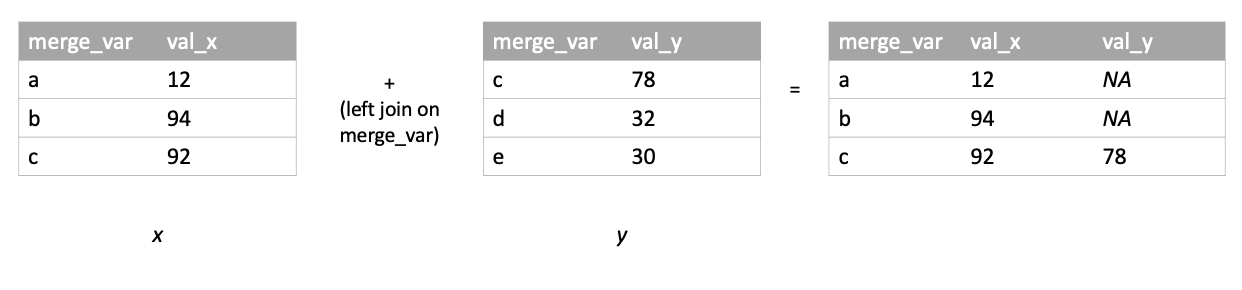
\includegraphics[width=17.25in]{images/left_join}

\hypertarget{python-34}{%
\subsubsection*{Python}\label{python-34}}
\addcontentsline{toc}{subsubsection}{Python}

\begin{Shaded}
\begin{Highlighting}[]
\OperatorTok{\textgreater{}} \ImportTok{import}\NormalTok{ pandas }\ImportTok{as}\NormalTok{ pd}
\OperatorTok{+}\NormalTok{ pd.merge(x, y, how }\OperatorTok{=} \StringTok{\textquotesingle{}left\textquotesingle{}}\NormalTok{)}
\NormalTok{  merge\_var  val\_x  val\_y}
\DecValTok{0}\NormalTok{         a   }\FloatTok{12.0}\NormalTok{    NaN}
\DecValTok{1}\NormalTok{         b   }\FloatTok{94.0}\NormalTok{    NaN}
\DecValTok{2}\NormalTok{         c   }\FloatTok{92.0}   \FloatTok{78.0}
\end{Highlighting}
\end{Shaded}

\hypertarget{r-34}{%
\subsubsection*{R}\label{r-34}}
\addcontentsline{toc}{subsubsection}{R}

\begin{Shaded}
\begin{Highlighting}[]
\SpecialCharTok{\textgreater{}} \CommentTok{\# all.x = T results in a left join}
\ErrorTok{\textgreater{}} \FunctionTok{merge}\NormalTok{(x, y, }\AttributeTok{by =} \StringTok{\textquotesingle{}merge\_var\textquotesingle{}}\NormalTok{, }\AttributeTok{all.x =}\NormalTok{ T)}
\NormalTok{  merge\_var val\_x val\_y}
\DecValTok{1}\NormalTok{         a    }\DecValTok{12}    \ConstantTok{NA}
\DecValTok{2}\NormalTok{         b    }\DecValTok{94}    \ConstantTok{NA}
\DecValTok{3}\NormalTok{         c    }\DecValTok{92}    \DecValTok{78}
\end{Highlighting}
\end{Shaded}

\hypertarget{right-join}{%
\subsection{Right Join}\label{right-join}}

A right join of \emph{x} and \emph{y} keeps all rows of \emph{y} and merges rows of \emph{x} into \emph{y} wherever possible based on the merge criterion:

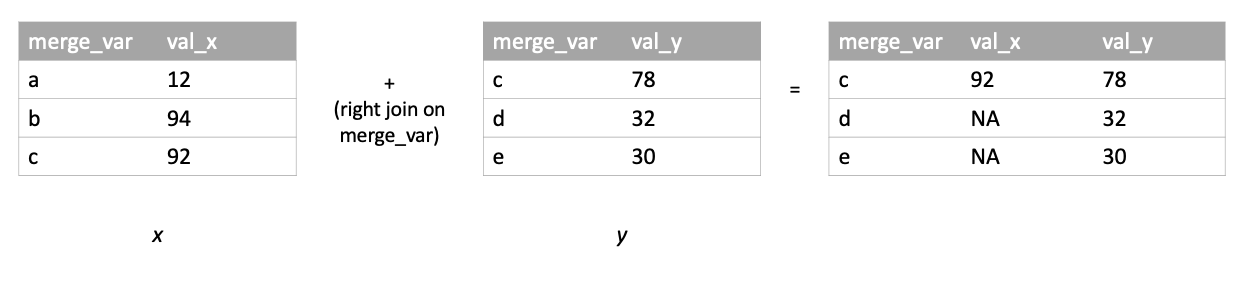
\includegraphics[width=17.25in]{images/right_join}

\hypertarget{python-35}{%
\subsubsection*{Python}\label{python-35}}
\addcontentsline{toc}{subsubsection}{Python}

\begin{Shaded}
\begin{Highlighting}[]
\OperatorTok{\textgreater{}} \ImportTok{import}\NormalTok{ pandas }\ImportTok{as}\NormalTok{ pd}
\OperatorTok{+}\NormalTok{ pd.merge(x, y, how }\OperatorTok{=} \StringTok{\textquotesingle{}right\textquotesingle{}}\NormalTok{)}
\NormalTok{  merge\_var  val\_x  val\_y}
\DecValTok{0}\NormalTok{         c   }\FloatTok{92.0}   \FloatTok{78.0}
\DecValTok{1}\NormalTok{         d    NaN   }\FloatTok{32.0}
\DecValTok{2}\NormalTok{         e    NaN   }\FloatTok{30.0}
\end{Highlighting}
\end{Shaded}

\hypertarget{r-35}{%
\subsubsection*{R}\label{r-35}}
\addcontentsline{toc}{subsubsection}{R}

\begin{Shaded}
\begin{Highlighting}[]
\SpecialCharTok{\textgreater{}} \CommentTok{\# all.y = T results in a right join}
\ErrorTok{\textgreater{}} \FunctionTok{merge}\NormalTok{(x, y, }\AttributeTok{by =} \StringTok{\textquotesingle{}merge\_var\textquotesingle{}}\NormalTok{, }\AttributeTok{all.y =}\NormalTok{ T)}
\NormalTok{  merge\_var val\_x val\_y}
\DecValTok{1}\NormalTok{         c    }\DecValTok{92}    \DecValTok{78}
\DecValTok{2}\NormalTok{         d    }\ConstantTok{NA}    \DecValTok{32}
\DecValTok{3}\NormalTok{         e    }\ConstantTok{NA}    \DecValTok{30}
\end{Highlighting}
\end{Shaded}

\hypertarget{inner-join}{%
\subsection{Inner Join}\label{inner-join}}

An inner join of \emph{x} and \emph{y} returns merged rows for which a match can be found on the merge criterion \emph{in both tables}:

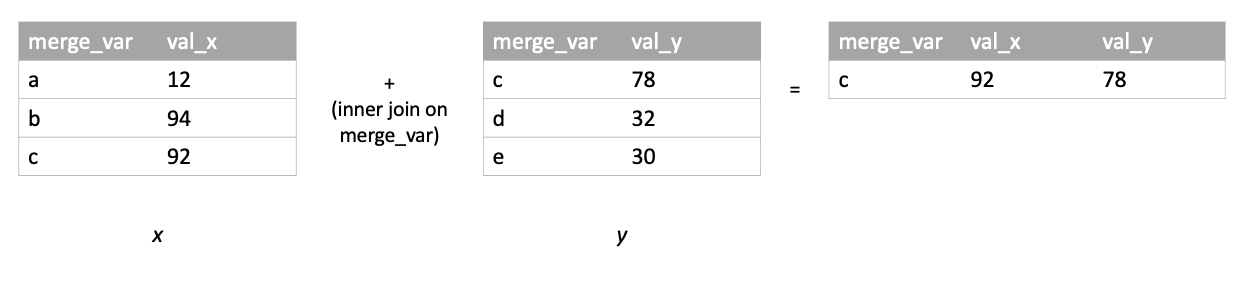
\includegraphics[width=17.25in]{images/inner_join}

\hypertarget{python-36}{%
\subsubsection*{Python}\label{python-36}}
\addcontentsline{toc}{subsubsection}{Python}

\begin{Shaded}
\begin{Highlighting}[]
\OperatorTok{\textgreater{}} \ImportTok{import}\NormalTok{ pandas }\ImportTok{as}\NormalTok{ pd}
\OperatorTok{+}\NormalTok{ pd.merge(x, y, how }\OperatorTok{=} \StringTok{\textquotesingle{}inner\textquotesingle{}}\NormalTok{)}
\NormalTok{  merge\_var  val\_x  val\_y}
\DecValTok{0}\NormalTok{         c   }\FloatTok{92.0}   \FloatTok{78.0}
\end{Highlighting}
\end{Shaded}

\hypertarget{r-36}{%
\subsubsection*{R}\label{r-36}}
\addcontentsline{toc}{subsubsection}{R}

\begin{Shaded}
\begin{Highlighting}[]
\SpecialCharTok{\textgreater{}} \CommentTok{\# with its default arguments, merge() executes an inner join}
\ErrorTok{\textgreater{}} \CommentTok{\# (more specifically, a natural join, which is a kind of}
\ErrorTok{\textgreater{}} \CommentTok{\# inner join in which the merge{-}criterion column is not}
\ErrorTok{\textgreater{}} \CommentTok{\# repeated, despite being initially present in both tables)}
\ErrorTok{\textgreater{}} \FunctionTok{merge}\NormalTok{(x, y, }\AttributeTok{by =} \StringTok{\textquotesingle{}merge\_var\textquotesingle{}}\NormalTok{)}
\NormalTok{  merge\_var val\_x val\_y}
\DecValTok{1}\NormalTok{         c    }\DecValTok{92}    \DecValTok{78}
\end{Highlighting}
\end{Shaded}

\hypertarget{outer-join}{%
\subsection{Outer Join}\label{outer-join}}

An outer join of \emph{x} and \emph{y} keeps all rows from both tables, merging rows wherever possible based on the merge criterion:

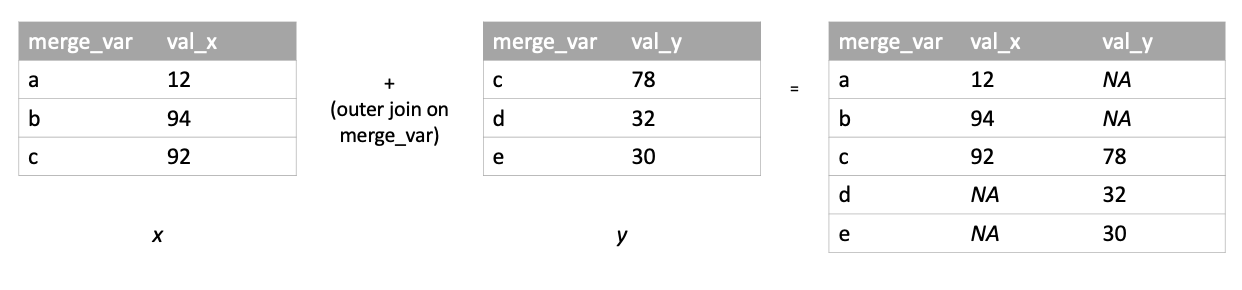
\includegraphics[width=17.25in]{images/outer_join}

\hypertarget{python-37}{%
\subsubsection*{Python}\label{python-37}}
\addcontentsline{toc}{subsubsection}{Python}

\begin{Shaded}
\begin{Highlighting}[]
\OperatorTok{\textgreater{}} \ImportTok{import}\NormalTok{ pandas }\ImportTok{as}\NormalTok{ pd}
\OperatorTok{+}\NormalTok{ pd.merge(x, y, how }\OperatorTok{=} \StringTok{\textquotesingle{}outer\textquotesingle{}}\NormalTok{)}
\NormalTok{  merge\_var  val\_x  val\_y}
\DecValTok{0}\NormalTok{         a   }\FloatTok{12.0}\NormalTok{    NaN}
\DecValTok{1}\NormalTok{         b   }\FloatTok{94.0}\NormalTok{    NaN}
\DecValTok{2}\NormalTok{         c   }\FloatTok{92.0}   \FloatTok{78.0}
\DecValTok{3}\NormalTok{         d    NaN   }\FloatTok{32.0}
\DecValTok{4}\NormalTok{         e    NaN   }\FloatTok{30.0}
\end{Highlighting}
\end{Shaded}

\hypertarget{r-37}{%
\subsubsection*{R}\label{r-37}}
\addcontentsline{toc}{subsubsection}{R}

\begin{Shaded}
\begin{Highlighting}[]
\SpecialCharTok{\textgreater{}} \CommentTok{\# all = T (or all.x = T AND all.y = T) results in an outer join}
\ErrorTok{\textgreater{}} \FunctionTok{merge}\NormalTok{(x, y, }\AttributeTok{by =} \StringTok{\textquotesingle{}merge\_var\textquotesingle{}}\NormalTok{, }\AttributeTok{all =}\NormalTok{ T)}
\NormalTok{  merge\_var val\_x val\_y}
\DecValTok{1}\NormalTok{         a    }\DecValTok{12}    \ConstantTok{NA}
\DecValTok{2}\NormalTok{         b    }\DecValTok{94}    \ConstantTok{NA}
\DecValTok{3}\NormalTok{         c    }\DecValTok{92}    \DecValTok{78}
\DecValTok{4}\NormalTok{         d    }\ConstantTok{NA}    \DecValTok{32}
\DecValTok{5}\NormalTok{         e    }\ConstantTok{NA}    \DecValTok{30}
\end{Highlighting}
\end{Shaded}

\hypertarget{aggregation-and-group-operations}{%
\chapter{Aggregation and Group Operations}\label{aggregation-and-group-operations}}

This chapter looks at manipulating and summarizing data by groups.

\hypertarget{cross-tabulation}{%
\section{Cross tabulation}\label{cross-tabulation}}

Cross tabulation is the process of determining frequencies per group (or determining values based on frequencies, like proportions), with groups delineated by one or more variables (e.g., nationality and sex).

The Python and R examples of cross tabulation below both make use of the following dataset, \texttt{dat}:

\begin{Shaded}
\begin{Highlighting}[]
\SpecialCharTok{\textgreater{}}\NormalTok{ dat}
\NormalTok{  nationality sex}
\DecValTok{1}\NormalTok{    Canadian   m}
\DecValTok{2}\NormalTok{      French   f}
\DecValTok{3}\NormalTok{      French   f}
\DecValTok{4}\NormalTok{    Egyptian   m}
\DecValTok{5}\NormalTok{    Canadian   f}
\end{Highlighting}
\end{Shaded}

\hypertarget{python-38}{%
\subsubsection*{Python}\label{python-38}}
\addcontentsline{toc}{subsubsection}{Python}

The \textbf{pandas} package contains a \texttt{crosstab()} function for cross tabulation with two or more variables. Alternatively, the \texttt{groupby()} function, also in \textbf{pandas}, facilitates cross tabulation by one or more variables when used in combination with \texttt{count()}.

\begin{Shaded}
\begin{Highlighting}[]
\OperatorTok{\textgreater{}} \ImportTok{import}\NormalTok{ pandas }\ImportTok{as}\NormalTok{ pd}
\OperatorTok{+}\NormalTok{ pd.crosstab(dat.nationality, dat.sex)}
\NormalTok{sex          f  m}
\NormalTok{nationality      }
\NormalTok{Canadian     }\DecValTok{1}  \DecValTok{1}
\NormalTok{Egyptian     }\DecValTok{0}  \DecValTok{1}
\NormalTok{French       }\DecValTok{2}  \DecValTok{0}
\OperatorTok{\textgreater{}}\NormalTok{ dat.groupby(by }\OperatorTok{=} \StringTok{\textquotesingle{}nationality\textquotesingle{}}\NormalTok{).nationality.count()}
\NormalTok{nationality}
\NormalTok{Canadian    }\DecValTok{2}
\NormalTok{Egyptian    }\DecValTok{1}
\NormalTok{French      }\DecValTok{2}
\NormalTok{Name: nationality, dtype: int64}
\OperatorTok{\textgreater{}}\NormalTok{ dat.groupby(by }\OperatorTok{=}\NormalTok{ [}\StringTok{\textquotesingle{}nationality\textquotesingle{}}\NormalTok{, }\StringTok{\textquotesingle{}sex\textquotesingle{}}\NormalTok{]).nationality.count()}
\OperatorTok{+} \CommentTok{\# Or: dat.groupby(by = [\textquotesingle{}nationality\textquotesingle{}, \textquotesingle{}sex\textquotesingle{}]).sex.count()}
\NormalTok{nationality  sex}
\NormalTok{Canadian     f      }\DecValTok{1}
\NormalTok{             m      }\DecValTok{1}
\NormalTok{Egyptian     m      }\DecValTok{1}
\NormalTok{French       f      }\DecValTok{2}
\NormalTok{Name: nationality, dtype: int64}
\end{Highlighting}
\end{Shaded}

\hypertarget{r-38}{%
\subsubsection*{R}\label{r-38}}
\addcontentsline{toc}{subsubsection}{R}

The \texttt{table()} function performs cross tabulation in R. A user can enter a single grouping variable or enter multiple grouping variables separated by a comma(s). The \texttt{xtabs()} function also computes cross-tabs; a user enters the variables to be used for grouping in formula notation.

\begin{Shaded}
\begin{Highlighting}[]
\SpecialCharTok{\textgreater{}} \FunctionTok{table}\NormalTok{(dat}\SpecialCharTok{$}\NormalTok{nationality)}

\NormalTok{Canadian Egyptian   French }
       \DecValTok{2}        \DecValTok{1}        \DecValTok{2} 
\SpecialCharTok{\textgreater{}} \FunctionTok{table}\NormalTok{(dat}\SpecialCharTok{$}\NormalTok{nationality, dat}\SpecialCharTok{$}\NormalTok{sex)}
          
\NormalTok{           f m}
\NormalTok{  Canadian }\DecValTok{1} \DecValTok{1}
\NormalTok{  Egyptian }\DecValTok{0} \DecValTok{1}
\NormalTok{  French   }\DecValTok{2} \DecValTok{0}
\SpecialCharTok{\textgreater{}} \FunctionTok{xtabs}\NormalTok{(}\AttributeTok{formula =} \SpecialCharTok{\textasciitilde{}}\NormalTok{nationality }\SpecialCharTok{+}\NormalTok{ sex, }\AttributeTok{data =}\NormalTok{ dat)}
\NormalTok{           sex}
\NormalTok{nationality f m}
\NormalTok{   Canadian }\DecValTok{1} \DecValTok{1}
\NormalTok{   Egyptian }\DecValTok{0} \DecValTok{1}
\NormalTok{   French   }\DecValTok{2} \DecValTok{0}
\end{Highlighting}
\end{Shaded}

\hypertarget{group-summaries}{%
\section{Group summaries}\label{group-summaries}}

Computing statistical summaries per group.

\hypertarget{python-39}{%
\subsubsection*{Python}\label{python-39}}
\addcontentsline{toc}{subsubsection}{Python}

The \texttt{groupby()} function from \textbf{Pandas} splits up a data set based on one or more grouping variables. Summarizing functions---like \texttt{mean()}, \texttt{sum()}, and so on---can then be applied to those groups. In the first example below, we use \texttt{groupby()} to group rows of the \texttt{mtcars} dataset by the number of cylinders each car has; from there, we select just the \texttt{mpg} column and call \texttt{mean()}, thus producing the average miles per gallon within each cylinder group. In the second example, we again group observations by \texttt{cyl}, but instead of then selecting just the \texttt{mpg} column, we directly call \texttt{mean()}; this gives the mean for each variable in the data set within each cylinder group. Finally, in the third example, we group by two variables---\texttt{cyl} and \texttt{vs}---and then use the \texttt{describe()} function to generate a set of descriptive statistics for \texttt{mpg} within each \texttt{cylinder}*\texttt{vs} group (e.g., mean, SD, minimum, etc.).

\begin{Shaded}
\begin{Highlighting}[]
\OperatorTok{\textgreater{}} \ImportTok{import}\NormalTok{ pandas }\ImportTok{as}\NormalTok{ pd}
\OperatorTok{+} 
\OperatorTok{+}\NormalTok{ mean\_mpg\_by\_cyl }\OperatorTok{=}\NormalTok{ mtcars.groupby(by }\OperatorTok{=} \StringTok{\textquotesingle{}cyl\textquotesingle{}}\NormalTok{)[}\StringTok{\textquotesingle{}mpg\textquotesingle{}}\NormalTok{].mean()}
\OperatorTok{+} \BuiltInTok{print}\NormalTok{(mean\_mpg\_by\_cyl)}
\NormalTok{cyl}
\FloatTok{4.0}    \FloatTok{26.663636}
\FloatTok{6.0}    \FloatTok{19.742857}
\FloatTok{8.0}    \FloatTok{15.100000}
\NormalTok{Name: mpg, dtype: float64}
\OperatorTok{\textgreater{}}\NormalTok{ means\_all\_vars }\OperatorTok{=}\NormalTok{ mtcars.groupby(by }\OperatorTok{=} \StringTok{\textquotesingle{}cyl\textquotesingle{}}\NormalTok{).mean()}
\OperatorTok{+} \BuiltInTok{print}\NormalTok{(means\_all\_vars)}
\NormalTok{           mpg        disp          hp  ...        am      gear      carb}
\NormalTok{cyl                                     ...                              }
\FloatTok{4.0}  \FloatTok{26.663636}  \FloatTok{105.136364}   \FloatTok{82.636364}\NormalTok{  ...  }\FloatTok{0.727273}  \FloatTok{4.090909}  \FloatTok{1.545455}
\FloatTok{6.0}  \FloatTok{19.742857}  \FloatTok{183.314286}  \FloatTok{122.285714}\NormalTok{  ...  }\FloatTok{0.428571}  \FloatTok{3.857143}  \FloatTok{3.428571}
\FloatTok{8.0}  \FloatTok{15.100000}  \FloatTok{353.100000}  \FloatTok{209.214286}\NormalTok{  ...  }\FloatTok{0.142857}  \FloatTok{3.285714}  \FloatTok{3.500000}

\NormalTok{[}\DecValTok{3}\NormalTok{ rows x }\DecValTok{10}\NormalTok{ columns]}
\OperatorTok{\textgreater{}}\NormalTok{ mpg\_by\_cyl\_vs }\OperatorTok{=}\NormalTok{ mtcars.groupby(by }\OperatorTok{=}\NormalTok{ [}\StringTok{\textquotesingle{}cyl\textquotesingle{}}\NormalTok{, }\StringTok{\textquotesingle{}vs\textquotesingle{}}\NormalTok{])[}\StringTok{\textquotesingle{}mpg\textquotesingle{}}\NormalTok{].describe()}
\OperatorTok{+} \BuiltInTok{print}\NormalTok{(mpg\_by\_cyl\_vs)}
\NormalTok{         count       mean       std   }\BuiltInTok{min}     \DecValTok{25}\OperatorTok{\%}    \DecValTok{50}\OperatorTok{\%}    \DecValTok{75}\OperatorTok{\%}   \BuiltInTok{max}
\NormalTok{cyl vs                                                               }
\FloatTok{4.0} \FloatTok{0.0}    \FloatTok{1.0}  \FloatTok{26.000000}\NormalTok{       NaN  }\FloatTok{26.0}  \FloatTok{26.000}  \FloatTok{26.00}  \FloatTok{26.00}  \FloatTok{26.0}
    \FloatTok{1.0}   \FloatTok{10.0}  \FloatTok{26.730000}  \FloatTok{4.748111}  \FloatTok{21.4}  \FloatTok{22.800}  \FloatTok{25.85}  \FloatTok{30.40}  \FloatTok{33.9}
\FloatTok{6.0} \FloatTok{0.0}    \FloatTok{3.0}  \FloatTok{20.566667}  \FloatTok{0.750555}  \FloatTok{19.7}  \FloatTok{20.350}  \FloatTok{21.00}  \FloatTok{21.00}  \FloatTok{21.0}
    \FloatTok{1.0}    \FloatTok{4.0}  \FloatTok{19.125000}  \FloatTok{1.631717}  \FloatTok{17.8}  \FloatTok{18.025}  \FloatTok{18.65}  \FloatTok{19.75}  \FloatTok{21.4}
\FloatTok{8.0} \FloatTok{0.0}   \FloatTok{14.0}  \FloatTok{15.100000}  \FloatTok{2.560048}  \FloatTok{10.4}  \FloatTok{14.400}  \FloatTok{15.20}  \FloatTok{16.25}  \FloatTok{19.2}
\end{Highlighting}
\end{Shaded}

\hypertarget{r-39}{%
\subsubsection*{R}\label{r-39}}
\addcontentsline{toc}{subsubsection}{R}

The \texttt{aggregate()} function can be used to generate by-group statistical summaries based on one or more grouping variables. Grouping variables can be declared as a list in the function's \texttt{by} argument. Alternatively, the grouping variable(s) and the variable to be summarized can be passed to \texttt{aggregate()} in formula notation: \texttt{var\_to\_be\_aggregated\ \textasciitilde{}\ grouping\_var\_1\ +\ ...\ +\ grouping\_var\_N}. The summarizing function (e.g., \texttt{mean()}; \texttt{median()}; etc.) is declared in the \texttt{FUN} argument.

\begin{Shaded}
\begin{Highlighting}[]
\SpecialCharTok{\textgreater{}} \CommentTok{\# One grouping variable}
\ErrorTok{\textgreater{}} \CommentTok{\# Calculating mean of \textasciigrave{}mpg\textasciigrave{} in each \textasciigrave{}cyl\textasciigrave{} group}
\ErrorTok{\textgreater{}} \FunctionTok{aggregate}\NormalTok{(}\AttributeTok{x =}\NormalTok{ mtcars}\SpecialCharTok{$}\NormalTok{mpg, }
\SpecialCharTok{+}           \AttributeTok{by =} \FunctionTok{list}\NormalTok{(}\AttributeTok{cyl =}\NormalTok{ mtcars}\SpecialCharTok{$}\NormalTok{cyl), }
\SpecialCharTok{+}           \AttributeTok{FUN =} \StringTok{"mean"}\NormalTok{) }
\NormalTok{  cyl        x}
\DecValTok{1}   \DecValTok{4} \FloatTok{26.66364}
\DecValTok{2}   \DecValTok{6} \FloatTok{19.74286}
\DecValTok{3}   \DecValTok{8} \FloatTok{15.10000}
\end{Highlighting}
\end{Shaded}

Adding \texttt{drop=FALSE} ensures all combinations of levels are returned even if no data exist at that combination. Below the final row is \texttt{NA} since there are no 8-cylinder cars with a ``straight'' engine (vs = 1).

\begin{Shaded}
\begin{Highlighting}[]
\SpecialCharTok{\textgreater{}} \CommentTok{\# Two or more grouping variables}
\ErrorTok{\textgreater{}} \CommentTok{\# Calculating max of \textasciigrave{}mpg\textasciigrave{} in each \textasciigrave{}cyl\textasciigrave{}*\textasciigrave{}vs\textasciigrave{} group}
\ErrorTok{\textgreater{}} \FunctionTok{aggregate}\NormalTok{(}\AttributeTok{x =}\NormalTok{ mtcars}\SpecialCharTok{$}\NormalTok{mpg, }
\SpecialCharTok{+}           \AttributeTok{by =} \FunctionTok{list}\NormalTok{(}\AttributeTok{cyl =}\NormalTok{ mtcars}\SpecialCharTok{$}\NormalTok{cyl, }\AttributeTok{vs =}\NormalTok{ mtcars}\SpecialCharTok{$}\NormalTok{vs), }
\SpecialCharTok{+}           \AttributeTok{FUN =} \StringTok{"max"}\NormalTok{, }\AttributeTok{drop =} \ConstantTok{FALSE}\NormalTok{) }
\NormalTok{  cyl vs    x}
\DecValTok{1}   \DecValTok{4}  \DecValTok{0} \FloatTok{26.0}
\DecValTok{2}   \DecValTok{6}  \DecValTok{0} \FloatTok{21.0}
\DecValTok{3}   \DecValTok{8}  \DecValTok{0} \FloatTok{19.2}
\DecValTok{4}   \DecValTok{4}  \DecValTok{1} \FloatTok{33.9}
\DecValTok{5}   \DecValTok{6}  \DecValTok{1} \FloatTok{21.4}
\DecValTok{6}   \DecValTok{8}  \DecValTok{1}   \ConstantTok{NA}
\end{Highlighting}
\end{Shaded}

\begin{Shaded}
\begin{Highlighting}[]
\SpecialCharTok{\textgreater{}} \CommentTok{\# Or, specify the variable to summarize and the grouping variables in formula notation}
\ErrorTok{\textgreater{}} \FunctionTok{aggregate}\NormalTok{(mpg }\SpecialCharTok{\textasciitilde{}}\NormalTok{ cyl }\SpecialCharTok{+}\NormalTok{ vs, }\AttributeTok{data =}\NormalTok{ mtcars, }\AttributeTok{FUN =}\NormalTok{ max)}
\end{Highlighting}
\end{Shaded}

The \textbf{tidyverse} also offers a summarizing function, \texttt{summarize()} (or \texttt{summarise()}, for the Britons), which is in the \textbf{dplyr} package. After grouping a data frame/tibble (with, e.g., \textbf{dplyr}'s \texttt{group\_by()} function), a user passes it to \texttt{summarize()}, specifying in the function call how the summary statistic should be calculated.

\begin{Shaded}
\begin{Highlighting}[]
\SpecialCharTok{\textgreater{}} \FunctionTok{library}\NormalTok{(dplyr)}
\SpecialCharTok{\textgreater{}}\NormalTok{ mtcars }\SpecialCharTok{\%\textgreater{}\%} 
\SpecialCharTok{+}   \FunctionTok{group\_by}\NormalTok{(cyl, vs) }\SpecialCharTok{\%\textgreater{}\%} 
\SpecialCharTok{+}   \FunctionTok{summarize}\NormalTok{(}\AttributeTok{avg\_mpg =} \FunctionTok{mean}\NormalTok{(mpg))}
\StringTok{\textasciigrave{}}\AttributeTok{summarise()}\StringTok{\textasciigrave{}}\NormalTok{ has grouped output by }\StringTok{\textquotesingle{}cyl\textquotesingle{}}\NormalTok{. You can override using the }\StringTok{\textasciigrave{}}\AttributeTok{.groups}\StringTok{\textasciigrave{}}
\NormalTok{argument.}
\CommentTok{\# A tibble: 5 x 3}
\CommentTok{\# Groups:   cyl [3]}
\NormalTok{    cyl    vs avg\_mpg}
  \SpecialCharTok{\textless{}}\NormalTok{dbl}\SpecialCharTok{\textgreater{}} \ErrorTok{\textless{}}\NormalTok{dbl}\SpecialCharTok{\textgreater{}}   \ErrorTok{\textless{}}\NormalTok{dbl}\SpecialCharTok{\textgreater{}}
\DecValTok{1}     \DecValTok{4}     \DecValTok{0}    \DecValTok{26}  
\DecValTok{2}     \DecValTok{4}     \DecValTok{1}    \FloatTok{26.7}
\DecValTok{3}     \DecValTok{6}     \DecValTok{0}    \FloatTok{20.6}
\DecValTok{4}     \DecValTok{6}     \DecValTok{1}    \FloatTok{19.1}
\DecValTok{5}     \DecValTok{8}     \DecValTok{0}    \FloatTok{15.1}
\end{Highlighting}
\end{Shaded}

\texttt{summarize()} makes it easy to specify relatively complicated summary calculations without needing to write an external function.

\begin{Shaded}
\begin{Highlighting}[]
\SpecialCharTok{\textgreater{}}\NormalTok{ mtcars }\SpecialCharTok{\%\textgreater{}\%} 
\SpecialCharTok{+}   \FunctionTok{group\_by}\NormalTok{(cyl, vs) }\SpecialCharTok{\%\textgreater{}\%} 
\SpecialCharTok{+}   \FunctionTok{summarize}\NormalTok{(}\AttributeTok{avg\_mpg =} \FunctionTok{mean}\NormalTok{(mpg),}
\SpecialCharTok{+}             \AttributeTok{complicated\_summary\_calculation =} 
\SpecialCharTok{+}               \FunctionTok{min}\NormalTok{(mpg)}\SpecialCharTok{\^{}}\FloatTok{0.5} \SpecialCharTok{*} 
\SpecialCharTok{+}               \FunctionTok{mean}\NormalTok{(wt)}\SpecialCharTok{\^{}}\FloatTok{0.5} \SpecialCharTok{+} 
\SpecialCharTok{+}               \FunctionTok{mean}\NormalTok{(disp)}\SpecialCharTok{\^{}}\NormalTok{(}\DecValTok{1}\SpecialCharTok{/}\FunctionTok{mean}\NormalTok{(hp)))}
\StringTok{\textasciigrave{}}\AttributeTok{summarise()}\StringTok{\textasciigrave{}}\NormalTok{ has grouped output by }\StringTok{\textquotesingle{}cyl\textquotesingle{}}\NormalTok{. You can override using the }\StringTok{\textasciigrave{}}\AttributeTok{.groups}\StringTok{\textasciigrave{}}
\NormalTok{argument.}
\CommentTok{\# A tibble: 5 x 4}
\CommentTok{\# Groups:   cyl [3]}
\NormalTok{    cyl    vs avg\_mpg complicated\_summary\_calculation}
  \SpecialCharTok{\textless{}}\NormalTok{dbl}\SpecialCharTok{\textgreater{}} \ErrorTok{\textless{}}\NormalTok{dbl}\SpecialCharTok{\textgreater{}}   \ErrorTok{\textless{}}\NormalTok{dbl}\SpecialCharTok{\textgreater{}}                           \ErrorTok{\textless{}}\NormalTok{dbl}\SpecialCharTok{\textgreater{}}
\DecValTok{1}     \DecValTok{4}     \DecValTok{0}    \DecValTok{26}                              \FloatTok{8.51}
\DecValTok{2}     \DecValTok{4}     \DecValTok{1}    \FloatTok{26.7}                            \FloatTok{8.07}
\DecValTok{3}     \DecValTok{6}     \DecValTok{0}    \FloatTok{20.6}                            \FloatTok{8.41}
\DecValTok{4}     \DecValTok{6}     \DecValTok{1}    \FloatTok{19.1}                            \FloatTok{8.81}
\DecValTok{5}     \DecValTok{8}     \DecValTok{0}    \FloatTok{15.1}                            \FloatTok{7.48}
\end{Highlighting}
\end{Shaded}

\hypertarget{centering-and-scaling}{%
\section{Centering and Scaling}\label{centering-and-scaling}}

\emph{Centering} refers to subtracting a constant, such as the mean, from every one of set of values. This is sometimes performed to aid interpretation of linear model coefficients.

\emph{Scaling} refers to rescaling a column or vector of values such that their mean is zero and their standard deviation is one. This is sometimes performed to put multiple variables on the same scale and is often recommended for procedures such as principal components analysis (PCA).

\hypertarget{python-40}{%
\subsubsection*{Python}\label{python-40}}
\addcontentsline{toc}{subsubsection}{Python}

The \texttt{scale()} function from the \textbf{preprocessing} module of the \textbf{scikit-learn} package provides one-step centering and scaling. To center a variable at zero without scaling it, use \texttt{scale()} with \texttt{with\_mean\ =\ True} and \texttt{with\_std\ =\ False} (both are \texttt{True} by default).

\begin{Shaded}
\begin{Highlighting}[]
\OperatorTok{\textgreater{}} \ImportTok{from}\NormalTok{ sklearn }\ImportTok{import}\NormalTok{ preprocessing}
\OperatorTok{+} 
\OperatorTok{+}\NormalTok{ centered\_mpg }\OperatorTok{=}\NormalTok{ preprocessing.scale(mtcars.mpg, with\_mean }\OperatorTok{=} \VariableTok{True}\NormalTok{, with\_std }\OperatorTok{=} \VariableTok{False}\NormalTok{)}
\OperatorTok{+}\NormalTok{ centered\_mpg.mean()}
\OperatorTok{{-}}\FloatTok{3.1086244689504383e{-}15}
\end{Highlighting}
\end{Shaded}

To scale a variable after centering it (so that its mean is zero and its standard deviation is one), use \texttt{scale()} with \texttt{with\_mean\ =\ True} and \texttt{with\_std\ =\ True}.

\begin{Shaded}
\begin{Highlighting}[]
\OperatorTok{\textgreater{}} \ImportTok{from}\NormalTok{ sklearn }\ImportTok{import}\NormalTok{ preprocessing}
\OperatorTok{+} 
\OperatorTok{+}\NormalTok{ scaled\_mpg }\OperatorTok{=}\NormalTok{ preprocessing.scale(mtcars.mpg, with\_mean }\OperatorTok{=} \VariableTok{True}\NormalTok{, with\_std }\OperatorTok{=} \VariableTok{True}\NormalTok{)}
\OperatorTok{+}\NormalTok{ scaled\_mpg.mean()}
\OperatorTok{{-}}\FloatTok{4.996003610813204e{-}16}
\OperatorTok{\textgreater{}}\NormalTok{ scaled\_mpg.std()}
\FloatTok{1.0}
\end{Highlighting}
\end{Shaded}

\hypertarget{r-40}{%
\subsubsection*{R}\label{r-40}}
\addcontentsline{toc}{subsubsection}{R}

The \texttt{scale()} function can both center and scale variables.

To center a variable without scaling it, call \texttt{scale()} with the \texttt{center} argument set to \texttt{TRUE} and the \texttt{scale} argument set to \texttt{FALSE}. The variable's mean will be subtracted off of each of the variable values. (Note: If desired, the \texttt{center} argument can be set to a numeric value instead of \texttt{TRUE}/\texttt{FALSE}; in that case, each variable value will have the argument value subtracted off of it.)

\begin{Shaded}
\begin{Highlighting}[]
\SpecialCharTok{\textgreater{}}\NormalTok{ centered\_mpg }\OtherTok{\textless{}{-}} \FunctionTok{scale}\NormalTok{(mtcars}\SpecialCharTok{$}\NormalTok{mpg, }\AttributeTok{center =}\NormalTok{ T, }\AttributeTok{scale =}\NormalTok{ F)}
\SpecialCharTok{\textgreater{}} \FunctionTok{mean}\NormalTok{(centered\_mpg)}
\NormalTok{[}\DecValTok{1}\NormalTok{] }\FloatTok{4.440892e{-}16}
\end{Highlighting}
\end{Shaded}

To scale a variable (while also centering it), call \texttt{scale()} with the \texttt{center} and \texttt{scale} arguments set to \texttt{TRUE} (these are the default argument values). The variable's mean will be subtracted off of each of the variable values, and each value will then be divided by the variable's standard deviation. (Note: As with the \texttt{center} argument, the \texttt{scale} argument can also be set to a numeric value instead of \texttt{TRUE}/\texttt{FALSE}; in that case, the divisor will be the argument value instead of the standard deviation.)

\begin{Shaded}
\begin{Highlighting}[]
\SpecialCharTok{\textgreater{}}\NormalTok{ scaled\_mpg }\OtherTok{\textless{}{-}} \FunctionTok{scale}\NormalTok{(mtcars}\SpecialCharTok{$}\NormalTok{mpg, }\AttributeTok{center =}\NormalTok{ T, }\AttributeTok{scale =}\NormalTok{ T)}
\SpecialCharTok{\textgreater{}} \FunctionTok{mean}\NormalTok{(scaled\_mpg)}
\NormalTok{[}\DecValTok{1}\NormalTok{] }\FloatTok{7.112366e{-}17}
\SpecialCharTok{\textgreater{}} \FunctionTok{sd}\NormalTok{(scaled\_mpg)}
\NormalTok{[}\DecValTok{1}\NormalTok{] }\DecValTok{1}
\end{Highlighting}
\end{Shaded}

\hypertarget{basic-plotting-and-visualization}{%
\chapter{Basic Plotting and Visualization}\label{basic-plotting-and-visualization}}

This chapter looks at creating basic plots to explore and understand data. Visualization in Python and R is a gigantic and evolving topic. We don't pretend to present a comprehensive comparison.

The plots below make use of the \href{https://allisonhorst.github.io/palmerpenguins/}{\textbf{palmerpenguins}} data set, which contains various measurements for 344 penguins across three islands in the Antarctic Palmer Archipelago. The data were collected by \href{https://www.uaf.edu/cfos/people/faculty/detail/kristen-gorman.php}{Kristen Gorman} and colleagues, and they were made available under a \href{https://creativecommons.org/share-your-work/public-domain/cc0/}{CC0 public domain license} by Allison Horst, Alison Hill, and Kristen Gorman.

For the R sections below, we discuss how to generate plots using base R and using \textbf{ggplot2}.

Here's a glimpse at the data set:

\begin{Shaded}
\begin{Highlighting}[]
\SpecialCharTok{\textgreater{}} \FunctionTok{head}\NormalTok{(penguins)}
\CommentTok{\# A tibble: 6 x 8}
\NormalTok{  species island bill\_length\_mm bill\_depth\_mm flipper\_length\_}\SpecialCharTok{\textasciitilde{}}\NormalTok{ body\_mass\_g sex  }
  \SpecialCharTok{\textless{}}\NormalTok{fct}\SpecialCharTok{\textgreater{}}   \ErrorTok{\textless{}}\NormalTok{fct}\SpecialCharTok{\textgreater{}}           \ErrorTok{\textless{}}\NormalTok{dbl}\SpecialCharTok{\textgreater{}}         \ErrorTok{\textless{}}\NormalTok{dbl}\SpecialCharTok{\textgreater{}}            \ErrorTok{\textless{}}\NormalTok{int}\SpecialCharTok{\textgreater{}}       \ErrorTok{\textless{}}\NormalTok{int}\SpecialCharTok{\textgreater{}} \ErrorTok{\textless{}}\NormalTok{fct}\SpecialCharTok{\textgreater{}}
\DecValTok{1}\NormalTok{ Adelie  Torge}\SpecialCharTok{\textasciitilde{}}           \FloatTok{39.1}          \FloatTok{18.7}              \DecValTok{181}        \DecValTok{3750}\NormalTok{ male }
\DecValTok{2}\NormalTok{ Adelie  Torge}\SpecialCharTok{\textasciitilde{}}           \FloatTok{39.5}          \FloatTok{17.4}              \DecValTok{186}        \DecValTok{3800}\NormalTok{ fema}\SpecialCharTok{\textasciitilde{}}
\DecValTok{3}\NormalTok{ Adelie  Torge}\SpecialCharTok{\textasciitilde{}}           \FloatTok{40.3}          \DecValTok{18}                \DecValTok{195}        \DecValTok{3250}\NormalTok{ fema}\SpecialCharTok{\textasciitilde{}}
\DecValTok{4}\NormalTok{ Adelie  Torge}\SpecialCharTok{\textasciitilde{}}           \ConstantTok{NA}            \ConstantTok{NA}                 \ConstantTok{NA}          \ConstantTok{NA} \SpecialCharTok{\textless{}}\ConstantTok{NA}\SpecialCharTok{\textgreater{}} 
\DecValTok{5}\NormalTok{ Adelie  Torge}\SpecialCharTok{\textasciitilde{}}           \FloatTok{36.7}          \FloatTok{19.3}              \DecValTok{193}        \DecValTok{3450}\NormalTok{ fema}\SpecialCharTok{\textasciitilde{}}
\DecValTok{6}\NormalTok{ Adelie  Torge}\SpecialCharTok{\textasciitilde{}}           \FloatTok{39.3}          \FloatTok{20.6}              \DecValTok{190}        \DecValTok{3650}\NormalTok{ male }
\CommentTok{\# ... with 1 more variable: year \textless{}int\textgreater{}}
\end{Highlighting}
\end{Shaded}

\hypertarget{histograms}{%
\section{Histograms}\label{histograms}}

Visualizing the distribution of numeric data.

\hypertarget{python-41}{%
\subsubsection*{Python}\label{python-41}}
\addcontentsline{toc}{subsubsection}{Python}

The Python plotting library Matplotlib's \texttt{hist()} function computes and plots a histogram. There are many parameters that can be specified within the \texttt{hist()} function so that you can customize the output histogram plot to best fit your needs. Some parameters include the number of bins, the upper and lower bounds on each bin, weights, colors, and more.

Below we show a histogram of the bill length from the dataset. We specified 30 bins each of which is light blue with a black outline of linewidth 1. The \texttt{hist()} defaults to no outline which can make it difficult to distinguish bins clearly, so we add in the bin outlines here.

One thing to note is that the bins are left inclusive and right exclusive. For example, if a particular bin spans the range of 1 to 3, the bin will include the value 1 but will exclude the value 2 (and will include all values between 1 and 3). In short, bin ranges are as follows {[}x1,x2) where x1 is the starting point of the bin and x2 is the ending point of the bin.

Notice the semicolon at the end of the \texttt{plt.hist()} function. This suppresses the printing of the array generated to create the histogram.

\begin{Shaded}
\begin{Highlighting}[]
\OperatorTok{\textgreater{}} \ImportTok{import}\NormalTok{ matplotlib.pyplot }\ImportTok{as}\NormalTok{ plt}
\OperatorTok{+} 
\OperatorTok{+}\NormalTok{ plt.clf()}
\OperatorTok{+}\NormalTok{ plt.hist(penguins.bill\_length\_mm, bins}\OperatorTok{=}\DecValTok{30}\NormalTok{, }\BuiltInTok{range}\OperatorTok{=}\NormalTok{(}\DecValTok{30}\NormalTok{,}\DecValTok{60}\NormalTok{),}
\OperatorTok{+}\NormalTok{          color}\OperatorTok{=}\StringTok{\textquotesingle{}lightblue\textquotesingle{}}\NormalTok{, edgecolor}\OperatorTok{=}\StringTok{\textquotesingle{}k\textquotesingle{}}\NormalTok{, linewidth}\OperatorTok{=}\DecValTok{1}\NormalTok{)}\OperatorTok{;}
\OperatorTok{+}\NormalTok{ plt.title(}\StringTok{"Penguin Bill Lengths"}\NormalTok{)}
\OperatorTok{+}\NormalTok{ plt.xlabel(}\StringTok{"Bill Length (mm)"}\NormalTok{)}
\OperatorTok{+}\NormalTok{ plt.ylabel(}\StringTok{"Count"}\NormalTok{)}
\OperatorTok{+}\NormalTok{ plt.show()}
\end{Highlighting}
\end{Shaded}

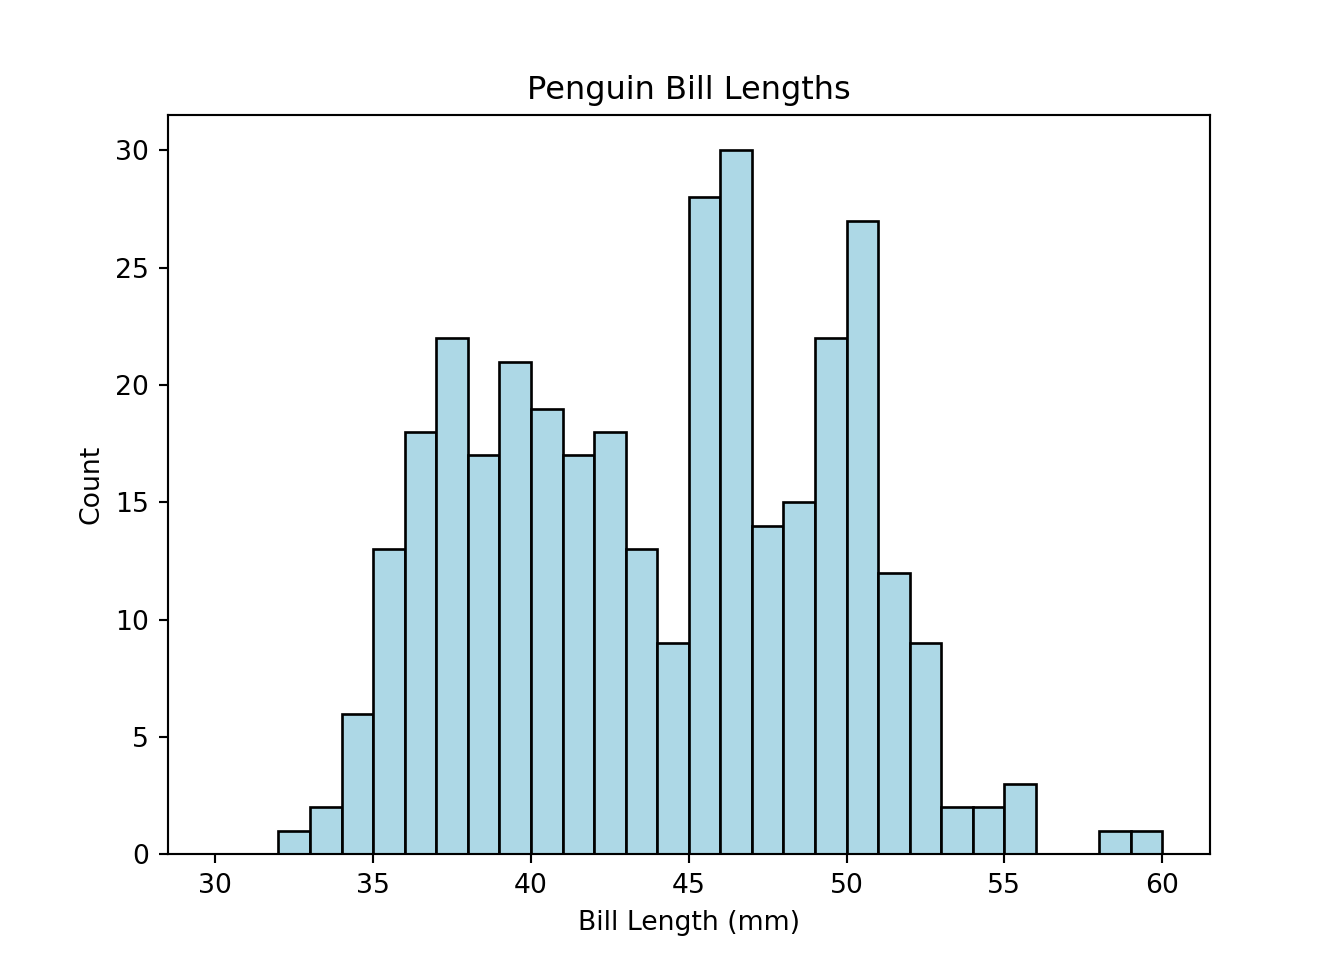
\includegraphics{_main_files/figure-latex/unnamed-chunk-269-1.pdf}

\hypertarget{r-41}{%
\subsubsection*{R}\label{r-41}}
\addcontentsline{toc}{subsubsection}{R}

Base R's \texttt{hist()} function generates histograms, and features of the histogram---like the bar color, number of bins/breaks, and so on---can be easily customized as below.

\begin{Shaded}
\begin{Highlighting}[]
\SpecialCharTok{\textgreater{}} \FunctionTok{hist}\NormalTok{(penguins}\SpecialCharTok{$}\NormalTok{bill\_length\_mm, }\AttributeTok{breaks =} \DecValTok{25}\NormalTok{, }\AttributeTok{col =} \StringTok{\textquotesingle{}lightblue\textquotesingle{}}\NormalTok{, }\AttributeTok{xlim =} \FunctionTok{c}\NormalTok{(}\DecValTok{30}\NormalTok{, }\DecValTok{60}\NormalTok{),}
\SpecialCharTok{+}      \AttributeTok{main =} \StringTok{\textquotesingle{}Penguin Bill Lengths\textquotesingle{}}\NormalTok{, }\AttributeTok{xlab =} \StringTok{\textquotesingle{}Bill Length (mm)\textquotesingle{}}\NormalTok{, }\AttributeTok{ylab =} \StringTok{\textquotesingle{}Count\textquotesingle{}}\NormalTok{)}
\end{Highlighting}
\end{Shaded}

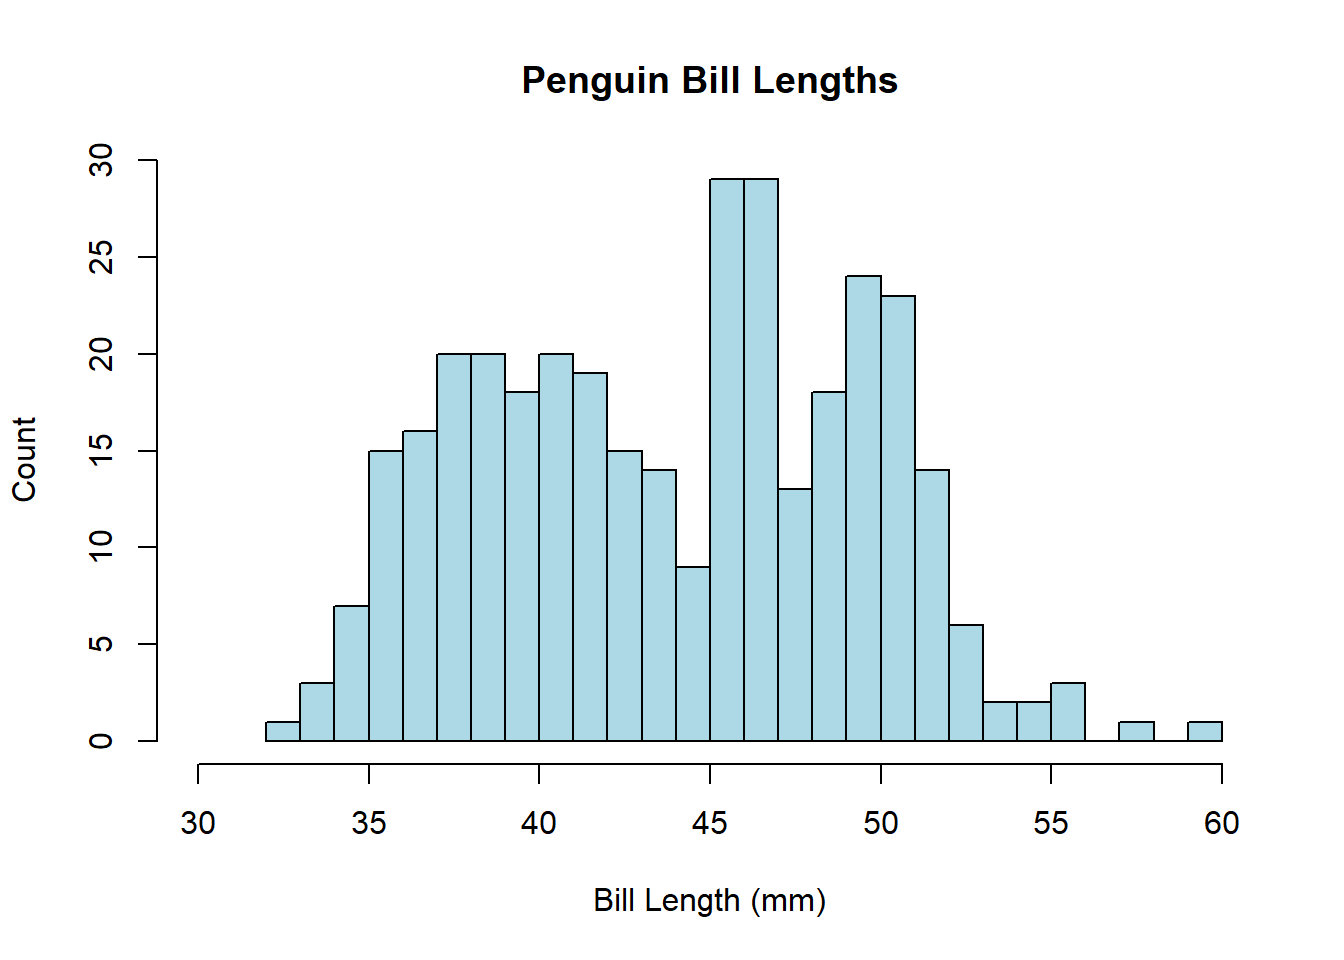
\includegraphics{_main_files/figure-latex/unnamed-chunk-270-3.pdf}

The \textbf{ggplot2} method for generating histograms follows the standard \textbf{ggplot2} syntax: Initialize a plot with \texttt{ggplot()}, and then add layers thereto, specifying aesthetic properties along the way. Here, the layer to add is \texttt{geom\_histogram()}.

\begin{Shaded}
\begin{Highlighting}[]
\SpecialCharTok{\textgreater{}} \FunctionTok{ggplot}\NormalTok{(penguins, }\FunctionTok{aes}\NormalTok{(}\AttributeTok{x =}\NormalTok{ bill\_length\_mm)) }\SpecialCharTok{+}
\SpecialCharTok{+}   \FunctionTok{geom\_histogram}\NormalTok{(}\AttributeTok{fill =} \StringTok{\textquotesingle{}lightblue\textquotesingle{}}\NormalTok{, }\AttributeTok{color =} \StringTok{\textquotesingle{}black\textquotesingle{}}\NormalTok{, }\AttributeTok{bins =} \DecValTok{25}\NormalTok{) }\SpecialCharTok{+}
\SpecialCharTok{+}   \FunctionTok{xlim}\NormalTok{(}\DecValTok{30}\NormalTok{, }\DecValTok{60}\NormalTok{) }\SpecialCharTok{+} \FunctionTok{labs}\NormalTok{(}\AttributeTok{title =} \StringTok{\textquotesingle{}Penguin Bill Lengths\textquotesingle{}}\NormalTok{, }\AttributeTok{x =} \StringTok{\textquotesingle{}Bill Length (mm)\textquotesingle{}}\NormalTok{, }\AttributeTok{y =} \StringTok{\textquotesingle{}Count\textquotesingle{}}\NormalTok{)}
\end{Highlighting}
\end{Shaded}

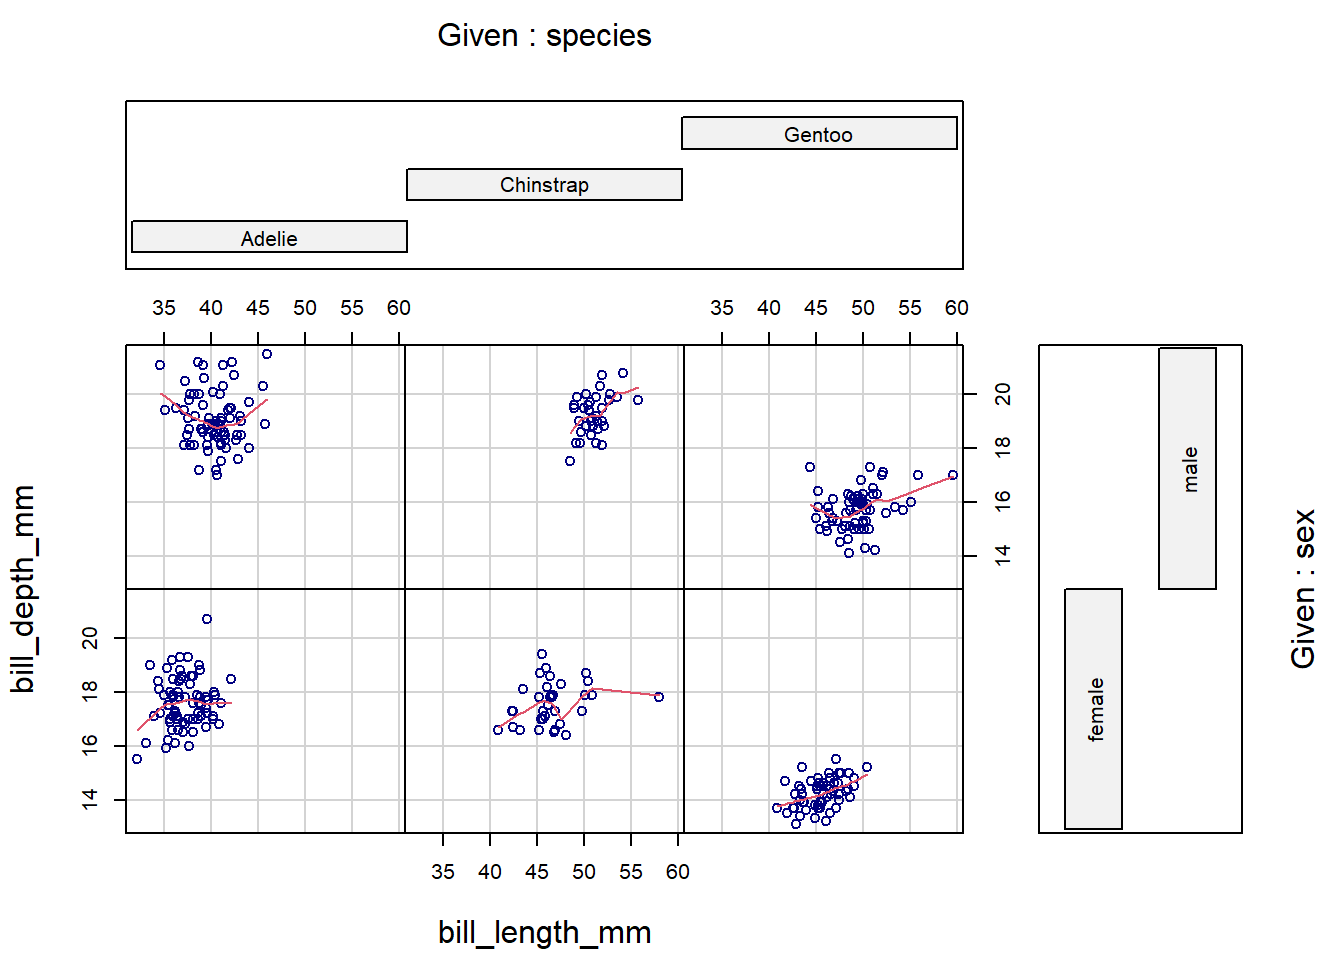
\includegraphics{_main_files/figure-latex/unnamed-chunk-271-1.pdf}

\hypertarget{barplots}{%
\section{Barplots}\label{barplots}}

Visualizing the distribution of categorical data.

\hypertarget{python-42}{%
\subsubsection*{Python}\label{python-42}}
\addcontentsline{toc}{subsubsection}{Python}

For this example, we will generate a bar plot showing how many of each species---Adelie, Chinstrap, Gentoo---we have in our dataset. We go through two ways of doing this here.

First, we use the Matplotlib plotting library to create the bar plot using the function \texttt{bar()}. To start, we determine the number of each species, then use that data to create the bar plot.

\begin{Shaded}
\begin{Highlighting}[]
\OperatorTok{\textgreater{}} \ImportTok{import}\NormalTok{ matplotlib.pyplot }\ImportTok{as}\NormalTok{ plt }
\OperatorTok{+} 
\OperatorTok{+} \CommentTok{\# Determine the number of each species}
\OperatorTok{+}\NormalTok{ adelie\_counts }\OperatorTok{=} \BuiltInTok{len}\NormalTok{(penguins.loc[penguins[}\StringTok{"species"}\NormalTok{]}\OperatorTok{==}\StringTok{"Adelie"}\NormalTok{])}
\OperatorTok{+}\NormalTok{ chinstrap\_counts }\OperatorTok{=} \BuiltInTok{len}\NormalTok{(penguins.loc[penguins[}\StringTok{"species"}\NormalTok{]}\OperatorTok{==}\StringTok{"Chinstrap"}\NormalTok{])}
\OperatorTok{+}\NormalTok{ gentoo\_counts }\OperatorTok{=} \BuiltInTok{len}\NormalTok{(penguins.loc[penguins[}\StringTok{"species"}\NormalTok{]}\OperatorTok{==}\StringTok{"Gentoo"}\NormalTok{])}
\OperatorTok{+} 
\OperatorTok{+} \CommentTok{\# Save the counts information into arrays to be inputted into the bar() function}
\OperatorTok{+}\NormalTok{ spec }\OperatorTok{=}\NormalTok{ [}\StringTok{"Adelie"}\NormalTok{,}\StringTok{"Chinstrap"}\NormalTok{,}\StringTok{"Gentoo"}\NormalTok{]}
\OperatorTok{+}\NormalTok{ counts }\OperatorTok{=}\NormalTok{ [adelie\_counts,chinstrap\_counts,gentoo\_counts]}
\OperatorTok{+} 
\OperatorTok{+}\NormalTok{ plt.clf() }\CommentTok{\# clears the figure to ensure that multiple plots are not overlaid}
\OperatorTok{+}\NormalTok{ plt.bar(spec,counts)}
\OperatorTok{\textless{}}\NormalTok{BarContainer }\BuiltInTok{object}\NormalTok{ of }\DecValTok{3}\NormalTok{ artists}\OperatorTok{\textgreater{}}
\OperatorTok{\textgreater{}}\NormalTok{ plt.show()}
\end{Highlighting}
\end{Shaded}

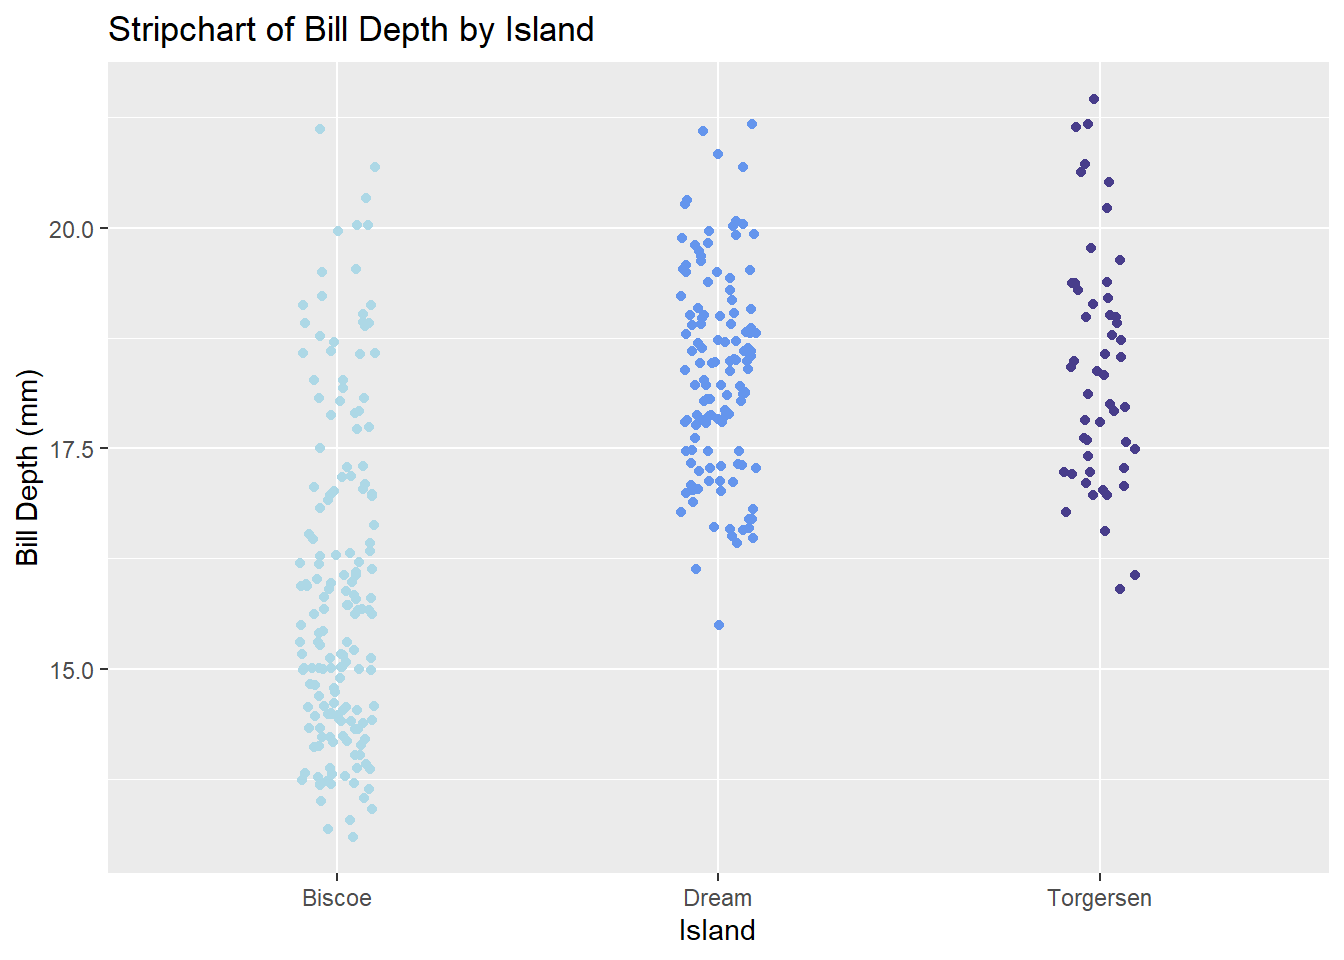
\includegraphics{_main_files/figure-latex/unnamed-chunk-272-1.pdf}

Our data is stored in a \texttt{pandas\ Dataframe}, which has it's own built-in plotting module, \texttt{plot}. Here we create the same bar plot by using the pandas \texttt{bar()} function.

\begin{Shaded}
\begin{Highlighting}[]
\OperatorTok{\textgreater{}}\NormalTok{ plt.clf()}
\OperatorTok{+}\NormalTok{ penguins[}\StringTok{"species"}\NormalTok{].value\_counts().plot.bar()}
\OperatorTok{+}\NormalTok{ plt.show()}
\end{Highlighting}
\end{Shaded}

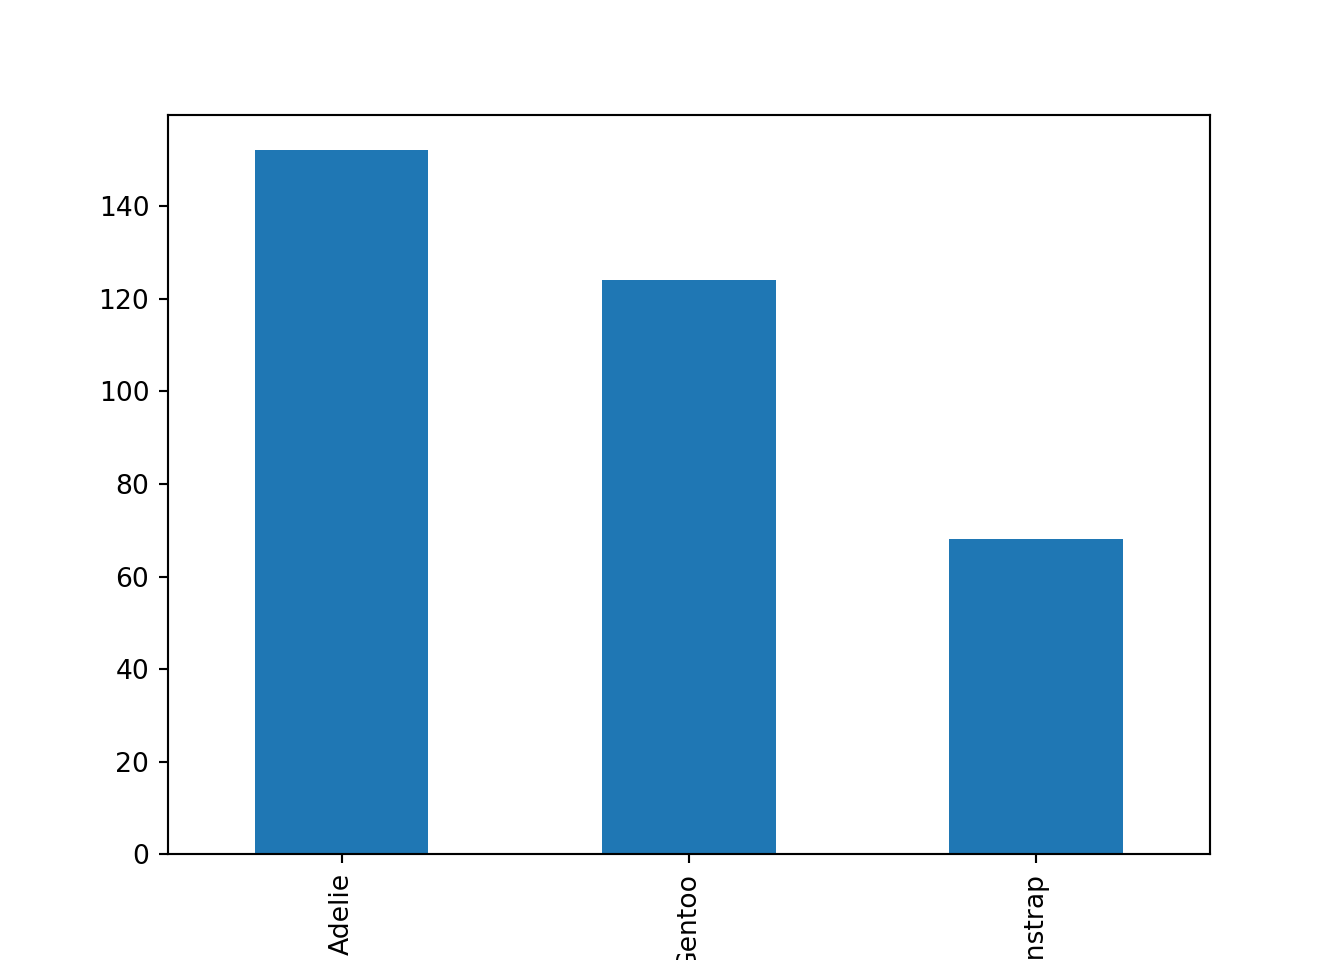
\includegraphics{_main_files/figure-latex/unnamed-chunk-273-3.pdf}
One thing to note here is that we generated the same bar plot containing the same information with way less effort. Using the built-in pandas plotting routine proved to be the more efficient method here.

\hypertarget{r-42}{%
\subsubsection*{R}\label{r-42}}
\addcontentsline{toc}{subsubsection}{R}

To form barplots, we'll first take the \textbf{penguins} data set and create a summary data frame containing the statistics we're looking to plot. Here, that's simply the sample size of each species in the data set.

\begin{Shaded}
\begin{Highlighting}[]
\SpecialCharTok{\textgreater{}}\NormalTok{ species\_counts }\OtherTok{\textless{}{-}} \FunctionTok{as.data.frame}\NormalTok{(}\FunctionTok{xtabs}\NormalTok{(}\SpecialCharTok{\textasciitilde{}}\NormalTok{ species, }\AttributeTok{data =}\NormalTok{ penguins))}
\SpecialCharTok{\textgreater{}}\NormalTok{ species\_counts}
\NormalTok{    species Freq}
\DecValTok{1}\NormalTok{    Adelie  }\DecValTok{152}
\DecValTok{2}\NormalTok{ Chinstrap   }\DecValTok{68}
\DecValTok{3}\NormalTok{    Gentoo  }\DecValTok{124}
\end{Highlighting}
\end{Shaded}

We can plot those values using the \texttt{barplot()} function in base R, specifying arguments along the way to customize the title/axis labeling, bar colors, and range of the y axis. To add values above the bars, we can follow \texttt{barplot()} with a \texttt{text()} call as below.

\begin{Shaded}
\begin{Highlighting}[]
\SpecialCharTok{\textgreater{}}\NormalTok{ penguin\_plot }\OtherTok{\textless{}{-}} \FunctionTok{barplot}\NormalTok{(Freq }\SpecialCharTok{\textasciitilde{}}\NormalTok{ species, }\AttributeTok{data =}\NormalTok{ species\_counts, }\AttributeTok{col =} \FunctionTok{c}\NormalTok{(}\StringTok{\textquotesingle{}lightblue\textquotesingle{}}\NormalTok{, }\StringTok{\textquotesingle{}cornflowerblue\textquotesingle{}}\NormalTok{, }\StringTok{\textquotesingle{}darkslateblue\textquotesingle{}}\NormalTok{),}
\SpecialCharTok{+}                         \AttributeTok{main =} \StringTok{\textquotesingle{}Species Sample Size\textquotesingle{}}\NormalTok{, }
\SpecialCharTok{+}                         \AttributeTok{xlab =} \StringTok{\textquotesingle{}Species\textquotesingle{}}\NormalTok{, }\AttributeTok{ylab =} \StringTok{\textquotesingle{}Count\textquotesingle{}}\NormalTok{, }\AttributeTok{ylim =} \FunctionTok{c}\NormalTok{(}\DecValTok{0}\NormalTok{, }\DecValTok{200}\NormalTok{))}
\SpecialCharTok{\textgreater{}} \FunctionTok{text}\NormalTok{(}\AttributeTok{x =}\NormalTok{ penguin\_plot, }\AttributeTok{y =}\NormalTok{ species\_counts}\SpecialCharTok{$}\NormalTok{Freq }\SpecialCharTok{+} \DecValTok{10}\NormalTok{, }
\SpecialCharTok{+}      \AttributeTok{labels =}\NormalTok{ species\_counts}\SpecialCharTok{$}\NormalTok{Freq)}
\end{Highlighting}
\end{Shaded}

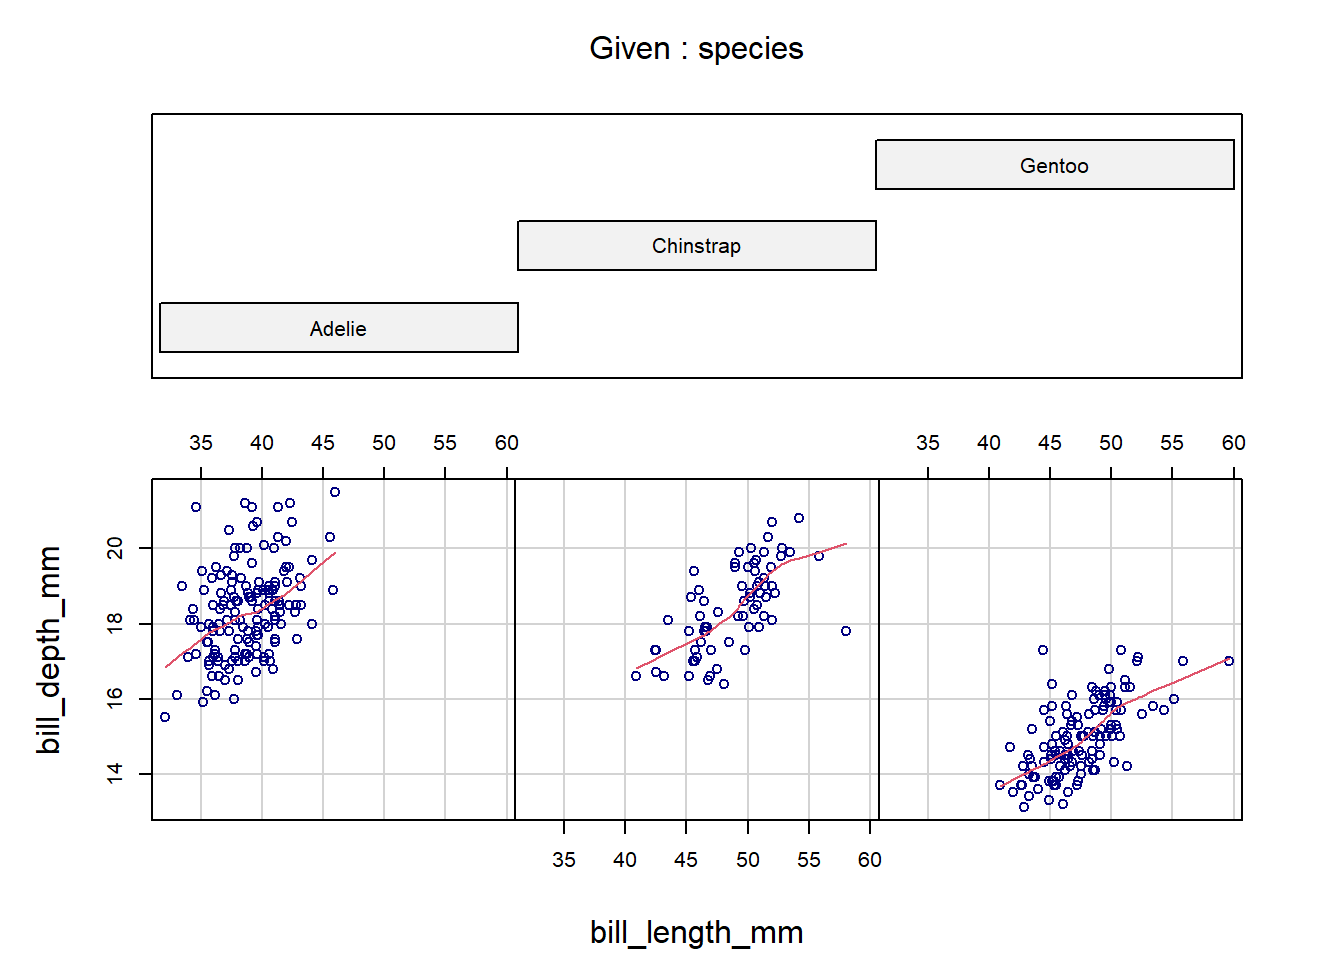
\includegraphics{_main_files/figure-latex/unnamed-chunk-275-1.pdf}

To recreate the barplot above with \textbf{ggplot2}, one can add a \texttt{geom\_bar()} layer to a plot initialized with \texttt{ggplot()}.

\begin{Shaded}
\begin{Highlighting}[]
\SpecialCharTok{\textgreater{}} \FunctionTok{ggplot}\NormalTok{(species\_counts, }\FunctionTok{aes}\NormalTok{(}\AttributeTok{x =}\NormalTok{ species, }\AttributeTok{y =}\NormalTok{ Freq)) }\SpecialCharTok{+}
\SpecialCharTok{+}   \FunctionTok{geom\_bar}\NormalTok{(}\FunctionTok{aes}\NormalTok{(}\AttributeTok{fill =}\NormalTok{ species), }\AttributeTok{stat =} \StringTok{\textquotesingle{}identity\textquotesingle{}}\NormalTok{) }\SpecialCharTok{+}
\SpecialCharTok{+}   \FunctionTok{scale\_fill\_manual}\NormalTok{(}\AttributeTok{values =} \FunctionTok{c}\NormalTok{(}\StringTok{\textquotesingle{}lightblue\textquotesingle{}}\NormalTok{, }\StringTok{\textquotesingle{}cornflowerblue\textquotesingle{}}\NormalTok{, }\StringTok{\textquotesingle{}darkslateblue\textquotesingle{}}\NormalTok{)) }\SpecialCharTok{+} \CommentTok{\# scale\_fill\_manual() is used here for bar{-}color customization}
\SpecialCharTok{+}   \FunctionTok{labs}\NormalTok{(}\AttributeTok{title =} \StringTok{\textquotesingle{}Species Sample Size\textquotesingle{}}\NormalTok{, }\AttributeTok{x =} \StringTok{\textquotesingle{}Species\textquotesingle{}}\NormalTok{, }\AttributeTok{y =} \StringTok{\textquotesingle{}Count\textquotesingle{}}\NormalTok{) }\SpecialCharTok{+}
\SpecialCharTok{+}   \FunctionTok{theme}\NormalTok{(}\AttributeTok{legend.position =} \StringTok{\textquotesingle{}none\textquotesingle{}}\NormalTok{) }\SpecialCharTok{+} \FunctionTok{ylim}\NormalTok{(}\DecValTok{0}\NormalTok{, }\DecValTok{200}\NormalTok{) }\SpecialCharTok{+} \CommentTok{\# For simplicity, we omit the legend here using the code at left}
\SpecialCharTok{+}   \FunctionTok{geom\_text}\NormalTok{(}\FunctionTok{aes}\NormalTok{(}\AttributeTok{label =}\NormalTok{ Freq, }\AttributeTok{vjust =} \SpecialCharTok{{-}}\FloatTok{0.5}\NormalTok{)) }\CommentTok{\# geom\_text() is used here to add counts above the bars}
\end{Highlighting}
\end{Shaded}

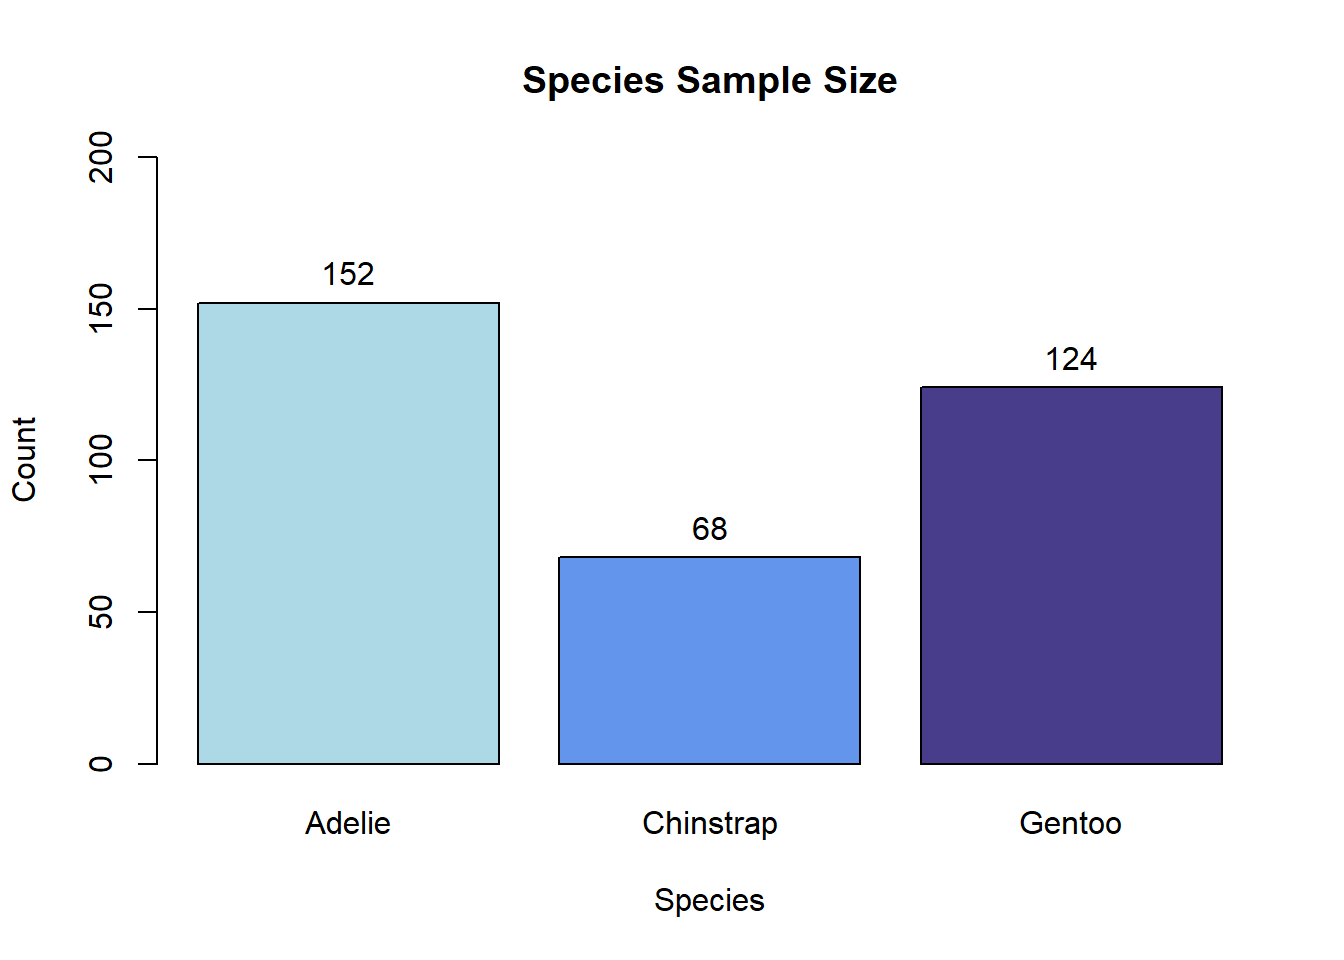
\includegraphics{_main_files/figure-latex/unnamed-chunk-276-1.pdf}

\hypertarget{scatterplot}{%
\section{Scatterplot}\label{scatterplot}}

Visualizing the relationship between two numeric variables.

\hypertarget{python-43}{%
\subsubsection*{Python}\label{python-43}}
\addcontentsline{toc}{subsubsection}{Python}

The \texttt{scatter()} function, part of \textbf{matplotlib}, can produce scatterplots in Python. The \texttt{x} and \texttt{y} arguments specify the points to plot. In the example below, we also use the \texttt{c} and \texttt{marker} arguments to customize the point color and point shape, respectively. The \texttt{xlabel()}, \texttt{ylabel()}, and \texttt{title()} functions customize plot labels.

\begin{Shaded}
\begin{Highlighting}[]
\OperatorTok{\textgreater{}} \ImportTok{import}\NormalTok{ matplotlib.pyplot }\ImportTok{as}\NormalTok{ plt}
\OperatorTok{+} 
\OperatorTok{+}\NormalTok{ penguins\_no\_na }\OperatorTok{=}\NormalTok{ penguins.dropna() }\CommentTok{\# remove NA rows, as we only want to plot present data}
\OperatorTok{+}\NormalTok{ plt.clf() }\CommentTok{\# clear the plotting space to prevent plot overlap}
\OperatorTok{+}\NormalTok{ plt.scatter(x }\OperatorTok{=}\NormalTok{ penguins\_no\_na[}\StringTok{\textquotesingle{}body\_mass\_g\textquotesingle{}}\NormalTok{], y }\OperatorTok{=}\NormalTok{ penguins\_no\_na[}\StringTok{\textquotesingle{}flipper\_length\_mm\textquotesingle{}}\NormalTok{], c }\OperatorTok{=} \StringTok{\textquotesingle{}lightblue\textquotesingle{}}\NormalTok{, marker }\OperatorTok{=} \StringTok{\textquotesingle{}d\textquotesingle{}}\NormalTok{) }\CommentTok{\# \textquotesingle{}d\textquotesingle{} generates diamond markers; learn more about available marker shapes here: https://matplotlib.org/stable/api/markers\_api.html\#module{-}matplotlib.markers}
\OperatorTok{+}\NormalTok{ plt.xlabel(}\StringTok{\textquotesingle{}Body Mass (g)\textquotesingle{}}\NormalTok{)}
\OperatorTok{+}\NormalTok{ plt.ylabel(}\StringTok{\textquotesingle{}Flipper Length (mm)\textquotesingle{}}\NormalTok{)}
\OperatorTok{+}\NormalTok{ plt.title(}\StringTok{\textquotesingle{}Scatterplot of Body Mass and Flipper Length\textquotesingle{}}\NormalTok{)}
\OperatorTok{+} 
\OperatorTok{+}\NormalTok{ plt.show()}
\end{Highlighting}
\end{Shaded}

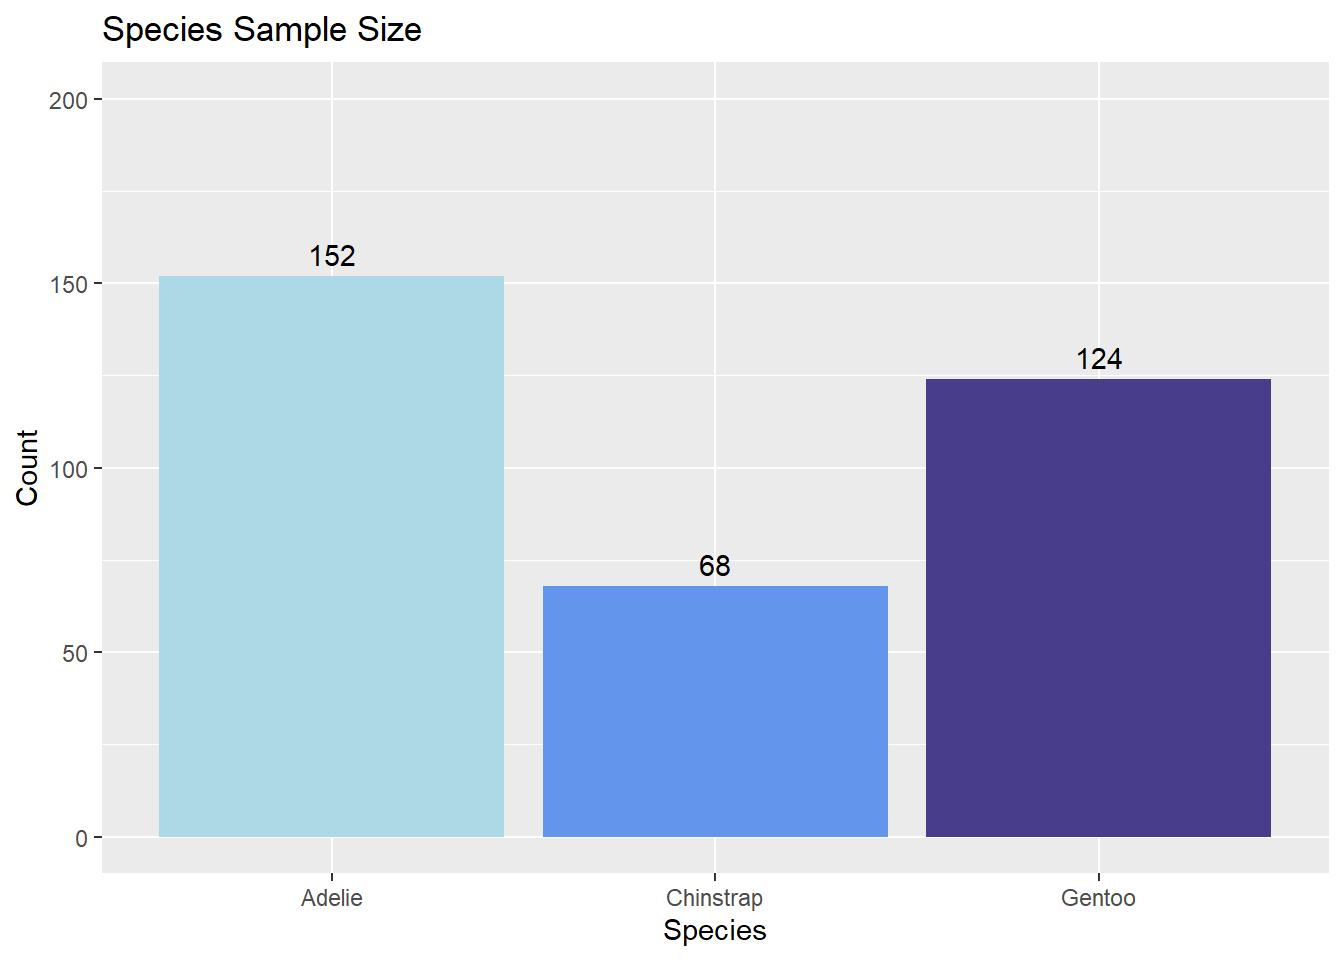
\includegraphics{_main_files/figure-latex/unnamed-chunk-277-1.pdf}

\hypertarget{r-43}{%
\subsubsection*{R}\label{r-43}}
\addcontentsline{toc}{subsubsection}{R}

Scatterplots can be generated in base R with the \texttt{plot()} function. The \texttt{pch} argument below modifies the point shape (e.g., 20 = solid circle; 24 = unfilled triangle; etc.)

\begin{Shaded}
\begin{Highlighting}[]
\SpecialCharTok{\textgreater{}} \FunctionTok{plot}\NormalTok{(}\AttributeTok{x =}\NormalTok{ penguins}\SpecialCharTok{$}\NormalTok{body\_mass\_g, }\AttributeTok{y =}\NormalTok{ penguins}\SpecialCharTok{$}\NormalTok{flipper\_length\_mm, }
\SpecialCharTok{+}      \AttributeTok{col =} \StringTok{\textquotesingle{}navy\textquotesingle{}}\NormalTok{, }\AttributeTok{pch =} \DecValTok{20}\NormalTok{,}
\SpecialCharTok{+}      \AttributeTok{main =} \StringTok{\textquotesingle{}Scatterplot of Body Mass and Flipper Length\textquotesingle{}}\NormalTok{, }
\SpecialCharTok{+}      \AttributeTok{xlab =} \StringTok{\textquotesingle{}Body Mass (g)\textquotesingle{}}\NormalTok{, }\AttributeTok{ylab =} \StringTok{\textquotesingle{}Flipper Length (mm)\textquotesingle{}}\NormalTok{)}
\end{Highlighting}
\end{Shaded}

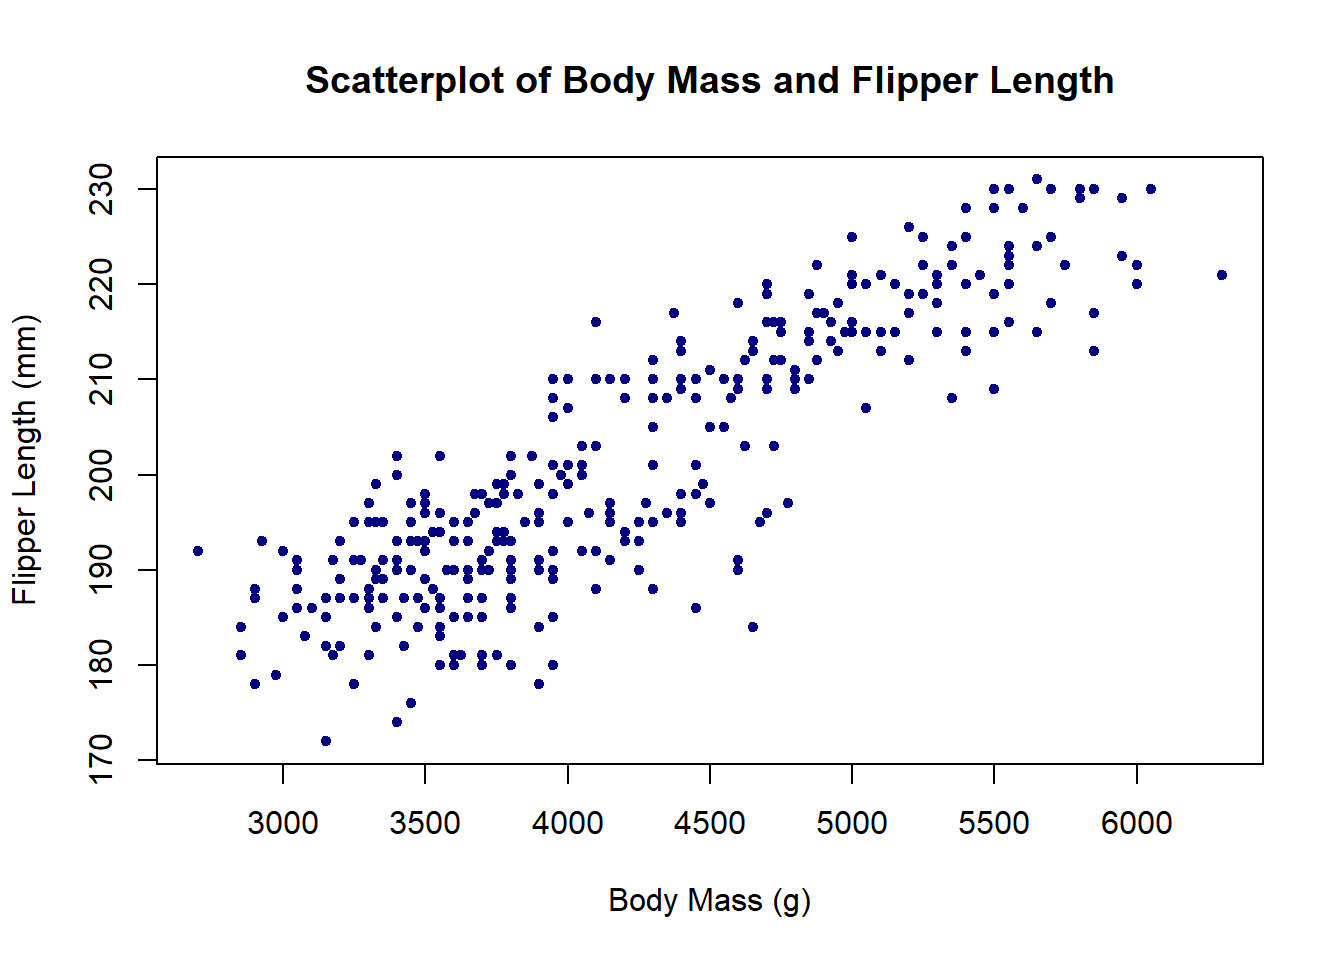
\includegraphics{_main_files/figure-latex/unnamed-chunk-278-3.pdf}

To generate a scatterplot with \textbf{ggplot2}, initialize a plot with \texttt{ggplot()}, then add a layer of points with \texttt{geom\_point()}.

\begin{Shaded}
\begin{Highlighting}[]
\SpecialCharTok{\textgreater{}} \FunctionTok{ggplot}\NormalTok{(penguins, }\FunctionTok{aes}\NormalTok{(}\AttributeTok{x =}\NormalTok{ body\_mass\_g, }\AttributeTok{y =}\NormalTok{ flipper\_length\_mm)) }\SpecialCharTok{+}
\SpecialCharTok{+}   \FunctionTok{geom\_point}\NormalTok{(}\AttributeTok{color =} \StringTok{\textquotesingle{}navy\textquotesingle{}}\NormalTok{) }\SpecialCharTok{+}
\SpecialCharTok{+}   \FunctionTok{labs}\NormalTok{(}\AttributeTok{title =} \StringTok{\textquotesingle{}Scatterplot of Body Mass and Flipper Length\textquotesingle{}}\NormalTok{, }
\SpecialCharTok{+}        \AttributeTok{x =} \StringTok{\textquotesingle{}Body Mass (g)\textquotesingle{}}\NormalTok{, }\AttributeTok{y =} \StringTok{\textquotesingle{}Flipper Length (mm)\textquotesingle{}}\NormalTok{)}
\end{Highlighting}
\end{Shaded}

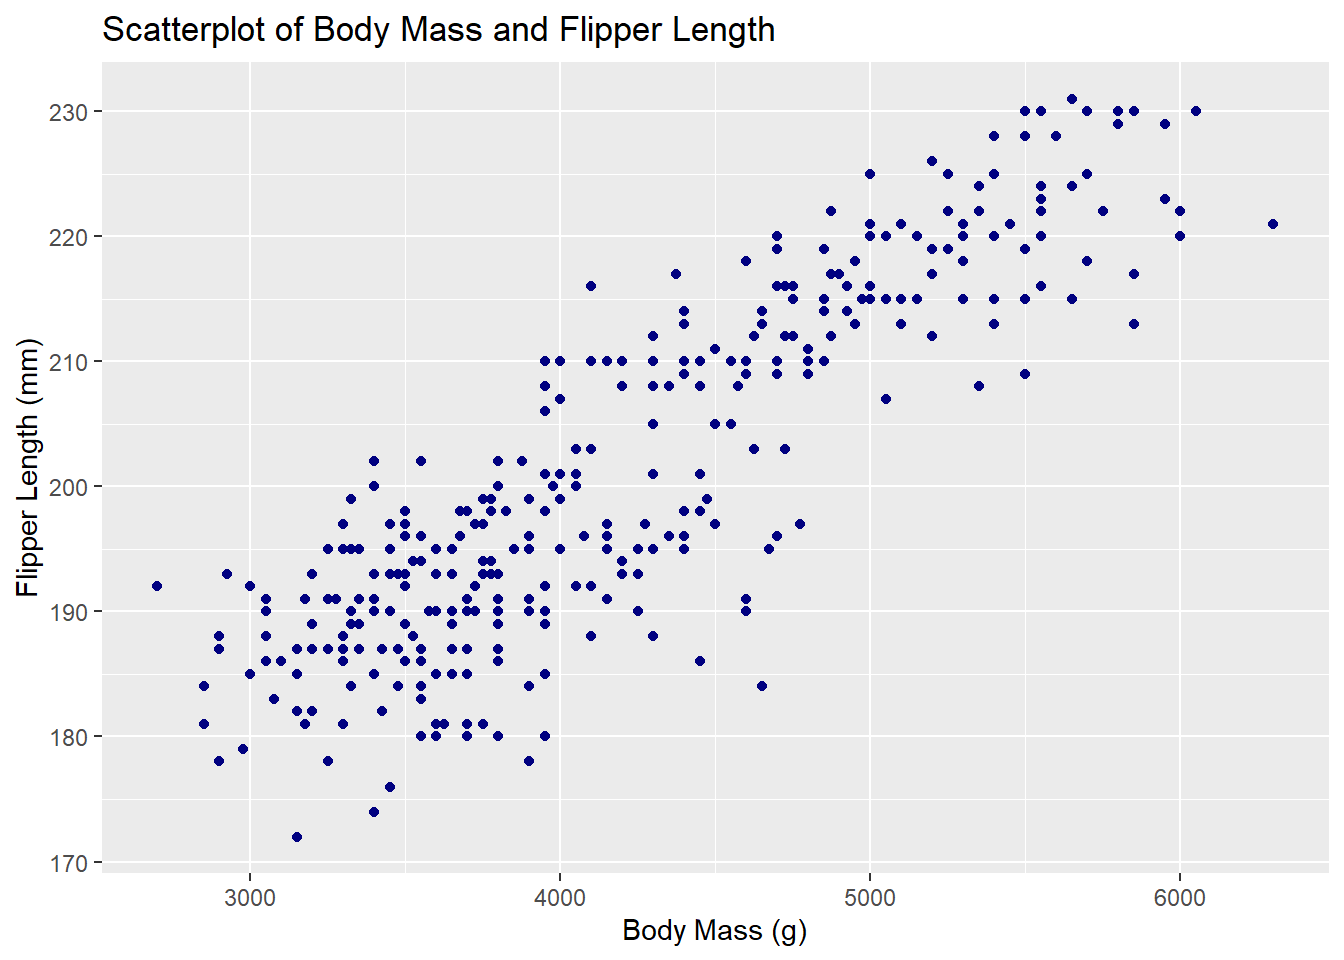
\includegraphics{_main_files/figure-latex/unnamed-chunk-279-1.pdf}

\hypertarget{stripcharts}{%
\section{Stripcharts}\label{stripcharts}}

Stripcharts, or strip plots, are one-dimensional scatterplots. Like boxplots, they reveal the distribution of a numeric variable within levels of a categorical variable.

\hypertarget{python-44}{%
\subsubsection*{Python}\label{python-44}}
\addcontentsline{toc}{subsubsection}{Python}

The \textbf{seaborn} package provides the \texttt{stripplot()} function. Specify which variables you want on the x and y axes. Below we specify island on the y axis to see the distribution of bill\_depth\_mm horizontally. Specify your Pandas data frame using the data argument. Finally create the plot using \texttt{plt.show()} from \textbf{matplotlib}.

\begin{Shaded}
\begin{Highlighting}[]
\OperatorTok{\textgreater{}} \ImportTok{import}\NormalTok{ seaborn }\ImportTok{as}\NormalTok{ sns}
\OperatorTok{+} \ImportTok{import}\NormalTok{ matplotlib.pyplot }\ImportTok{as}\NormalTok{ plt}
\OperatorTok{+}\NormalTok{ sns.stripplot(x}\OperatorTok{=}\StringTok{"bill\_depth\_mm"}\NormalTok{, y}\OperatorTok{=}\StringTok{"island"}\NormalTok{, data}\OperatorTok{=}\NormalTok{penguins)}
\OperatorTok{+}\NormalTok{ plt.show()}
\end{Highlighting}
\end{Shaded}

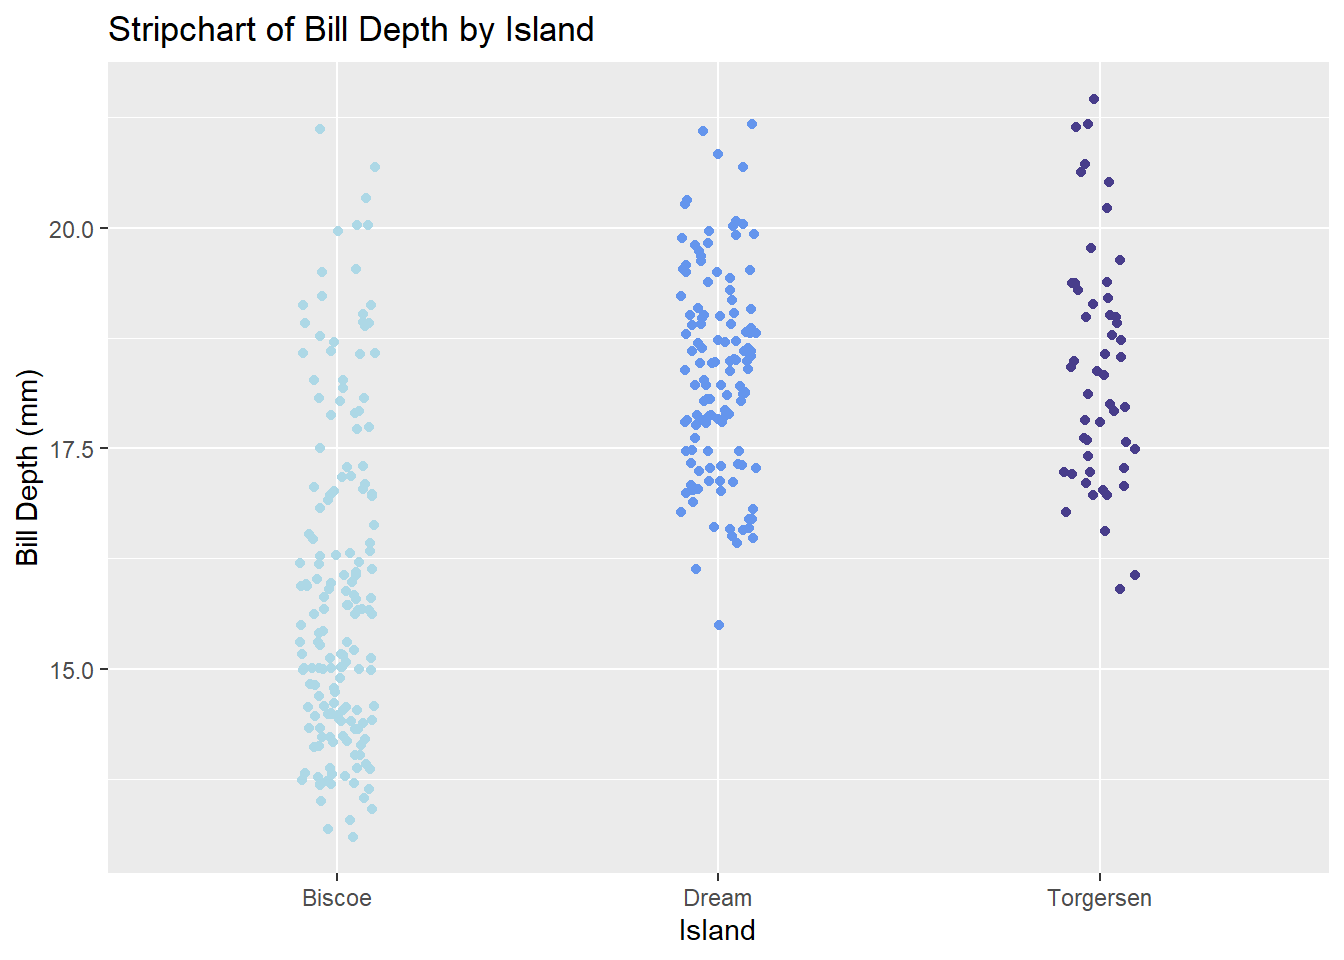
\includegraphics{_main_files/figure-latex/unnamed-chunk-280-1.pdf}

The \href{https://seaborn.pydata.org/generated/seaborn.stripplot.html}{stripplot} help page provides more examples.

\hypertarget{r-44}{%
\subsubsection*{R}\label{r-44}}
\addcontentsline{toc}{subsubsection}{R}

Base R offers the \texttt{stripchart()} function. To indicate the numeric variable and the grouping variable, you can use formula notation: \texttt{numeric\_var\ \textasciitilde{}\ grouping\_var}. Adding \texttt{methhod\ =\ \textquotesingle{}jitter\textquotesingle{}} to the set of arguments spreads the points out slightly within each level of the grouping variable, making it easier to see points that might otherwise be obscured by overlap.

\begin{Shaded}
\begin{Highlighting}[]
\SpecialCharTok{\textgreater{}} \FunctionTok{stripchart}\NormalTok{(bill\_depth\_mm }\SpecialCharTok{\textasciitilde{}}\NormalTok{ island, }\AttributeTok{data =}\NormalTok{ penguins, }
\SpecialCharTok{+}            \AttributeTok{method =} \StringTok{\textquotesingle{}jitter\textquotesingle{}}\NormalTok{,}
\SpecialCharTok{+}            \AttributeTok{ylab =} \StringTok{\textquotesingle{}Island\textquotesingle{}}\NormalTok{, }\AttributeTok{xlab =} \StringTok{\textquotesingle{}Bill Depth (mm)\textquotesingle{}}\NormalTok{, }
\SpecialCharTok{+}            \AttributeTok{main =} \StringTok{\textquotesingle{}Stripchart of Bill Depth by Island\textquotesingle{}}\NormalTok{)}
\end{Highlighting}
\end{Shaded}

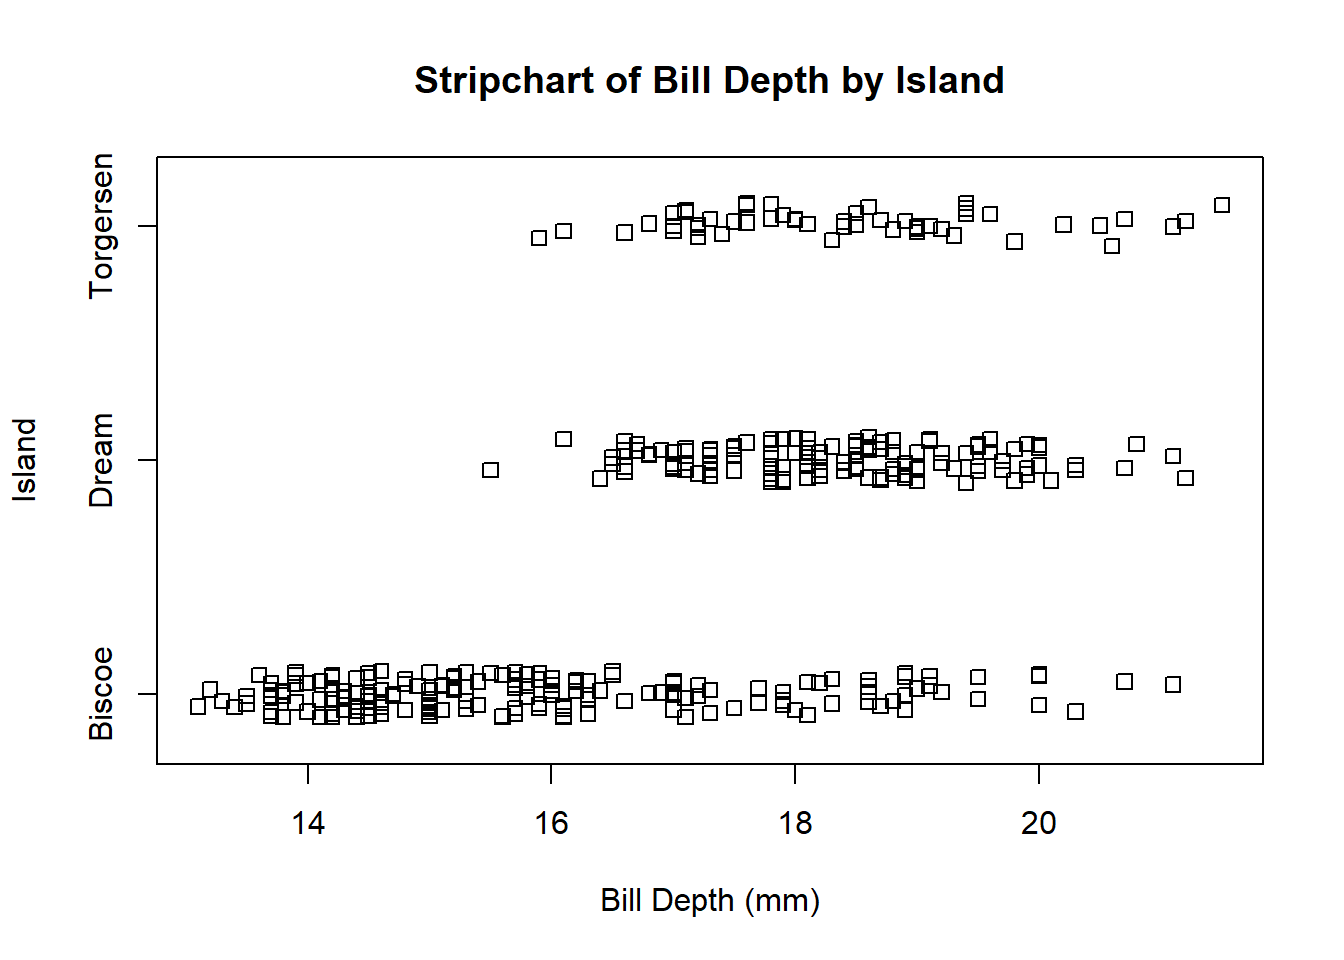
\includegraphics{_main_files/figure-latex/unnamed-chunk-281-3.pdf}

Stripcharts can also be made with \textbf{ggplots2}'s \texttt{geom\_jitter()} function, as shown below. You can control the amount of jitter with a \texttt{position} argument in \texttt{geom\_jitter()}.

\begin{Shaded}
\begin{Highlighting}[]
\SpecialCharTok{\textgreater{}} \FunctionTok{ggplot}\NormalTok{(penguins, }\FunctionTok{aes}\NormalTok{(}\AttributeTok{x =}\NormalTok{ island, }\AttributeTok{y =}\NormalTok{ bill\_depth\_mm)) }\SpecialCharTok{+}
\SpecialCharTok{+}   \FunctionTok{geom\_jitter}\NormalTok{(}\FunctionTok{aes}\NormalTok{(}\AttributeTok{color =}\NormalTok{ island), }\AttributeTok{position =} \FunctionTok{position\_jitter}\NormalTok{(}\FloatTok{0.1}\NormalTok{)) }\SpecialCharTok{+}
\SpecialCharTok{+}   \FunctionTok{scale\_color\_manual}\NormalTok{(}\AttributeTok{values =} \FunctionTok{c}\NormalTok{(}\StringTok{\textquotesingle{}lightblue\textquotesingle{}}\NormalTok{, }\StringTok{\textquotesingle{}cornflowerblue\textquotesingle{}}\NormalTok{, }\StringTok{\textquotesingle{}darkslateblue\textquotesingle{}}\NormalTok{)) }\SpecialCharTok{+} \CommentTok{\# scale\_fill\_manual() is used to manually specify group colors once aes(color = island) is specified in \textasciigrave{}geom\_jitter()\textasciigrave{}}
\SpecialCharTok{+}   \FunctionTok{labs}\NormalTok{(}\AttributeTok{title =} \StringTok{\textquotesingle{}Stripchart of Bill Depth by Island\textquotesingle{}}\NormalTok{, }
\SpecialCharTok{+}        \AttributeTok{x =} \StringTok{\textquotesingle{}Island\textquotesingle{}}\NormalTok{, }\AttributeTok{y =} \StringTok{\textquotesingle{}Bill Depth (mm)\textquotesingle{}}\NormalTok{) }\SpecialCharTok{+}
\SpecialCharTok{+}   \FunctionTok{theme}\NormalTok{(}\AttributeTok{legend.position =} \StringTok{\textquotesingle{}none\textquotesingle{}}\NormalTok{)}
\NormalTok{Warning}\SpecialCharTok{:}\NormalTok{ Removed }\DecValTok{2}\NormalTok{ rows containing missing }\FunctionTok{values}\NormalTok{ (geom\_point).}
\end{Highlighting}
\end{Shaded}

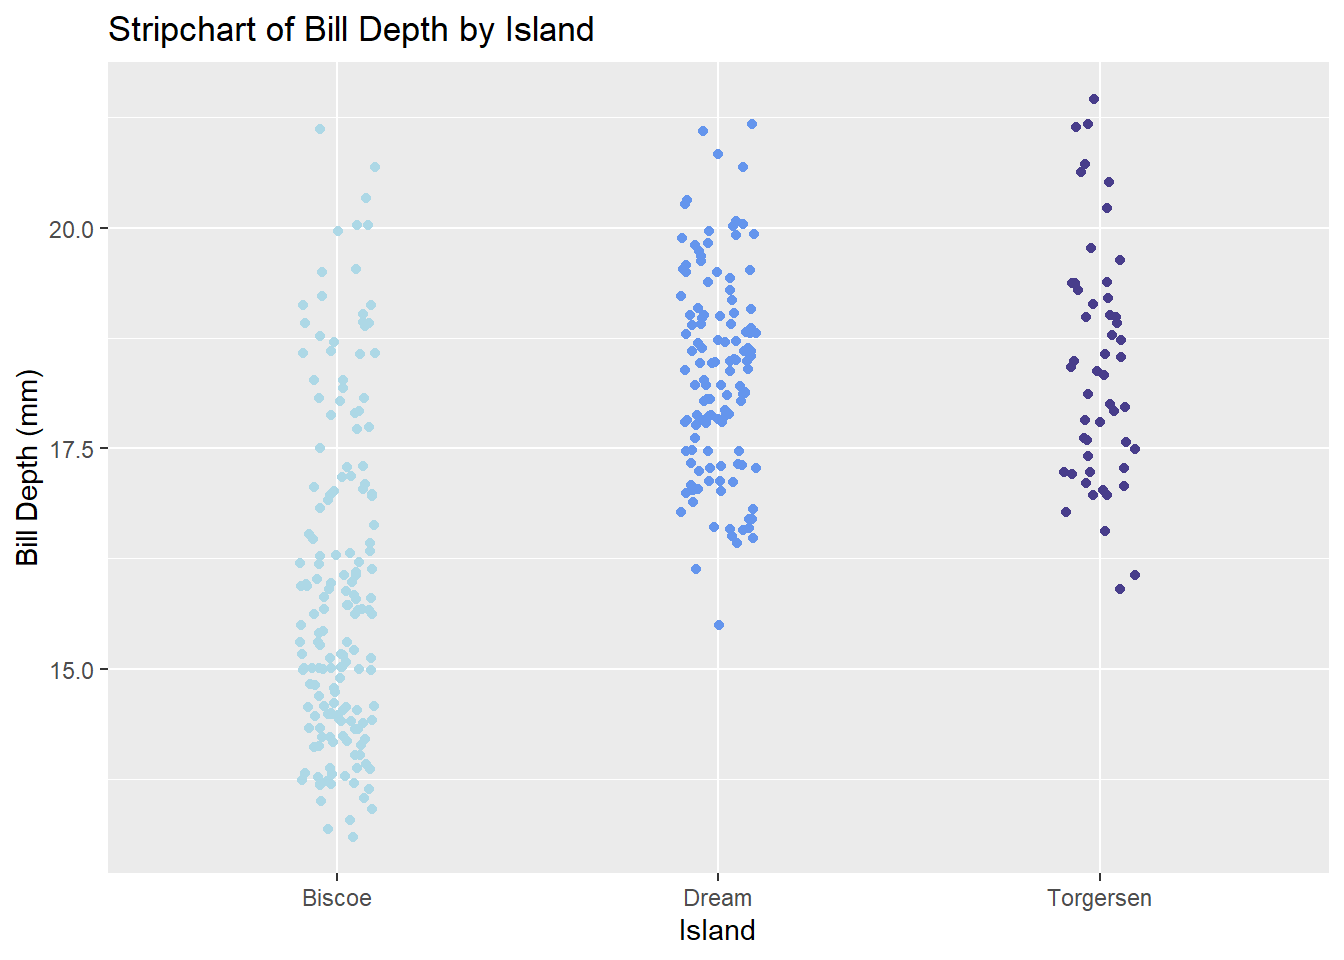
\includegraphics{_main_files/figure-latex/unnamed-chunk-282-1.pdf}

\hypertarget{boxplots}{%
\section{Boxplots}\label{boxplots}}

Visualizing the relationship between a numeric variable and a categorical variable via five-number summaries.

\hypertarget{python-45}{%
\subsubsection*{Python}\label{python-45}}
\addcontentsline{toc}{subsubsection}{Python}

The \texttt{boxplot()} function in seaborn generates boxplots, and matplotlib can be used for the aesthetics of the plot.

\begin{Shaded}
\begin{Highlighting}[]
\OperatorTok{\textgreater{}} \ImportTok{import}\NormalTok{ seaborn }\ImportTok{as}\NormalTok{ sns}
\OperatorTok{+} \ImportTok{import}\NormalTok{ matplotlib.pyplot }\ImportTok{as}\NormalTok{ plt}
\OperatorTok{+}\NormalTok{ plt.figure()}
\OperatorTok{+}\NormalTok{ sns.boxplot(x}\OperatorTok{=}\StringTok{"island"}\NormalTok{, y}\OperatorTok{=}\StringTok{"bill\_depth\_mm"}\NormalTok{, data}\OperatorTok{=}\NormalTok{penguins)}
\OperatorTok{+}\NormalTok{ plt.xlabel(}\StringTok{"Island"}\NormalTok{)}
\OperatorTok{+}\NormalTok{ plt.ylabel(}\StringTok{"Bill Depth (mm)"}\NormalTok{)}
\OperatorTok{+}\NormalTok{ plt.title(}\StringTok{"Bill Depth by Island"}\NormalTok{)}
\OperatorTok{+}\NormalTok{ plt.show()}
\end{Highlighting}
\end{Shaded}

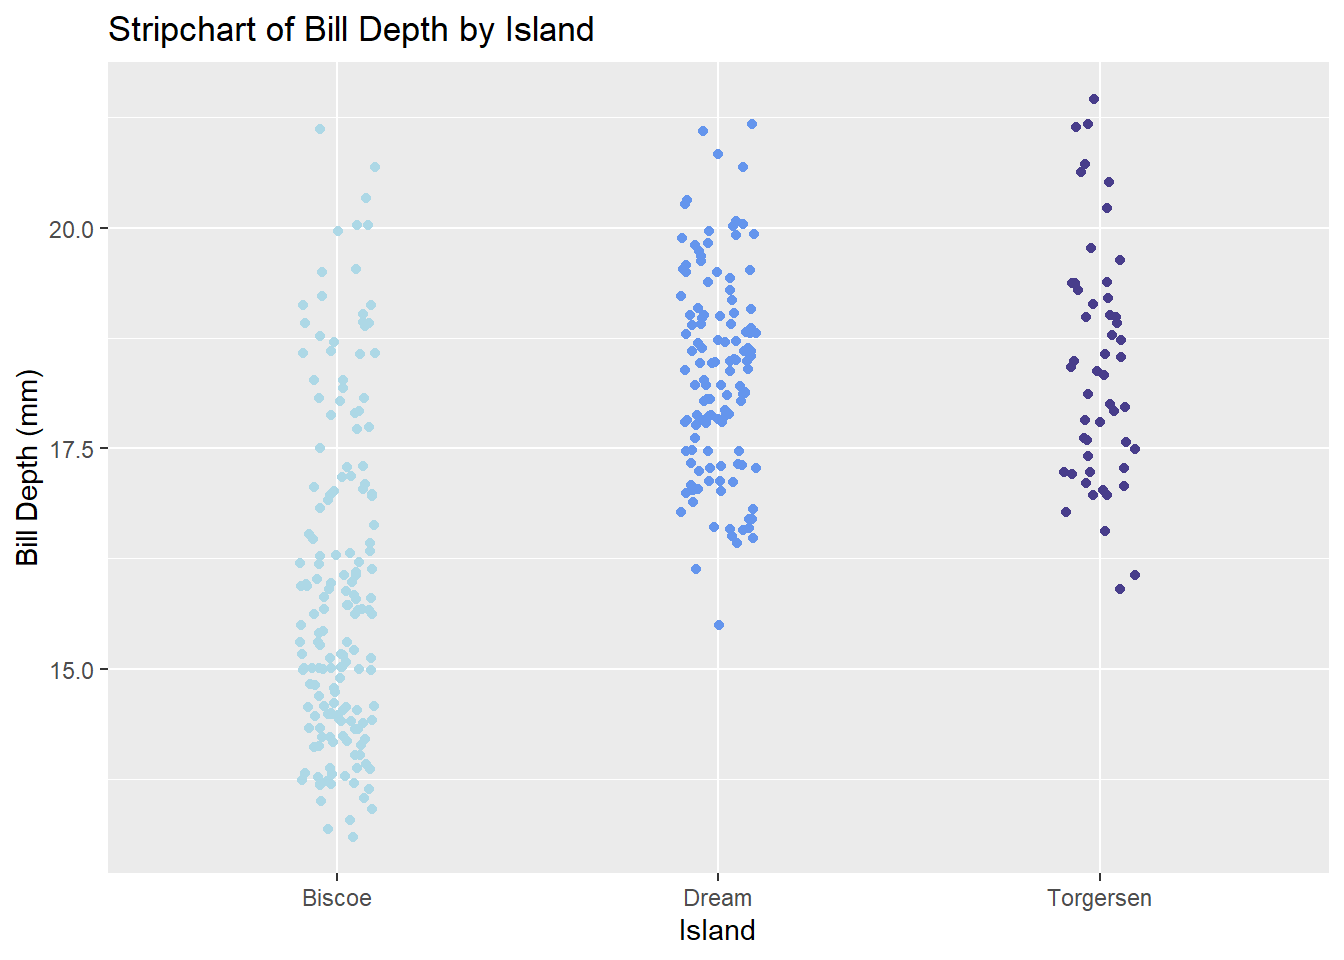
\includegraphics{_main_files/figure-latex/unnamed-chunk-283-1.pdf}

\hypertarget{r-45}{%
\subsubsection*{R}\label{r-45}}
\addcontentsline{toc}{subsubsection}{R}

The \texttt{boxplot()} function in base R generates boxplots, and a user specifies the grouping variable and the numeric variable to be plotted in formula notation: \texttt{y\ \textasciitilde{}\ grouping\_var}.

\begin{Shaded}
\begin{Highlighting}[]
\SpecialCharTok{\textgreater{}} \FunctionTok{boxplot}\NormalTok{(bill\_depth\_mm }\SpecialCharTok{\textasciitilde{}}\NormalTok{ island, }\AttributeTok{data =}\NormalTok{ penguins, }\AttributeTok{col =} \FunctionTok{c}\NormalTok{(}\StringTok{\textquotesingle{}lightblue\textquotesingle{}}\NormalTok{, }\StringTok{\textquotesingle{}cornflowerblue\textquotesingle{}}\NormalTok{, }\StringTok{\textquotesingle{}darkslateblue\textquotesingle{}}\NormalTok{),}
\SpecialCharTok{+}         \AttributeTok{main =} \StringTok{\textquotesingle{}Boxplot of Bill Depth by Island\textquotesingle{}}\NormalTok{, }\AttributeTok{xlab =} \StringTok{\textquotesingle{}Island\textquotesingle{}}\NormalTok{, }\AttributeTok{ylab =} \StringTok{\textquotesingle{}Bill Depth (mm)\textquotesingle{}}\NormalTok{)}
\end{Highlighting}
\end{Shaded}

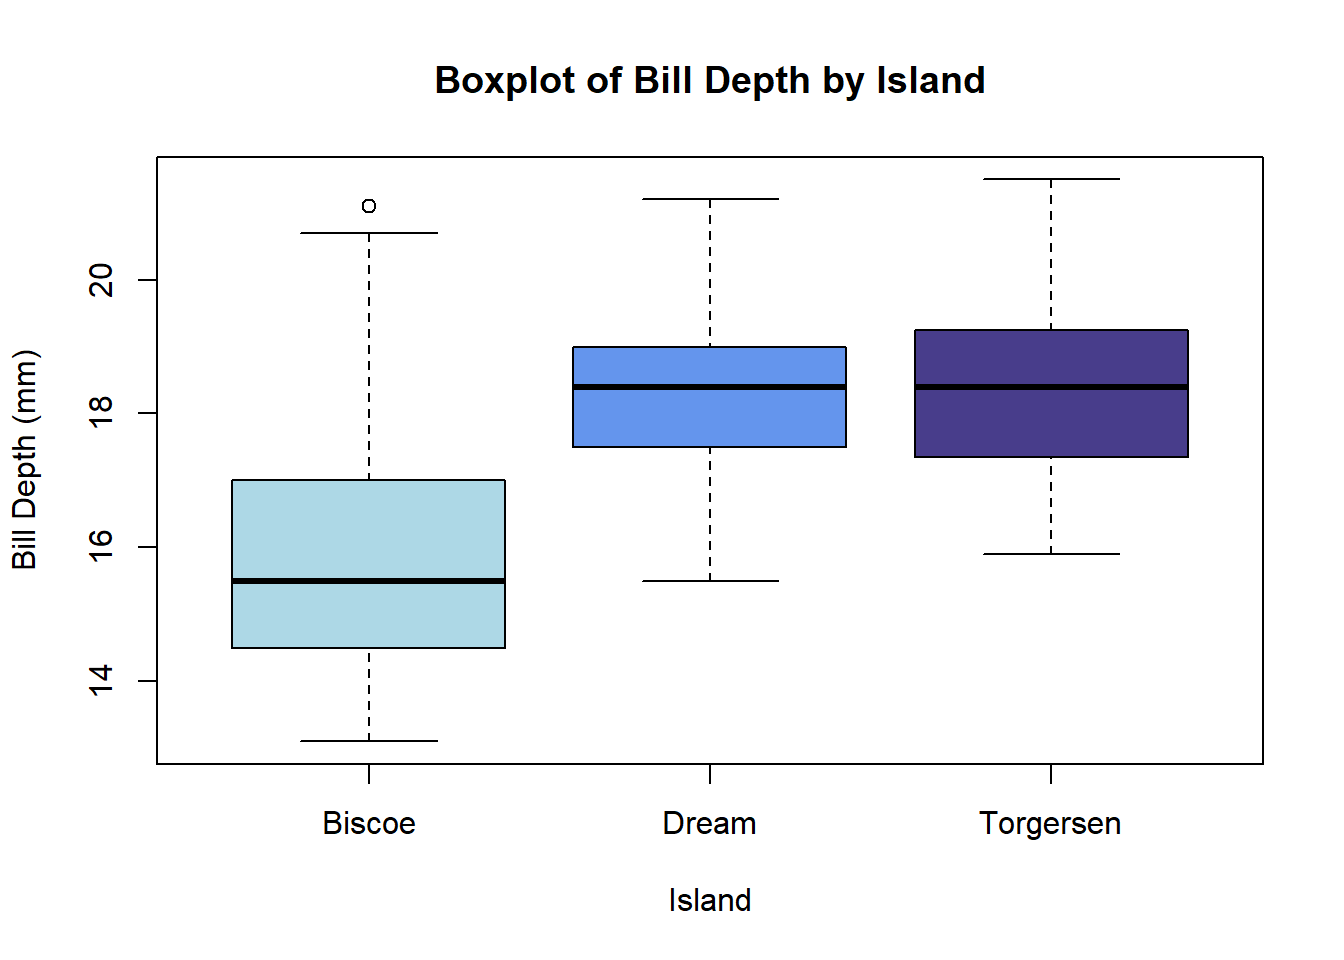
\includegraphics{_main_files/figure-latex/unnamed-chunk-284-3.pdf}

To generate a boxplot with \textbf{ggplot2}, add a \texttt{geom\_boxplot()} layer to a plot initialized with \texttt{ggplot()}.

\begin{Shaded}
\begin{Highlighting}[]
\SpecialCharTok{\textgreater{}} \FunctionTok{ggplot}\NormalTok{(penguins, }\FunctionTok{aes}\NormalTok{(}\AttributeTok{x =}\NormalTok{ island, }\AttributeTok{y =}\NormalTok{ bill\_depth\_mm)) }\SpecialCharTok{+}
\SpecialCharTok{+}   \FunctionTok{geom\_boxplot}\NormalTok{(}\FunctionTok{aes}\NormalTok{(}\AttributeTok{fill =}\NormalTok{ island)) }\SpecialCharTok{+}
\SpecialCharTok{+}   \FunctionTok{scale\_fill\_manual}\NormalTok{(}\AttributeTok{values =} \FunctionTok{c}\NormalTok{(}\StringTok{\textquotesingle{}lightblue\textquotesingle{}}\NormalTok{, }\StringTok{\textquotesingle{}cornflowerblue\textquotesingle{}}\NormalTok{, }\StringTok{\textquotesingle{}darkslateblue\textquotesingle{}}\NormalTok{)) }\SpecialCharTok{+}
\SpecialCharTok{+}   \FunctionTok{labs}\NormalTok{(}\AttributeTok{title =} \StringTok{\textquotesingle{}Boxplot of Bill Depth by Island\textquotesingle{}}\NormalTok{, }
\SpecialCharTok{+}        \AttributeTok{x =} \StringTok{\textquotesingle{}Island\textquotesingle{}}\NormalTok{, }\AttributeTok{y =} \StringTok{\textquotesingle{}Bill Depth (mm)\textquotesingle{}}\NormalTok{) }\SpecialCharTok{+}
\SpecialCharTok{+}   \FunctionTok{theme}\NormalTok{(}\AttributeTok{legend.position =} \StringTok{\textquotesingle{}none\textquotesingle{}}\NormalTok{)}
\end{Highlighting}
\end{Shaded}

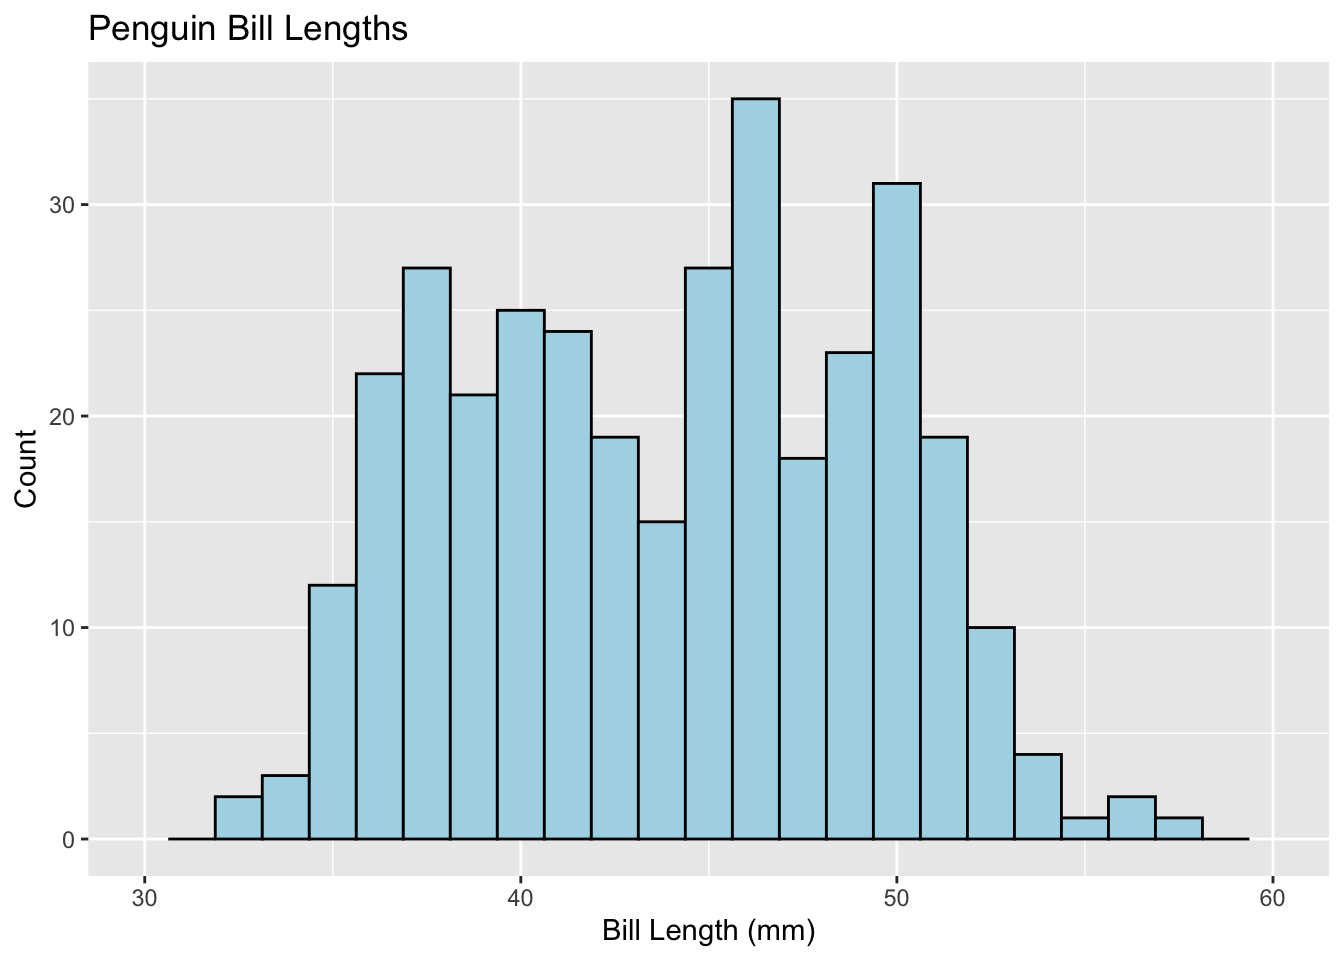
\includegraphics{_main_files/figure-latex/unnamed-chunk-285-1.pdf}

\hypertarget{facet-plots}{%
\section{Facet plots}\label{facet-plots}}

Facet plots (also called trellis plots, lattice plots, and conditional plots) are comprised of multiple smaller plots, where each subplot contains a subset of the overall data, with subsets defined by one or more faceting variables.

\hypertarget{python-46}{%
\subsubsection*{Python}\label{python-46}}
\addcontentsline{toc}{subsubsection}{Python}

The seaborn package provides several functions for creating facet plots, including \texttt{relplot()}, \texttt{displot()}, \texttt{catplot()}, and \texttt{lmplot()}. Below we demonstrate the \texttt{lmplot()} function which allows you to create scatter plots at certain levels of categorical variable. Specify your x and y variables as character strings using the \texttt{x} and \texttt{y} arguments, respectively. Specing the grouping variable using either the \texttt{col} or \texttt{row} arguments. By default a linear-squares lines is added to the plot. Setting \texttt{ci\ =\ None} suppresses the confidence interval ribbon.

\begin{Shaded}
\begin{Highlighting}[]
\OperatorTok{\textgreater{}}\NormalTok{ plt.clf()}
\OperatorTok{+}\NormalTok{ sns.lmplot(x }\OperatorTok{=} \StringTok{"bill\_length\_mm"}\NormalTok{, y }\OperatorTok{=} \StringTok{"bill\_depth\_mm"}\NormalTok{, col }\OperatorTok{=} \StringTok{"species"}\NormalTok{,}
\OperatorTok{+}\NormalTok{           data }\OperatorTok{=}\NormalTok{ penguins, ci }\OperatorTok{=} \VariableTok{None}\NormalTok{)}
\end{Highlighting}
\end{Shaded}

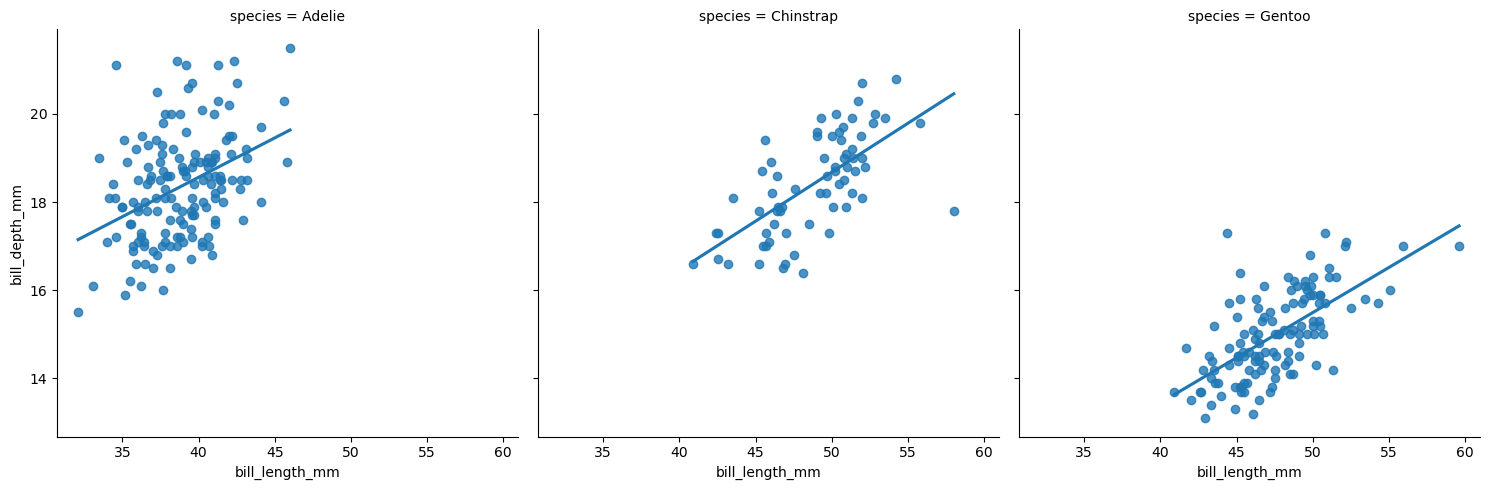
\includegraphics{_main_files/figure-latex/unnamed-chunk-286-1.pdf}

To facet by two variables, provide variables to both the \texttt{col} and \texttt{row} arguments.

\begin{Shaded}
\begin{Highlighting}[]
\OperatorTok{\textgreater{}}\NormalTok{ plt.clf()}
\OperatorTok{+}\NormalTok{ sns.lmplot(x }\OperatorTok{=} \StringTok{"bill\_length\_mm"}\NormalTok{, y }\OperatorTok{=} \StringTok{"bill\_depth\_mm"}\NormalTok{, }
\OperatorTok{+}\NormalTok{            col }\OperatorTok{=} \StringTok{"species"}\NormalTok{, row }\OperatorTok{=} \StringTok{"sex"}\NormalTok{,}
\OperatorTok{+}\NormalTok{            data }\OperatorTok{=}\NormalTok{ penguins, ci }\OperatorTok{=} \VariableTok{None}\NormalTok{)}
\end{Highlighting}
\end{Shaded}

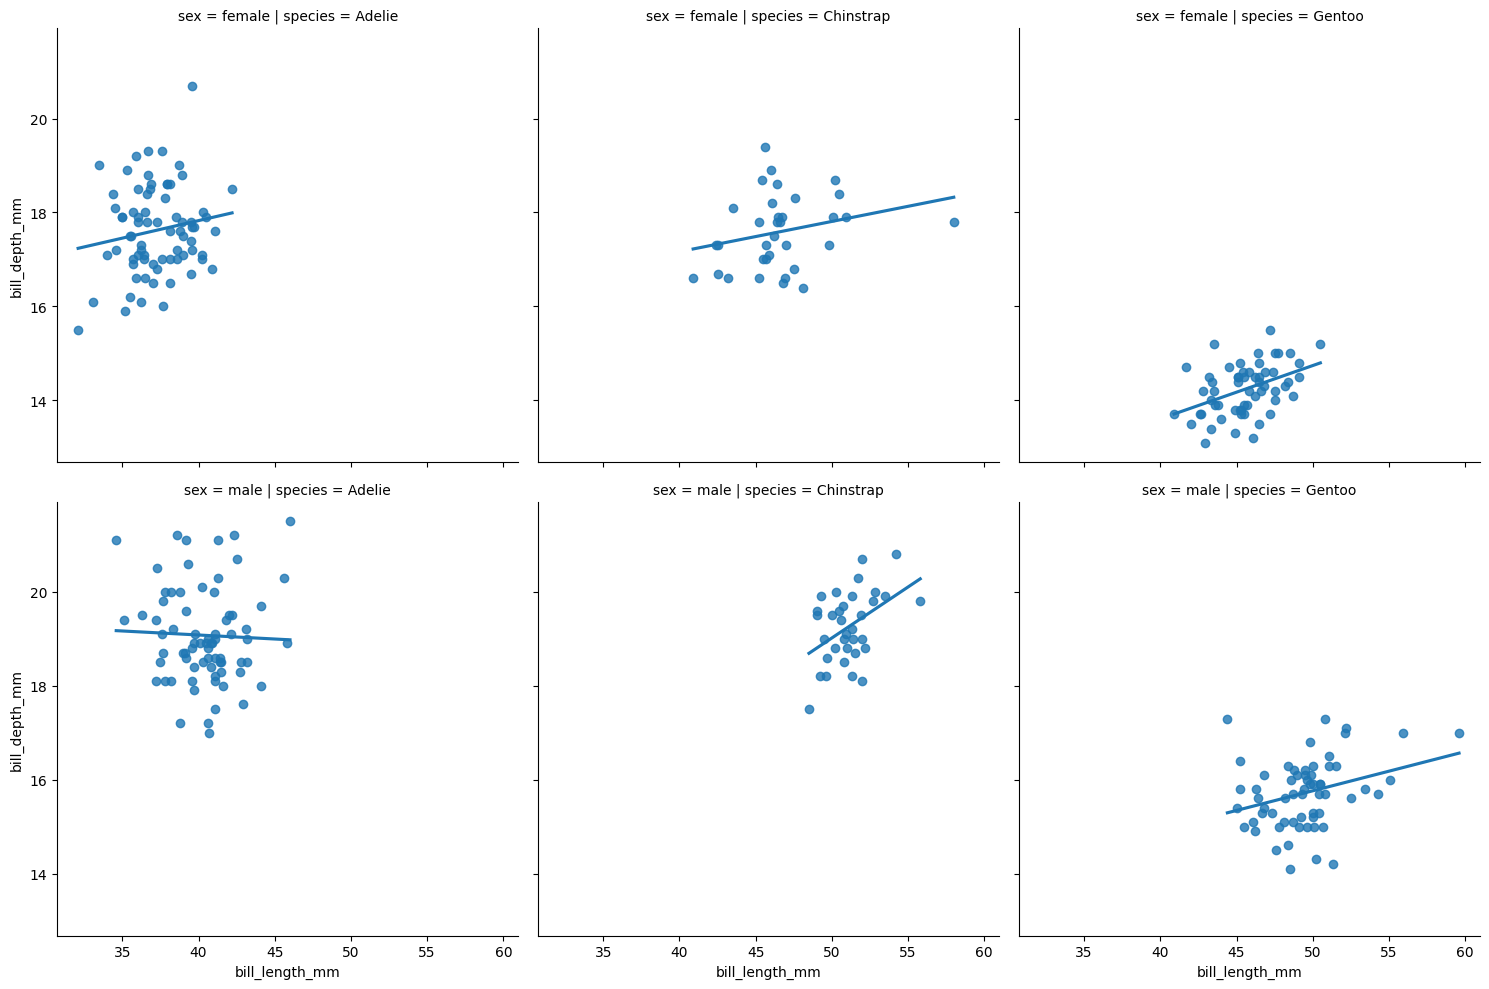
\includegraphics{_main_files/figure-latex/unnamed-chunk-287-3.pdf}

Set \texttt{lowess\ =\ True} for smooth trend lines. Notice also that color can be mapped to the same variable used for faceting.

\begin{Shaded}
\begin{Highlighting}[]
\OperatorTok{\textgreater{}}\NormalTok{ plt.clf()}
\OperatorTok{+}\NormalTok{ sns.lmplot(x }\OperatorTok{=} \StringTok{"bill\_length\_mm"}\NormalTok{, y }\OperatorTok{=} \StringTok{"bill\_depth\_mm"}\NormalTok{, }
\OperatorTok{+}\NormalTok{            col }\OperatorTok{=} \StringTok{"species"}\NormalTok{, hue }\OperatorTok{=} \StringTok{"species"}\NormalTok{,}
\OperatorTok{+}\NormalTok{            data }\OperatorTok{=}\NormalTok{ penguins, ci }\OperatorTok{=} \VariableTok{None}\NormalTok{, lowess }\OperatorTok{=} \VariableTok{True}\NormalTok{)}
\end{Highlighting}
\end{Shaded}

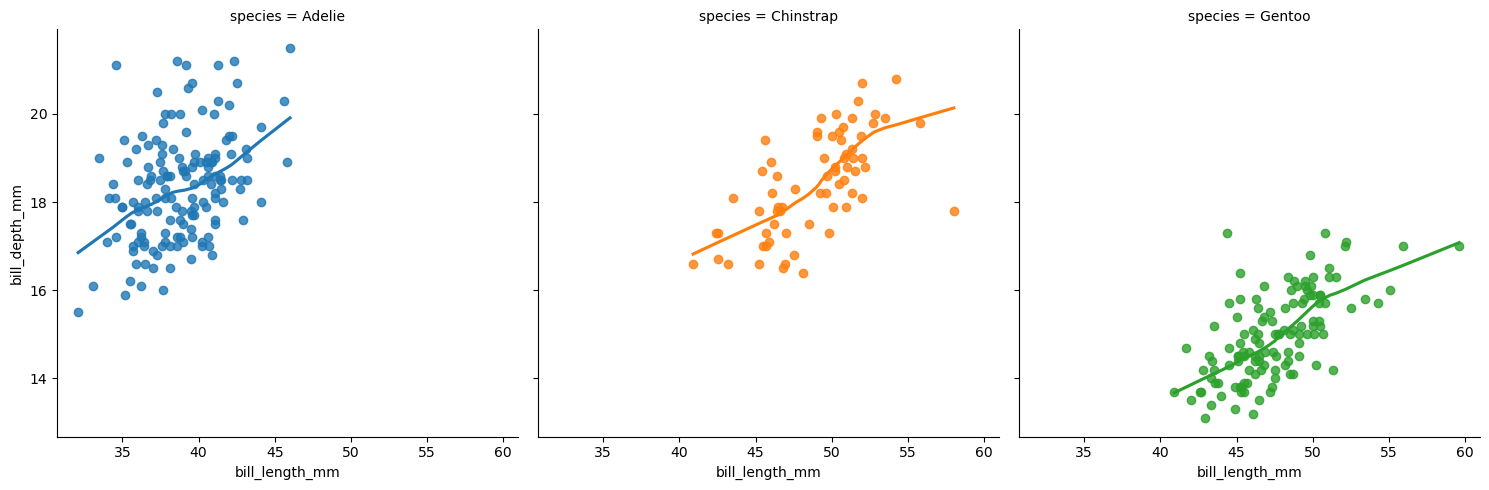
\includegraphics{_main_files/figure-latex/unnamed-chunk-288-5.pdf}

The \href{https://seaborn.pydata.org/generated/seaborn.lmplot.html\#seaborn.lmplot}{lmplot} help page showcases other examples.

\hypertarget{r-46}{%
\subsubsection*{R}\label{r-46}}
\addcontentsline{toc}{subsubsection}{R}

The \texttt{coplot()} function in base R produces conditioning plots using formula notation: \texttt{y\ \textasciitilde{}\ x\ \textbar{}\ grouping\_var}. The \texttt{rows} and \texttt{columns} arguments control layout. Below we specify one row of plots. The \texttt{panel} argument controls what action is carried out in each plot. The default is a scatterplot. Below we use the base R \texttt{panel.smooth} function to create scatter plots with a smooth trend line.

\begin{Shaded}
\begin{Highlighting}[]
\SpecialCharTok{\textgreater{}} \FunctionTok{coplot}\NormalTok{(bill\_depth\_mm }\SpecialCharTok{\textasciitilde{}}\NormalTok{ bill\_length\_mm }\SpecialCharTok{|}\NormalTok{ species, }
\SpecialCharTok{+}        \AttributeTok{data =}\NormalTok{ penguins,}
\SpecialCharTok{+}        \AttributeTok{panel =}\NormalTok{ panel.smooth,}
\SpecialCharTok{+}        \AttributeTok{rows =} \DecValTok{1}\NormalTok{, }\AttributeTok{col =} \StringTok{"navy"}\NormalTok{)}
\end{Highlighting}
\end{Shaded}

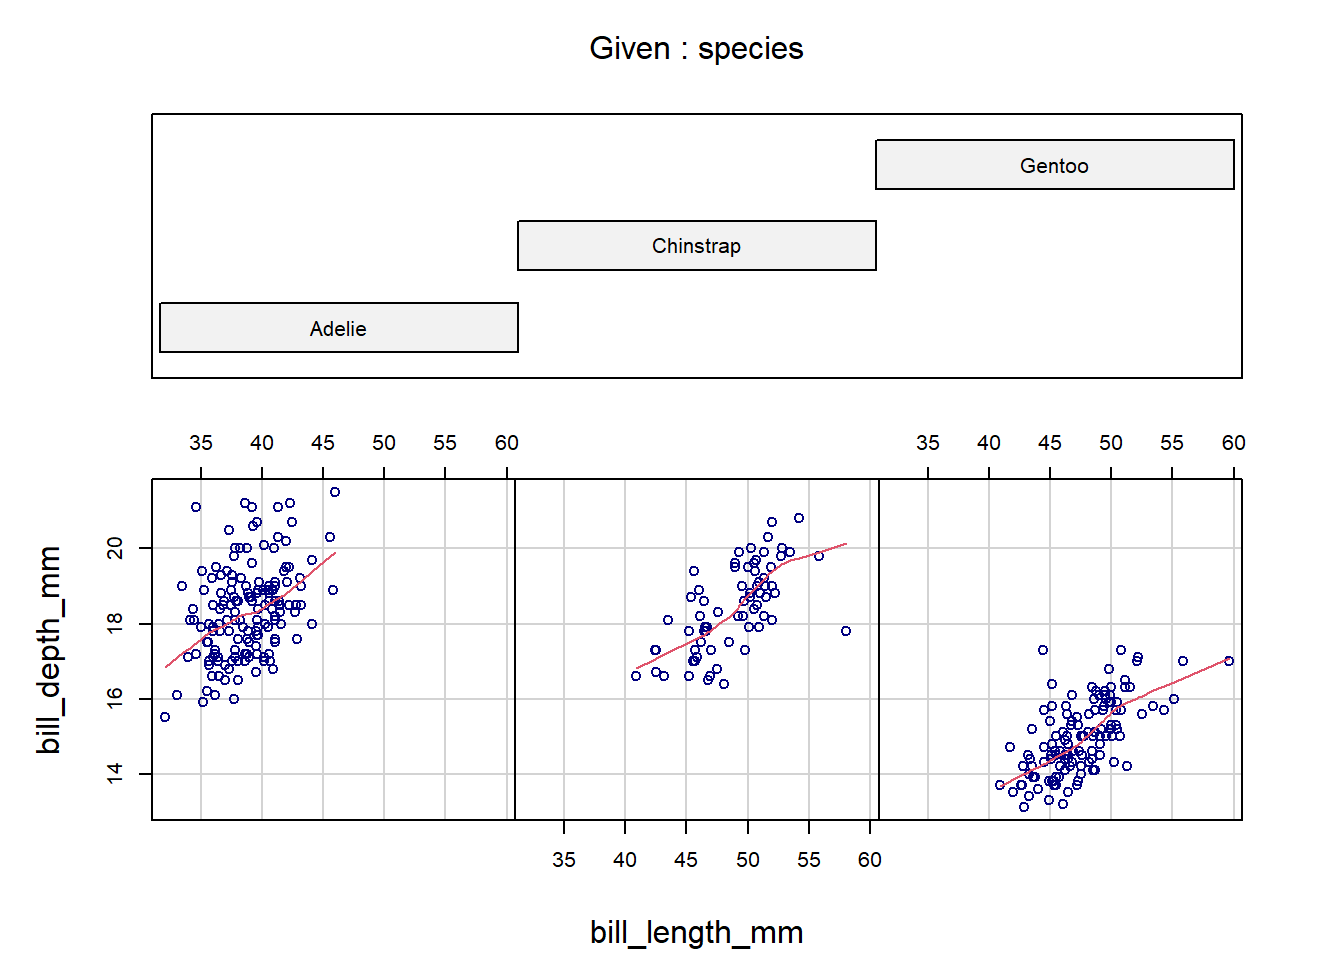
\includegraphics{_main_files/figure-latex/unnamed-chunk-289-7.pdf}

To condition on two variables, use formula notation with syntax: \texttt{y\ \textasciitilde{}\ x\ \textbar{}\ grp\_var1\ *\ grp\_var2}.

\begin{Shaded}
\begin{Highlighting}[]
\SpecialCharTok{\textgreater{}} \FunctionTok{coplot}\NormalTok{(bill\_depth\_mm }\SpecialCharTok{\textasciitilde{}}\NormalTok{ bill\_length\_mm }\SpecialCharTok{|}\NormalTok{ species }\SpecialCharTok{*}\NormalTok{ sex, }
\SpecialCharTok{+}        \AttributeTok{data =}\NormalTok{ penguins,}
\SpecialCharTok{+}        \AttributeTok{panel =}\NormalTok{ panel.smooth,}
\SpecialCharTok{+}        \AttributeTok{col =} \StringTok{"navy"}\NormalTok{)}
\end{Highlighting}
\end{Shaded}

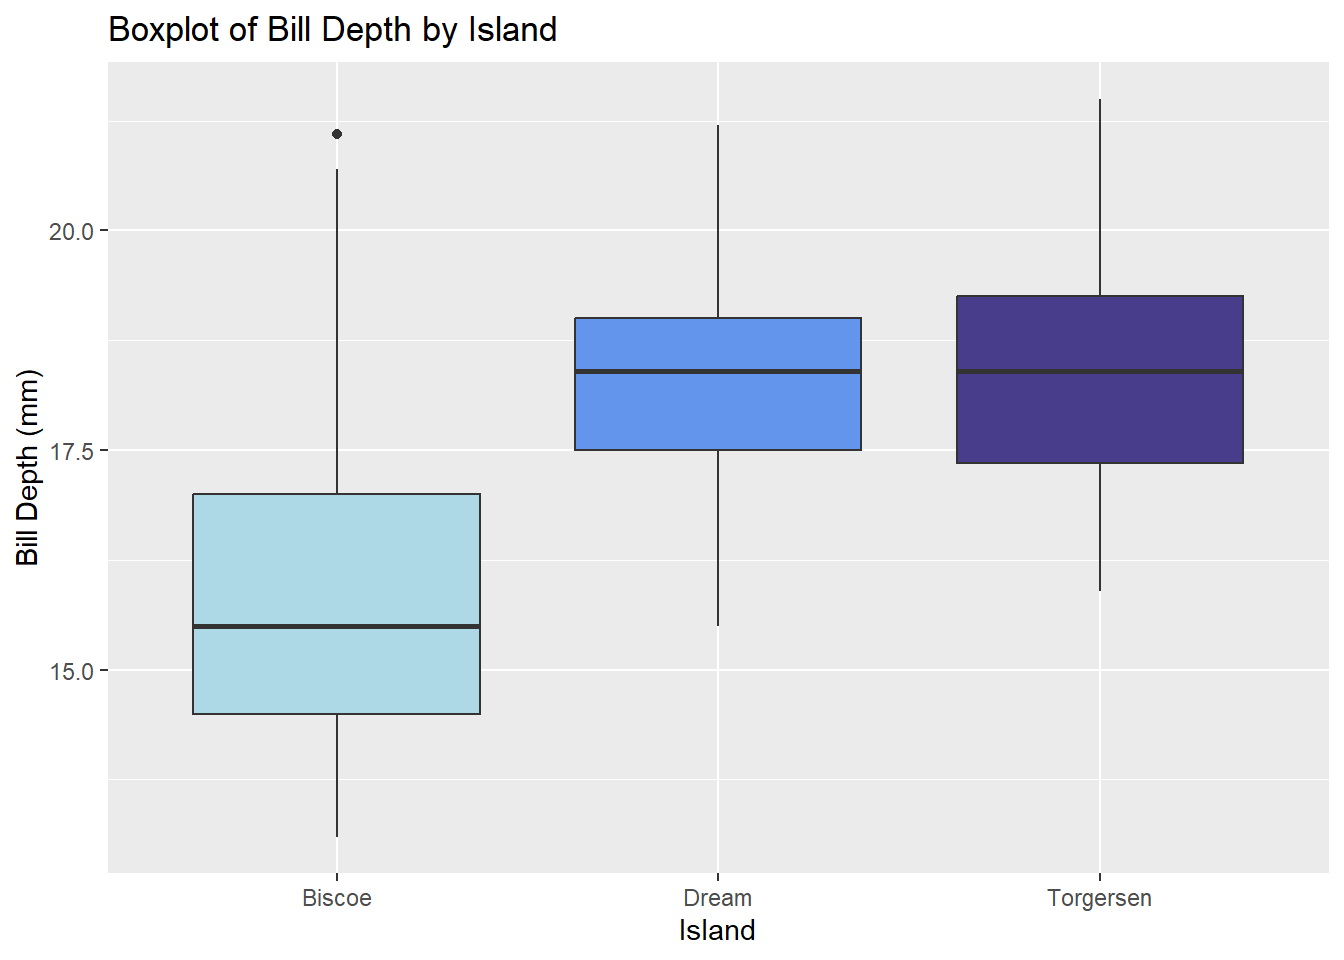
\includegraphics{_main_files/figure-latex/unnamed-chunk-290-1.pdf}

The labels of the conditioning variables unfortunately use a lot of real estate in the margins, and there is no easy way to modify that. However, this design works quite well when we condition on a \emph{numeric variable}. The \texttt{coplot()} function automatically creates overlapping group intervals to condition on, and the stacked layout of the labels helps us visualize how the relationship between y and x changes between the groups. To manually set the number of groups, use the \texttt{number} argument. Below we specify 4 groups to be generated for ``bill\_length\_mm''.

\begin{Shaded}
\begin{Highlighting}[]
\SpecialCharTok{\textgreater{}} \FunctionTok{coplot}\NormalTok{(flipper\_length\_mm }\SpecialCharTok{\textasciitilde{}}\NormalTok{ body\_mass\_g }\SpecialCharTok{|}\NormalTok{ bill\_length\_mm, }
\SpecialCharTok{+}        \AttributeTok{data =}\NormalTok{ penguins,}
\SpecialCharTok{+}        \AttributeTok{panel =}\NormalTok{ panel.smooth,}
\SpecialCharTok{+}        \AttributeTok{number =} \DecValTok{4}\NormalTok{, }
\SpecialCharTok{+}        \AttributeTok{rows =} \DecValTok{1}\NormalTok{, }\AttributeTok{col =} \StringTok{"navy"}\NormalTok{)}
\end{Highlighting}
\end{Shaded}

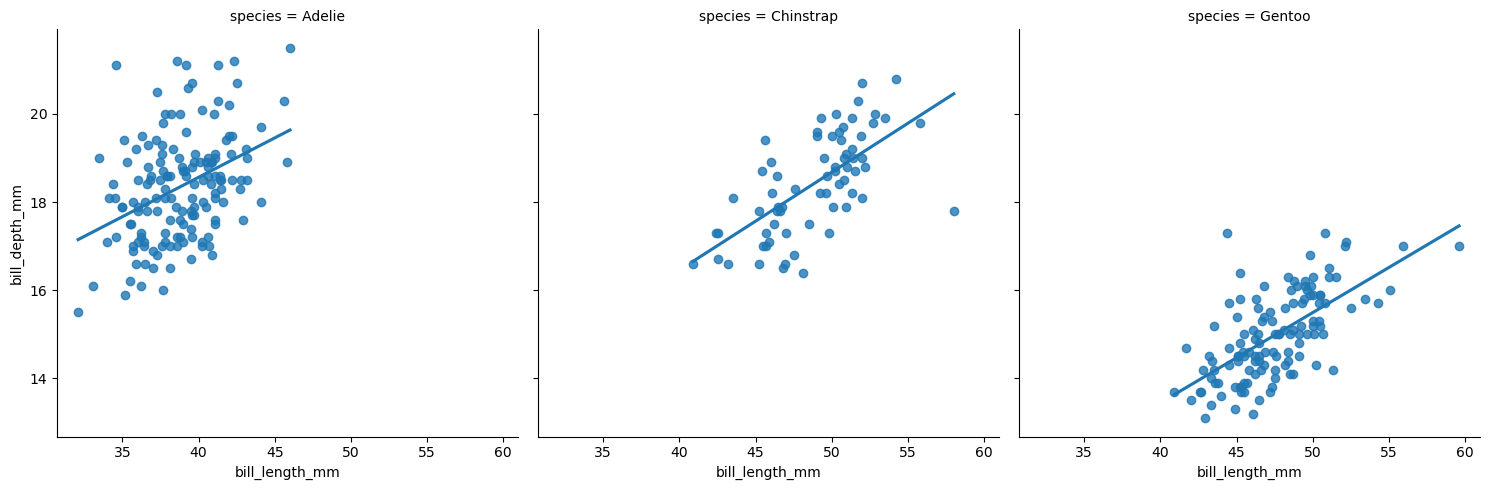
\includegraphics{_main_files/figure-latex/unnamed-chunk-291-1.pdf}

Alternatively, \textbf{ggplot2} provides a intuitive and easy-to-use method for generating facet plots: A user specifies the aesthetics of the plot using standard \textbf{ggplot2} syntax (i.e., as a series of added layers) and then adds an additional call, \texttt{facet\_wrap()} (or \texttt{facet\_grid()}; differences are discussed below), specifying the faceting variable(s) to split up the plots by.

\begin{Shaded}
\begin{Highlighting}[]
\SpecialCharTok{\textgreater{}} \FunctionTok{ggplot}\NormalTok{(penguins, }\FunctionTok{aes}\NormalTok{(}\AttributeTok{x =}\NormalTok{ bill\_length\_mm, }\AttributeTok{y =}\NormalTok{ bill\_depth\_mm)) }\SpecialCharTok{+}
\SpecialCharTok{+}   \FunctionTok{geom\_point}\NormalTok{(}\AttributeTok{color =} \StringTok{\textquotesingle{}navy\textquotesingle{}}\NormalTok{) }\SpecialCharTok{+}
\SpecialCharTok{+}   \FunctionTok{geom\_smooth}\NormalTok{(}\AttributeTok{method =} \StringTok{\textquotesingle{}lm\textquotesingle{}}\NormalTok{, }\AttributeTok{se =}\NormalTok{ F, }\AttributeTok{color =} \StringTok{\textquotesingle{}salmon\textquotesingle{}}\NormalTok{) }\SpecialCharTok{+} \CommentTok{\# Add least{-}squares line}
\SpecialCharTok{+}   \FunctionTok{facet\_wrap}\NormalTok{(}\SpecialCharTok{\textasciitilde{}}\NormalTok{species)}
\StringTok{\textasciigrave{}}\AttributeTok{geom\_smooth()}\StringTok{\textasciigrave{}}\NormalTok{ using formula }\StringTok{\textquotesingle{}y \textasciitilde{} x\textquotesingle{}}
\end{Highlighting}
\end{Shaded}

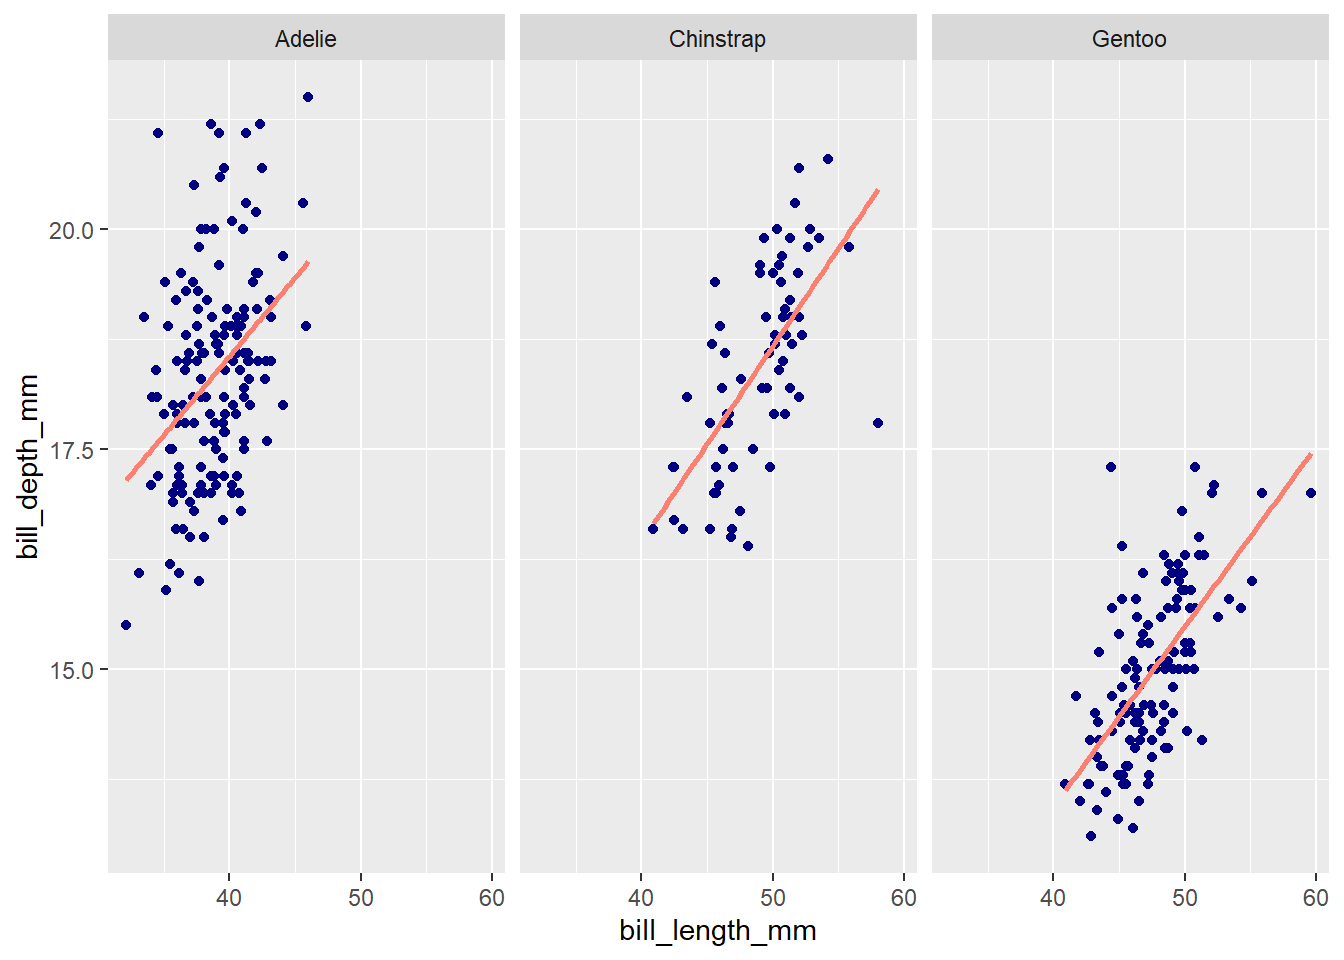
\includegraphics{_main_files/figure-latex/unnamed-chunk-292-1.pdf}

\begin{Shaded}
\begin{Highlighting}[]
\SpecialCharTok{\textgreater{}} \CommentTok{\# Use formula notation, a character vector, or vars() to specify faceting}
\ErrorTok{\textgreater{}} \CommentTok{\# variables; e.g., \textasciitilde{}species, c(\textquotesingle{}species\textquotesingle{}), or vars(species)}
\end{Highlighting}
\end{Shaded}

The number of rows and columns can be manually specified with \texttt{nrow} and \texttt{ncol} arguments in \texttt{facet\_wrap()}. By default, the x and y axes of all facet plots will be on the same scale. The axis ranges can be set to vary freely by adding \texttt{scales\ =\ \textquotesingle{}free\textquotesingle{}} as an argument (or, alternatively, \texttt{scales\ =\ \textquotesingle{}free\_x\textquotesingle{}} or \texttt{scales\ =\ \textquotesingle{}free\_y\textquotesingle{}} to free just the x or y axis).

Both \texttt{facet\_wrap()} and \texttt{facet\_grid()} can be used to make facet plots. When faceting based on multiple variables (e.g., species and sex), \texttt{facet\_wrap()} will drop group combinations for which there are no data points, whereas \texttt{facet\_grid()} will generate a plot for all possible group combinations:

\begin{Shaded}
\begin{Highlighting}[]
\SpecialCharTok{\textgreater{}} \FunctionTok{ggplot}\NormalTok{(penguins, }\FunctionTok{aes}\NormalTok{(}\AttributeTok{x =}\NormalTok{ bill\_length\_mm, }\AttributeTok{y =}\NormalTok{ bill\_depth\_mm)) }\SpecialCharTok{+}
\SpecialCharTok{+}   \FunctionTok{geom\_point}\NormalTok{(}\AttributeTok{color =} \StringTok{\textquotesingle{}navy\textquotesingle{}}\NormalTok{) }\SpecialCharTok{+}
\SpecialCharTok{+}   \FunctionTok{geom\_smooth}\NormalTok{(}\AttributeTok{method =} \StringTok{\textquotesingle{}lm\textquotesingle{}}\NormalTok{, }\AttributeTok{se =}\NormalTok{ F, }\AttributeTok{color =} \StringTok{\textquotesingle{}salmon\textquotesingle{}}\NormalTok{) }\SpecialCharTok{+}
\SpecialCharTok{+}   \FunctionTok{facet\_wrap}\NormalTok{(}\FunctionTok{vars}\NormalTok{(species, sex))}
\StringTok{\textasciigrave{}}\AttributeTok{geom\_smooth()}\StringTok{\textasciigrave{}}\NormalTok{ using formula }\StringTok{\textquotesingle{}y \textasciitilde{} x\textquotesingle{}}
\end{Highlighting}
\end{Shaded}

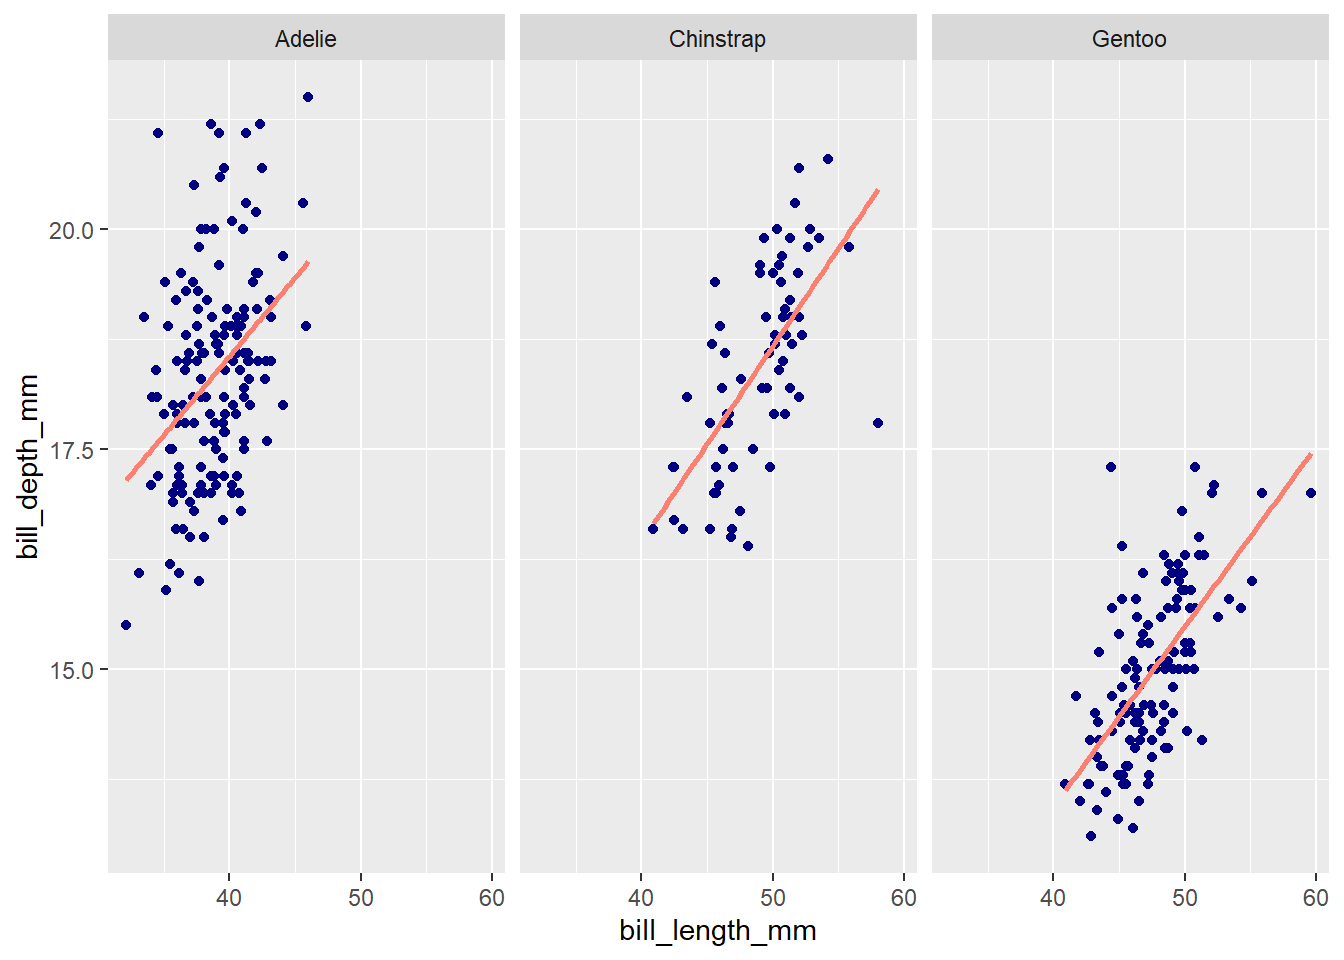
\includegraphics{_main_files/figure-latex/unnamed-chunk-293-1.pdf}

\begin{Shaded}
\begin{Highlighting}[]
\SpecialCharTok{\textgreater{}} 
\ErrorTok{\textgreater{}} \FunctionTok{ggplot}\NormalTok{(penguins, }\FunctionTok{aes}\NormalTok{(}\AttributeTok{x =}\NormalTok{ bill\_length\_mm, }\AttributeTok{y =}\NormalTok{ bill\_depth\_mm)) }\SpecialCharTok{+}
\SpecialCharTok{+}   \FunctionTok{geom\_point}\NormalTok{(}\AttributeTok{color =} \StringTok{\textquotesingle{}navy\textquotesingle{}}\NormalTok{) }\SpecialCharTok{+}
\SpecialCharTok{+}   \FunctionTok{geom\_smooth}\NormalTok{(}\AttributeTok{method =} \StringTok{\textquotesingle{}lm\textquotesingle{}}\NormalTok{, }\AttributeTok{se =}\NormalTok{ F, }\AttributeTok{color =} \StringTok{\textquotesingle{}salmon\textquotesingle{}}\NormalTok{) }\SpecialCharTok{+}
\SpecialCharTok{+}   \FunctionTok{facet\_grid}\NormalTok{(}\AttributeTok{rows =} \FunctionTok{vars}\NormalTok{(sex), }\AttributeTok{cols =} \FunctionTok{vars}\NormalTok{(species)) }
\StringTok{\textasciigrave{}}\AttributeTok{geom\_smooth()}\StringTok{\textasciigrave{}}\NormalTok{ using formula }\StringTok{\textquotesingle{}y \textasciitilde{} x\textquotesingle{}}
\end{Highlighting}
\end{Shaded}

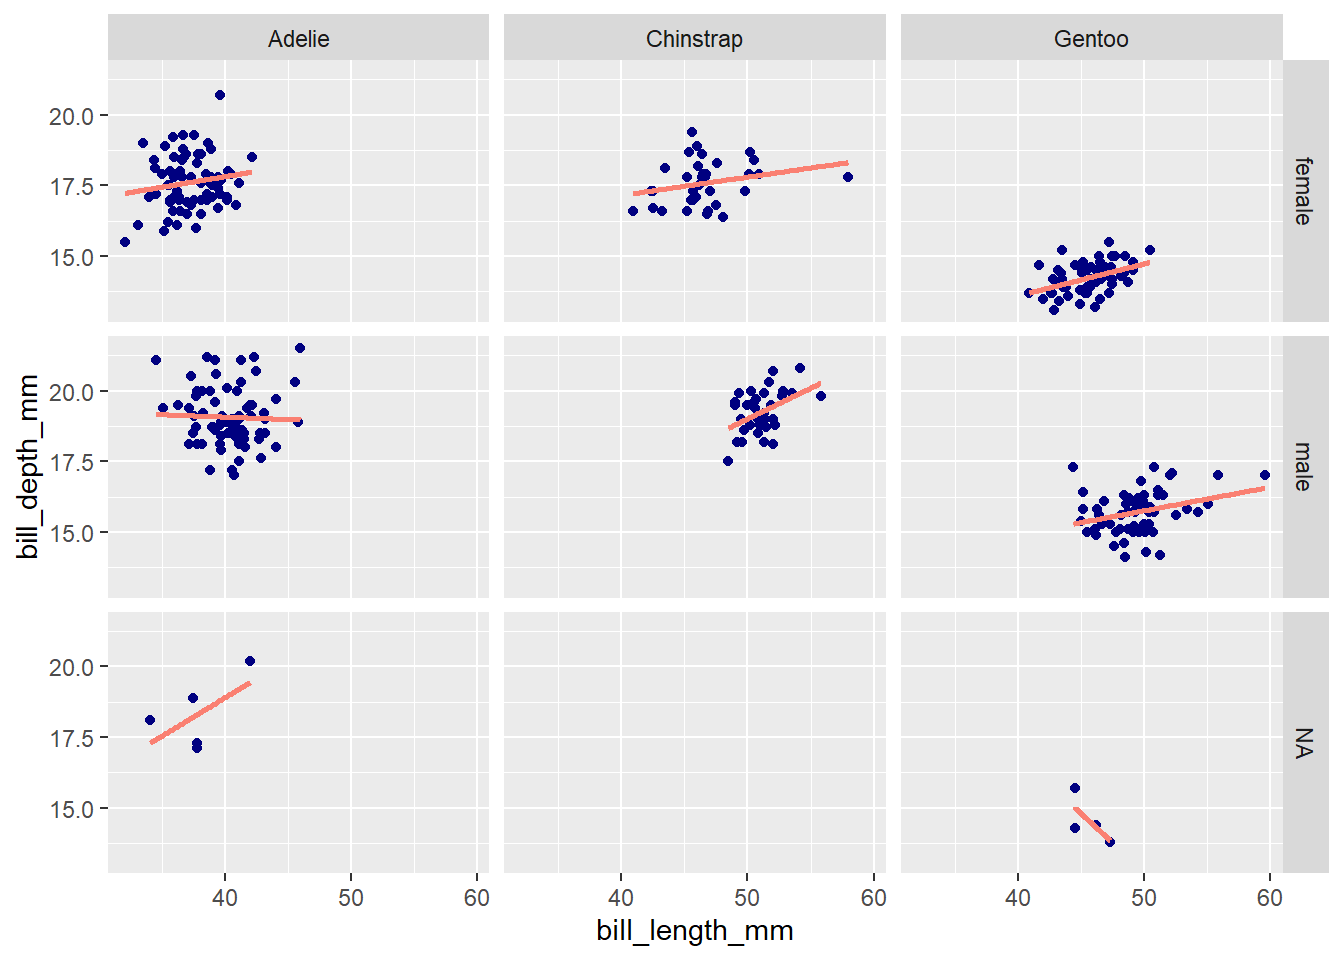
\includegraphics{_main_files/figure-latex/unnamed-chunk-293-2.pdf}

\begin{Shaded}
\begin{Highlighting}[]
\SpecialCharTok{\textgreater{}} \CommentTok{\# Note that facet\_grid() has separate \textasciigrave{}rows\textasciigrave{} and \textasciigrave{}cols\textasciigrave{} arguments for specifying}
\ErrorTok{\textgreater{}} \CommentTok{\# faceting variables}
\end{Highlighting}
\end{Shaded}

\hypertarget{selected-topics-in-statistical-inference}{%
\chapter{Selected Topics in Statistical Inference}\label{selected-topics-in-statistical-inference}}

This chapter looks at performing selected statistical analyses. It is not comprehensive. The focus is on implementation using Python and R. Good statistical practice is more than knowing which function to use. At a minimum we recommend reading the article, \href{https://journals.plos.org/ploscompbiol/article?id=10.1371/journal.pcbi.1004961}{Ten Simple Rules for Effective Statistical Practice} \citep{kass_caffo_davidian_meng_yu_reid_2016}.

\hypertarget{comparing-group-means}{%
\section{Comparing group means}\label{comparing-group-means}}

Many research studies compare mean values of some quantity of interest between two or more groups. A t test analyzes two group means. An Analysis of Variance, or ANOVA, analyzes three or more group means. Both the t test and ANOVA are special cases of a linear model.

To demonstrate the t test, we examine fictitious data on 15 scores between two groups of subjects. The ``control'' group was tested as-is while the ``treated'' group experienced a particular intervention. Of interest is (1) whether or not the mean scores differ meaningfully between the treated and control groups, and (2) if they do differ, how are they different?

To demonstrate the ANOVA test, we use data from \emph{The Analysis of Biological Data (3rd ed)}\citep{whitlock_schluter_2020} on the mass of pine cones (in grams) from three different environments in North America. Of interest is (1) whether or not the mean mass of pine cones differ meaningfully between the three locations, and (2) if they do differ, how are they different?

We usually assess the first question in each scenario with a hypothesis test and p-value. The null hypothesis is no difference between the means. The p-value is the probability of the observed differences between the groups (or more extreme differences) assuming the null hypothesis is true. A small p-value, traditionally less then 0.05, provides evidence against the null. For example, a p-value of 0.01 says there's a 1\% chance of sampling data as different as this (or more different) if there really was no difference between the groups. Note that p-values don't tell you how two or more statistics differ. See \href{https://www.tandfonline.com/doi/full/10.1080/00031305.2016.1154108\#_i28}{the ASA Statement on p-values}.

We assess the second question in each scenario by calculating confidence intervals on the difference in means. This is more informative than a p-value. A confidence interval gives us information on the uncertainty, direction and magnitude of a difference in means. For example, a 95\% confidence interval of {[}2, 15{]} tells us the data is consistent with a difference anywhere between 2 and 15 and that the mean of one group appears to be at least 2 units larger than the mean of the other group. Note that a 95\% confidence interval does not mean there is a 95\% probability that the true value is in the interval. The confidence interval either captured the true value or it did not. We don't know. However the \emph{process} of calculating the confidence interval works roughly 95\% of the time.

\hypertarget{python-47}{%
\subsubsection*{Python}\label{python-47}}
\addcontentsline{toc}{subsubsection}{Python}

\textbf{t-test}

Our data is available as a \textbf{Pandas} dataframe. It's small enough to view in its entirety.

\begin{Shaded}
\begin{Highlighting}[]
\OperatorTok{\textgreater{}}\NormalTok{ ch8\_d1}
\NormalTok{    score    group}
\DecValTok{0}    \FloatTok{77.0}\NormalTok{  control}
\DecValTok{1}    \FloatTok{81.0}\NormalTok{  control}
\DecValTok{2}    \FloatTok{77.0}\NormalTok{  control}
\DecValTok{3}    \FloatTok{86.0}\NormalTok{  control}
\DecValTok{4}    \FloatTok{81.0}\NormalTok{  control}
\DecValTok{5}    \FloatTok{77.0}\NormalTok{  control}
\DecValTok{6}    \FloatTok{82.0}\NormalTok{  control}
\DecValTok{7}    \FloatTok{83.0}\NormalTok{  control}
\DecValTok{8}    \FloatTok{82.0}\NormalTok{  control}
\DecValTok{9}    \FloatTok{79.0}\NormalTok{  control}
\DecValTok{10}   \FloatTok{86.0}\NormalTok{  control}
\DecValTok{11}   \FloatTok{82.0}\NormalTok{  control}
\DecValTok{12}   \FloatTok{78.0}\NormalTok{  control}
\DecValTok{13}   \FloatTok{71.0}\NormalTok{  control}
\DecValTok{14}   \FloatTok{84.0}\NormalTok{  control}
\DecValTok{15}   \FloatTok{85.0}\NormalTok{  treated}
\DecValTok{16}   \FloatTok{85.0}\NormalTok{  treated}
\DecValTok{17}   \FloatTok{89.0}\NormalTok{  treated}
\DecValTok{18}   \FloatTok{88.0}\NormalTok{  treated}
\DecValTok{19}   \FloatTok{87.0}\NormalTok{  treated}
\DecValTok{20}   \FloatTok{89.0}\NormalTok{  treated}
\DecValTok{21}   \FloatTok{88.0}\NormalTok{  treated}
\DecValTok{22}   \FloatTok{85.0}\NormalTok{  treated}
\DecValTok{23}   \FloatTok{77.0}\NormalTok{  treated}
\DecValTok{24}   \FloatTok{87.0}\NormalTok{  treated}
\DecValTok{25}   \FloatTok{85.0}\NormalTok{  treated}
\DecValTok{26}   \FloatTok{84.0}\NormalTok{  treated}
\DecValTok{27}   \FloatTok{79.0}\NormalTok{  treated}
\DecValTok{28}   \FloatTok{83.0}\NormalTok{  treated}
\DecValTok{29}   \FloatTok{87.0}\NormalTok{  treated}
\end{Highlighting}
\end{Shaded}

A stripchart is one of many ways to visualize numeric data between two groups. Here we use the seaborn function \texttt{stripplot()}. It appears the treated group had higher scores.

\begin{Shaded}
\begin{Highlighting}[]
\OperatorTok{\textgreater{}} \ImportTok{import}\NormalTok{ seaborn }\ImportTok{as}\NormalTok{ sns}
\OperatorTok{+} \ImportTok{import}\NormalTok{ matplotlib.pyplot }\ImportTok{as}\NormalTok{ plt}
\OperatorTok{+}\NormalTok{ plt.clf()}
\OperatorTok{+}\NormalTok{ sns.stripplot(x}\OperatorTok{=}\StringTok{"score"}\NormalTok{, y}\OperatorTok{=}\StringTok{"group"}\NormalTok{, data}\OperatorTok{=}\NormalTok{ch8\_d1)}
\OperatorTok{+}\NormalTok{ plt.show()}
\end{Highlighting}
\end{Shaded}

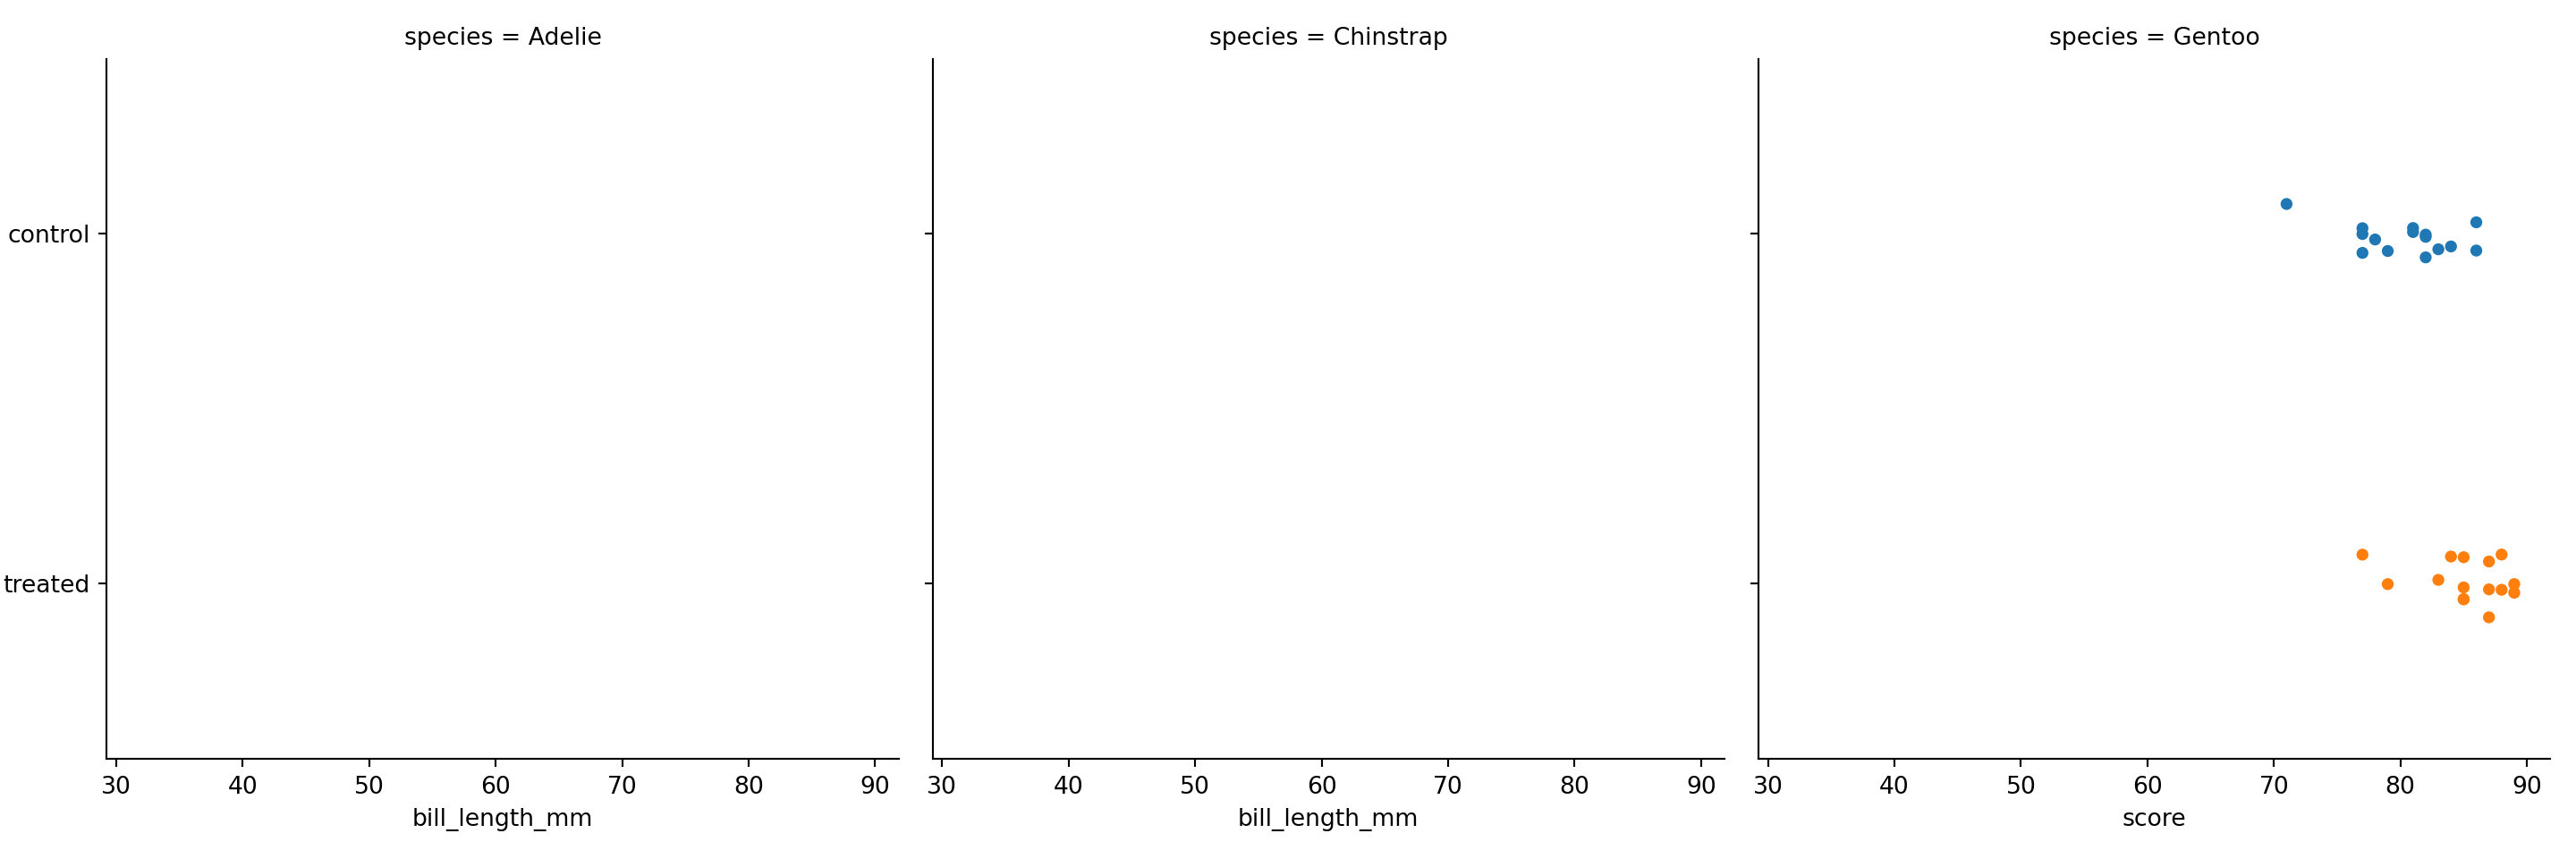
\includegraphics{_main_files/figure-latex/unnamed-chunk-298-1.pdf}

One way to perform a t test in Python is via the \texttt{CompareMeans()} function and its associated methods available in the \textbf{statsmodels} package. Below we import \textbf{statsmodels.stats.api} as ``sms''.

\begin{Shaded}
\begin{Highlighting}[]
\OperatorTok{\textgreater{}} \ImportTok{import}\NormalTok{ statsmodels.stats.api }\ImportTok{as}\NormalTok{ sms}
\end{Highlighting}
\end{Shaded}

We first extract the data we want to compare as pandas Series.

\begin{Shaded}
\begin{Highlighting}[]
\OperatorTok{\textgreater{}}\NormalTok{ d\_control }\OperatorTok{=}\NormalTok{ ch8\_d1.query(}\StringTok{\textquotesingle{}group == "control"\textquotesingle{}}\NormalTok{)[}\StringTok{\textquotesingle{}score\textquotesingle{}}\NormalTok{]}
\OperatorTok{+}\NormalTok{ d\_treated }\OperatorTok{=}\NormalTok{ ch8\_d1.query(}\StringTok{\textquotesingle{}group == "treated"\textquotesingle{}}\NormalTok{)[}\StringTok{\textquotesingle{}score\textquotesingle{}}\NormalTok{]}
\end{Highlighting}
\end{Shaded}

Next we create Descriptive statistics objects using the \texttt{DescrStatsW()} function.

\begin{Shaded}
\begin{Highlighting}[]
\OperatorTok{\textgreater{}}\NormalTok{ control }\OperatorTok{=}\NormalTok{ sms.DescrStatsW(d\_control)}
\OperatorTok{+}\NormalTok{ treated }\OperatorTok{=}\NormalTok{ sms.DescrStatsW(d\_treated)}
\end{Highlighting}
\end{Shaded}

Descriptive statistics objects have attributes such as \texttt{mean} and \texttt{std} (standard deviation). Below we print the mean and standard deviation of each group. We also round the standard deviation to three decimal places and place a line break before printing the standard deviation.

\begin{Shaded}
\begin{Highlighting}[]
\OperatorTok{\textgreater{}} \BuiltInTok{print}\NormalTok{(}\StringTok{"control mean:"}\NormalTok{, control.mean, }\StringTok{"}\CharTok{\textbackslash{}n}\StringTok{control std:"}\NormalTok{, }\BuiltInTok{round}\NormalTok{(control.std, }\DecValTok{3}\NormalTok{))}
\NormalTok{control mean: }\FloatTok{80.4} 
\NormalTok{control std: }\FloatTok{3.844}
\OperatorTok{\textgreater{}} \BuiltInTok{print}\NormalTok{(}\StringTok{"treated mean:"}\NormalTok{, treated.mean, }\StringTok{"}\CharTok{\textbackslash{}n}\StringTok{treated std:"}\NormalTok{, }\BuiltInTok{round}\NormalTok{(treated.std, }\DecValTok{3}\NormalTok{))}
\NormalTok{treated mean: }\FloatTok{85.2} 
\NormalTok{treated std: }\FloatTok{3.331}
\end{Highlighting}
\end{Shaded}

Next we create a CompareMeans means object using the \texttt{CompareMeans()} function. The required inputs are Descriptive statistics objects. We save the result as ``ttest''.

\begin{Shaded}
\begin{Highlighting}[]
\OperatorTok{\textgreater{}}\NormalTok{ ttest }\OperatorTok{=}\NormalTok{ sms.CompareMeans(control, treated)}
\end{Highlighting}
\end{Shaded}

Now we can use various methods with the ``ttest'' object. To see the result of a two sample t test assuming unequal variances, along with a confidence interval on the differences, use the \texttt{summary} method with \texttt{usevar=\textquotesingle{}unequal\textquotesingle{}}.

\begin{Shaded}
\begin{Highlighting}[]
\OperatorTok{\textgreater{}} \BuiltInTok{print}\NormalTok{(ttest.summary(usevar}\OperatorTok{=}\StringTok{\textquotesingle{}unequal\textquotesingle{}}\NormalTok{))}
\NormalTok{                          Test }\ControlFlowTok{for}\NormalTok{ equality of means                          }
\OperatorTok{==============================================================================}
\NormalTok{                 coef    std err          t      P}\OperatorTok{\textgreater{}|}\NormalTok{t}\OperatorTok{|}\NormalTok{      [}\FloatTok{0.025}      \FloatTok{0.975}\NormalTok{]}
\OperatorTok{{-}{-}{-}{-}{-}{-}{-}{-}{-}{-}{-}{-}{-}{-}{-}{-}{-}{-}{-}{-}{-}{-}{-}{-}{-}{-}{-}{-}{-}{-}{-}{-}{-}{-}{-}{-}{-}{-}{-}{-}{-}{-}{-}{-}{-}{-}{-}{-}{-}{-}{-}{-}{-}{-}{-}{-}{-}{-}{-}{-}{-}{-}{-}{-}{-}{-}{-}{-}{-}{-}{-}{-}{-}{-}{-}{-}{-}{-}}
\NormalTok{subset }\CommentTok{\#1     {-}4.8000      1.359     {-}3.531      0.001      {-}7.587      {-}2.013}
\OperatorTok{==============================================================================}
\end{Highlighting}
\end{Shaded}

The p-value of 0.001 is small, providing good evidence that the difference in means we witnessed reflects a real difference in the population. The confidence interval on the difference in means tells us the data is consistent with a difference between -7 and -2. It appears we can expect the control group to score at least 2 points lower than the treated group.

\textbf{ANOVA}

Our data is available as a \textbf{Pandas} dataframe. It's small enough to view in its entirety.

\begin{Shaded}
\begin{Highlighting}[]
\OperatorTok{\textgreater{}}\NormalTok{ ch8\_d2}
\NormalTok{    mass location}
\DecValTok{0}    \FloatTok{9.6}        \DecValTok{1}
\DecValTok{1}    \FloatTok{9.4}        \DecValTok{1}
\DecValTok{2}    \FloatTok{8.9}        \DecValTok{1}
\DecValTok{3}    \FloatTok{8.8}        \DecValTok{1}
\DecValTok{4}    \FloatTok{8.5}        \DecValTok{1}
\DecValTok{5}    \FloatTok{8.2}        \DecValTok{1}
\DecValTok{6}    \FloatTok{6.8}        \DecValTok{2}
\DecValTok{7}    \FloatTok{6.6}        \DecValTok{2}
\DecValTok{8}    \FloatTok{6.0}        \DecValTok{2}
\DecValTok{9}    \FloatTok{5.7}        \DecValTok{2}
\DecValTok{10}   \FloatTok{5.3}        \DecValTok{2}
\DecValTok{11}   \FloatTok{6.7}        \DecValTok{3}
\DecValTok{12}   \FloatTok{6.4}        \DecValTok{3}
\DecValTok{13}   \FloatTok{6.2}        \DecValTok{3}
\DecValTok{14}   \FloatTok{5.7}        \DecValTok{3}
\DecValTok{15}   \FloatTok{5.6}        \DecValTok{3}
\end{Highlighting}
\end{Shaded}

Again we use a stripchart to visualize the three groups of data. It appears the pine cones in location 1 have a higher mass.

\begin{Shaded}
\begin{Highlighting}[]
\OperatorTok{\textgreater{}}\NormalTok{ plt.clf()}
\OperatorTok{+}\NormalTok{ sns.stripplot(x}\OperatorTok{=}\StringTok{"mass"}\NormalTok{, y}\OperatorTok{=}\StringTok{"location"}\NormalTok{, data}\OperatorTok{=}\NormalTok{ch8\_d2)}
\OperatorTok{+}\NormalTok{ plt.show()}
\end{Highlighting}
\end{Shaded}

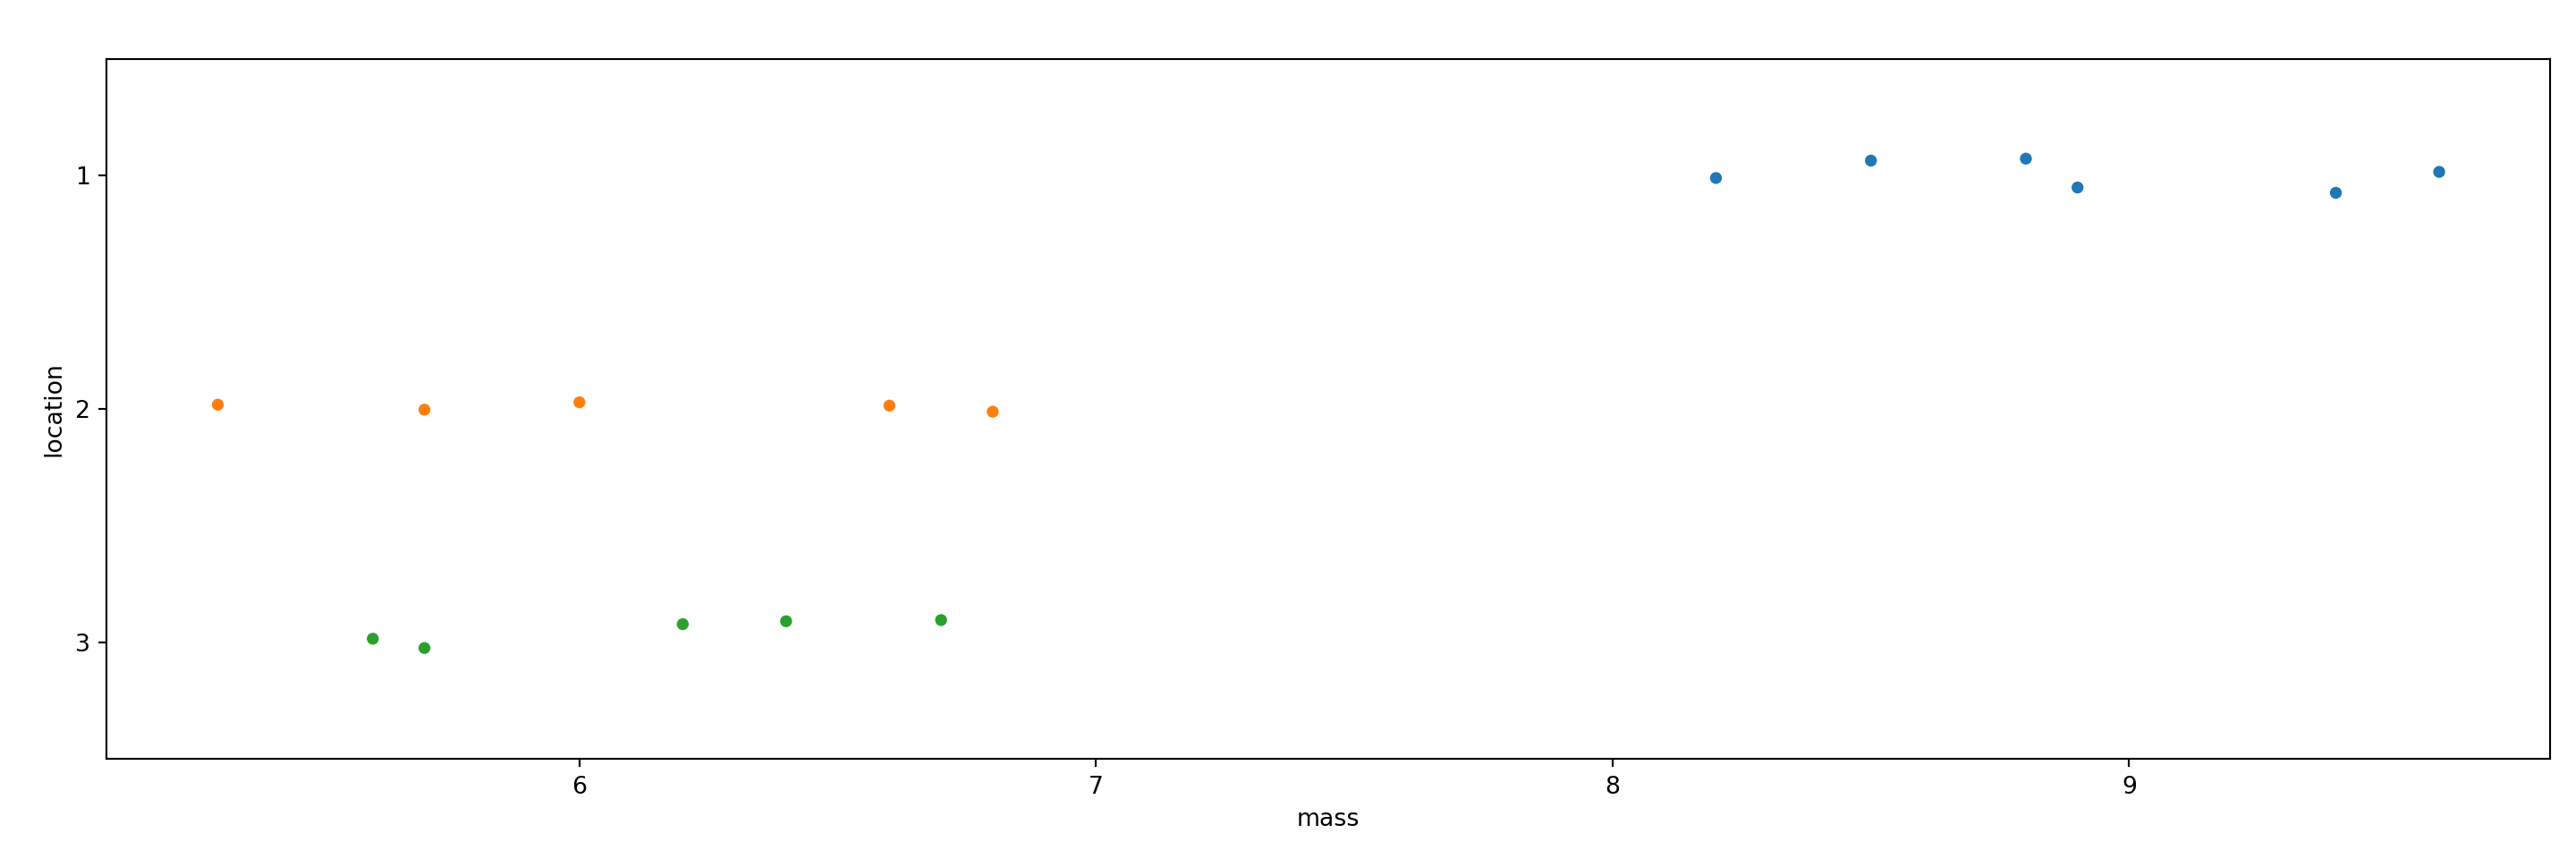
\includegraphics{_main_files/figure-latex/unnamed-chunk-306-3.pdf}

We can calculate means using the \texttt{groupby} and \texttt{mean} methods.

\begin{Shaded}
\begin{Highlighting}[]
\OperatorTok{\textgreater{}}\NormalTok{ ch8\_d2[}\StringTok{\textquotesingle{}mass\textquotesingle{}}\NormalTok{].groupby(ch8\_d2[}\StringTok{\textquotesingle{}location\textquotesingle{}}\NormalTok{]).mean()}
\NormalTok{location}
\DecValTok{1}    \FloatTok{8.90}
\DecValTok{2}    \FloatTok{6.08}
\DecValTok{3}    \FloatTok{6.12}
\NormalTok{Name: mass, dtype: float64}
\end{Highlighting}
\end{Shaded}

One way to perform an ANOVA test in Python is via the \texttt{anova\_oneway()} function, also available in the \textbf{statsmodels} package.

The \texttt{anova\_oneway()} function can perform an ANOVA on a pandas Dataframe with the first argument specifying the numeric data and the second argument the grouping variable. We also set \texttt{use\_var=\textquotesingle{}equal\textquotesingle{}} to replicate the R output below.

\begin{Shaded}
\begin{Highlighting}[]
\OperatorTok{\textgreater{}}\NormalTok{ sms.anova\_oneway(ch8\_d2.mass, ch8\_d2.location, use\_var}\OperatorTok{=}\StringTok{\textquotesingle{}equal\textquotesingle{}}\NormalTok{)}
\OperatorTok{\textless{}}\KeywordTok{class} \StringTok{\textquotesingle{}statsmodels.stats.base.HolderTuple\textquotesingle{}}\OperatorTok{\textgreater{}}
\NormalTok{statistic }\OperatorTok{=} \FloatTok{50.085429769392036}
\NormalTok{pvalue }\OperatorTok{=} \FloatTok{7.786760128813737e{-}07}
\NormalTok{df }\OperatorTok{=}\NormalTok{ (}\FloatTok{2.0}\NormalTok{, }\FloatTok{13.0}\NormalTok{)}
\NormalTok{df\_num }\OperatorTok{=} \FloatTok{2.0}
\NormalTok{df\_denom }\OperatorTok{=} \FloatTok{13.0}
\NormalTok{nobs\_t }\OperatorTok{=} \FloatTok{16.0}
\NormalTok{n\_groups }\OperatorTok{=} \DecValTok{3}
\NormalTok{means }\OperatorTok{=}\NormalTok{ array([}\FloatTok{8.9}\NormalTok{ , }\FloatTok{6.08}\NormalTok{, }\FloatTok{6.12}\NormalTok{])}
\NormalTok{nobs }\OperatorTok{=}\NormalTok{ array([}\FloatTok{6.}\NormalTok{, }\FloatTok{5.}\NormalTok{, }\FloatTok{5.}\NormalTok{])}
\NormalTok{vars\_ }\OperatorTok{=}\NormalTok{ array([}\FloatTok{0.28}\NormalTok{ , }\FloatTok{0.387}\NormalTok{, }\FloatTok{0.217}\NormalTok{])}
\NormalTok{use\_var }\OperatorTok{=} \StringTok{\textquotesingle{}equal\textquotesingle{}}
\NormalTok{welch\_correction }\OperatorTok{=} \VariableTok{True}
\BuiltInTok{tuple} \OperatorTok{=}\NormalTok{ (}\FloatTok{50.085429769392036}\NormalTok{, }\FloatTok{7.786760128813737e{-}07}\NormalTok{)}
\end{Highlighting}
\end{Shaded}

The small p-value of 0.0000007 provides strong evidence that the difference in means we witnessed reflects a real difference in the population.

A common follow-up to an ANOVA is Tukey's Honestly Significant Differences (HSD), which computes differences between all possible pairs and returns adjusted p-values and confidence intervals to account for the multiple comparisons. To carry this out in the \textbf{statsmodels} package, we need to first create a MultiComparison object using the \texttt{multicomp.MultiComparison()} function. Then we use the \texttt{tukeyhsd()} method to compare the means with corrected p-values.

\begin{Shaded}
\begin{Highlighting}[]
\OperatorTok{\textgreater{}}\NormalTok{ mc }\OperatorTok{=}\NormalTok{ sms.multicomp.MultiComparison(ch8\_d2.mass, ch8\_d2.location)}
\OperatorTok{+} \BuiltInTok{print}\NormalTok{(mc.tukeyhsd())}
\NormalTok{Multiple Comparison of Means }\OperatorTok{{-}}\NormalTok{ Tukey HSD, FWER}\OperatorTok{=}\FloatTok{0.05} 
\OperatorTok{====================================================}
\NormalTok{group1 group2 meandiff p}\OperatorTok{{-}}\NormalTok{adj   lower   upper  reject}
\OperatorTok{{-}{-}{-}{-}{-}{-}{-}{-}{-}{-}{-}{-}{-}{-}{-}{-}{-}{-}{-}{-}{-}{-}{-}{-}{-}{-}{-}{-}{-}{-}{-}{-}{-}{-}{-}{-}{-}{-}{-}{-}{-}{-}{-}{-}{-}{-}{-}{-}{-}{-}{-}{-}}
     \DecValTok{1}      \DecValTok{2}    \OperatorTok{{-}}\FloatTok{2.82}    \FloatTok{0.0} \OperatorTok{{-}}\FloatTok{3.6863} \OperatorTok{{-}}\FloatTok{1.9537}   \VariableTok{True}
     \DecValTok{1}      \DecValTok{3}    \OperatorTok{{-}}\FloatTok{2.78}    \FloatTok{0.0} \OperatorTok{{-}}\FloatTok{3.6463} \OperatorTok{{-}}\FloatTok{1.9137}   \VariableTok{True}
     \DecValTok{2}      \DecValTok{3}     \FloatTok{0.04} \FloatTok{0.9925} \OperatorTok{{-}}\FloatTok{0.8648}  \FloatTok{0.9448}  \VariableTok{False}
\OperatorTok{{-}{-}{-}{-}{-}{-}{-}{-}{-}{-}{-}{-}{-}{-}{-}{-}{-}{-}{-}{-}{-}{-}{-}{-}{-}{-}{-}{-}{-}{-}{-}{-}{-}{-}{-}{-}{-}{-}{-}{-}{-}{-}{-}{-}{-}{-}{-}{-}{-}{-}{-}{-}}
\end{Highlighting}
\end{Shaded}

The difference in means between locations 2 and 1 (2 - 1) and locations 3 and 1 (3 - 1) are about -2.8. The difference in means between locations 3 and 2 (3 - 2) is inconclusive. It seems to be small but we're not sure if the difference is positive or negative.

\hypertarget{r-47}{%
\subsubsection*{R}\label{r-47}}
\addcontentsline{toc}{subsubsection}{R}

\textbf{t-test}

The \texttt{str()} function allows to take a quick look at the data frame \texttt{ch8\_d1}. One column contains the scores, the other column indicates which group the subject was in (control vs treated).

\begin{Shaded}
\begin{Highlighting}[]
\SpecialCharTok{\textgreater{}} \FunctionTok{str}\NormalTok{(ch8\_d1)}
\StringTok{\textquotesingle{}data.frame\textquotesingle{}}\SpecialCharTok{:}   \DecValTok{30}\NormalTok{ obs. of  }\DecValTok{2}\NormalTok{ variables}\SpecialCharTok{:}
 \ErrorTok{$}\NormalTok{ score}\SpecialCharTok{:}\NormalTok{ num  }\DecValTok{77} \DecValTok{81} \DecValTok{77} \DecValTok{86} \DecValTok{81} \DecValTok{77} \DecValTok{82} \DecValTok{83} \DecValTok{82} \DecValTok{79}\NormalTok{ ...}
 \SpecialCharTok{$}\NormalTok{ group}\SpecialCharTok{:}\NormalTok{ chr  }\StringTok{"control"} \StringTok{"control"} \StringTok{"control"} \StringTok{"control"}\NormalTok{ ...}
\end{Highlighting}
\end{Shaded}

A stripchart is one of many ways to visualize numeric data between two groups. Here we use the base R function \texttt{stripchart()}. The formula \texttt{score\ \textasciitilde{}\ group} says to plot score by group. The \texttt{las\ =\ 1} argument says to rotate the y-axis labels. The \texttt{method\ =\ "jitter"} arguments says to randomly scatter the points vertically so they don't overplot. It appears the treated group had higher scores.

\begin{Shaded}
\begin{Highlighting}[]
\SpecialCharTok{\textgreater{}} \FunctionTok{stripchart}\NormalTok{(score }\SpecialCharTok{\textasciitilde{}}\NormalTok{ group, }\AttributeTok{data =}\NormalTok{ ch8\_d1, }\AttributeTok{las =} \DecValTok{1}\NormalTok{, }\AttributeTok{method =} \StringTok{"jitter"}\NormalTok{)}
\end{Highlighting}
\end{Shaded}

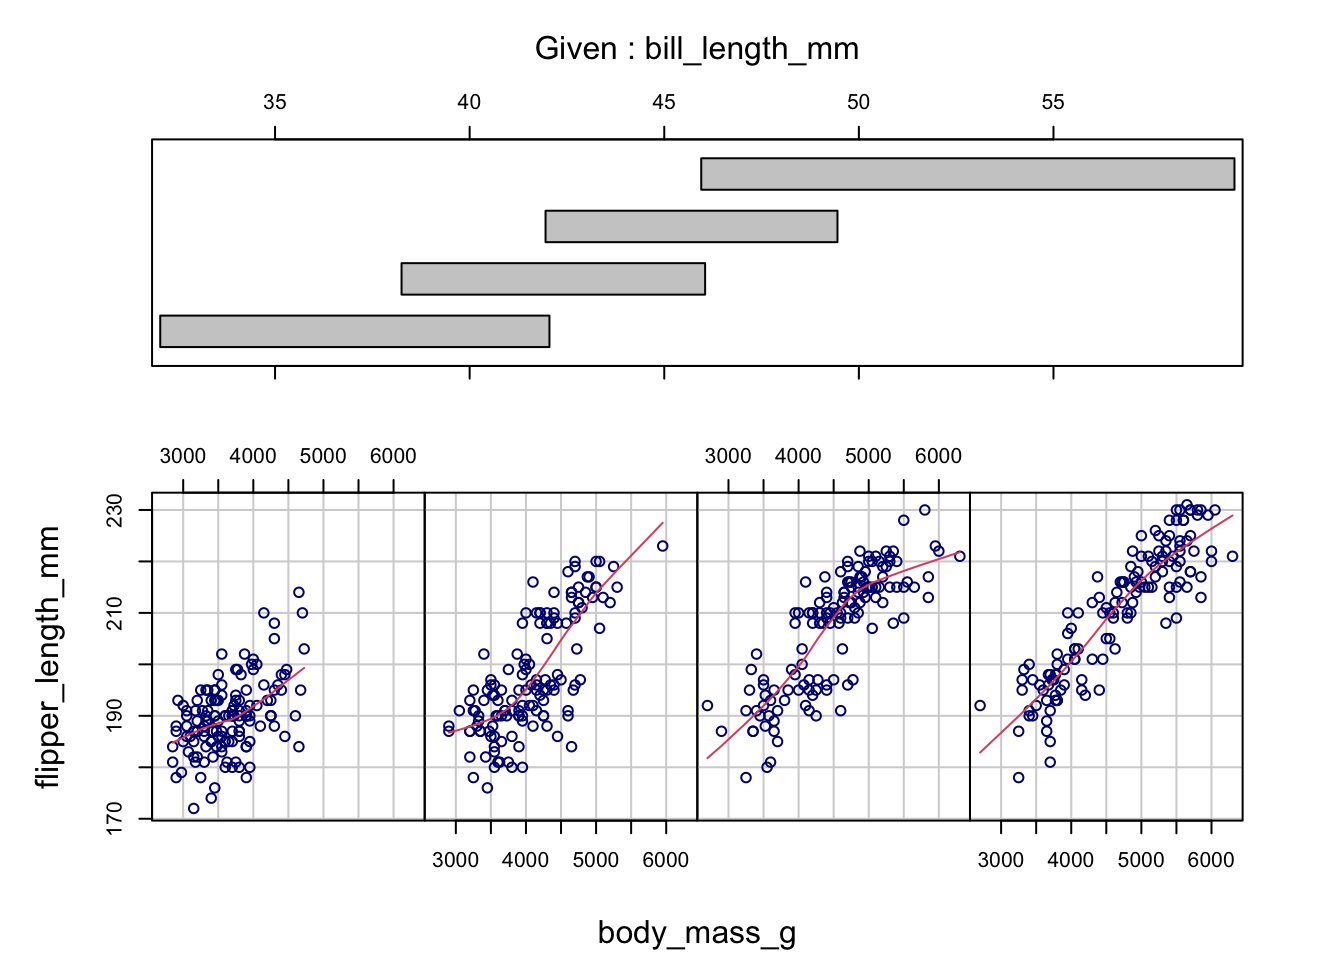
\includegraphics{_main_files/figure-latex/unnamed-chunk-311-1.pdf}

To calculate the means between the two groups we can use the \texttt{aggregate()} function. Again the formula \texttt{score\ \textasciitilde{}\ group} says to aggregate score by group. We specify \texttt{mean} so that we calculate the mean between the two groups. Some other functions we could specify include \texttt{median}, \texttt{sd}, or \texttt{sum}. The sample mean of the treated group is about 5 points higher than the control group.

\begin{Shaded}
\begin{Highlighting}[]
\SpecialCharTok{\textgreater{}} \FunctionTok{aggregate}\NormalTok{(score }\SpecialCharTok{\textasciitilde{}}\NormalTok{ group, }\AttributeTok{data =}\NormalTok{ ch8\_d1, mean)}
\NormalTok{    group score}
\DecValTok{1}\NormalTok{ control  }\FloatTok{80.4}
\DecValTok{2}\NormalTok{ treated  }\FloatTok{85.2}
\end{Highlighting}
\end{Shaded}

Is this difference meaningful? What if we took more samples? Would each sample result in similar differences in the means? A t test attempts to answer this.

The \texttt{t.test()} function accommodates formula notation allowing us to specify that we want to calculate mean score by group.

\begin{Shaded}
\begin{Highlighting}[]
\SpecialCharTok{\textgreater{}} \FunctionTok{t.test}\NormalTok{(score }\SpecialCharTok{\textasciitilde{}}\NormalTok{ group, }\AttributeTok{data =}\NormalTok{ ch8\_d1)}

\NormalTok{    Welch Two Sample t}\SpecialCharTok{{-}}\NormalTok{test}

\NormalTok{data}\SpecialCharTok{:}\NormalTok{  score by group}
\NormalTok{t }\OtherTok{=} \SpecialCharTok{{-}}\FloatTok{3.5313}\NormalTok{, df }\OtherTok{=} \FloatTok{27.445}\NormalTok{, p}\SpecialCharTok{{-}}\NormalTok{value }\OtherTok{=} \FloatTok{0.001482}
\NormalTok{alternative hypothesis}\SpecialCharTok{:}\NormalTok{ true difference }\ControlFlowTok{in}\NormalTok{ means between group control and group treated is not equal to }\DecValTok{0}
\DecValTok{95}\NormalTok{ percent confidence interval}\SpecialCharTok{:}
 \SpecialCharTok{{-}}\FloatTok{7.586883} \SpecialCharTok{{-}}\FloatTok{2.013117}
\NormalTok{sample estimates}\SpecialCharTok{:}
\NormalTok{mean }\ControlFlowTok{in}\NormalTok{ group control mean }\ControlFlowTok{in}\NormalTok{ group treated }
                 \FloatTok{80.4}                  \FloatTok{85.2} 
\end{Highlighting}
\end{Shaded}

The p-value of 0.0015 is small, providing good evidence that the difference in means we witnessed reflects a real difference in the population. The confidence interval on the difference in means tells us the data is consistent with a difference between -7 and -2. It appears we can expect the control group to score at least 2 points lower than the treated group.

\textbf{ANOVA}

The \texttt{str()} function allows to take a quick look at the data frame \texttt{ch8\_d2}. One column contains the mass of the pine cones, the other column indicates which location the pine cone was found.

\begin{Shaded}
\begin{Highlighting}[]
\SpecialCharTok{\textgreater{}} \FunctionTok{str}\NormalTok{(ch8\_d2)}
\StringTok{\textquotesingle{}data.frame\textquotesingle{}}\SpecialCharTok{:}   \DecValTok{16}\NormalTok{ obs. of  }\DecValTok{2}\NormalTok{ variables}\SpecialCharTok{:}
 \ErrorTok{$}\NormalTok{ mass    }\SpecialCharTok{:}\NormalTok{ num  }\FloatTok{9.6} \FloatTok{9.4} \FloatTok{8.9} \FloatTok{8.8} \FloatTok{8.5} \FloatTok{8.2} \FloatTok{6.8} \FloatTok{6.6} \DecValTok{6} \FloatTok{5.7}\NormalTok{ ...}
 \SpecialCharTok{$}\NormalTok{ location}\SpecialCharTok{:}\NormalTok{ chr  }\StringTok{"1"} \StringTok{"1"} \StringTok{"1"} \StringTok{"1"}\NormalTok{ ...}
\end{Highlighting}
\end{Shaded}

Again we use a stripchart to visualize the three groups of data. It appears the pine cones in location 1 have a higher mass.

\begin{Shaded}
\begin{Highlighting}[]
\SpecialCharTok{\textgreater{}} \FunctionTok{stripchart}\NormalTok{(mass }\SpecialCharTok{\textasciitilde{}}\NormalTok{ location, }\AttributeTok{data =}\NormalTok{ ch8\_d2, }\AttributeTok{las =} \DecValTok{1}\NormalTok{, }\AttributeTok{method =} \StringTok{"jitter"}\NormalTok{)}
\end{Highlighting}
\end{Shaded}

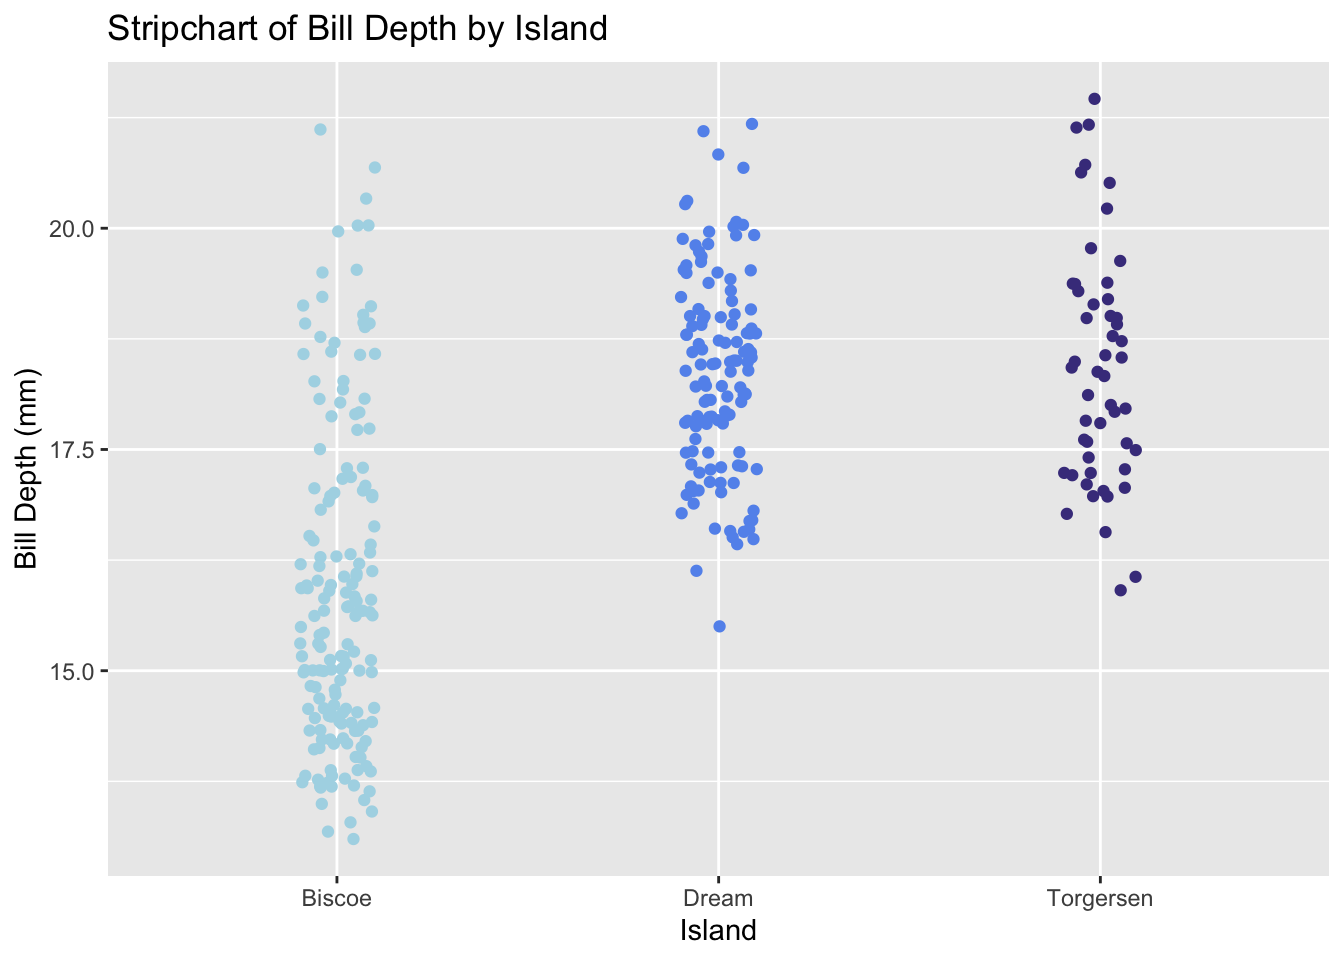
\includegraphics{_main_files/figure-latex/unnamed-chunk-315-1.pdf}

To calculate the means between the three groups we can use the \texttt{aggregate()} function. Again the formula \texttt{mass\ \textasciitilde{}\ location} says to aggregate mass by location. We specify \texttt{mean} so that we calculate the mean between the three groups.

\begin{Shaded}
\begin{Highlighting}[]
\SpecialCharTok{\textgreater{}} \FunctionTok{aggregate}\NormalTok{(mass }\SpecialCharTok{\textasciitilde{}}\NormalTok{ location, }\AttributeTok{data =}\NormalTok{ ch8\_d2, mean)}
\NormalTok{  location mass}
\DecValTok{1}        \DecValTok{1} \FloatTok{8.90}
\DecValTok{2}        \DecValTok{2} \FloatTok{6.08}
\DecValTok{3}        \DecValTok{3} \FloatTok{6.12}
\end{Highlighting}
\end{Shaded}

Is this difference meaningful? ANOVA attempts to answer this.

The \texttt{aov()} function carries out the ANOVA test and also accommodates formula notation. It's usually preferable to save the ANOVA result into an object and call \texttt{summary()} on the object.

\begin{Shaded}
\begin{Highlighting}[]
\SpecialCharTok{\textgreater{}}\NormalTok{ aov1 }\OtherTok{\textless{}{-}} \FunctionTok{aov}\NormalTok{(mass }\SpecialCharTok{\textasciitilde{}}\NormalTok{ location, }\AttributeTok{data =}\NormalTok{ ch8\_d2)}
\SpecialCharTok{\textgreater{}} \FunctionTok{summary}\NormalTok{(aov1)}
\NormalTok{            Df Sum Sq Mean Sq F value   }\FunctionTok{Pr}\NormalTok{(}\SpecialCharTok{\textgreater{}}\NormalTok{F)    }
\NormalTok{location     }\DecValTok{2} \FloatTok{29.404}  \FloatTok{14.702}   \FloatTok{50.09} \FloatTok{7.79e{-}07} \SpecialCharTok{**}\ErrorTok{*}
\NormalTok{Residuals   }\DecValTok{13}  \FloatTok{3.816}   \FloatTok{0.294}                     
\SpecialCharTok{{-}{-}{-}}
\NormalTok{Signif. codes}\SpecialCharTok{:}  \DecValTok{0} \StringTok{\textquotesingle{}***\textquotesingle{}} \FloatTok{0.001} \StringTok{\textquotesingle{}**\textquotesingle{}} \FloatTok{0.01} \StringTok{\textquotesingle{}*\textquotesingle{}} \FloatTok{0.05} \StringTok{\textquotesingle{}.\textquotesingle{}} \FloatTok{0.1} \StringTok{\textquotesingle{} \textquotesingle{}} \DecValTok{1}
\end{Highlighting}
\end{Shaded}

The small p-value of 0.0000007 provides strong evidence that the difference in means we witnessed reflects a real difference in the population.

Unlike the \texttt{t.test()} output, the \texttt{aov()} summary does not provide confidence intervals on differences in means. That's because there are many kinds of differences we might want to assess. A common and easy procedure is Tukey's Honestly Significant Differences (HSD), which computes differences between all possible pairs and returns adjusted p-values and confidence intervals to account for the multiple comparisons. Base R provides the \texttt{TukeyHSD()} function for this task. Call it on the ANOVA object.

\begin{Shaded}
\begin{Highlighting}[]
\SpecialCharTok{\textgreater{}} \FunctionTok{TukeyHSD}\NormalTok{(aov1)}
\NormalTok{  Tukey multiple comparisons of means}
    \DecValTok{95}\NormalTok{\% family}\SpecialCharTok{{-}}\NormalTok{wise confidence level}

\NormalTok{Fit}\SpecialCharTok{:} \FunctionTok{aov}\NormalTok{(}\AttributeTok{formula =}\NormalTok{ mass }\SpecialCharTok{\textasciitilde{}}\NormalTok{ location, }\AttributeTok{data =}\NormalTok{ ch8\_d2)}

\SpecialCharTok{$}\NormalTok{location}
\NormalTok{     diff        lwr        upr     p adj}
\DecValTok{2{-}1} \SpecialCharTok{{-}}\FloatTok{2.82} \SpecialCharTok{{-}}\FloatTok{3.6862516} \SpecialCharTok{{-}}\FloatTok{1.9537484} \FloatTok{0.0000028}
\DecValTok{3{-}1} \SpecialCharTok{{-}}\FloatTok{2.78} \SpecialCharTok{{-}}\FloatTok{3.6462516} \SpecialCharTok{{-}}\FloatTok{1.9137484} \FloatTok{0.0000033}
\DecValTok{3{-}2}  \FloatTok{0.04} \SpecialCharTok{{-}}\FloatTok{0.8647703}  \FloatTok{0.9447703} \FloatTok{0.9925198}
\end{Highlighting}
\end{Shaded}

The difference in means between locations 2 and 1 (2 - 1) and locations 3 and 1 (3 - 1) are about -2.8. The difference in means between locations 3 and 2 (3 - 2) is inconclusive. It seems to be small but we're not sure if the difference is positive or negative.

\hypertarget{comparing-group-proportions}{%
\section{Comparing group proportions}\label{comparing-group-proportions}}

It is often of interest to compare proportions between two groups. Sometimes this is referred to as a two-sample proportion test. To demonstrate we use an exercise from the text \emph{Introductory Statistics with R} \citep{Dalgaard_2020} (p.154). We are told that 210 out of 747 patients died of Rocky Mountain spotted fever in the western United States. That's a proportion of 0.281. In the eastern United States, 122 out 661 patients died. That's a proportion of 0.185. Is the difference in proportions statistically significant? In other words, assuming there is no difference in the fatality rate between the two regions, is this difference in proportions surprising?

\hypertarget{python-48}{%
\subsubsection*{Python}\label{python-48}}
\addcontentsline{toc}{subsubsection}{Python}

A two-sample proportion test can be carried out in Python using the \texttt{test\_proportions\_2indep()} function from the \textbf{statsmodels} package. The two proportions being compared must be independent.

The first argument is the number of successes or occurrences for the first proportion. The second argument is the number of total trials for the first group. The third and fourth arguments are the occurrences and total number of trials for the second group, respectively.

\begin{Shaded}
\begin{Highlighting}[]
\OperatorTok{\textgreater{}} \ImportTok{import}\NormalTok{ statsmodels.stats.api }\ImportTok{as}\NormalTok{ sms}
\OperatorTok{+}\NormalTok{ ptest }\OperatorTok{=}\NormalTok{ sms.test\_proportions\_2indep(}\DecValTok{210}\NormalTok{, }\DecValTok{747}\NormalTok{, }\DecValTok{122}\NormalTok{, }\DecValTok{661}\NormalTok{)}
\end{Highlighting}
\end{Shaded}

We can extract the p-value of the test and the difference in proportions using the \texttt{pvalue} and \texttt{diff} attributes, respectively.

\begin{Shaded}
\begin{Highlighting}[]
\OperatorTok{\textgreater{}}\NormalTok{ ptest.pvalue}
\FloatTok{1.632346798072468e{-}05}
\end{Highlighting}
\end{Shaded}

\begin{Shaded}
\begin{Highlighting}[]
\OperatorTok{\textgreater{}} \CommentTok{\# rounded to 4 decimal places}
\OperatorTok{+} \BuiltInTok{round}\NormalTok{(ptest.diff, }\DecValTok{4}\NormalTok{)}
\FloatTok{0.0966}
\end{Highlighting}
\end{Shaded}

To calculate a 95\% confidence interval for the difference in proportions we need to use the \texttt{confint\_proportions\_2indep()} function.

\begin{Shaded}
\begin{Highlighting}[]
\OperatorTok{\textgreater{}}\NormalTok{ pdiff }\OperatorTok{=}\NormalTok{ sms.confint\_proportions\_2indep(}\DecValTok{210}\NormalTok{, }\DecValTok{747}\NormalTok{, }\DecValTok{122}\NormalTok{, }\DecValTok{661}\NormalTok{)}
\OperatorTok{+}\NormalTok{ pdiff}
\NormalTok{(}\FloatTok{0.05241555145475882}\NormalTok{, }\FloatTok{0.13988087590630482}\NormalTok{)}
\end{Highlighting}
\end{Shaded}

The result is returned as a tuple with an extreme amount of precision. We recommend rounding these values to few decimal places. Here's one way using f strings. Notice we extract each element of the ``pdiff'' tuple and round to 5 decimal places.

\begin{Shaded}
\begin{Highlighting}[]
\OperatorTok{\textgreater{}} \BuiltInTok{print}\NormalTok{(}\SpecialStringTok{f"(}\SpecialCharTok{\{}\BuiltInTok{round}\NormalTok{(pdiff[}\DecValTok{0}\NormalTok{],}\DecValTok{5}\NormalTok{)}\SpecialCharTok{\}}\SpecialStringTok{, }\SpecialCharTok{\{}\BuiltInTok{round}\NormalTok{(pdiff[}\DecValTok{1}\NormalTok{],}\DecValTok{5}\NormalTok{)}\SpecialCharTok{\}}\SpecialStringTok{)"}\NormalTok{)}
\NormalTok{(}\FloatTok{0.05242}\NormalTok{, }\FloatTok{0.13988}\NormalTok{)}
\end{Highlighting}
\end{Shaded}

This results are slightly different from the R example below. That's because the \texttt{test\_proportions\_2indep()} and \texttt{confint\_proportions\_2indep()} functions use different methods. See their respective help pages to learn more about the methods available and other function arguments.

\href{https://www.statsmodels.org/dev/generated/statsmodels.stats.proportion.test_proportions_2indep.html\#statsmodels.stats.proportion.test_proportions_2indep}{test\_proportions\_2indep} help page\\
\href{https://www.statsmodels.org/dev/generated/statsmodels.stats.proportion.confint_proportions_2indep.html\#statsmodels.stats.proportion.confint_proportions_2indep}{confint\_proportions\_2indep} help page

\hypertarget{r-48}{%
\subsubsection*{R}\label{r-48}}
\addcontentsline{toc}{subsubsection}{R}

A two-sample proportion test in R can be carried out with the \texttt{prop.test()} function. The first argument, \texttt{x}, is the number of ``successes'' or ``occurrences'' of some event for each group. The second argument, \texttt{n}, is the number of total trials for each group.

\begin{Shaded}
\begin{Highlighting}[]
\SpecialCharTok{\textgreater{}} \FunctionTok{prop.test}\NormalTok{(}\AttributeTok{x =} \FunctionTok{c}\NormalTok{(}\DecValTok{210}\NormalTok{, }\DecValTok{122}\NormalTok{), }\AttributeTok{n =} \FunctionTok{c}\NormalTok{(}\DecValTok{747}\NormalTok{, }\DecValTok{661}\NormalTok{))}

    \DecValTok{2}\SpecialCharTok{{-}}\NormalTok{sample test }\ControlFlowTok{for}\NormalTok{ equality of proportions with continuity correction}

\NormalTok{data}\SpecialCharTok{:}  \FunctionTok{c}\NormalTok{(}\DecValTok{210}\NormalTok{, }\DecValTok{122}\NormalTok{) out of }\FunctionTok{c}\NormalTok{(}\DecValTok{747}\NormalTok{, }\DecValTok{661}\NormalTok{)}
\NormalTok{X}\SpecialCharTok{{-}}\NormalTok{squared }\OtherTok{=} \FloatTok{17.612}\NormalTok{, df }\OtherTok{=} \DecValTok{1}\NormalTok{, p}\SpecialCharTok{{-}}\NormalTok{value }\OtherTok{=} \FloatTok{2.709e{-}05}
\NormalTok{alternative hypothesis}\SpecialCharTok{:}\NormalTok{ two.sided}
\DecValTok{95}\NormalTok{ percent confidence interval}\SpecialCharTok{:}
 \FloatTok{0.05138139} \FloatTok{0.14172994}
\NormalTok{sample estimates}\SpecialCharTok{:}
\NormalTok{   prop }\DecValTok{1}\NormalTok{    prop }\DecValTok{2} 
\FloatTok{0.2811245} \FloatTok{0.1845688} 
\end{Highlighting}
\end{Shaded}

The proportion of patients who died in the western US is about 0.28. The proportion who died in the eastern US is about 0.18. The small p-value says there is a very small chance of seeing a difference as large as this (or larger) if there really was no difference in the proportions. The confidence interval on the difference of proportions ranges from 0.05 to 0.14, indicating that this fever seems to kill at least 5\% more patients in the western US.

Sometimes data is presented in a 2-way table with successes and failures. We can present the preceding data in a table as follows using the \texttt{matrix()} function.

\begin{Shaded}
\begin{Highlighting}[]
\SpecialCharTok{\textgreater{}}\NormalTok{ fever }\OtherTok{\textless{}{-}} \FunctionTok{matrix}\NormalTok{(}\FunctionTok{c}\NormalTok{(}\DecValTok{210}\NormalTok{, }\DecValTok{122}\NormalTok{,}
\SpecialCharTok{+}                   \DecValTok{747{-}210}\NormalTok{, }\DecValTok{661{-}122}\NormalTok{), }\AttributeTok{ncol =} \DecValTok{2}\NormalTok{)}
\SpecialCharTok{\textgreater{}} \FunctionTok{rownames}\NormalTok{(fever) }\OtherTok{\textless{}{-}} \FunctionTok{c}\NormalTok{(}\StringTok{"western US"}\NormalTok{, }\StringTok{"eastern US"}\NormalTok{)}
\SpecialCharTok{\textgreater{}} \FunctionTok{colnames}\NormalTok{(fever) }\OtherTok{\textless{}{-}} \FunctionTok{c}\NormalTok{(}\StringTok{"died"}\NormalTok{, }\StringTok{"lived"}\NormalTok{)}
\SpecialCharTok{\textgreater{}}\NormalTok{ fever}
\NormalTok{           died lived}
\NormalTok{western US  }\DecValTok{210}   \DecValTok{537}
\NormalTok{eastern US  }\DecValTok{122}   \DecValTok{539}
\end{Highlighting}
\end{Shaded}

When the table is constructed in this fashion with ``successes'' in the first column and ``failures'' in the second column, we can feed the table directly to the \texttt{prop.test()} function. (Obviously ``success'' here means ``experienced the event of interest''.)

\begin{Shaded}
\begin{Highlighting}[]
\SpecialCharTok{\textgreater{}} \FunctionTok{prop.test}\NormalTok{(fever)}

    \DecValTok{2}\SpecialCharTok{{-}}\NormalTok{sample test }\ControlFlowTok{for}\NormalTok{ equality of proportions with continuity correction}

\NormalTok{data}\SpecialCharTok{:}\NormalTok{  fever}
\NormalTok{X}\SpecialCharTok{{-}}\NormalTok{squared }\OtherTok{=} \FloatTok{17.612}\NormalTok{, df }\OtherTok{=} \DecValTok{1}\NormalTok{, p}\SpecialCharTok{{-}}\NormalTok{value }\OtherTok{=} \FloatTok{2.709e{-}05}
\NormalTok{alternative hypothesis}\SpecialCharTok{:}\NormalTok{ two.sided}
\DecValTok{95}\NormalTok{ percent confidence interval}\SpecialCharTok{:}
 \FloatTok{0.05138139} \FloatTok{0.14172994}
\NormalTok{sample estimates}\SpecialCharTok{:}
\NormalTok{   prop }\DecValTok{1}\NormalTok{    prop }\DecValTok{2} 
\FloatTok{0.2811245} \FloatTok{0.1845688} 
\end{Highlighting}
\end{Shaded}

The chi-squared test statistic is reported as \texttt{X-squared\ =\ 17.612}. This is the same statistic reported if we ran a chi-squared test of association using the \texttt{chisq.test()} function.

\begin{Shaded}
\begin{Highlighting}[]
\SpecialCharTok{\textgreater{}} \FunctionTok{chisq.test}\NormalTok{(fever)}

\NormalTok{    Pearson}\StringTok{\textquotesingle{}s Chi{-}squared test with Yates\textquotesingle{}}\NormalTok{ continuity correction}

\NormalTok{data}\SpecialCharTok{:}\NormalTok{  fever}
\NormalTok{X}\SpecialCharTok{{-}}\NormalTok{squared }\OtherTok{=} \FloatTok{17.612}\NormalTok{, df }\OtherTok{=} \DecValTok{1}\NormalTok{, p}\SpecialCharTok{{-}}\NormalTok{value }\OtherTok{=} \FloatTok{2.709e{-}05}
\end{Highlighting}
\end{Shaded}

This tests the null hypothesis of no association between location in the US and fatality of the fever. The result is identical to \texttt{prop.test()} output, however there is no indication of the nature of association.

\hypertarget{linear-modeling}{%
\section{Linear modeling}\label{linear-modeling}}

Linear modeling attempts to assess if or how the variability a numeric variable depends on one or more predictor variables. This is often referred to as \emph{regression modeling} or \emph{multiple regression}. While it is relatively easy to ``fit a model'' and generate lots of output, the model we fit may not be very good. There are many decisions we have to make when proposing a model. Which predictors do we include? Will they interact? Do we allow for non-linear effects? Answering these kinds of questions require subject matter expertise.

We walk through a somewhat simple example using data on weekly gas consumption. The data is courtesy of the R package \textbf{MASS}\citep{MASS}. The documentation describes the data as follows:

``Mr Derek Whiteside of the UK Building Research Station recorded the weekly gas consumption and average external temperature at his own house in south-east England for two heating seasons, one of 26 weeks before, and one of 30 weeks after cavity-wall insulation was installed. The object of the exercise was to assess the effect of the insulation on gas consumption.''

The \texttt{whiteside} data frame has 56 rows and 3 columns:

\begin{itemize}
\tightlist
\item
  Insul: A factor, before or after insulation.
\item
  Temp: average outside temperature in degrees Celsius.
\item
  Gas: weekly gas consumption in 1000s of cubic feet.
\end{itemize}

Below we demonstrate modeling Gas as a function of Insul, Temp, and their interaction.

Obviously this is not a comprehensive treatment of linear modeling.

\hypertarget{python-49}{%
\subsubsection*{Python}\label{python-49}}
\addcontentsline{toc}{subsubsection}{Python}

\hypertarget{r-49}{%
\subsubsection*{R}\label{r-49}}
\addcontentsline{toc}{subsubsection}{R}

The \texttt{lm()} function fits a linear model in R using whatever model we propose. We specify models using a special syntax. The basic construction is to first list your dependent or response variable, then a tilde (\texttt{\textasciitilde{}}), and then your predictor variables, or terms, separated by plus operators (\texttt{+}). Listing two variables separated by a colon (\texttt{:}) indicates we wish to fit an interaction for those variables. See \texttt{?formula} for further details on formula syntax.

It's considered best practice to reference variables in a data frame and indicate the data frame using the \texttt{data} argument. Though not required, you'll almost always want to save the result to an object for further inquiry.

\begin{Shaded}
\begin{Highlighting}[]
\SpecialCharTok{\textgreater{}}\NormalTok{ m }\OtherTok{\textless{}{-}} \FunctionTok{lm}\NormalTok{(Gas }\SpecialCharTok{\textasciitilde{}}\NormalTok{ Insul }\SpecialCharTok{+}\NormalTok{ Temp }\SpecialCharTok{+}\NormalTok{ Insul}\SpecialCharTok{:}\NormalTok{Temp, }\AttributeTok{data =}\NormalTok{ whiteside)}
\end{Highlighting}
\end{Shaded}

Once you fit your model, you can extract information about it using several functions. The most commonly used include:

\begin{itemize}
\tightlist
\item
  \texttt{summary()}: summary of model coefficients with standard errors and test statistics
\item
  \texttt{coef()}: model coefficients
\item
  \texttt{confint()}: 95\% confidence interval of model coefficients
\item
  \texttt{plot()}: a set of four diagnostic plots
\end{itemize}

The \texttt{summary()} function produces the standard regression summary one typically finds described in a statistics textbook.

\begin{Shaded}
\begin{Highlighting}[]
\SpecialCharTok{\textgreater{}} \FunctionTok{summary}\NormalTok{(m)}

\NormalTok{Call}\SpecialCharTok{:}
\FunctionTok{lm}\NormalTok{(}\AttributeTok{formula =}\NormalTok{ Gas }\SpecialCharTok{\textasciitilde{}}\NormalTok{ Insul }\SpecialCharTok{+}\NormalTok{ Temp }\SpecialCharTok{+}\NormalTok{ Insul}\SpecialCharTok{:}\NormalTok{Temp, }\AttributeTok{data =}\NormalTok{ whiteside)}

\NormalTok{Residuals}\SpecialCharTok{:}
\NormalTok{     Min       1Q   Median       3Q      Max }
\SpecialCharTok{{-}}\FloatTok{0.97802} \SpecialCharTok{{-}}\FloatTok{0.18011}  \FloatTok{0.03757}  \FloatTok{0.20930}  \FloatTok{0.63803} 

\NormalTok{Coefficients}\SpecialCharTok{:}
\NormalTok{                Estimate Std. Error t value }\FunctionTok{Pr}\NormalTok{(}\SpecialCharTok{\textgreater{}}\ErrorTok{|}\NormalTok{t}\SpecialCharTok{|}\NormalTok{)    }
\NormalTok{(Intercept)      }\FloatTok{6.85383}    \FloatTok{0.13596}  \FloatTok{50.409}  \SpecialCharTok{\textless{}} \FloatTok{2e{-}16} \SpecialCharTok{**}\ErrorTok{*}
\NormalTok{InsulAfter      }\SpecialCharTok{{-}}\FloatTok{2.12998}    \FloatTok{0.18009} \SpecialCharTok{{-}}\FloatTok{11.827} \FloatTok{2.32e{-}16} \SpecialCharTok{**}\ErrorTok{*}
\NormalTok{Temp            }\SpecialCharTok{{-}}\FloatTok{0.39324}    \FloatTok{0.02249} \SpecialCharTok{{-}}\FloatTok{17.487}  \SpecialCharTok{\textless{}} \FloatTok{2e{-}16} \SpecialCharTok{**}\ErrorTok{*}
\NormalTok{InsulAfter}\SpecialCharTok{:}\NormalTok{Temp  }\FloatTok{0.11530}    \FloatTok{0.03211}   \FloatTok{3.591} \FloatTok{0.000731} \SpecialCharTok{**}\ErrorTok{*}
\SpecialCharTok{{-}{-}{-}}
\NormalTok{Signif. codes}\SpecialCharTok{:}  \DecValTok{0} \StringTok{\textquotesingle{}***\textquotesingle{}} \FloatTok{0.001} \StringTok{\textquotesingle{}**\textquotesingle{}} \FloatTok{0.01} \StringTok{\textquotesingle{}*\textquotesingle{}} \FloatTok{0.05} \StringTok{\textquotesingle{}.\textquotesingle{}} \FloatTok{0.1} \StringTok{\textquotesingle{} \textquotesingle{}} \DecValTok{1}

\NormalTok{Residual standard error}\SpecialCharTok{:} \FloatTok{0.323}\NormalTok{ on }\DecValTok{52}\NormalTok{ degrees of freedom}
\NormalTok{Multiple R}\SpecialCharTok{{-}}\NormalTok{squared}\SpecialCharTok{:}  \FloatTok{0.9277}\NormalTok{,    Adjusted R}\SpecialCharTok{{-}}\NormalTok{squared}\SpecialCharTok{:}  \FloatTok{0.9235} 
\NormalTok{F}\SpecialCharTok{{-}}\NormalTok{statistic}\SpecialCharTok{:} \FloatTok{222.3}\NormalTok{ on }\DecValTok{3}\NormalTok{ and }\DecValTok{52}\NormalTok{ DF,  p}\SpecialCharTok{{-}}\NormalTok{value}\SpecialCharTok{:} \ErrorTok{\textless{}} \FloatTok{2.2e{-}16}
\end{Highlighting}
\end{Shaded}

Calling \texttt{plot()} on a model object produces four different diagnostic plots by default. Using the \texttt{which} argument we can specify which of six possible plots to create. The first one checks the constant variance assumption (ie, that our model is not dramatically over- or under-predicting values.) We hope to see residuals evenly scattered around 0. (See \texttt{?plot.lm} for more details on the diagnostic plots.)

\begin{Shaded}
\begin{Highlighting}[]
\SpecialCharTok{\textgreater{}} \FunctionTok{plot}\NormalTok{(m, }\AttributeTok{which =} \DecValTok{1}\NormalTok{)}
\end{Highlighting}
\end{Shaded}

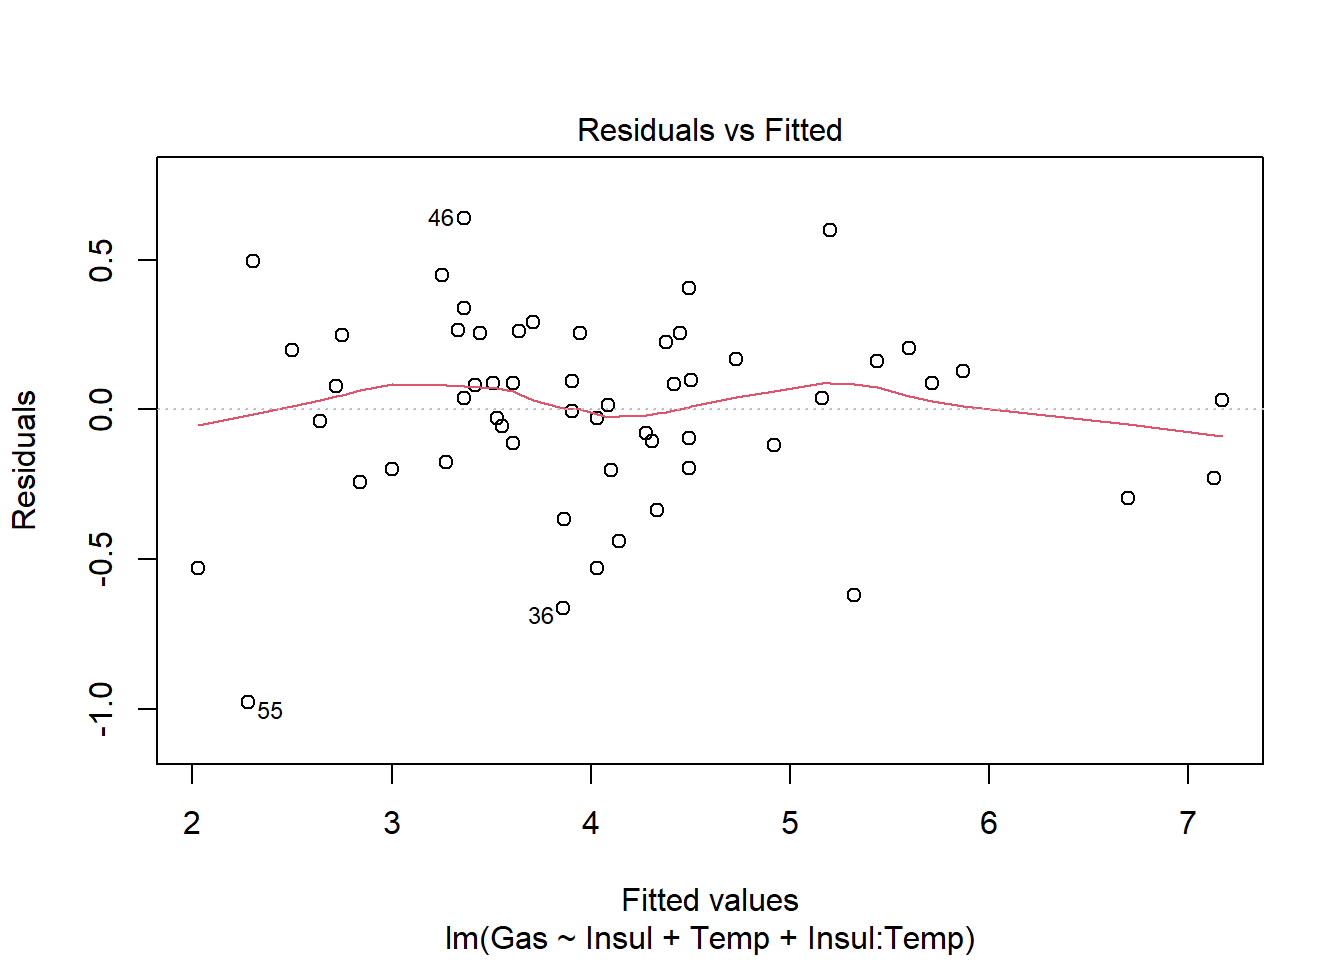
\includegraphics{_main_files/figure-latex/unnamed-chunk-332-1.pdf}

Once we fit a model and we're reasonably confident that it's a good model, we may want to visualize it. Three packages in R that help with this are \textbf{emmeans}, \textbf{effects}, and \textbf{ggeffects}. We briefly demonstrate the \textbf{ggeffects} package.

You need to first install the \textbf{ggeffects} package as it does not come with the base R installation. Once installed, load using the \texttt{library()} function.

Once loaded, we can get a basic visualization of our model by using the \texttt{plot()} and \texttt{ggpredict()} functions. This is particularly useful for models with interactions. Use the \texttt{terms} argument to specify which variables to plot. Below we list ``Temp'' first, which will plot ``Temp'' on the x axis. Then we list ``Insul'', the grouping variable, to indicate we want a separate fit for each level of ``Insul''.

\begin{Shaded}
\begin{Highlighting}[]
\SpecialCharTok{\textgreater{}} \CommentTok{\# install.pacakges("ggeffects")}
\ErrorTok{\textgreater{}} \FunctionTok{library}\NormalTok{(ggeffects)}
\SpecialCharTok{\textgreater{}} \FunctionTok{plot}\NormalTok{(}\FunctionTok{ggpredict}\NormalTok{(m, }\AttributeTok{terms =} \FunctionTok{c}\NormalTok{(}\StringTok{"Temp"}\NormalTok{, }\StringTok{"Insul"}\NormalTok{)))}
\end{Highlighting}
\end{Shaded}

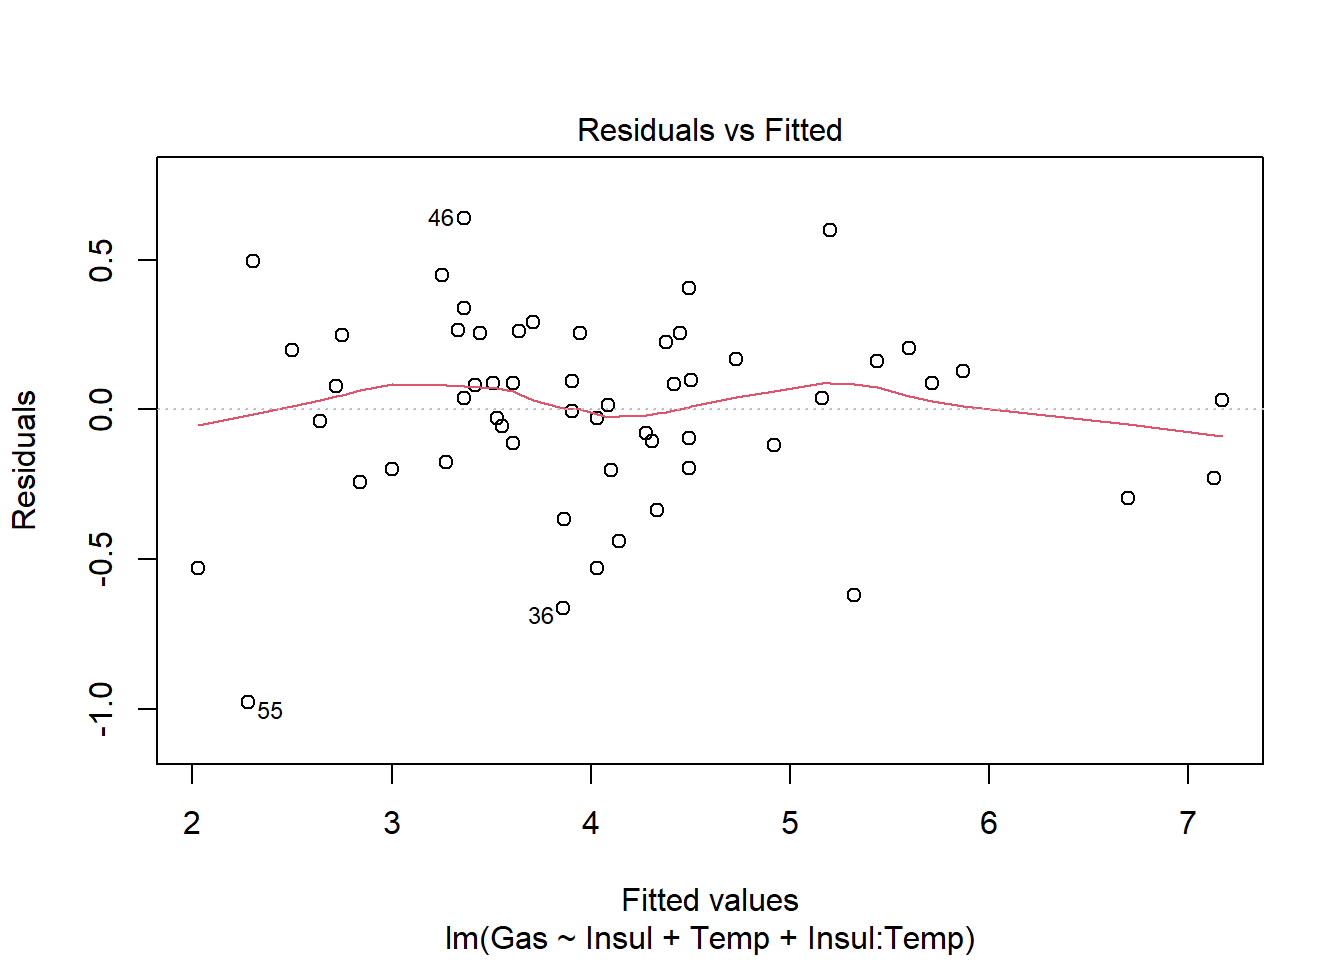
\includegraphics{_main_files/figure-latex/unnamed-chunk-333-1.pdf}

We see that after installing insulation, gas consumption fell considerably, and that the effect of temperature on gas consumption is less pronounced.

\hypertarget{logistic-regression}{%
\section{Logistic regression}\label{logistic-regression}}

Analyzing if or how the variability of a binary variable depends on one or more predictor variables.

\hypertarget{python-50}{%
\subsubsection*{Python}\label{python-50}}
\addcontentsline{toc}{subsubsection}{Python}

\hypertarget{r-50}{%
\subsubsection*{R}\label{r-50}}
\addcontentsline{toc}{subsubsection}{R}

  \bibliography{book.bib,packages.bib}

\end{document}
